%-----------------------------------------------------------------------
%
% File Name: thesis.tex
%
% Author: Nitz, A.
%
% Revision: $Id$
%
%-----------------------------------------------------------------------
%%%%%%%%%%%%%%%%%%%%%%%%%%%%%%%%%%%%%%%%%%%%%%%%%%%%%%%%%%%%%%%%%%%%%%%%%%%%%%%
%%%%%%%%%%%%%%%%%%%%%%%%%%%%%%%%%%%%%%%%%%%%%%%%%%%%%%%%%%%%%%%%%%%%%%%%%%%%%%%

% document class and packages
\documentclass[12pt,notitlepage]{report}
\usepackage{setspace}
\usepackage{graphicx}\usepackage{latexsym}
% \usepackage{iopams}

\usepackage{syrthesis}
% \usepackage{color}
\usepackage{amsmath,mathtools}
\usepackage{acronym}
\usepackage{amssymb}
\usepackage{adjustbox}
\usepackage{amsfonts}
\usepackage{rotating}
\usepackage{tensor}
\usepackage{lscape}
\usepackage{bm}
\usepackage{units} %  do things like \units[1.234]{sec}i
% \usepackage{chapterfolder} % Organize the graphics etc of each chapter in a sub-directory
\usepackage{amsopn, amstext, wasysym}
\usepackage{colonequals}
\usepackage{subfigure}
\usepackage{rotating}
\usepackage{braket}
\usepackage{multirow}
\usepackage{xspace}
\usepackage[usenames,dvipsnames]{color}

\usepackage[bookmarksnumbered, bookmarksopen, breaklinks, colorlinks, linkcolor=blue, citecolor=magenta]{hyperref}
\usepackage{bibunits}

\usepackage{url}
\usepackage{alltt}

\usepackage{ulem}
\normalem
\DeclareGraphicsExtensions{.eps,.pdf,.png}
\usepackage{epstopdf}
\usepackage[justification=centering]{caption}
%%%%%%%%%%%%%%%%%%%%%%%%%%%
%%% NINJA-2 packages
%%%%%%%%%%%%%%%%%%%%%%%%%%%%%
\usepackage{dcolumn}
\usepackage{units}
%%%%%%%%%%%%%%%%%%%%%%%%%%%
\makeatletter
\let\protect\relax
{\catcode`\|=\active
  \xdef\InnerProduct{\protect\expandafter\noexpand\csname InnerProduct
\endcsname}
  \expandafter\gdef\csname InnerProduct \endcsname#1{%
    \begingroup
    \ifx\SavedDoubleVert\relax
    \let\SavedDoubleVert\|\let\|\IpDoubleVert
    \fi
    \mathcode`\|32768\let|\IPVert
    \left({#1}\right)
    \endgroup
  }
}
\def\IPVert{\@ifnextchar|{\|\@gobble}% turn || into \|
     {\egroup\,\mid@vertical\,\bgroup}}
\def\IPDoubleVert{\egroup\,\mid@dblvertical\,\bgroup}
\let\SavedDoubleVert\relax
\def\midvert{\egroup\mid\bgroup}
\def\SetVert{\@ifnextchar|{\|\@gobble}% turn || into \|
    {\egroup\;\mid@vertical\;\bgroup}}
\def\SetDoubleVert{\egroup\;\mid@dblvertical\;\bgroup}
\def\mid@vertical{\mskip1mu\vrule\mskip1mu}
\def\mid@dblvertical{\mskip1mu\vrule\mskip2.5mu\vrule\mskip1mu}
\makeatother
\usepackage{braket}

\pdfoutput=1

\hbadness=10000

%%%%%%%%%%%%%%%%%%%%%%%%%%%%%%%%%%%%%%%%%%%%%%%%%%%%%%%%%%%%%%%%%%%%%%%%%%%%%%%
% journal definitions
%%%%%%%%%%%%%%%%%%%%%%%%%%%%%%%%%%%%%%%%%%%%%%%%%%%%%%%%%%%%%%%%%%%%%%%%%%%%%%%
\newcommand{\apj}{{\it Astrophysical J.}}
\newcommand{\apjl}{{\it Astrophysical J.}}
\newcommand{\aap}{{\it Astron. and Astrophys.}}
\newcommand{\cmp}{{\it Commun. Math. Phys.}}
\newcommand{\grg}{{\it Gen. Rel. Grav.}}
\newcommand{\cqg}{{\it Class. Quant. Grav.}}
\newcommand{\lr}{{\it Living Reviews in Relativity}}
\newcommand{\mnras}{{\it Mon. Not. Roy. Astr. Soc.}}
\newcommand{\pr}{{\it Phys. Rev.}}
\newcommand{\prl}{{\it Phys. Rev. Lett.}}
\newcommand{\pra}{{\it Phys. Rev. A}}
\newcommand{\prd}{{\it Phys. Rev. D}}
\newcommand{\nat}{{\it Nature}}
\newcommand{\prsl}{{\it Proc. R. Soc. Lond. A}}
\newcommand{\ptrsl}{{\it Phil. Trans. Roy. Soc. London}}
\newcommand{\rmp}{{\it Rev. Mod. Phys.}}

%%%%%%%%%%%%%%%%%%%%%%%%%%%%%%%%%%%%%%%%%%%%%%%%%%%%%%%%%%%%%%%%%%%%%%%%%%%%%%%
% new command definitions
%%%%%%%%%%%%%%%%%%%%%%%%%%%%%%%%%%%%%%%%%%%%%%%%%%%%%%%%%%%%%%%%%%%%%%%%%%%%%%%
\newcommand{\half}{\frac{1}{2}}
\newcommand{\ospsd}{\ensuremath{S_n\left(\left|f_{k}\right|\right)}}

\newcommand{\msun}{M_\odot}
\newcommand{\chisq}{\chi^2}
\newcommand{\newsnr}{\rho_{\textrm{new}}}
\newcommand{\erf}{\mathrm{erf}}

%%%%%%%%%%%%%%%%%%%%%%%%%%%%%%%%%%%%%%%%%%%%%%%%%%%%%%%%%%%%%%%%%%%%%%%%%%%%%%%
% more new commands
%%%%%%%%%%%%%%%%%%%%%%%%%%%%%%%%%%%%%%%%%%%%%%%%%%%%%%%%%%%%%%%%%%%%%%%%%%%%%%%
\newcommand{\Sum}{\displaystyle\sum\limits}
\newcommand{\Int}{\displaystyle\int\limits}
\newcommand{\ii}{{\rm i}}
\newcommand{\D}{\mathrm{d}}
\newcommand{\eff}{\mathrm{eff}}
\newcommand{\phys}{\mathrm{phys}}
\newcommand{\real}{\mathrm{real}}
\newcommand{\peak}{\mathrm{peak}}
% \newcommand{\EOB}{\mathrm{EOB}}
\newcommand{\NR}{\mathrm{NR}}
\newcommand{\RD}{\mathrm{RD}}
\newcommand{\Olap}{\mathcal{O}}
\newcommand{\FF}{\mathcal{FF}}
\newcommand{\MM}{\mathrm{MM}}
\newcommand{\EFF}{\mathrm{EFF}}
\newcommand{\X}{\mathrm{X}}
\newcommand{\Y}{\mathrm{Y}}
\newcommand{\Z}{\mathrm{Z}}
\newcommand{\horizon}{\mathrm{Horizon}}
\newcommand{\opt}{\mathrm{opt}}
\newcommand{\iso}{\mathrm{iso}}
\newcommand{\refr}{\mathrm{ref}}
\newcommand{\start}{\mathrm{start}}

\def\l({\left(}
\def\r){\right)}
\newcommand{\lt}{\left}
\newcommand{\rt}{\right}

%%%%%%%%%%%%%%%%%%%%%%%%%%%%%%%%%%%%%%%%%%%%%%%%%%%%%%%%%%%%%%%%%%%%%%%%%%%%%%%
% more new commands
%%%%%%%%%%%%%%%%%%%%%%%%%%%%%%%%%%%%%%%%%%%%%%%%%%%%%%%%%%%%%%%%%%%%%%%%%%%%%%%
\newcommand{\EOB}{\mathrm{EOBNRv2}}
\newcommand{\M}{\mathit{M}}
\newcommand{\bnk}{\mathrm{bank}}
\newcommand{\mn}{\mathrm{min}}
\newcommand{\mx}{\mathrm{max}}
\newcommand{\tr}{\mathrm{tr}}
\newcommand{\mm}{\mathrm{mm}}
\newcommand{\Hyb}{\mathrm{Hyb}}
\newcommand{\leftn}{\left|\left|}
\newcommand{\rightn}{\right|\right|}
\newcommand{\lefti}{\left\langle}
\newcommand{\righti}{\right\rangle}
\newcommand{\Mis}{\mathcal{M}}
\newcommand{\N}{\mathrm{N}}
\newcommand{\cyc}{\mathrm{cyc}}
\newcommand{\E}{\mathcal{E}}

\newcommand{\red}{\textcolor{red}}
\newcommand{\blue}{\textcolor{blue}}
\newcommand{\etal}{\textit{et~al}\@ifnextchar{\relax}{.\relax}{\ifx\@let@token.\else\ifx\@let@token~.\else.\@\xspace\fi\fi}}


%% Macros for comments
\newcommand\fake[1]{\textcolor{red}{#1}}
\newcommand\checkme[1]{\textcolor{blue}{\textbf{#1}}}
\newcommand{\Note}[1]{\textcolor{red}{\textbf{[#1]}}}
% \newcommand\checked[1]{#1}
\newcommand\marginnote[2]{%
  \mbox{}\marginpar{\raggedleft\hspace{0pt}\scriptsize
    \textcolor{blue}{#1: #2}}}


\newcommand\weakheader[1]{
\vspace*{5mm}
\noindent {\it #1}
\vspace*{5mm}
}

\usepackage{hyperref} 

\begin{document}
\Abstract{%%%%%%%%%%%%%%%%%%%%%%%%%%%%%%%%%%%%%%%%%%%%%%
%%%%%%% ABSTRACT
%%%%%%%%%%%%%%%%%%%%%%%%%%%%%%%%%%%%%%%%%%%%%%

In this dissertation we study gravitational-wave searches for 
binary neutron star and neutron star - black hole coalescences. 
We determine the accuracy of post-Newtonian approximations as gravitational-wave
templates in matched-filter based searches for NSBH mergers.
We test a geometric method to generate template banks for BNS and NSBH mergers where
the components have intrinsic spin, and estimate the sensitivity to
astrophysical sources of searches that use these banks during Advanced LIGO.
We explore simplifications and optimizations to the search pipeline used 
during S6/VSR2,3 gravitational-wave searches. We investigate methods for regenerating
template banks as the noise behavior of a detector changes over time. We further
investigate changes to the algorithim for determining coincidence between
candidates from multiple-detectors.
Finally, we develop a focused search for binary neutron stars, and test improvements
to its configuration using LIGO detector data from the most recent science
run.
}

\title{
The effects of spinning neutron stars and black holes on the seach for gravitational-waves from binary neutron star and neutron star -- black hole mergers.
}
\author{Alexander Harvey Nitz}
\pastdegrees{}
\majorprof{Duncan A. Brown}
\submitdate{August 2015}
\degree{Doctor of Philosophy}
\program{Physics}
\copyrightyear{2015}

\majordept{Physics}
\havededicationtrue
\dedication{to\\ ....}
\haveminorfalse
\copyrighttrue
\doctoratetrue

%\figurespagefalse
%\tablespagefalse
%\signedtitlepfalse

% \doublespacing
 \Abstract{
 %%%%%%%%%%%%%%%%%%%%%%%%%%%%%%%%%%%%%%%%%%%%%%
%%%%%%% ABSTRACT
%%%%%%%%%%%%%%%%%%%%%%%%%%%%%%%%%%%%%%%%%%%%%%

In this dissertation we study gravitational-wave searches for 
binary neutron star and neutron star - black hole coalescences. 
We determine the accuracy of post-Newtonian approximations as gravitational-wave
templates in matched-filter based searches for NSBH mergers.
We test a geometric method to generate template banks for BNS and NSBH mergers where
the components have intrinsic spin, and estimate the sensitivity to
astrophysical sources of searches that use these banks during Advanced LIGO.
We explore simplifications and optimizations to the search pipeline used 
during S6/VSR2,3 gravitational-wave searches. We investigate methods for regenerating
template banks as the noise behavior of a detector changes over time. We further
investigate changes to the algorithim for determining coincidence between
candidates from multiple-detectors.
Finally, we develop a focused search for binary neutron stars, and test improvements
to its configuration using LIGO detector data from the most recent science
run.

 }
 
\beforepreface
\prefacesection{Preface}
%%%%%%%%%%%%%%%%%%%%%%%%%%%%%%%%%%%%%%%%%%%%%%%%5
%%%%%%%%%% PREFACE
%%%%%%%%%%%%%%%%%%%%%%%%%%%%%%%%%%%%%%%%%%%%%%%%

The work presented in this thesis stems from my participation in the
LIGO Scientific Collaboration (LSC) and the NINJA-2 Collaboration.  This
work does not reflect the scientific opinion of the LSC and it was not
reviewed by the collaboration.

\vspace*{0.5cm}

\noindent Chapter~\ref{ch:EOBF2_Effectualness} is based on material from

\vspace*{0.25cm}

\noindent D. A. Brown, P. Kumar and A. H. Nitz, ``Template banks to 
search for low-mass binary black holes with Advanced Gravitational-wave 
detectors,''
{\it Phys. Rev. D} {\bf 87}, 082004 (2013)

\vspace*{0.5cm}

\noindent Chapter~\ref{ch:NRHyb_bank} is based on material from

\vspace*{0.25cm}

\noindent P. Kumar, I. MacDonald, D. A. Brown, H. P. Pfeiffer, K. Cannon,
M. Boyle, L. E. Kidder, A. H. Mroue, B. Szilagyi and A. Zeninoglu, 
``Template banks for binary black hole searches with numerical relativity
waveforms,''
{\it Phys. Rev. D} {\bf 89}, 042002 (2014)

\vspace*{0.5cm}

\noindent Chapter~\ref{ch:ninja2} is based on material from

\vspace*{0.25cm}

\noindent The LIGO Scientific Collaboration, the Virgo Collaboration, 
the NINJA-2 Collaboration, ``The NINJA-2 project: 
Detecting and characterizing gravitational waveforms modelled using 
numerical binary black hole simulations,''
{\it arXiv:1401.0939} (2014) {\rm Submitted to Classical and Quantum Gravity}

\vspace*{0.5cm}

\noindent Chapter~\ref{ch:insSFIMRI} is based on material from

\vspace*{0.25cm}

\noindent E. A. Huerta, P. Kumar, D. A. Brown, 
``Accurate modeling of intermediate-mass-ratio inspirals:
Exploring the form of the self-force in the intermediate-mass-ratio regime,''
{\it Phys. Rev. D} {\bf 86}, 024024 (2012)

\vspace*{0.5cm}

\noindent Chapter~\ref{ch:imrSFIMRI} is based on material from

\vspace*{0.25cm}

\noindent E. A. Huerta, P. Kumar, J. R. Gair, S. T. McWilliams, 
``Self-forced evolutions of an implicit rotating source:
a natural framework to model comparable and intermediate mass-ratio 
systems from inspiral through ringdown,''
{\it arXiv:1403.0561} (2014) {\rm Submitted to Phys. Rev. D}

\vspace*{0.5cm}


\prefacesection{Acknowledgments}
%%%%%%%%%%%%%%%%% Acknowledgements
I've had the privilege over the past several years to work with numerous physicists,
make friends, and build connections through my membership in the LIGO Scientific
collaboration. To those that I fail to thank here, please know that I am appreciative,
and that I intend no slight. 

\noindent I would first like to express my deepest gratitude and thanks to my advisor,
Duncan Brown. His broad knowledge of gravitational-wave astronomy and his
exuberance have been an inspiration. I am indebted to him for his
guidance, encourgement, and especially his patience.

\noindent I would also like to thank the members of my defense committee --- Robert Moucha,
Martin Forstner, Liviu Movilenau, Simon Catterall, and Mitchell Soderberg --- 
for taking time out of theri busy schedule to read and critique my work.

\noindent I would also like to thank Keith Riles for introducing me to LIGO,
without whom, I would not have had the amazing experiences and challenges that
come with working on the frontiers of gravitational-wave phsyics. 
%%%


%\prefacesection{Conventions}
%%%%%%%%%%%%%%%%%%%%%%%%%%%%%%%%
%%%%%%% CONVENTIONS
%%%%%%%%%%%%%%%%%%%%%%%%%%%%%%%

We adopt the Einstein summation convention where repeated indices are
summed over.  
%
The signature of spacetime is taken to be $(-1,+1,+1,+1)$.

\noindent Except where otherwise noted we work in geometric units where
$G=c=1$.  We will often measure masses in multiples of the mass of the
sun $1 \msun \approx 1.99 \times 10^{30}$ kg 

\vspace{0.5cm}

\noindent We define the Fourier transform of a function of time $g(t)$ to be
$\tilde{g}(f)$, where
%
\begin{equation*}
\tilde{g}(f)=\int_{-\infty}^\infty g(t)\, e^{- 2 \pi i f t}\, dt
\end{equation*}
%
and the inverse Fourier transform is
%
\begin{equation*}
g(t)=\int_{-\infty}^\infty \tilde{g}(f)\, e^{2 \pi i f t}\, dt
\end{equation*}
%
This convention differs from that used in some gravitational-wave
literature, but is the adopted convention in the LIGO Scientific
Collaboration.

% \vspace{0.5cm}
% 
% \noindent The time-stamps of interferometer data are measured in
% Global Positioning System (GPS) seconds: seconds since 00:00.00 UTC
% January 6, 1980 as measured by an atomic clock.


\afterpreface

\Chapter{Introduction}
\label{ch:introduction}
In 1915, Albert Einstein published his theory of general relativity, a 
geometric theory of gravitation that sought to expand upon Newtonian 
mechanics and provide a complete description of gravity and its 
relationship with space and time. Einstein theorized that space 
and time were deeply related and existed together as a manifold 
called spacetime. Matter with energy and momentum 
existing in this manifold would create 
curvature in spacetime. Gravitational forces were the result of 
matter following geodesic curves in spacetime. This concept can 
be summarized in the Einstein field equation, which is presented 
as,
\begin{equation}
G_{\mu\nu} = 8\pi T_{\mu\nu}
\label{eq:EFE}
\end{equation}
where $G_{\mu\nu}$ is the Einstein tensor, which describes the 
curvature of spacetime, $T_{\mu\nu}$ is the 
stres-energy tensor, which describes the energy and momentum in 
spacetime, and  $G=c=1$. The Einstein tensor is defined as,
\begin{equation}
G_{\mu\nu} = R_{\mu\nu} - \frac{1}{2}Rg_{\mu\nu}
\end{equation}
where $R_{\mu\nu}$ is the Ricci curvature tensor and $g_{\mu\nu}$ is 
the metric tensor for the manifold.

An interesting result that arises from this formalism is the 
existence of gravitational waves, which are perturbations in 
spacetime caused by certain types of time-varying mass distributions. 
To describe gravitational waves, we consider 
a Minkowski metric with a small perturbation. The Minkowski metric 
is a flat spacetime metric defined as
\begin{equation}
\eta_{\mu\nu} = 
  \begin{pmatrix}
   -1 & 0 & 0 & 0 \\
    0 & 1 & 0 & 0 \\
    0 & 0 & 1 & 0 \\
    0 & 0 & 0 & 1
  \end{pmatrix}
\end{equation}
where $\mu = 0$ corresponds to the time coordinate and $\mu = {1,2,3}$ 
correspond to the spatial coordinates. In examples, we will use the coordinate 
convention $(x^0,x^1,x^2,x^3) = (ct,x,y,z)$. 
The full spacetime metric, $g_{\mu\nu}$, is then constructed as a 
linear perturbation on the Minkowski metric,
\begin{equation}
g_{\mu\nu} = \eta_{\mu\nu} + h_{\mu\nu}
\end{equation}
where $h_{\mu\nu}$ is the metric perturbation and $|h_{\mu\nu}| \ll 1$.
From here, we follow the convention of Saulson \cite{Saulson:1994} to arrive at the general 
form of a gravitational wave.
At this point it is very useful to move into the transverse traceless 
gauge where coordinates on the manifold are defined by the geodesic 
motion of freely-falling test masses. In this gauge, the weak field 
vacuum solution of the Einstein field equation becomes a wave equation: 
\begin{equation}
\square h_{\mu\nu} = 0.
\end{equation}
The solutions to this differential equation will be plane waves of 
the form
\begin{equation}
h_{\mu\nu} = C_{\mu\nu}e^{i(2\pi ft - \vec{k}\cdot\vec{x})}
\end{equation}
where $C_{\mu\nu}$ is the wave amplitude, $f$ is the frequency, 
and $\vec{k}$ is the wave vector which indicates the direction of 
propagation \cite{Carroll}.

For example, consider the case of a gravitational 
wave propogating along the $\hat{z}$-axis.
When the conditions of the transverse traceless gauge are applied, 
the resulting form of $h_{\mu\nu}$ is 
\begin{equation}
h_{\mu\nu} = 
  \begin{pmatrix}
    0 & 0 & 0 & 0 \\
    0 & h_+ & h_x & 0 \\
    0 & h_x & -h_+ & 0 \\
    0 & 0 & 0 & 0
  \end{pmatrix}
\end{equation}
where the diagonal and off-diagonal terms represent two polarizations 
of the resulting gravitational wave, called "h-plus" and "h-cross" 
respectively.
We can see the effects of this perturbation by observing the  
spacetime interval on the manifold. The spacetime interval is defined as 
\begin{equation}
ds^2 = dx^\mu g_{\mu\nu}dx^\nu.
\end{equation}
Substituting in our perturbed metric for $g_{\mu\nu}$, we find that 
the spacetime interval can be broken up into a standard Minkowski line 
element and a perturbation due to $h_{\mu\nu}$.
\begin{equation}
ds^2 = dx^\mu (\eta_{\mu\nu} + h_{\mu\nu})dx^\nu \\
\end{equation}
\begin{equation}
ds^2 = dx^\mu \eta_{\mu\nu} dx^\nu + dx^\mu h_{\mu\nu}dx^\nu
\label{eq:spacetime}
\end{equation}

As an example, we present the case of a plus-polarized gravitational wave 
propagating in the $\hat{z}$ direction and observe the effect of the perturbation 
on the spacetime interval. The perturbation will have the form 
\begin{equation}
h_{\mu\nu} = 
  \begin{pmatrix}
    0 & 0 & 0 & 0 \\
    0 & h_+ & 0 & 0 \\
    0 & 0 & -h_+ & 0 \\
    0 & 0 & 0 & 0
  \end{pmatrix}
\end{equation}
Using the coordinate convention of $(ct,x,y,z)$, the unperturbed
spacetime interval is given as: 
\begin{equation}
ds^2 = -c^2 dt^2 + dx^2 + dy^2 + dz^2.
\end{equation}
Since the perturbation is spatially transverse to the direction of 
propagation, the ct- and z-coordinates will not be modulated by the 
gravitational wave. The x- and y-coordinates will be modulated  
according to equation \ref{eq:spacetime}. The resulting spacetime 
interval is
\begin{equation}
ds^2 = -c^2 dt^2 + (1 + h_+)dx^2 + (1 - h_+)dy^2 + dz^2.
\end{equation}
This shows that a gravitational wave propogating along the $\hat{z}$-axis 
will differentially stretch and squeeze spacetime in the transverse 
axes. The exact form of $h_+$ will depend on the source of the 
gravitational waves. A visualization of this stretching and squeezing 
is shown in Figure \ref{fig:polarizations}\cite{Polarization}. The cross polarization  
stretches and squeezes at a 45 degree angle relative to the plus 
polarization.

\begin{figure}[ht!]
\includegraphics[width=\textwidth]{figures/introduction/polarisations2}
\caption[Plus and cross polarizations]{Plus and cross polarizations %
         of a gravitational wave.}
\label{fig:polarizations}
\end{figure}

The Advanced LIGO interferometers are designed to be sensitive 
to this differential stretching and squeezing by constructing orthogonal 
optical cavities. A gravitational wave passing through an aLIGO interferometer 
will differentially 
modulate the lengths of the optical cavities, creating an interference 
pattern at the output of the instrument that can be searched for 
gravitational wave signals. The layout and gravitational wave readout scheme 
of the interferometers is discussed below.

\section{The Advanced LIGO Interferometers}\label{sec:aligo}

The Advanced LIGO (aLIGO) interferometers are a pair of dual-recycled Michelson interferometers 
that employ 4km long Fabry-Perot cavities in their arms to increase the interaction time with a 
gravitational wave signal. 
Figure \ref{fig:aligo} shows a simplified layout of an aLIGO interferometer. 

\begin{figure}[ht!]
\includegraphics[width=\textwidth]{figures/introduction/ALIGO_layout}
\caption[Layout of Advanced LIGO]{Layout of Advanced LIGO}
\label{fig:aligo}
\end{figure}

At the input to an aLIGO interferometer is a solid-state Nd:YAG laser that provides laser light 
at a wavelength of 1064 nm. Not included in Figure \ref{fig:aligo} are frequency and 
intensity stabilization control loops designed to provide as stable a laser source as 
possible for the experiment. This stabilized laser is called the pre-stabilized laser 
(PSL). The laser light is passed through a series of 
electro-optic modulators (EOM) where radio-frequency (RF) sidebands are generated 
and imparted onto the light. These RF sidebands are used to control auxiliary optical 
degrees of freedom in the interferometer. The beam is then passed through the 
input mode cleaner (IMC), which rejects higher order spatial modes of the beam 
and transmits a circular TEM00 mode to be used in the instrument.

Once the beam has been stabilized in frequency and intensity and the higher order 
optical modes have been stripped away, it is transmitted through the power 
recycling mirror and enters the vertex of the interferometer. In the vertex, 
the beam is split 50/50 by the beamsplitter. Half of the light is directed toward  
the input test mass (ITM) of the X-arm and half of the light is directed  
toward the ITM of the Y-arm. As mentioned previously, the aLIGO arms are not 
single bounce cavities; they are comprised of Fabry-Perot cavities that allow the 
light to circulate in the arm cavities multiple times. The light is stored in 
the arm cavities for $\sim$1ms, trapped between the highly reflective surfaces 
of the ITM and the end test mass (ETM), before it is transmitted back through 
the ITM and into the vertex.

When a gravitational wave passes through an aLIGO inteferometer, the distance
between the ITM and ETM of each arm is modulated, causing the light to have a
longer or shorter travel time as it traverses the arm. Since gravitational
waves expand space in one direction while the orthogonal direction contracts,     
the X- and Y-arms will experience differential changes in length. When light
from the arms is recombined at the beamsplitter, there will be a difference
in phase between the two beams as they have traveled different paths. The 
resulting light from this recombination of phase shifted beams is called the 
antisymmetric part of the output. The part of the beam that is recombined 
in phase is called the symmetric part of the output.

The beams returning from each arm are recombined at the beamsplitter. The 
symmetric part of the beam 
will be sent back toward the power recycling mirror. The power recycling mirror 
forms a resonant cavity with the ITMs, allowing for light at the symmetric 
port of the beamsplitter to be added coherently to incoming light from the PSL and 
increasing the effective power in the vertex. This increase in effective power 
is known as the power recycling gain. 

The antisymmetric part of the beam is sent toward the signal recycling mirror. 
The signal recycling cavity is used to tune the frequency response of the 
interferometer by adjusting the effective finesse of the coupled cavity 
formed by the signal recycling cavity and the arm cavities. 
If the light returning from the arms has accumulated some differential amount of 
phase as it traveled 
along the arms, perhaps from a gravitational wave modulating the length of each 
arm differentially, it will be transmitted through the signal recycling cavity 
and into the output mode cleaner (OMC). The OMC behaves similarly to the IMC, 
stripping away higher order optical modes and isolating the TEM00 mode of the 
beam. The transmitted, mode cleaned signal is then read out using a homodyne 
detection scheme on a DC photodiode. 

\subsection{DC Readout}

When a gravitational wave modulates the length of an arm cavity, the light 
traveling in that arm experiences a phase modulation. This phase modulation 
can be visualized by picturing the beam in frequency space. In figure 
\ref{fig:omc-freq}, the carrier beam frequency is designated as $f_0$. 
The phase modulation due to 
a gravitational wave signal introduces a frequency sideband at the 
gravitational wave frequency, which is in the 30-2000 Hz range. 
The 
RF sidebands used for auxiliary optical cavity control are offset from the 
carrier frequency by 9, 24, and 45 MHz. 
The RF sidebands, which in a 
homodyne detection scheme would only contribute shot noise to the output signal, 
are rejected by the OMC. The gravitational wave sidebands, however, are at a 
low enough frequency offset that they are within the cavity pole of the OMC 
and are allowed to transmit through the cavity.

Since the OMC DC photodiode measures power, it measures the square of the 
incident optical field and witnesses beat frequencies between different 
components of the light. If the RF sidebands have been filtered out by 
the OMC, the only remaining beat note will be that of the carrier beam ($f_0$) 
beating against the gravitational wave sideband ($f_0 + f_{GW}$). This beat note will 
appear as the difference in frequency between the two optical fields, 
leaving behind a signal in the 30-2000 Hz range ($f_{GW}$) and providing a 
natural demodulation inherent to the measurement process. 
The process of recovering the gravitational wave sideband using the 
carrier field as a reference is known as homodyne detection. 

\begin{figure}[ht!]
\includegraphics[width=\textwidth]{figures/introduction/omc-freq}
\caption[Sidebands and OMC cavity pole]{Frequency domain visualization of beam %
         at OMC. Grey dotted lines indicate the cavity pole. The gravitational %
         wave sidebands are within the cavity pole and are transmitted through %
         the OMC. The RF sidebands are in the MHz range and are rejected by the %
         OMC.}
\end{figure}\label{fig:omc-freq}

\section{Sources of Gravitational Waves}
Include that box with modeled, unmodeled, transient, and continuous.

CBCs are the bread and butter, expect BNS, NSBH, and BBH sources
Continuous waves from pulsars
Bursts from supernovae
Stochastic background


\section{Searching for Compact Binary Coalescences}

Steal this from O1 CBC DQ paper


\section{The Advanced Detector Network}

The Advanced Laser Interferometer Gravitational-Wave Observatory (aLIGO) is 
part of a worldwide effort to detect gravitational waves from astrophysical 
sources. The two aLIGO interferometers, one in Hanford, WA and one in 
Livingston, LA, are part of a growing network of ground-based interferometric 
gravitational wave detectors. Each aLIGO interferometer has 4km long arms 
arranged in an L-shaped configuration. A gravitational wave passing through 
an aLIGO interferometer will cause the arms to expand and contract, 
creating an interferometric signal at the output of the instrument. 
Section \ref{sec:aligo} contains a more detailed description of the aLIGO 
interferometers. 

There are a number of other interferometric gravitational wave detectors 
being built and commissioned for future use in collaboration with aLIGO.
The Advanced VIRGO detector is being built and commissioned in Cascina, Italy. 
When it is fully commissioned, VIRGO will be joining LIGO in observing runs. 
The VIRGO interferometer has 3km arms, which should provide enough 
sensitivity to allow for triangulation of astrophysical sources.

The GEO600 detector, located in Hanover, Germany is an interferometer built in 
collaboration between Germany and the United Kingdom. 
GEO600 is an extremely valuable test bed for interferometric technologies,
including quantum optics and homodyne detection. However, with 600m arms, GEO600 
is unlikely to be sensitive enough to witness expected astrophysical sources.

The KAGRA detector, located underground in the Kamioka mine in Japan, 
is in its commissioning phase. KAGRA has 3 km long arms and, 
unlike other gravitational wave interferometers, employs cryogenics to 
reduce thermal noise in its optics. When complete, KAGRA should be 
sensitive enough to contribute to the worldwide detector network.

Include that cool picture of the advanced detector network.


\Chapter{Pipelines to Search for Gravitational-waves from Compact Binary Coalescences}
\label{ch:search}
\section{Introduction}

Searches for gravitational waves from compact object
binaries containing neutron stars and stellar-mass black holes have been
performed using the first-generation LIGO and Virgo detectors in LIGO's six
science runs (S1--S6) and three Virgo science runs
(VSR1--VSR3)~\cite{Abbott:2003pj,Abbott:2005pe,Abbott:2005kq,Abbott:2007xi,Abbott:2007ai,Abbott:2009tt,Abbott:2009qj,Abadie:2010yba,Abadie:2011nz}.
Construction of the Advanced LIGO (aLIGO) detectors~\cite{TheLIGOScientific:2014jea} is now complete and the
first aLIGO observing runs are scheduled for autumn 2015~\cite{Aasi:2013wya}.
The Advanced Virgo (AdV) detector~\cite{Acernese:2015gua} is scheduled to join this network in 2016.
When these second-generation detectors reach design sensitivity, it is
predicted that they will observe on the order of $10$ coalescence events per
year~\cite{Abadie:2010cf}. Binaries containing neutron stars and stellar-mass
black holes are likely to be the first sources observed by aLIGO and AdV. 

Gravitational waves from compact binary coalescence have three distinct
phases: an \emph{inspiral} consisting of a wave of slowly increasing amplitude
and frequency, a \emph{merger} which can be calculated using numerical
simulations, and a \emph{post-merger} signal as the binary stabilizes into a final
state. If the total mass of the binary is lower than $M \lesssim 12\,
M_\odot$~\cite{Buonanno:2009zt,Brown:2012nn}
and the angular momenta of the compact objects (their \emph{spin}) is
small~\cite{Nitz:2013mxa,Kumar:2015tha}
(as is the case for binary neutron stars), then the inspiral phase can be 
well modeled using the post-Newtonian approximations (see e.g.
Ref.~\cite{Blanchet:2013haa} for a review).  For higher mass and higher-spin
binaries, analytic models tuned to numerical relativity can provide accurate
predictions for the gravitational waves from compact 
binaries~\cite{Buonanno:1998gg,Pan:2009wj,Damour:2012ky,Taracchini:2013rva,Damour:2014sva}. 

Ground-based gravitational-wave detectors produce a calibrated strain signal
$s(t)$, which is sensitive to gravitational waves incident on the detector's
arms~\cite{Abadie:2010px}. In addition to possible signals, the strain data contain two classes of
noise: (i) a primarily stationary, Gaussian noise component from fundamental
processes such as thermal noise, quantum noise, and seismic noise coupling
into the detector; and (ii) non-Gaussian noise transients of instrumental and
environmental origin. Since the gravitational-wave signal from compact
binaries is well-modeled and the expected amplitude of astrophysical signals is
comparable to the amplitude of the noise,
matched filtering is used to search for signals in the detector data~\cite{Allen:2005fk}.  Since
we do not \emph{a priori} know the parameters of the compact
binaries we may detect, a \emph{bank} of template waveforms is constructed that spans the astrophysical
signal space~\cite{Sathyaprakash:1991mt,Dhurandhar:1992mw,Owen:1995tm,Owen:1998dk,Babak:2006ty,Cokelaer:2007kx,Brown:2012qf,Keppel:2013yia,Keppel:2013uma}. These banks are designed so that the loss in event rate caused by
their discrete nature is typically no more than 10\%. The exact placement of the
templates depends on the noise power spectral density of the detector data. To
mitigate the effect of the non-Gaussian noise transients in the search, we
require that any signal be seen with consistent parameters (compact objects'
spins and masses and the signal's time of arrival) in the detector network. Additional
statistical tests are applied to mitigate the effect of non-Gaussian
noise transients~\cite{Allen:2004gu}; these are often called \emph{signal-based vetoes}. The 
matched-filter signal-to-noise ratio and the additional statistical tests are used to
create a numerical detection statistic for candidate signals. To assign a
statistical significance to these detection candidates, the network's false-alarm rate is computed as a function of the detection statistic for the
noise background.

Executing the steps described above is the task of the \emph{search pipeline.}
While the basic steps remain the same, different choices can be made to
create various configurations and topologies for a search pipeline. The search
pipelines used in the last joint LIGO-Virgo science run (S6/VSR2,3) used the
\texttt{ihope} search pipeline to search for compact
binaries~\cite{Babak:2012zx}. The \texttt{ihope} pipeline, as well as the
pipelines used in previous LIGO-Virgo
searches~\cite{Brown:2004pv,Brown:2005zs}, are \emph{offline} search
pipelines. These pipelines analyze the data in a batch mode, processing
of the order of one week of data from the network. Offline batch
processing allows the pipeline to incorporate additional information about the
quality of the detector data or search tuning that is not available in real
time~\cite{Aasi:2012wd,Aasi:2014mqd}, and to produces a systematic false-alarm rate
estimation of candidates by using large samples of the noise background before
and after the time of a signal. Batch processing also allows the pipeline to
take advantage of the computationally efficient Fast Fourier Transform (FFT)
when implementing matched filtering~\cite{Allen:2005fk}, and allows
computational tasks to be parallelized over time and binary parameters for
efficient implementation on large computing clusters~\cite{Brown:workflow}.

\section{Assessing Waveform and Template Bank Effectiveness}
\label{sec:analytic_vol}

In the absense of non-Gaussian noise, we can create analytic measures of the
faithfulness and effectiveness of the waveform models and template banks that 
will be used to search for gravitational waves. In this section we describe 
the methods and the terminology that we will use in the rest of this work.

The ``overlap'' between two waveforms $h_1$ and $h_2$ is defined as
%
\begin{equation}
 \mathcal{O}(h_1,h_2) = (\hat{h}_1|\hat{h}_2) =
\dfrac{(h_1|h_2)}{\sqrt{(h_1|h_1)(h_2|h_2)}},
\end{equation}
%
where $(h_1,h_2)$ denotes the noise-weighted inner product
%
\begin{equation}
(h_1|h_2) = 4 \, \mathrm{Re}
\int^{\infty}_{f_{\mathrm{min}}}\dfrac{\tilde{h}_1(f)\tilde{h}_2^*(f)}{S_n(f)} 
df.
\end{equation}
%
Here, $S_n(f)$ denotes the one sided \ac{PSD} of the noise in the
interferometer.

As gravitational wave searches for binary mergers analytically maximize over an
overall phase and time shift, we define the ``match'' between two waveforms
to be the overlap maximized over a phase and time shift
%
\begin{equation}
\mathcal{M}(h_1,h_2) =
\underset{\phi_c,t_c}{\max}(\hat{h}_1|\hat{h}_2(\phi_c,t_c)).
\end{equation}
%
One can understand this match as the fraction of the optimal \ac{SNR} that would
be recovered if a template $h_1$ was used to search for a signal $h_2$.

We define the ``fitting-factor'' between a waveform $h_s$ with unknown
parameters
and a bank of templates $h_b$ to be the maximum match between $h_s$ and all the
waveforms in the template bank~\cite{Apostolatos:1995pj},
%
\begin{equation}
\mathrm{FF}(h_s) = \max_{h \in \{h_b\}} \mathcal{M}(h_s,h).
\end{equation}
%
The ``mismatch''
%
\begin{equation}
\mathrm{MM} = 1 - \mathrm{FF}(h_s)
\end{equation}
%
describes the fraction of \ac{SNR} that is lost due to the fact that the
template in the bank that best matches $h_s$ will not match it exactly due to
the discreteness of the bank and due to any disagreement between the waveform 
families used to model the templates and the signals. 

\section{Coincident Matched-Filter Search for Compact Binaries}
\label{s:search}

To search for coalescing compact binaries with LIGO and Virgo, the offline search
pipeline implements a coincident matched-filter search.  If the detector noise
was stationary and Gaussian, matched filtering alone would be sufficient to
determine the statistical significance of a signal. For such stationary noise, 
demanding that the signal is present in two or more detectors in the network 
(coincidence) would provide a sufficiently low false-alarm rate to claim a 
detection at a matched-filter network signal-to-noise ratio of 8; the signal 
strength used to estimate aLIGO's event rate in Ref.~\cite{Abadie:2010cf}.
However, the presence of non-stationary and non-Gaussian noise
transients (\emph{glitches})
in the detector noise increases the false-alarm rate at a given
signal-to-noise ratio and additional statistical tests must be used to separate
signals from noise. The output of the matched filter is combined with these
additional tests to create a new detection statistic for coincident detection
candidates. To determine the significance of these candidates, the noise
background must be estimated to create a map between the numeric value of the
detection statistic and the false-alarm rate (or, equivalently, false-alarm
probability). Background noise is estimated by performing coincidence tests on
detector data which has been time-shifted such that coincident candidates no
longer represents a coincident detection. The search pipeline consists of
several stages which are applied to the data to construct coincident detection
candidates and measure their significance. 

To search for gravitational waves from compact binaries, the search pipeline
first locates the data from the detectors, which is stored on disk. Analysis
of the week of data can be parallelized over time and over detector allowing
the search to execute multiple search programs simultaneously that process
small blocks of data for each detector. In the S6/VSR2,3 search, the 
analysis block size is set to $2048$ seconds.
The data is first used to construct the
template bank that will be used to matched filter the
data~\cite{Sathyaprakash:1991mt,Dhurandhar:1992mw,Owen:1995tm,Owen:1998dk,Babak:2006ty}.
The bank is constructed by specifying the boundaries of the target
astrophysical space and the desired \emph{minimal match}, the fractional loss in
matched-filter signal-to-noise ratio caused by the discrete nature of the bank.
The minimal match is chosen so that the bank is dense enough that any
gravitational wave in the target space can be recovered with a loss of
signal-to-noise ratio no greater than a chosen maximum, usually set to 3\%~\cite{Abbott:2011ys}. 
A metric is constructed on the signal space that
locally measures the fractional loss in signal-to-noise ratio for varying mass
parameters of the templates~\cite{Owen:1998dk}.  This metric (and hence
the template placement) depends on the power spectral density of the
detector noise. Since inspiral signals have more cycles at lower frequencies,
a detector with better low-frequency sensitivity relative to high frequencies
will have more discriminating power and thus require a denser bank to maintain
the desired minimal match.

The pipeline then matched filters the template waveforms against the data.
The matched filter consists of a weighted inner product in the frequency
domain used to construct the (squared) signal-to-noise ratio, given by
%
\begin{equation}
\rho^2(t) = \frac{(s|h_c)^2 + (s|h_s)^2}{(h_c|h_c)} \, ,
\label{eq:snr}
\end{equation}
%
where $h_c$ and $h_s$ are the two orthogonal phases of the 
%
\begin{equation}
(s|h)(t) = 4\int_{f_{low}}^{f_{high}} \frac{\tilde{s}(f)\tilde{h}^*(f)}{S_n (f)}e^{2\pi i f t}\, \mathrm{d}f.
\label{eq:ip}
\end{equation}
%
Here $\tilde{s}$ denotes the Fourier-transformed detector data and $\tilde{h}$
denotes the Fourier-transformed template waveform. As in the S6/VSR2,3 search,
each 2048 second block of data is sub-divided into fifteen $256$ second
segments, each overlapped by $128$ seconds. The noise power spectral
density $S_n(f)$ is computed by taking the bin-by-bin median of each of the power
spectral density of each of the fifteen segments. The fifteen segments are then each
matched filtered, with the first and last $64$ seconds of each segment
ignored, due to corruption of the filter by FFT
wrap-around~\cite{Allen:2005fk}

Times when the signal-to-noise ratio exceeds a pre-defined threshold are
considered gravitational-wave candidates, called
\emph{triggers}\cite{Allen:2005fk}. This threshold is set to a
signal-to-noise ratio of 5.5.  Since the signal-to-noise ratio can exceed
this threshold for many sample points around the time of a signal, clustering
is performed on these triggers in time, so that one trigger can be associated
with a signal. Template-length based clustering of 
Ref.~\cite{Allen:2005fk} was used in the S6/VSR2,3 search. 
For a sufficiently loud event, several nearby templates in the
bank may also produce triggers associated with the same signal and so
clustering over the template bank can also be used to limit the number of
triggers produced by the search. The S6/VSR2,3 search used a 30~ms time window
to cluster over the bank.

Since non-Gaussian noise transients in the data can also produce excursions in
the signal-to-noise ratio, an additional signal-based veto is then constructed
to ensure that the matched filter signal-to-noise ratio is
consistent with an inspiral signal. To construct this test, the
template is split into $p$ bins of equal power, and a matched filter $\rho_l$
constructed for each of these bins. Triggers are then subject to the
$\chi^2$ test, given by
%
\begin{equation}
\chi^2 = p\displaystyle\sum_{l=1}^{p}\left[\left(\frac{\rho_c}{p}-\rho_c^l\right)^2 + \left(\frac{\rho_s}{p}-\rho_s^l\right)^2 \right] \, ,
\label{eq:chisqr}
\end{equation}
%
where $\rho_c$ and $\rho_s$ are the two orthogonal filter phases.
Real gravitational-wave signals would return a low number for the $\chi^2$
test, while candidates caused by noise transients will
return a high number for the $\chi^2$ test~\cite{Allen:2004gu}. In the 
S6/VSR2,3 analysis, we set $p = 16$. The value of the $\chi^2$ test is used to 
calculate a new detection statistic, called the \emph{reweighted
signal-to-noise ratio}, given by 
%
\begin{equation}
\hat{\rho} =
  \begin{cases}
    \rho &\textrm{for } \chi^2 \leq n_\mathrm{dof}\\
    \rho[\frac{1}{2}(1+(\frac{\chi^2}{n_{dof}})^3)]^{-\frac{1}{6}} &\textrm{for } \chi^2 > n_\mathrm{dof} ,
  \end{cases}
\label{eq:newSNR}
\end{equation}
where $n_\mathrm{dof} = 2p-2$ is the number of degrees of freedom in the
$\chi^2$ test~\cite{Babak:2012zx}.
%
Since candidates caused by noise transients generally return a high $\chi^2$
statistic, the new detection statistic down weights the signal-to-noise ratio
of candidates by dividing with the $\chi^2$ statistic~\cite{Abadie:2011nz}.

The quality of the data generated by the LIGO and Virgo detectors is
scrutinized to mitigate noise and to improve the reach of the 
detectors~\cite{Aasi:2012wd,Aasi:2014mqd}. Data
quality investigations characterize times of poor detector performance
according to three broad classifications: (i) the data quality is sufficiently
poor that the data should be discarded; (ii) an instrumental artifact with a
known physical coupling to the recorded strain is observed by monitoring
environmental or auxillary control channels; (iii) a statistical correlation
is observed between a high trigger rate from the search and excess noise power
in environmental or auxillary control channels. The first class of data is
removed before searching for signals. For the second two classes, a \emph{data
quality veto} is created. Vetoes are time intervals during
which the pipeline removes all candidate events from the search.
Improved methods for tuning and applying vetoes in compact object binary
searches have been investigated~\cite{Canton:2013joa}, however these methods
were not used in S6/VSR2,3. Investigation of these new approaches is outside
the scope of this work and we apply the same data-quality vetoes as
they were tuned for the S6 search.

A true gravitational-wave signal would be incident on all detectors in the network at
approximately the same time. The maximum time-of-arrival difference between
detectors is given by the light-travel time between observatories. Noise,
however, will be independent between detectors since the interferometers
are far apart. For this reason, we require the candidates to be coincident
between detectors: they must arrive within the light-travel time between detectors,
approximately 11 milliseconds for the two LIGO detectors, with
a few milliseconds of padding to account for timing errors. The pipeline also
requires that the mass parameters of the signal are consistent between all
detectors, as would be expected for a true gravitational wave. 

To claim a detection of gravitational waves, it is necessary to calculate the
false-alarm rate of the candidate and demonstrate that it is very unlikely to
occur due to noise in the detectors. To measure the noise background in the
search, the pipeline shifts the triggers generated by filtering each
detector's strain data by an amount greater than the light-travel time between
detectors, and applies the coincidence test again.  Coincident triggers that
occur in the shifted data cannot be due to gravitational waves and thus represent
background noise. By repeating this test with many different time lags, we can
obtain a good estimate of the rate of background triggers as a function of the
combined reweighted signal-to-noise ratio detection statistic. For a
two-detector network, the combined statistic is given by
%
\begin{equation}
\hat{\rho}^c = \sqrt{\hat{\rho}_\mathrm{L1}^2 + \hat{\rho}_\mathrm{H1}^2},
\end{equation}
%
where H1 is the LIGO Hanford detector and L1 is the LIGO Livingston detector. 
The map between $\hat{\rho}^c$ and false-alarm rate allows us to estimate the
significance of gravitational-wave candidates in the search. Since the rate of
background triggers can depend strongly on the mass of the template,
the search computes different maps between $\hat{\rho}^c$ and
false-alarm rate for different regions of the mass parameter space
independently. 

\section{Measuring the performance of a Search Pipeline}
\label{s:volume}

As the primary metric of search sensitivity in the presense of real detector
data that contains non-Gaussian transient noise sources, we measure the sensitivity of a 
pipeline by finding the \emph{sensitive
volume}, which is proportional to the number of detections a pipeline will
make per unit time at a given false-alarm rate. This is given by:
\begin{equation}
V(F) = \int \epsilon(F; r, \Omega, \mathbf{\Lambda}) p(r, \Omega, \mathbf{\Lambda}) r^2 \mathrm{d}r \mathrm{d}\Omega \mathrm{d}\mathbf{\Lambda}.
\end{equation}
Here, $\mathbf{\Lambda}$ are the physical parameters of a signal (in this
study, $\{m_1, m_2\}$), $p(r, \Omega, \mathbf{\Lambda})$ is the distribution of
signals in the universe, and $\epsilon$ is the efficiency of the pipeline at
detecting signals at a distance $r$, sky location $\Omega$, and false-alarm
rate $F$.

We estimate the sensitive volume by adding to the data a large number of
simulated signals (\emph{injections}) that are randomly drawn from a
distribution $q(r, \Omega, \mathbf{\Lambda})$. We re-analyze the data with 
these simulated signals added and,
for each injection, determine if a coincident trigger is present within 1
second of the time of the injection. If a trigger is present, we use the
combined reweighted signal-to-noise ratio to compute its false-alarm rate. 
If no trigger is present, the injection is
\emph{missed}, i.e., the signal cannot be distinguished from noise at any
false-alarm rate
threshold. At some distance $r_{\max}$ we expect that any signal with $r >
r_{\max}$ will be missed.  Likewise, within some distance $r_{\min}$ we expect
that nearly every signal will be
found, even at an extremely small ($\lesssim 10^{-4} / \mathrm{yr}$)
false-alarm rate
threshold. These bounds depend on the physical parameters of a signal.
Gravitational waves from more massive systems have larger amplitudes, and thus
can be detected at greater distances than less massive systems. To first order,
if a binary with a reference \emph{chirp mass} $\mathcal{M}_0 = (m_1
m_2)^{3/5}/(m_1 + m_2)^{1/5}$ is detected at a distance $r_0$, then a binary
with arbitrary chirp mass $\mathcal{M}$ will be detected with approximately the
same reweighted signal-to-noise ratio at a distance:
\begin{equation}
r = r_{0}(\mathcal{M}/\mathcal{M}_{0})^{5/6}.
\label{eqn:chirp_distance}
\end{equation}

For each injection, we scale these bounds using Eq. \eqref{eqn:chirp_distance},
then draw the distance uniformly between them. The sensitive volume
is then simply an average over the total number of injections $N$:
\begin{equation}
V(F) \approx \frac{1}{N} \sum_{i=1}^N g_i(F) \equiv \left<g(F)\right>,
\end{equation}
where:
\begin{equation}
g_i(F) = \frac{4\pi}{3} \left[ r_{\min,i}^3 + 3r_i^2(r_{\max,i}-r_{\min,i})\hat{\epsilon}(F; F_i, r_i, \Omega_i, \mathbf{\Lambda}_i)\right].
\end{equation}
Here, $\hat{\epsilon} = 1$ if $F_i \leq F$, and
$0$ otherwise. The error in the estimate is:% \cite{ref:num_methods}:
\begin{equation}
\delta V = \sqrt{\frac{\left<g^2\right> - \left<g\right>^2}{N}}.
\end{equation}




\Chapter{Binary Neutron Star and Neutron star -- Black Hole Sources}
\label{ch:sources}
\def\Msun{M_\odot}
\acrodef{aLIGO}[aLIGO]{Advanced Laser Interferometer Gravitational-wave Observatory}
\acrodef{AdV}[AdV]{Advanced Virgo}
\acrodef{LIGO}[LIGO]{Laser Interferometer Gravitational-wave Observatory}
\acrodef{CBC}[CBC]{compact binary coalescence}
\acrodef{S6}[S6]{LIGO's sixth science run}
\acrodef{VSR23}[VSR2 and VSR3]{Virgo's second and third science runs}
\acrodef{EM}[EM]{electromagnetic}
\acrodef{NS}[NS]{neutron star}
\acrodef{BH}[BH]{black hole}
\acrodef{BNS}[BNS]{binary neutron star}
\acrodef{NSWD}[NSWD]{neutron star-white dwarf}
\acrodef{NSBH}[NSBH]{neutron star and a black hole}
\acrodef{GRB}[GRB]{gamma-ray burst}
\acrodef{S5}[S5]{LIGO's fifth science run}
\acrodef{S4}[S4]{LIGO's fourth science run}
\acrodef{VSR1}[VSR1]{Virgo's first science run}

\acrodef{PSD}[PSD]{power spectral density}
\acrodef{VSR3}[VSR3]{Virgo's third science run}
\acrodef{BBH}[BBH]{binary black holes}
\acrodef{SNR}[SNR]{signal-to-noise ratio}
\acrodef{SPA}[SPA]{stationary-phase approximation}
\acrodef{LHO}[LHO]{LIGO Hanford Observatory}
\acrodef{LLO}[LLO]{LIGO Livingston Observatory}
\acrodef{LSC}[LSC]{LIGO Scientific Collaboration}
\acrodef{PN}[PN]{post-Newtonian}
\acrodef{DQ}[DQ]{data quality}
\acrodef{IFO}[IFO]{interferometer}
\acrodef{DTF}[DTF]{detection template families}
\acrodef{FAR}[FAR]{false alarm rate}
\acrodef{FAP}[FAP]{false alarm probability}
\acrodef{PTF}[PTF]{physical template family}
\acrodef{ADE}[ADE]{advanced detector era}
\acrodef{FFT}[FFT]{Fast Fourier Transformation}
\acrodef{GPU}[GPU]{graphical processing unit}
\acrodef{ISCO}[ISCO]{inner-most stable circular orbit}
\acrodef{MECO}[MECO]{minimum energy circular orbit}


\section{Introduction}

The second-generation gravitational wave detectors Advanced LIGO (aLIGO) and
Advanced Virgo (AdV)~\cite{Harry:2010zz, aVirgo} are expected to begin
observations in 2015, and to reach full sensitivity by 2018-19. These detectors
will observe a volume of the universe more than a thousand times greater than
first-generation detectors and establish the new field of gravitational-wave
astronomy. Estimated detection rates for aLIGO and AdV suggest that binary
neutron stars (BNS) will be the most numerous source detected, with plausible
rates of $\sim 40/\mathrm{yr}$~\cite{Abadie:2010cf}.
Gravitational wave
observations of BNS systems will allow measurement of the properties of
neutron stars and allow us to explore the processes of stellar evolution. 
Binaries containing a \ac{NSBH} have a predicted 
coalescence rate of $0.2$--$300\ \textrm{yr}^{-1}$ within the sensitive volume
of aLIGO~\cite{Abadie:2010cf}, making them another important source for these
observatories. The observation of a \ac{NSBH} by \ac{aLIGO} would be the first 
conclusive detection of this class of compact-object binary.

\section{Populations of BNS Sources}


The gravitational waves that advanced detectors will observe from inspiralling BNS systems
are well described by post-Newtonian theory~\cite{Blanchet:2006zz}.
As the neutron stars orbit each other, they lose energy to gravitational waves
causing them to spiral together and eventually merge.
If the
angular momentum (spin) of the component neutron stars is zero, the gravitational
waveform emitted depends at leading order on the chirp mass of the binary
$\mathcal{M} = \left(m_1 m_2\right)^{3/5}/\left( m_1 +
m_2\right)^{1/5}$~\cite{Peters:1963ux}, where $m_1,m_2$ are the component masses
of the two neutron stars, and at higher order on the symmetric
mass ratio $\eta = m_1 m_2 /
(m_1+m_2)^2$~\cite{Blanchet:1995fg,Blanchet:1995ez,BIWW96,Wi93,BFIJ02,Blanchet:2004ek}.
If the neutron stars are rotating, 
%the gravitational-waves phasing is affected
%by spin-orbit and spin-spin coupling in the
%binary~\cite{Kidder:1992fr,Kidder:1995zr}.
coupling between the neutron stars' spin $\bm{S}_{1,2}$ and the
orbital angular momentum $\bm{L}$ of the binary will affect the dynamics of BNS
mergers~\cite{Kidder:1992fr,Apostolatos:1994mx,Kidder:1995zr,Blanchet:2006gy}.  
We measure the neutron stars' spin using the dimensionless parameter
$\bm{\chi}_{1,2} = {\bm{S}_{1,2}}/{m_{1,2}^2}$.


Electromagnetic observations suggest that the \ac{NS} mass
distribution in \ac{BNS} peaks at $1.35 \Msun--1.5 \Msun$ with a narrow
width~\cite{Kiziltan:2010ct}, although \acp{NS} in globular clusters seem to
have a considerably wider mass distribution~\cite{Kiziltan:2010ct}.  There is
also evidence that a neutron star in one system has a mass as high as $\sim 3
\Msun$~\cite{Freire:2007jd}.  The dimensionless spin magnitude $\chi = cJ/Gm^2$ for
\acp{NS} is constrained by possible \ac{NS} equations of state to a maximum of
0.7~\cite{Lo:2010bj}.  The fastest observed pulsar has a spin period
of 1.4 ms~\cite{Hessels:2006ze}, corresponding to a $\chi \sim 0.4$, and the
most rapidly spinning observed \ac{NS} in a binary, J0737--3039A, has a spin
of only $\chi \sim 0.05$.

The maximum spin value for a wide class of neutron star equations of state is
$\chi \equiv \left| \bm{\chi} \right| \sim 0.7$~\cite{Lo:2010bj}. However, the spins of neutron stars in BNS
systems is likely to be smaller than this limit. The spin period at the birth
of a neutron star is thought to be in the range
$10$--$140$~ms~\cite{Lorimer:2008se,Mandel:2009nx}. During the evolution of
the binary, accretion may increase the spin of one of the
stars~\cite{Bildsten:1997vw}, however neutron stars are unlikely to have
periods less than 1~ms~\cite{Chakrabarty:2008gz}, corresponding to a
dimensionless spin of $\chi \sim 0.4$.  The period of the fastest known pulsar
in a double neutron star system, J0737--3039A, is
$22.70$~ms~\cite{Burgay:2003jj}, corresponding to a spin of only $\chi \sim
0.05$.

\section{Population of NSBH Sources}

Gravitational-wave observations of \ac{NSBH} binaries will allow us to explore the central engine of short,
hard gamma-ray bursts, shed light on models of stellar evolution and core
collapse, and investigate the dynamics of compact objects in the strong-field regime~\cite{lrr-2009-2, Eichler:1989ve, Narayan:1992iy, Paczynski:1991aq, Berger:2010qx, Fryer:2011cx, Hannam:2013uu}.
Achieving aLIGO's optimal sensitivity to
\ac{NSBH} binaries and exploring their physics 
requires accurate modeling of the gravitational waves emitted 
over many hundreds of orbits as the signal sweeps through the detector's
sensitive band. For \ac{BNS} systems the mass
ratio between the two neutron stars is small and the angular momenta of the
neutron stars (the neutron stars' spins) is low. In this case, the emitted waves are
well modeled by \ac{PN}
theory~\cite{Blanchet:2006zz,Buonanno:2009zt,Brown:2012qf}. 
However, \ac{NSBH} binaries can have significantly larger mass ratios and the spin of
the black hole can be much larger than that of a neutron star. The combined
effects of mass ratio and spin present challenges in constructing accurate gravitational waveform models for
\ac{NSBH} systems, compared to \ac{BNS} systems.  In this paper we
investigate how accurately current theoretical models simulate \ac{NSBH} gravitational waveforms
within the sensitive frequency band of \ac{aLIGO}.

Although no \ac{NSBH} binaries have been directly observed, both \acp{BH} and \acp{NS}
have been observed in other binary systems. Several \ac{BNS} systems and
\ac{NSWD} systems have been observed by detecting their electromagnetic
signatures.  The observational data for \acp{BH} is more limited
than for \acp{NS}.  Studies of \acp{BH} in low-mass X-ray
binaries suggest a mass distribution of $7.8 \pm 1.2 \Msun$~\cite{Ozel:2010su}. This extends to $8-11 \pm 2-4 \Msun$ when 5
high-mass, wind-fed, X-ray binary systems are included~\cite{Farr:2010tu}. For
\acp{BH} there is evidence for a broad distribution of spin
magnitudes~\cite{Miller:2009cw}, although general relativity limits it to be
$\chi < 1$. 

\section{Modelling BNS/NSBH Waveforms}


\Chapter{Effects of Spin on Binary Neutron Star Searches}
\label{ch:bns_spin}
\maketitle

\section{Introduction}

The second-generation gravitational wave detectors Advanced LIGO (aLIGO) and
Advanced Virgo (AdV)~\cite{Harry:2010zz, aVirgo} are expected to begin
observations in 2015, and to reach full sensitivity by 2018-19. These detectors
will observe a volume of the universe more than a thousand times greater than
first-generation detectors and establish the new field of gravitational-wave
astronomy. Estimated detection rates for aLIGO and AdV suggest that binary
neutron stars (BNS) will be the most numerous source detected, with plausible
rates of $\sim 40/\mathrm{yr}$~\cite{Abadie:2010cf}.
Gravitational wave
observations of BNS systems will allow measurement of the properties of
neutron stars and allow us to explore the processes of stellar evolution.

The gravitational waves that advanced detectors will observe from inspiralling BNS systems
are well described by post-Newtonian theory~\cite{Blanchet:2006zz}.
As the neutron stars orbit each other, they lose energy to gravitational waves
causing them to spiral together and eventually merge.
If the
angular momentum (spin) of the component neutron stars is zero, the gravitational
waveform emitted depends at leading order on the chirp mass of the binary
$\mathcal{M} = \left(m_1 m_2\right)^{3/5}/\left( m_1 +
m_2\right)^{1/5}$~\cite{Peters:1963ux}, where $m_1,m_2$ are the component masses
of the two neutron stars, and at higher order on the symmetric
mass ratio $\eta = m_1 m_2 /
(m_1+m_2)^2$~\cite{Blanchet:1995fg,Blanchet:1995ez,BIWW96,Wi93,BFIJ02,Blanchet:2004ek}.
If the neutron stars are rotating, 
%the gravitational-waves phasing is affected
%by spin-orbit and spin-spin coupling in the
%binary~\cite{Kidder:1992fr,Kidder:1995zr}.
coupling between the neutron stars' spin $\bm{S}_{1,2}$ and the
orbital angular momentum $\bm{L}$ of the binary will affect the dynamics of BNS
mergers~\cite{Kidder:1992fr,Apostolatos:1994mx,Kidder:1995zr,Blanchet:2006gy}.  
We measure the neutron stars' spin using the dimensionless parameter
$\bm{\chi}_{1,2} = {\bm{S}_{1,2}}/{m_{1,2}^2}$.

The maximum spin value for a wide class of neutron star equations of state is
$\chi \equiv \left| \bm{\chi} \right| \sim 0.7$~\cite{Lo:2010bj}. However, the spins of neutron stars in BNS
systems is likely to be smaller than this limit. The spin period at the birth
of a neutron star is thought to be in the range
$10$--$140$~ms~\cite{Lorimer:2008se,Mandel:2009nx}. During the evolution of
the binary, accretion may increase the spin of one of the
stars~\cite{Bildsten:1997vw}, however neutron stars are unlikely to have
periods less than 1~ms~\cite{Chakrabarty:2008gz}, corresponding to a
dimensionless spin of $\chi \sim 0.4$.  The period of the fastest known pulsar
in a double neutron star system, J0737--3039A, is
$22.70$~ms~\cite{Burgay:2003jj}, corresponding to a spin of only $\chi \sim
0.05$. In this paper, we therefore consider two populations of neutron star
binaries: the first has spins uniformly distributed from $\chi = 0$ to $0.4$,
the second, a sub-set of this, has spins between $0$ and $0.05$.  This extended spin
distribution allows for the possibility of serendipitous discovery of BNS
systems in globular clusters, where the evolutionary paths may be different
than that in field binaries~\cite{Grindlay:2005ym}. Since supernova kicks may
cause the direction of the neutron star's angular momentum to be misaligned
with the orbital angular momentum of the binary~\cite{Farr:2011gs}, or the
binaries may be formed by direct capture, we consider  a population of
binaries with an isotropic spin distribution.

Searches
for binary neutron star systems in gravitational-wave detectors use
template-based searches~\cite{Allen:2005fk}. Data from the detector is
correlated against a bank of known template waveforms, which cover the space
of parameters searched over~\cite{OwenSathyaprakash98}. The template bank is
constructed so that it covers the parameter space of interest
so that any signal in this region will lose no more
than $3\%$ of the signal-to-noise ratio obtained by an exactly matching
template. Alternative search methods have been proposed~\cite{Marion:2004,Cannon:2010qh},
however these still require the construction of a template bank to perform the
search.
The effect of spin-orbit and spin-spin interactions were neglected in previous
BNS searches~\cite{Abadie:2011nz}, as they do not have a significant effect on
the $\sim 1600$ gravitational wave cycles in the 40--2000~Hz sensitive band of
first-generation detectors~\cite{Apostolatos:1996rf}. However, aLIGO and AdV
will be sensitive to gravitational-wave frequencies between 10--2000Hz,
increasing the number of cycles in band by an order of magnitude.
Initial studies have demonstrated that over this band, the small secular
effects produced by spin-orbit and spin-spin coupling will have a significant
effect on the detectability of BNS systems with non-trivial component
spins~\cite{Ajith:2011ec}. However, the current geometric method for placing
BNS templates~\cite{Bank06} does not incorporate spin. While numerical
(stochastic) methods could be used to include spin, these require
substantially more templates than a comparable geometric
approach~\cite{Harry:2009ea}. 

We present a new geometric algorithm for placing templates for BNS systems
with spin, which has a significantly higher sensitivity than previous
searches.  Our new algorithm constructs a metric on the parameter space using
the various coefficients of the TaylorF2 expansion of the orbital phase as
coordinates. In such a coordinate system the parameter space metric is
globally flat, therefore we can transform into a Euclidean coordinate system.
Finally, our method uses a Principal Coordinate Analysis to identify a two
dimensional manifold that can be used to cover the aligned spin BNS parameter
space using existing two dimensional lattice placement algorithms.

To demonstrate our new method, we first perform a systematic evaluation of the ability
of a search that neglects spin to detect gravitational waves for BNS in aLIGO
and AdV.  We show that this search will lose more than $3\%$ of the
matched filter signal-to-noise ratio for 59\% (6\%) of signals if it is used to search
for BNS systems with spins uniformly distributed between $0 \le \chi_{1,2} \le
0.4 (0.05)$; this is unsatisfactory over a
large region of the signal parameter space. We show that by considering BNS
systems where the spin of the neutron stars are aligned with the orbital
angular momentum (i.e. the binary is not precessing), we can create a
two-dimensional template bank that is efficient at detecting spin-aligned BNS
signals. Finally we demonstrate that this bank is sufficient to detect signals
from generic spinning, precessing binaries in aLIGO and AdV. The spin-aligned
bank loses more than $3\%$ of the signal-to-noise ratio for only 9\% (0.2\%)
of signals, sufficient to construct a sensitive and unbiased search for BNS
systems in aLIGO and AdV.

\section{BNS Search Sensitivity}
\label{ssec:nonspin_performance}
\label{sec:spin_import}

We quantify the performance of templated matched-filter searches by the
fitting factor (FF) of the search~\cite{Apostolatos:1995pj}.  The fitting
factor is the fraction of the signal-to-noise ratio that would be recovered
when matching a given signal with the best matching waveform in the template
bank. We first define the overlap between two templates $h_1$ and $h_2$ as
%
\begin{equation}
\mathcal{O}(h_1,h_2) = (\hat{h}_1|\hat{h}_2) = \dfrac{(h_1|h_2)}{\sqrt{(h_1|h_1)(h_2|h_2)}}.
\end{equation}
%
which is defined in terms of the noise-weighted inner product~\cite{CF94}
%
\begin{equation}
(h_1|h_2) = 4 \, \mathrm{Re} \int^{\infty}_0\dfrac{\tilde{h}_1(f)\tilde{h}_2^*(f)}{S_n(f)} df.
\end{equation}
%
This overlap is the fraction of signal power that would be recovered by
searching for the signal $h_1$ using a matched filter constructed from $h_2$.
Maximizing the overlap over the time of arrival and waveform phase yields the
match
%
\begin{equation}
\mathcal{M}(h_1,h_2) = \underset{\phi_c,t_c}{\max}(\hat{h}_1|\hat{h}_2(\phi_c,t_c)).
\end{equation}
%
The mismatch, $1 - \mathcal{M}$, is the fraction of the optimal
signal-to-noise ratio that is lost when searching for a signal $h_1$ with
a template waveform $h_2$. 

%In the limiting case where $h_2 = h_1$ we have $(h_1,h_2) = 1$
%and the mismatch is equal to 0, as expected.

When searching for BNSs, we do not know the exact physical parameters of the
system. We assume that the masses of the neutron stars lie between $1$ and
$3\, M_\odot$ and construct a bank of waveform templates $\{h_b\}$ to span this
region of the mass parameter space. To measure the sensitivity of this bank to
a gravitational waveform $h_s$ with unknown parameters, we compute the fitting
factor
\begin{equation}
\textrm{FF}(h_s) = \max_{h \in \{h_b\}} \mathcal{M}(h_s,h),
\end{equation}
where we have maximized the match over all the templates in the bank.  In
searches for gravitational waves using LIGO and Virgo, the bank is constructed
such that the fitting factor for any signal in the target parameter space will
never be less than 0.97. At least one of the templates in the bank must have a
maximized overlap of 0.97 (or more) with the signal. This value is chosen to
correspond to an event rate loss of no more than 10\% of possible sources
within the range of the detectors~\cite{Cutler:1992tc}. In this paper, we use
a fitting factor of 0.97 to construct search template banks.

We now test whether a bank of templates that does not model the effect of spin
is sufficient to detect generic, spinning BNS sources in aLIGO and AdV. We
create a bank of non-spinning templates that would recover any
non-spinning BNS system with a fitting factor greater than 0.97.  This bank is
constructed using TaylorF2 waveforms, which are constructed using the stationary
phase approximation to the gravitational-wave phasing accurate to 3.5
post-Newtonian (PN) order~\cite{DPK99,Blanchet:2006zz}. To create a
bank of these waveforms we use the hexagonal-placement method defined in
\cite{Cokelaer:2007kx}, which was used in the majority of previous searches in
LIGO and Virgo~\cite{Abbott:2009tt,Abbott:2009qj,Abadie:2010yba}. This
template bank is placed using the metric given in \cite{OwenSathyaprakash98},
which is valid, by construction, for templates at 2PN order. 
Our signal waveforms are constructed using the SpinTaylorT4
waveform \cite{BCV03b}, a time-domain waveform accurate to 3.5PN order
in the orbital phase which includes the leading order spin-orbit, spin-spin,
and precessional modulation effects and implemented in the LSC Algorithm Library Suite
\cite{lalsuite}. We first confirm that although the
bank is constructed at 2PN order, it yields fitting factors greater than 0.97
for both the TaylorF2 and SpinTaylorT4 non-spinning waveforms at 3.5PN order.
To simulate a population of spinning BNS sources, we generate 100,000 signals
with component masses uniformly distributed between 1 and 3 $M_{\odot}$ and
dimensionless spin magnitudes uniformly distributed between 0 and 0.4. The orientation
of the spin, the orientation of the orbital angular momentum, and the sky
location are isotropically distributed.  To model the sensitivity of a second
generation gravitational wave interferometer, we use the aLIGO zero-detuned,
high-power sensitivity curve \cite{aLIGOSensCurves}. For our simulations, we
use a lower frequency cutoff of 15Hz.

We note that for non-precessing systems
the fitting factor is independent of the detector alignment and location; however
this statement is not true for precessing systems. For such systems, however,
the distribution of fitting factors over
a population of sources will be independent of the detector alignment
and location. Therefore, for this study we calculate the fitting-factor for a single
detector with an arbitrary location and position.

%we
%investigate how our conclusions are affected if a 10Hz lower frequency cut-off
%is used or if the Advanced Virgo noise PSD \cite{aVirgo,advvirgowebsite}
%is used in section \ref{ssec:other_noise_curves}.

In Fig.~\ref{fig:no_spin_cover} we show the distribution of fitting factors
obtained when searching for our population of BNS sources with the
non-spinning template bank. We see that 59\% of signals were recovered with a
fitting factor less than 0.97.  If the maximum spin magnitude is restricted to
0.05, we find that 6\% of signals are recovered with a FF less
than 0.97.  If BNS systems do exist with spin magnitudes up to 0.4, a template
bank that captures the effects of spin will be required to maximize the number
of BNS detections.  Detection efficiency will be greatly reduced by using a
template bank that only contains waveforms with no spin effects.  Even under
the assumption that component spins in BNS systems will be no greater
than 0.05, detection efficiency will be decreased if the effect of spin on the
signal waveform is ignored.

\begin{figure}
\includegraphics[width=0.45\textwidth]{papers/bns_spin/figure1.pdf}
\caption{\label{fig:no_spin_cover} The distribution of fitting factors obtained by searching
for the precessing BNS systems described in section \ref{ssec:nonspin_performance}
with component spins up to 0.4 (blue solid line), 0.2 (green dashed line), and 0.05 (red dotted line) using the non-spinning
BNS template bank described in section \ref{ssec:nonspin_performance} and the advanced LIGO, zero-detuned,
high-power PSD with a 15Hz lower frequency cutoff.}
\end{figure}

\section{A template placement algorithm for aligned-spin BNS templates}
\label{sec:param_space}

As we have demonstrated in the previous section, there is a substantial region
of the BNS parameter space where a significant loss in signal-to-noise ratio
would be encountered when searching for astrophysically plausible, spinning
BNS systems with non-spinning templates. It has been suggested that using BNS
templates where the spins of the system are aligned with the orbital angular
momentum is sufficient for detecting generic BNS systems with second-generation
detectors~\cite{Ajith:2011ec} using TaylorF2 templates that incorporate the
leading order spin-orbit and spin-spin corrections~\cite{PW95}. 

In this section we use these spin-aligned waveforms to construct a template
bank that attempts to cover the full space of astrophysically plausible BNS
spin configurations. This template bank should contain as few templates as
possible, while still being able to detect any BNS system that might be
observed with aLIGO and AdV. To achieve this, it is important to assess the
``effective dimension'' of the space, which is defined as the number of orthogonal
directions
over which template waveforms need to placed in order to cover the full physically
possible parameter range. 
We demonstrate that the effective dimension
of this parameter space is only two dimensional. For BNS systems in aLIGO and AdV
the extent of the physical parameter space in the remaining directions is smaller
than the coverage radius of a template and can be neglected.

As the effective dimension of the space is two-dimensional, a
hexagonal placement algorithm, similar to that used in previous searches of
LIGO and Virgo data, could be employed to cover the space. This allows our new
method to be incorporated into existing search pipelines in a straightforward
way.

%BNS waveforms can be described as consisting of three components, the inspiral
%part where the system is in a quasi-circular orbit gradually losing energy to
%gravitational wave emission; the merger part where the two objects plunge
%together and merge with each other; and the ringdown component where
%perturbations in the resulting black hole or hyper-massive neutron star are
%damped by the emission of gravitational waves. For BNS systems the merger and
%ringdown components will emit gravitational radiation that will be outside the
%sensitive frequency band of gravitational wave detectors. Therefore only the
%inspiral part of the waveform need be considered \cite{Buonanno:2009zt}.

Since BNS systems coalesce at $\sim 1500$~Hz, significantly higher than the
most sensitive band of the detectors, the waveform will be dominated by the
inspiral part of the signal~\cite{Buonanno:2009zt}.  The effect of component
spin on BNS inspiral waveforms has been well explored in the
literature~\cite{Apostolatos:1994mx,Kidder:1992fr,Kidder:1995zr,BCV03b}).
%Compared to non-spinning BNS systems, the phase evolution of an aligned-spin
%BNS system is affected by additional terms due to the presence of spin.
For spin-aligned (i.e. non-precessing) waveforms, the dominant effects of
component spin are spin-orbit coupling, which enters the waveform phasing at
1.5PN order, and spin1-spin2 coupling, which enters the waveform phasing at
2PN order.  Other spin-related corrections to the PN phasing have been
computed \cite{Mikoczi:2005dn,Arun:2008kb}, however, in this work we mainly restrict
to only the two dominant terms. The methods described here are easily
extendable to include additional spin correction terms and this does not
significantly change our results, as we demonstrate at the end of this section.

To construct a bank to search for generic BNS signals, we use TaylorF2
waveforms accurate to 3.5PN order in orbital phase and including the
leading order spin-orbit and spin-spin terms given by~\cite{PW95,Buonanno:2009zt}
\begin{equation}
 \tilde h(f) = A(f;\theta_x) e^{i \Psi(f;\lambda_i)}\
\end{equation}
%
where $\theta_x$ describe the various orientation angles that only affect the amplitude and overall phase of the observed gravitational waveform~\cite{Allen:2005fk}. The phase
$\Psi$ is given by
%
\begin{equation} \label{eq:phase_exp}
\Psi = 2 \pi f_0 x t_c - \phi_c + \lambda_0 x^{-5/3} + \lambda_2 x^{-1} + \lambda_3 x^{-2/3} + \lambda_4 x^{-1/3} 
 + \lambda_{5L} \log(x) + \lambda_6 x^{1/3} + \lambda_{6L} \log(x) x^{1/3} + \lambda_{7} x^{2/3},
\end{equation}
where $f$ is the frequency, $f_0$ is a fiducial frequency, $x = f/f_0$, $t_c$ is the coalescence time,
$\phi_c$ is a constant phase offset. The PN phasing terms are
%
\begin{eqnarray}
\label{eq:lambdas35}
\lambda_0 &=& \frac{3}{128} (\pi \mathcal{M} f_0)^{-5/3}, \\
\lambda_2 &=& \frac{5}{96 \eta^{2/5}} \left( \frac{743}{336} + \frac{11}{4} \eta \right) (\pi \mathcal{M} f_0)^{-1}, \\
\lambda_3 &=& -\frac{3 \pi}{8 \eta^{3/5}} \left( 1- \frac{1}{4 \pi} \beta \right) (\pi \mathcal{M} f_0)^{-2/3}, 
\end{eqnarray}
\begin{eqnarray}
\lambda_4 &=& \frac{15}{64 \eta^{4/5}} \left( \frac{3058673}{1016064} + \frac{5429}{1008} \eta + \frac{617}{144} \eta^2 - \sigma \right) (\pi \mathcal{M} f_0)^{-1/3} \\
\lambda_{5L} &=& \frac{3}{128 \eta} \left(\frac{38645 \pi}{756} - \frac{65 \pi}{9}\eta\right) \\
\lambda_6 &=& \frac{3}{128\eta^{6/5}} \biggl(\frac{11583231236531}{4694215680} - \frac{640 \pi^2}{3} 
          - \frac{6848}{21} \left( \gamma_E + \log 4 - \frac{1}{5} \log \eta + \frac{1}{3} \log (\pi \mathcal{M} f_0) \right) \nonumber \\
          &-& \frac{15737765635}{3048192}\eta + \frac{2255 \pi^2}{12}\eta + \frac{76055}{1728}\eta^2
          - \frac{127825}{1296}\eta^3 \biggr) (\pi \mathcal{M} f_0)^{1/3} \\
\lambda_{6L} &=& -\frac{1}{128 \eta^{6/5}}\frac{6848}{21} (\pi \mathcal{M} f_0)^{1/3} \\
\lambda_{7} &=& \frac{3}{128\eta^{7/5}} \left(\frac{77096675 \pi}{254016} + \frac{378515 \pi}{1512}\eta - \frac{74045 \pi}{756}\eta^2\right) (\pi \mathcal{M} f_0)^{2/3},
\end{eqnarray}
where $\gamma_E$ is the Euler gamma constant, $\beta$ (the dominant spin-orbit coupling term)
and $\sigma$ (the dominant spin-spin coupling term) are given by
%
\begin{eqnarray}
\beta &=& \frac{1}{12} \sum_{i=1}^2 \left[ 113 \left(\frac{m_i}{m_1 + m_2}\right)^2 + 75 \eta \right]
\bm{\hat{L}} \cdot \bm{\chi}_i \\
\sigma &=& \frac{\eta}{48} \left( -247 \bm{\chi}_1 \cdot \bm{\chi}_2 + 721 \bm{\hat{L}}
\cdot \bm{\chi}_1 \bm{\hat{L}} \cdot \bm{\chi}_2 \right).
\end{eqnarray}
and $\bm{\hat{L}}$ is the unit vector in the direction of the orbital angular momentum.
Note that above we have omitted the $\lambda_5$ term, as it has no dependance on frequency
and is therefore included in the constant phase offset, $\phi_c$.

Our goal is to construct a template bank containing the minimum number of
waveforms for which any plausible BNS signal has a FF of 0.97 or higher.
To place a template bank, we follow the method of Owen~\cite{Owen96}. We first
construct a metric on the waveform parameter space that describes the
mismatch between infinitesimally separated points,
\begin{equation}
\mathcal{O}(h(\bm{\theta}),h(\bm{\theta}+\delta\bm{\theta})) =
  1 - \sum_{ij} g_{ij}(\bm{\theta}) \,\delta\theta^i \,\delta\theta^j,
\end{equation}
with the metric given by,
\begin{equation}
\label{eq:cbc_metric}
g_{ij}(\boldsymbol{\theta}) = - \frac{1}{2} \frac{\partial^2 \mathcal{O}}{\partial \delta\theta^i \partial
\delta\theta^j} = \left(\frac{\partial h(\boldsymbol{\theta})}{\partial \theta^i} \bigg|
\frac{\partial h(\boldsymbol{\theta})}{\partial \theta^j}\right)
\end{equation}
and where $\bm{\theta}$ describes the parameters of the signal, in this case the masses and
the spins. 

This metric is used to approximate the mismatch in the neighborhood
of any point. When doing this care must be taken to choose a ``good'' set
of coordinates where extrinsic curvature is minimized. If a ``bad'' set of
coordinates is chosen, the region in which this approximation can be used will
be very small. To minimize this issue when placing the two-dimensional
non-spinning bank, the masses $m_1, m_2$ are transformed into the ``chirp
times'' $\tau_0, \tau_3$~\cite{OwenSathyaprakash98}. In this coordinate
system, ellipses are constructed that describe fitting factors greater than 0.97
around a point and hexagonal placement is used to efficiently tile the space to
achieve the desired minimal match~\cite{Bank06}.

To construct our new bank, we treat the six $\lambda_i$ and two $\lambda_{i L}$ components, given in
Eq.~(\ref{eq:lambdas35}), as eight independent parameters, as in \cite{Pai:2012mv}.
The range of
possible physical values will trace out a four-dimensional manifold in the
eight dimensional parameter space given by the $\lambda_\alpha$, where $\alpha$ is an index that takes both $i$ and $i L$ values. We will demonstrate
that this eight-dimensional parameter space allows us to construct a metric
without intrinsic curvature.

As shown in \cite{Owen96} it is possible to evaluate the derivative in (\ref{eq:cbc_metric}),
maximizing over the phase, $\phi_C$, to give the metric in terms of a 9 dimensional space:
%
\begin{equation}
\gamma_{\alpha \beta} = \frac{1}{2} \left( \mathcal{J}[\psi_\alpha \psi_\beta] - \mathcal{J}[\psi_\alpha] \mathcal{J}[\psi_\beta] \right) ~.
\end{equation}
%
In this expression $\psi_{\alpha}$ is given by
%
\begin{eqnarray}
\psi_0 &=& \frac{\partial \Psi}{\partial t_c} = 2 \pi f_0 x \\
\psi_i &=& \frac{\partial \Psi}{\partial \lambda_i} = x^{(i-5)/3} \\
\psi_{i L} &=& \frac{\partial \Psi}{\partial \lambda_{i L}} = x^{(i-5)/3} \log(x)
\end{eqnarray}
%
and $\mathcal{J}$ is the moment functional of the noise PSD \cite{PW95,Owen96}
%
\begin{equation}
\mathcal{J}[ a(x) ] = \frac{1}{I(7)} \int_{x_L}^{x_U} \frac{a(x) x^{-7/3}}{S_h(x f_0)} \mathrm{d}x ~,
\end{equation}
%
where
%
\begin{equation}
I(q) \equiv \int_{x_L}^{x_U} \frac{x^{-q/3}}{S_h(x f_0)} \mathrm{d}x
\end{equation}
%
and $x_U$ and $x_L$ correspond to the lower and upper bounds of frequency in the integral. Unless stated
otherwise we use $f_L = x_L f_0 = 15\mathrm{Hz}$ for the aLIGO PSD and choose $2000$Hz
for the upper frequency cutoff, $f_U = x_U f_0$. While it is unphysical
to use the same upper frequency cutoff for all systems, especially as we are not including a merger in our
waveform model, it is necessary to make this assumption to ensure that our metric will be flat. For BNS systems
this approximation is fair to use
as such systems will merge at frequencies that are outside the sensitive range of the advanced detectors and
thus our calculation of signal power is not affected by assuming that all BNS systems merge abruptly at $2000$Hz.
This approach
was also used in \cite{Bank06} for computational efficiency.

Following \cite{Owen96} we can then maximize this expression over $t_C$ to give the metric in terms of the eight $\lambda_\alpha$ 
%
\begin{equation}
 g_{\alpha \beta} = \gamma_{\alpha \beta} - \frac{\gamma_{0 \alpha} \gamma_{0 \beta}}{\gamma_{0 0}}.
\end{equation}
%
It is worth highlighting that the parameter space
metric $g_{\alpha \beta}$, in the $\lambda_\alpha$ coordinate system, has no dependence
on the values of $\lambda_\alpha$. In other
words, the parameter space is globally flat in this eight-dimensional
parameter space.

Although this eight-dimensional metric is globally flat, we have increased the
dimensionality of the physical waveform space by a factor of two.  However, we
can transform this metric to a new coordinate system that will allow us to
assess the effective dimensionality of the parameter space.%, more easily
%place a template bank and make it easier for us to visualise the space.
We first rotate and rescale the metric to transform to a Cartesian
coordinate system. We now use indicies $i, j$ to number the remaining eight $\lambda_\alpha$ coordinates. As $g_{ij}$ is a real, symmetric matrix we can use the
eigenvalues and eigenvectors of the metric to rotate into an orthonormal
coordinate system defined by
%
\begin{equation}
 \mu_i = \sum_{j} \left(V_{ij} \sqrt{E_i} \right) \lambda^{j},
\end{equation}
%
where $V_{ij}$ describes the eigenvectors of $g_{ij}$ and $E_{i}$ its
corresponding eigenvalues. 
We use the convention that $V_{ij}$ is the $j^{th}$ component of the $i^{th}$
eigenvector, and the eigenvectors are normalized by $V^T V = \mathcal{I}$. 
In this coordinate system, the metric, $g'_{ij}$,
will be the identity matrix. Next, we perform a rotation to align the axis of
the parameter space with the principal components of the physically possible
region of the space. The physically allowed ranges of the masses and spins
cover only a limited region in the parameter space.  The extent of the
physically relevant region of the space in a certain direction may be thin
relative to the desired mismatch. By orienting the coordinate system along the
principal directions we can easily identify any orthogonal directions in which
the physical region is sufficiently thin that we do not need to place
templates in those directions. This will allow us to assess the effective
dimension of the parameter space, or, in other words, how many directions we
need to consider when placing a template bank. Transforming to a Cartesian
coordinate system also helps with template placement, as it is trivial to
place templates using the optimal $A_n^*$ lattice \cite{Conway:1993} in a 2, 3
or 4 dimension Cartesian coordinate system

To perform the second rotation we make use of the fact that in a Cartesian
coordinate system we are free to rotate the coordinates without changing the
form of the metric. We would like to rotate the coordinates so that the
greatest extent of the template bank lies along as few directions as possible.
To accomplish this we first draw many examples of physical parameters of the
masses and spins, and calculate the corresponding values of $\mu_i$ for each
of these points.  We then do a Principal Component Analysis on this dataset,
which amounts to finding the eigenvectors of the covariance matrix from the
set of $\mu_i$.  This produces a rotation into a new set of coordinates given
by
%
\begin{equation}
 \xi_i = \sum_{j} \left(C_{ij} \mu^{j}\right),
\end{equation}
%
where $C_{ij}$ contains the eigenvectors of the covariance matrix 
using the same conventions as for $V_{ij}$. 
The rotation of course leaves the metric Cartesian, but now the bank is oriented
along the principal axes and it is much easier to visualize the shape of the
boundaries and determine how to perform the template placement.

\begin{figure}[!ht]
\includegraphics[width=0.44\textwidth]{papers/bns_spin/figure2a.png}
\includegraphics[width=0.44\textwidth]{papers/bns_spin/figure2b.png}
\includegraphics[width=0.44\textwidth]{papers/bns_spin/figure2c.png}
\caption{\label{fig:param_space_extent} The extent of the binary neutron star, $\chi_i < 0.4$,
parameter space in the $\xi_2$, $\xi_3$ and $\xi_4$
directions, plotted against $\xi_1$. The $\xi_i$ coordinates have been scaled
such that one unit corresponds to the coverage diameter of a template
at 0.97 mismatch. Generated
using the zero-detuned, high-power advanced LIGO sensitivity curve with a 15Hz lower frequency cut off.
}
\end{figure}

We now use this method to construct a template bank where the spin of each
component neutron star is restricted to 0.4. When this metric is constructed
using the aLIGO, zero-detuned high-power noise curve with a lower
frequency cut-off of 15Hz we show that, although many additional templates are
required to cover an aligned spinning parameter space when compared to the non
spinning space, the effective dimension for these BNS systems is still two.

We begin by attempting to visualize the space. We will refer to $\xi_1$ as the
direction along which the parameter space has the biggest extent (the dominant
direction) and $\xi_8$ as the direction with the smallest extent (the
least-dominant direction).  We draw a large set of points, with random values
of masses and spins, and transform these points into the $\xi_i$ coordinate
system. The position of these points is shown in Figure
\ref{fig:param_space_extent}, where we plot the extent of $\xi_{2,3,4}$
against $\xi_1$.

In Figure \ref{fig:param_space_extent} and subsequent plots, we have scaled the $\xi_i$
direction such that one unit corresponds to the coverage diameter of a template
at 0.97 mismatch. Equivalently, we have scaled the directions such
that two points separated by 0.5 units (one template radius) in any direction have a match of 0.97%
\footnote{The unscaled distance between two points with a match of 0.97 would be
$(1 - 0.97)^{0.5} = 0.17$}. We remind that mismatch is proportional to distance squared
and therefore two points separated by one unit would have a match of 0.88

Immediately we notice that the extent along the $\xi_4$
direction is small compared to the diameter of a template. We can also see that
the extent along the $\xi_3$ direction is comparable to a template
diameter, while the $\xi_1$ and $\xi_2$ directions have much larger extents
and clearly need to be gridded over. The extent in the other 4 directions is
smaller than $\xi_4$ and can be completely ignored. This hierarchy of measurable 
parameters may be a generic feature according to the model of \cite{Transtrum:2010zz}.

The plot of $\xi_1$ against $\xi_3$ in Figure \ref{fig:param_space_extent} can be somewhat misleading
as we have projected out the $\xi_2$ direction.
It is more informative to investigate the depth of $\xi_3$ at fixed values of $\xi_1$ and $\xi_2$
and translate this into the maximum mismatch that would be obtained
if one were to assume that there is no width in the third direction.
In Figure \ref{fig:param_space_mismatch} we show the maximum
mismatch between the central and extremal values of the possible range of
$\xi_3$ (and $\xi_4$) as a function of the
two primary directions. This is calculated by binning the points mentioned above into bins in
$\xi_1$ and $\xi_2$, where the bin width is equal to one template radius. We then determine the extremal values of
$\xi_3$ (and $\xi_4$) for the points in each bin. From Figure \ref{fig:param_space_mismatch}
we can see that, while there are small areas
of parameter space where up to a 1.6\% loss in SNR would be incurred from assuming the $\xi_3$
direction had no depth,
most areas of the parameter space are very thin in the $\xi_3$ direction. This figure also helps to reinforce
the fact that the depth in the fourth direction is negligible, as, even in the worst region of the space, no more
than 0.01\% of SNR would be lost by assuming $\xi_4$ had no depth. The depth of the $\xi_{5,8}$ directions
are even smaller than $\xi_4$.

\begin{figure}
\includegraphics[width=0.45\textwidth]{papers/bns_spin/figure3a.png}
\includegraphics[width=0.45\textwidth]{papers/bns_spin/figure3b.png}
\caption{\label{fig:param_space_mismatch} The mismatch between the edge and centre of the
physically possible range of $\xi_3$ (top) and $\xi_4$ (bottom) values as a function of
$\xi_1$ and $\xi_2$. The $\xi_i$ coordinates have been scaled
such that one unit corresponds to the coverage diameter of a template
at 0.97 mismatch. Plotted for a binary neutron star parameter space with spins restricted
to 0.4 using the zero-detuned, high-power advanced LIGO sensitivity curve with a 15Hz lower frequency cut off.}
\end{figure}

In this coordinate system it is easy to explore how the size of the parameter space
depends on the maximal spins of the component neutron stars. In Figure \ref{fig:param_space_spin} we show the
extent of the physical space for aligned spinning BNS systems, with maximum component
spins of 0.4, 0.2 and 0.1, compared to that
of non-spinning systems. Ignoring any issues related to the depth of the $\xi_3$
direction, one can clearly see that to cover the aligned spin parameter space will require
a great deal more templates than the non spinning parameter space.

% We can do a 2 - dimensional placement

From these results we can see that a 2 dimensional template bank would be sufficient to cover the aligned
spin parameter space for BNS systems in the advanced detector era. Specifically, we would advocate
placing a hexagonal lattice in the $\xi_1$, $\xi_2$ coordinates and setting the value of $\xi_{3..8}$
to be the middle of the possible range of those parameters at the given position of $\xi_1$, $\xi_2$.
For the regions of parameter space where the depth of $\xi_3$ is not negligible, one could either ignore
it, understanding that the resulting bank will not have a fitting factor of 0.97 in this region.
Alternatively, one could stack templates in the region where $\xi_3$ is deepest to minimize this effect.

% Our bank

For this work we chose to employ a hexagonal template bank in the $\xi_1$, $\xi_2$ coordinates, stacking the
templates in the $\xi_3$ direction, where necessary, to ensure that the maximum mismatch due to the depth
of $\xi_3$ is no more
than 0.25\%. For an aligned-spin template bank where the spin of each component is restricted to 0.4,
using the advanced LIGO, zero-detuned high-power noise curve with a lower frequency cut-off of 15Hz,
we find that approximately 520,000 templates are required.
Roughly 100,000 of these templates were added by the stacking process.

% Compare non-spinning component to full spin
We can verify that the template bank algorithm is working correctly by repeating the simulation described
in section \ref{ssec:nonspin_performance}, but evaluating the fitting factor between our bank of aligned-spin
template waveforms and a set of signals that is restricted to having spins that are (anti-)aligned with the
orbital angular momentum. The results of this simulation are shown in figure \ref{fig:anstar-aligned} and
one can see that with our bank we do not observe fitting factors lower than 0.97 when searching for aligned
spin BNS systems.


\begin{figure}
\includegraphics[width=0.45\textwidth]{papers/bns_spin/figure4.png}
\caption{\label{fig:param_space_spin} The size of the BNS parameter space as a function of the maximum spin.
The darkest points indicate points with spin on both components constrained to 0.4, then, in order of
increasing lightness, we show points constrained
to a maximal spin of 0.2 and 0.1, finally the lightest points show points with no spin. 
The $\xi_i$ coordinates have been scaled
such that one unit corresponds to the coverage diameter of a template
at 0.97 mismatch.
This plot was generated
using the zero-detuned, high-power aLIGO sensitivity curve with a 15Hz lower frequency cut off.}
\end{figure}

\begin{figure}
\includegraphics[width=0.45\textwidth]{papers/bns_spin/figure5.pdf}
\caption{\label{fig:anstar-aligned} The distribution of fitting factors obtained by searching
for aligned spin, binary neutron star systems, with spin magnitudes restricted to 0.4
using the aligned-spin BNS template bank described in section \ref{sec:param_space}
and the aLIGO, zero-detuned, high-power PSD with a 15Hz lower frequency cutoff.}
\end{figure}

In the previous paragraphs we have restricted attention to the aLIGO
zero-detuned, high-power predicted sensitivity with a 15Hz lower frequency cut off. However,
we should verify that the conclusions we have drawn are valid for AdV, whose
PSD is different from that of aLIGO, as shown in Figure \ref{fig:asd_comparison}. Additionally we
should also show that the choice to use a 15Hz cut off in the aLIGO PSD does not affect
the conclusions made in this section. 
\begin{figure}
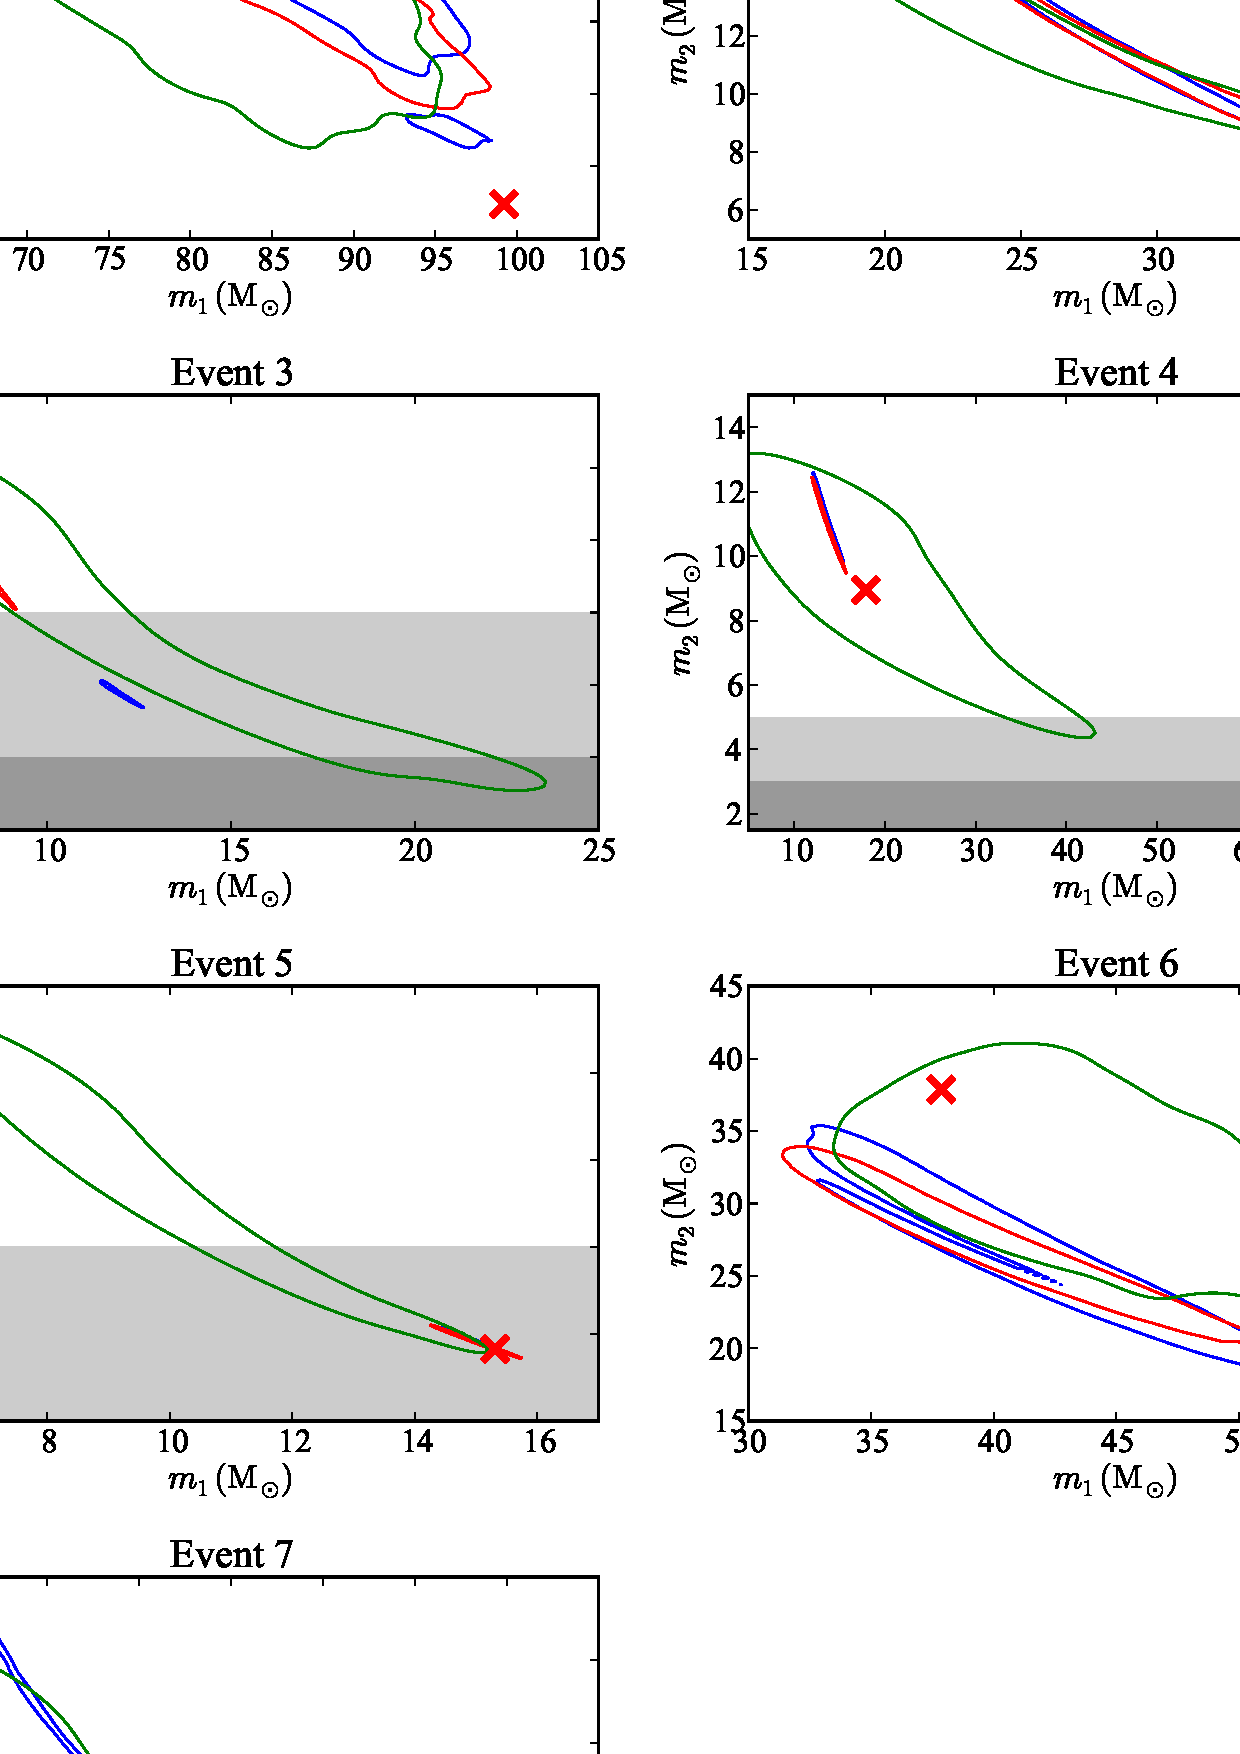
\includegraphics[width=0.45\textwidth]{papers/bns_spin/figure6.pdf}
\caption{\label{fig:asd_comparison} The amplitude spectral density for the aLIGO
zero-detuned high-power design sensitivity (blue solid curve), AdV design sensitivity
(red dashed curve), initial LIGO design sensitivity (blue bot-dash curve) and initial
Virgo design sensitivity (red dotted curve).}
\end{figure}


The process we described above is applicable for any PSD, and therefore we can use it directly
to determine the $\xi_i$ directions for the AdV PSD, or the aLIGO PSD with
a 10Hz lower frequency cutoff. In Figure \ref{fig:param_space_mismatch_alt} we plot
$\xi_1$ against $\xi_2$ for both PSDs while the color shows the mismatch between the center and edges in
the $\xi_3$ direction. This plot can be directly compared to Figure \ref{fig:param_space_mismatch}. We notice
that the size of the parameter space for the AdV PSD is significantly smaller than for the
aLIGO PSD in all 3 of the dominant directions. Therefore our conclusions for aLIGO are still
valid for AdV. Using our method we find that we require approximately 120,000 templates to cover the
parameter space for AdV, in comparison to approximately 520,000 templates for aLIGO. 

By comparing the results when using the aLIGO PSD with a 10Hz and 15Hz lower cut off we observe
that using a 10Hz lower frequency cut off will increase the number of necessary templates from $\sim520000$
to $\sim860000$. However the
shape of the parameter space, and thus our final conclusions, are unaffected when using a 10Hz lower
frequency cutoff. However, in this case we see larger mismatches due to the depth of $\xi_3$ and
therefore the process of stacking templates is important when using a 10Hz lower cut off. However, even
in this case, we do
not feel that the depth is large enough everywhere in the space to justify using a fully 3-dimensional placement
algorithm.

\begin{figure}
\includegraphics[width=0.45\textwidth]{papers/bns_spin/figure7a.png}
\includegraphics[width=0.45\textwidth]{papers/bns_spin/figure7b.png}
\caption{\label{fig:param_space_mismatch_alt} The mismatch between the edge and centre of the
third dominant direction as a function of the first and second dominant
directions when using the Virgo noise curve (top) and when using the advanced LIGO noise curve
with a 10Hz lower frequency cut off (bottom). The $\xi_i$ coordinates have been scaled
such that one unit corresponds to the coverage diameter of a template
at 0.97 mismatch.
Plotted for a binary neutron star parameter space with spins restricted
to 0.4.}
\end{figure}

Finally, we wish to investigate the effect that the higher order spin contributions to the orbital phase
have on our method. To do this we repeat the process described above, but include the spin(1)-spin(1) and
spin(2)-spin(2) contributions to the $\sigma$ term at 2PN order and also the 2.5PN spin-orbit term as given
in \cite{Arun:2008kb}. In Figure \ref{fig:higher_order_spin} we plot $\xi_1$ against $\xi_2$ when these
higher order spin terms are included, the color shows the mismatch between the center and edges
in the $\xi_3$ direction. This plot can be directly compared to Figure \ref{fig:param_space_mismatch}.
By comparing these plots we can see that including the higher order spin terms has caused the parameter space
to have a larger extent in the $\xi_2$ direction. However, the depth of the space in the $\xi_3$ direction
has reduced by almost an order of magnitude. In this case the stacking process is not required and the resulting
bank consists of $\sim560000$ templates. 

\begin{figure}
\includegraphics[width=0.45\textwidth]{papers/bns_spin/figure8.png}
\caption{\label{fig:higher_order_spin} The mismatch between the edge and centre of the
third dominant direction as a function of the first and second dominant
directions using waveforms incorporating the sub-dominant spin corrections to the orbital phase.
The $\xi_i$ coordinates have been scaled
such that one unit corresponds to the coverage diameter of a template
at 0.97 mismatch.
Plotted for a binary neutron star parameter space with spins restricted
to 0.4
using the zero-detuned, high-power aLIGO sensitivity curve with a 15Hz lower frequency cut off.}
\end{figure}

\section{Comparison to alternative placement methods}

An alternative approach to template placement for aligned spin systems is to use templates
with ``unphysical'' values of the symmetric mass ratio, $\eta$.
That is, to use non-spinning templates, with the desired range of chirp
mass but where the range of $\eta$ values is extended to include both values of $\eta$ that are much lower than
the relevant parameter space and values of $\eta$ that are much higher,
including templates with $\eta$ greater than the physically possible limit of 0.25.

We can understand this unphysical $\eta$ approach in terms of our $\xi_i$ coordinate system by noting that
it is always possible to produce a template with any possible value
of $\xi_1$ and $\xi_2$ that is within the BNS parameter space, by using non-spinning templates
with unrestricted values of $\eta$.
By generating a set of templates in the $\xi_1$, $\xi_2$ directions,
where we restrict the chirp mass to be that possible for BNS systems, but where $\eta$
ranges from 0.1 to 0.7 we are able to cover the full physically possible space in $\xi_1$, $\xi_2$. However,
the disadvantage to using unphysical $\eta$ templates is that the points will not take the correct values
of $\xi_3$. The colorbar on Figure \ref{fig:unphys_eta} indicates the mismatch between unphysical $\eta$ templates and
aligned-spin templates as a function of $\xi_1$ and $\xi_2$. In making this plot we assume that $\xi_3$
has no depth in the aligned spin case by taking the central value where $\xi_3$ has a range of values.

While unphysical $\eta$ templates will produce an increase in efficiency when compared with non-spinning templates, the
method is not as efficient as the aligned spin geometrical placement we have described. In addition, both methods
require the same number of templates to cover the parameter space. Therefore, we would recommend using aligned spin templates
placed using our metric algorithm as opposed to unphysical $\eta$ templates.

\begin{figure}
\includegraphics[width=0.45\textwidth]{papers/bns_spin/figure9.png} 
\caption{\label{fig:unphys_eta} The mismatch between unphysical $\eta$ and
aligned spin BNS templates as a function of the first and second dominant
directions. In making this plot we assume that $\xi_3$
has no depth in the aligned spin case by taking the central value where $\xi_3$ has a range of values.
This plot was generated
with spins restricted to 0.4 using the zero-detuned, high-power advanced LIGO
sensitivity curve with a 15Hz lower frequency cut off. 
}
\end{figure}

Finally, we wish to compare the performance of this geometrical algorithm with the stochastic bank proposed in
\cite{Harry:2009ea,Babak:2008rb}. The stochastic placement works by randomly placing points within the parameter
space and rejecting points that are too ``close'' to points already in the bank. This
has the advantage that it is valid for any parameter space metric, so we could use any of the metrics discussed
above. However, it is more computationally efficient to use the Cartesian $\xi_i$ or $\mu_i$ coordinate system
rather than the non-Cartesian metric given above.

The disadvantage to a stochastic bank, when compared to a geometrically placed bank, is that it will require more
templates to achieve the same level of coverage \cite{Harry:2009ea,Manca:2009xw}.
For our parameter space, consisting of BNS signals with
component spins up to 0.4 and using the advanced LIGO zero-detuned high-power design curve with a 15Hz lower
frequency cut-off,
we found that the stochastic placement
produced a bank containing $\sim 750000$ templates, which is 44\% more than with the geometrical placement.
However, stochastic placement can still be used to place templates when no analytical metric is known, such
as when the merger becomes important. In such regions of parameter space, the stochastic placement may still be the best
algorithm to use to place a template bank.

\section{Performance of the aligned spin template bank}
\label{sec:aligned_spin_performance}

In this section we would like to investigate the improvement in the 
detection of generic BNS systems that results from using a template bank
that includes the dominant, non-precessing, spin effects. To do this we use the aligned spinning bank that
we detail in section \ref{sec:param_space} and compare this to the results of using a nonspinning bank 
as shown in section \ref{sec:spin_import}. 

Using our aligned spin template bank, we repeat the investigation from section \ref{sec:spin_import}. We create a 
population of source BNS signals identical to those used in \ref{ssec:nonspin_performance}, and compute the fitting factor
between these signals and the aligned spin template bank. The results of this are shown in FIG.\ref{fig:anstar-prec}.
To decrease the computational cost of this test, we only calculated the overlaps between a signal and templates that
were within a range of $\pm0.1M_{\odot}$ in chirp mass. This is reasonable because the overlap will decrease rapidly
with small changes in chirp mass,
therefore we expect templates with very different values of chirp mass to have low overlaps with each other. We verified
that this approach did not cause us to underestimate the fitting-factor of our banks.

We can now compare the results obtained in this section, using our aligned-spin template bank, with the results obtained in section
\ref{sec:spin_import}, using a non-spinning template bank. One can clearly see an 
improvement in the distribution of fitting factors when using the aligned spin template bank. The fraction
of signals that fall below a fitting factor of 0.97, when the spin magnitudes are restricted to 0.4, falls from 59\% to 9\%.
We also see an  improvement for signals that have spin magnitudes restricted to 0.05, where the fraction of signals falling below a
fitting factor of 0.97 drops from 6\% to 0.2\%. We can also compare the performance of the aligned-spin bank to that of the
non-spinning bank as a function of the maximum spin magnitude,
as shown in Figure \ref{fig:anstar-st-spin}. From this Figure we can see that regardless of the maximum component
spin, the aligned spin bank will greatly reduce the number of signals recovered with fitting factors less than 0.97.

\begin{figure}
\includegraphics[width=0.45\textwidth]{papers/bns_spin/figure10.pdf}
\caption{\label{fig:anstar-prec} The distribution of fitting factors obtained by searching
for the precessing signals described in section \ref{ssec:nonspin_performance}
with component spins up to 0.4 (blue solid line), 0.2 (green dashed line), and 0.05 (red dotted line) using the aligned spin
BNS template bank described in section \ref{sec:param_space} and the advanced LIGO, zero-detuned,
high-power PSD with a 15Hz lower frequency cutoff.}
\end{figure}
% We want to answer: 
% Does the aligned spin work as designed? 
% How well does it work for generic BNS systems?
\begin{figure}
\includegraphics[width=0.45\textwidth]{papers/bns_spin/figure11.pdf}
\caption{\label{fig:anstar-st-spin} The fraction of the precessing signals described in
section \ref{ssec:nonspin_performance} recovered with a fitting factor less than 0.97 as
a function of the maximum component spin. Shown for the non-spinning
BNS template bank described in section \ref{ssec:nonspin_performance} (blue solid line),
and the aligned spin
BNS template bank described in section \ref{sec:param_space} (red dotted line). The advanced LIGO, zero-detuned,
high-power PSD with a 15Hz lower frequency cutoff was used when computing the fitting factors.}
\end{figure}

A small fraction of signals fall below a FF of 0.97, even when using the new aligned-spin template bank.
We expect that these poor matches with the aligned template bank are
due to precession. In general, precessional effects will not be important in BNS systems
as the orbital angular momentum is significantly larger than the component spins.
In such cases there is only a small angle between the total and orbital angular momenta
and precession has only a small effect on the waveform.

However, there is a small region of parameter space where precessional effects \textit{will}
have an effect for BNS systems.
Using the model of Ref.~\cite{Brown:2012gs}, applied to the small precession angles in BNS systems, 
we can predict for which systems precession will be most important.
The orientation of a precessing binary must be defined using the total angular momentum rather than the 
orbital angular momentum as done with non-precessing binaries. 
The orientations with the worst matches should be those where the system is edge-on 
(angular momentum perpendicular to the viewing direction) and where the detector is nearly insensitive 
to the plus polarization and only sees the cross polarization (a binary overhead of the detector would have 
its angular momentum oriented $45^{\circ}$ between the arms of the detector).
We find that
this is indeed the case; in fact, all cases with fitting factors less than 0.95 are close to
this configuration. All of these cases also have biases in the recovered mass and
spin parameters due to the secular effects of precession on the phasing of the waveform.

\section{Conclusion}
\label{sec:conclusion}

In this work we have investigated the effects of neglecting spin when
searching for binary neutron star systems in aLIGO and AdV. We have found
that, if component spins in binary neutron star systems are as large as 0.4,
then neutron star spin cannot be neglected, and there is a non-trivial loss in
signal-to-noise ratio even if the maximum spin is restricted to be less than
0.05.  We have developed a new algorithm for placing an aligned spin template
bank in the BNS parameter space.  We have shown that this bank works for
aligned spin systems and have demonstrated that it does significantly better
for generic, precessing BNS systems than the traditional non-spinning bank.
However, for the BNS aligned spin $\chi_i < 0.4$ parameter space the aligned
spin bank requires approximately five times as many templates as the
non-spinning bank. This increased number of templates will increase the
computational cost of the search and increase the number of background events,
so needs to be balanced against the potential gain in being able to cover a
larger region of parameter space. A further advantage of our method is the ease
with which it can be incorporated into existing or future search
pipelines, which include the use of signal-based vetoes~\cite{Allen:2004gu}
and coincidence algorithms~\cite{Robinson:2008}. In future work we will
investigate how this template bank performs in data from the aLIGO and AdV
detectors which includes non-Gaussian and non-stationary noise features.
Finally we note that the method proposed in this work should be applicable
wherever the TaylorF2 waveforms closely represent actual gravitational
waveforms. In a future work we will investigate how well this method performs
in the binary black hole and neutron-star, black-hole regions of the parameter space.
Wherever the TaylorF2 approximation begins to break down, a stochastic
bank placement may still be the most viable option.

\section*{Acknowledgements}

The authors are greatful to Stefan Ballmer, Stephen Fairhurst, Eliu Huerta, Drew Keppel, Prayush Kumar, Frank Ohme, Ben Owen,
Reinhard Prix, Peter
Saulson, B.S. Sathyaprakash, John Veitch, Matthew West and Karl Wette for helpful discussions. DB, IH and AN are
supported by NSF award PHY-0847611. IH and AN are also also supported by NSF
award PHY-0854812. AL was supported by NSF grant PHY-0855589 and the Max Planck Gesellschaft. DB and IH are also supported by a Cottrell Scholar award
from the Research Corporation for Science Advancement.  Computations used in
this work were performed on the Syracuse University Gravitation and Relativity
cluster, which is supported by NSF awards PHY-1040231, PHY-0600953 and
PHY-1104371.


\Chapter{Accuracy of Post-Newtonian Waveforms for Neutron Star -- Black Hole Searches}
\label{ch:nsbh_faith}
\newcommand\abs[1]{\ensuremath{\left|#1\right|}}

\def\be{\begin{equation}}
\def\ee{\end{equation}}

\def\bea{\begin{eqnarray}}
\def\eea{\end{eqnarray}}

\def\Msun{M_\odot}

\def\cross{\times}


%\eads{\mailto{} \mailto{}}



\acrodef{aLIGO}[aLIGO]{Advanced Laser Interferometer Gravitational-wave Observatory}
\acrodef{AdV}[AdV]{Advanced Virgo}
\acrodef{LIGO}[LIGO]{Laser Interferometer Gravitational-wave Observatory}
\acrodef{CBC}[CBC]{compact binary coalescence}
\acrodef{S6}[S6]{LIGO's sixth science run}
\acrodef{VSR23}[VSR2 and VSR3]{Virgo's second and third science runs}
\acrodef{EM}[EM]{electromagnetic}
\acrodef{NS}[NS]{neutron star}
\acrodef{BH}[BH]{black hole}
\acrodef{BNS}[BNS]{binary neutron star}
\acrodef{NSWD}[NSWD]{neutron star-white dwarf}
\acrodef{NSBH}[NSBH]{neutron star and a black hole}
\acrodef{GRB}[GRB]{gamma-ray burst}
\acrodef{S5}[S5]{LIGO's fifth science run}
\acrodef{S4}[S4]{LIGO's fourth science run}
\acrodef{VSR1}[VSR1]{Virgo's first science run}

\acrodef{PSD}[PSD]{power spectral density}
\acrodef{VSR3}[VSR3]{Virgo's third science run}
\acrodef{BBH}[BBH]{binary black holes}
\acrodef{SNR}[SNR]{signal-to-noise ratio}
\acrodef{SPA}[SPA]{stationary-phase approximation}
\acrodef{LHO}[LHO]{LIGO Hanford Observatory}
\acrodef{LLO}[LLO]{LIGO Livingston Observatory}
\acrodef{LSC}[LSC]{LIGO Scientific Collaboration}
\acrodef{PN}[PN]{post-Newtonian}
\acrodef{DQ}[DQ]{data quality}
\acrodef{IFO}[IFO]{interferometer}
\acrodef{DTF}[DTF]{detection template families}
\acrodef{FAR}[FAR]{false alarm rate}
\acrodef{FAP}[FAP]{false alarm probability}
\acrodef{PTF}[PTF]{physical template family}
\acrodef{ADE}[ADE]{advanced detector era}
\acrodef{FFT}[FFT]{Fast Fourier Transformation}
\acrodef{GPU}[GPU]{graphical processing unit}
\acrodef{ISCO}[ISCO]{inner-most stable circular orbit}
\acrodef{MECO}[MECO]{minimum energy circular orbit}

\section{Introduction}
\label{sec:introduction}

In this paper we investigate if the currently available post-Newtonian models
are sufficient for use in searches for gravitational-waves from the
coalescence of a neutron star and a black hole. Given the uncertainties in the masses and spins of
\ac{NSBH} binaries, we consider a fairly broad mass and spin
distribution when investigating the accuracy of \ac{NSBH} waveforms.
In this paper, we consider \ac{NSBH} binaries with the \ac{NS} mass between 1
and $3\, M_\odot$, the \ac{BH} mass between $3$ and $15\, M_\odot$, the
\ac{NS} spin between 0 and $0.05$ and the
\ac{BH} spin between 0 and 1. Between these limits, the distributions of mass and spin are all
assumed to be uniform. 

Gravitational-wave detectors are sensitive to the phase evolution of the waves radiated
by the binary. \ac{PN} theory can be used to compute the
energy of a compact binary $E(v)$ and the flux radiated in gravitational waves
$\mathcal{F}(v)$ in terms of the invariant velocity $v = (\pi M f)^{1/3}$,
where $M = m_1 + m_2$ is the total mass of the binary, and $f$ is the
gravitational-wave frequency~\cite{Blanchet:2006zz}. By solving the energy
balance equation $dE/dt = - \mathcal{F}$, we can obtain expressions for the
gravitational-wave phase as a function of time $\phi(t)$ or, equivalently, the
Fourier phase of the waves as a function of frequency $\Psi(f)$. At leading
order, the gravitational wave phase depends only on the chirp mass
$\mathcal{M}_c = (m_1 m_2)^{3/5} / (m_1 + m_2)^{1/5}$~\cite{Peters:1963ux}.
Beyond leading order, the waveforms also depend on the symmetric mass
ratio $\eta = m_1 m_2 / (m_1 + m_2)^2$~\cite{Wiseman:1993aj,Blanchet:1995fg,Blanchet:1995ez,Blanchet:1996pi,
Blanchet:2001ax, Blanchet:2004ek}, with spin-orbit 
corrections entering at the third correction beyond leading order~\cite{Kidder:1992fr,
Kidder:1995zr,Arun:2008kb,Blanchet:2012sm,Bohe:2013cla}.

There are several different ways in which to solve the energy balance equation
to obtain the gravitational-wave phase measurable by aLIGO; these different methods are known as
\ac{PN} \emph{approximants.} While the convergence of the full \ac{PN} series 
is not guaranteed, for \ac{BNS} systems in Advanced LIGO, the
available \ac{PN} approximants produce waveforms that are indistinguishable for
a given binary and are reliable for use in detection searches and parameter
measurement~\cite{Simone:1996db,Buonanno:2009zt,Brown:2012qf}. However, for \ac{NSBH}
binaries the total mass, and hence the \ac{PN} expansion parameter $v$, is
larger. The mass ratio and spin corrections are also more significant.
In this paper, we investigate the accuracy of 
waveforms generated by different \ac{PN} approximants for observing \ac{NSBH}
binaries with aLIGO.
To do this, one could compare subsequent terms in the \ac{PN} expansion and
determine the effect of neglecting them. However, in the case of systems whose
component objects are spinning, only terms up to 2.5\ac{PN} order are
completely known~\cite{Kidder:1992fr,Kidder:1995zr,Arun:2008kb}. 
This represents the leading order (1.5\ac{PN}) and
next-to-leading order (2.5\ac{PN}) spin-orbit, along with the leading order
(2.0\ac{PN}) spin-spin contributions to the phasing~\cite{Kidder:1992fr,Kidder:1995zr,Arun:2008kb}.  
We choose to compare approximants that are constructed with terms up to the same
\ac{PN} order, but that use inversely related differential equations to solve
for the orbital dynamics, in addition to comparing to approximants that include
higher order spin-related corrections at partially derived orders~\cite{Bohe:2013cla, Blanchet:2011zv}.
These methods both have the effect of testing
how well the \ac{PN} series has converged. We also present a comparison between
waveforms from these \ac{PN} approximants where we fix the mass and spin
parameters of the objects in order to understand when in the inspiral the waveforms diverge.

We consider two families of \ac{PN} approximants for binaries where the spin
of the black hole is aligned with the orbital angular momentum:
TaylorT2~\cite{Blanchet:1996pi, Droz:1999qx, Blanchet:2006zz} and
TaylorT4~\cite{Buonanno:2002fy}.  In these models, we include all the
completely known orbital evolution terms (up to 3.5\ac{PN} order)~\cite{Wiseman:1993aj,Blanchet:1995fg,Blanchet:1995ez,Blanchet:1996pi,
Blanchet:2001ax, Blanchet:2004ek} and all the
completely known spin-related terms (up to 2.5\ac{PN}
order)~\cite{Faye:2006gx, Blanchet:2006gy, Kidder:1992fr, Mikoczi:2005dn,
Racine:2008kj}.  Restricting to systems where the spin angular momenta are
aligned (or anti-aligned) with the orbital angular momentum means that the
plane of the binary does not precess, simplifying our comparisons. However,
this study captures the dominant effect of spin on the
waveforms~\cite{Brown:2012gs}. In a separate paper, we investigate the effect
of precession on detection searches~\cite{Harry:2013tca}.
We also consider the
effective-one-body model as described in Ref.~\cite{Taracchini:2012ig}. 
We restrict to comparing the inspiral portion of approximants. Even at the upper 
range of masses we consider, $(3+15)M_{\odot}$, it has been shown in the case of numerically modelled 
binary black hole waveforms that inspiral-only
template banks recover $> 95\%$ of the signal power~\cite{Brown:2012nn, Smith:2013mfa}.
We separately consider models that include
spin-related terms up to 3.5\ac{PN} order~\cite{Bohe:2013cla,
Blanchet:2011zv}. Spin-orbit tail (3.0\ac{PN}) and next-to-next-to-leading
order spin-orbit (3.5\ac{PN}) contributions to the phasing are known.
However, these orders are incomplete as there are also unknown spin
corrections at 3.0\ac{PN} and 3.5\ac{PN}, including spin-spin and
(spin-induced) octupole-monopole couplings. 

In Fig.~\ref{fig:t4horizon} we show  
the distance an optimally oriented system would be observed at \ac{SNR} 8 (the horizon distance),
for a $1.4\Msun-10\Msun$ \ac{NSBH} system, as a function of the spin of the
black hole, for both the \ac{aLIGO} zero-detuned, high-power sensitivity curve and a
plausible range of early \ac{aLIGO} sensitivities~\cite{Aasi:2013wya}. 
Systems where the spin of the black hole is large in magnitude and aligned with the orbital 
angular momentum can be seen from a greater distance than systems where the spin is 
small or anti-aligned. Achieving this sensitivity requires \ac{NSBH} waveforms that do not
incur a significant loss in \ac{SNR} when used as search templates ~\cite{Apostolatos:1996rf}.
Furthermore, extracting the physics from observed signals requires faithful templates for parameter measurement.

We find that no presently available waveform model is sufficiently accurate for use
in \ac{aLIGO} \ac{NSBH} searches or parameter measurement. Our key results, Figs.~\ref{fig:f2f4f}-\ref{fig:seobnrf},
show the match between the various waveform families considered here.
There is a significant disagreement between the \ac{PN} approximants we
have examined, even at at low ($\chi \sim 0.4$) spins and small ($m_{BH}/m_{NS} \sim 4$) mass ratios for TaylorF2 and TaylorT4.
The match decreases as these increase with matches as low as $\sim 0.1$ observed. This motivates
the need to compute higher order \ac{PN} spin corrections.  

Our present knowledge of \ac{NSBH} waveforms will limit the
ability of gravitational-wave observatories to accurately determine source
parameters from the detected signals and may hinder their detection.
Further analytical and numerical modeling of \ac{NSBH} systems will be needed
before \ac{aLIGO} comes online in 2015 and reaches full sensitivity in $\sim$
2019~\cite{Aasi:2013wya}.

The remainder of this paper is organized as follows.  In
Sec.~\ref{sec:waveforms}, we describe the construction of the \ac{PN}
approximants used and Sec.~\ref{sec:faithfulness_definition} describes our
method of comparing them.  In Sec.~\ref{sec:faithfulness} we show the results
of comparing different \ac{PN} approximants, and show that there is a large
discrepancy between the waveforms for \ac{NSBH} binaries at relatively low
black hole spins. In Sec.~\ref{sec:R2F4} we construct a new frequency domain
approximant that is designed to agree with TaylorT4. This is followed by a
comparison of the time domain approximants to their frequency domain
counterparts in Sec.~\ref{sec:freq_vs_time_approx}, where we demonstrate that
they largely agree. Finally, in Sec.~\ref{sec:faithfulness_phase} and
Sec.~\ref{sec:faithfulness_match_accumulation} we investigate where in the
inspiral the disagreement between the waveform families becomes important. We
demonstrate that the divergence occurs at surprisingly low velocities for even
modest black hole spins. Finally in Sec.~\ref{sec:effectualness_and_flow} we
investigate whether maximizing over the mass and spin parameters of the
waveform can improve present models, and investigate the accuracy of the
waveforms for early aLIGO observations when the detectors will have reduced
low-frequency sensitivity when compared to the ultimate sensitivity. 

%%%%%%%%%
%\section{Observational Mass and Spin Distributions}
%\label{sec:dist}


\begin{figure}
\begin{center}
\includegraphics{papers/nsbh_faithfulness/figure1.png}
\end{center}
\caption{\label{fig:t4horizon} 
The horizon distance as a function of the spin of the black hole 
for a $1.4\Msun-10\Msun$ \ac{NSBH} system, for both the \ac{aLIGO} zero-detuned,
high-power aLIGO sensitivity curve (blue) and plausible early \ac{aLIGO}
detector sensitivities (red), with a 15 Hz lower frequency cutoff. 
Results are obtained using the TaylorT4 approximant including only the 
complete spin terms up to 2.5\ac{PN}. Note that \ac{aLIGO} will be sensitive to
\ac{NSBH} systems out to $\sim 900$ Mpc, and there will be increased sensitivity
for systems with aligned black hole spins with large magnitudes. 
}
\end{figure}


%%%%%%%%
\section{Post-Newtonian approximant faithfulness comparison}
\label{sec:faithfulness}

\begin{figure}
\begin{center}
\includegraphics{papers/nsbh_faithfulness/figure2.png}
\end{center}
\caption{\label{fig:f2f4f}The match between the TaylorF2 and
TaylorT4 approximants as a function of the spin of the black hole
and the mass ratio of the system. Only the completely known 
spin-related corrections up to 2.5\ac{PN} are included. Matches are calculated using the
the aLIGO zero-detuned, high-power sensitivity curve and a 15Hz lower frequency cutoff.
A significant reduction in match is seen for even moderate spins $\chi \sim 0.3$
and low mass ratios $m_{bh}/m_{ns} \sim 4$. The approximants also begin to disagree for non-spinning
systems as the mass ratio increases.
}


\end{figure}

\begin{figure}
\begin{center}
\includegraphics{papers/nsbh_faithfulness/figure3.png}
\end{center}
\caption{\label{fig:f2t4fso}The match between the TaylorF2 and TaylorT4 approximants
as a function of black hole spin and mass ratio. Both models include
the next-to-next-to-leading spin-orbit (3.5\ac{PN}) and spin-orbit tail 
terms (3.0\ac{PN}). In comparison to Fig. \ref{fig:f2f4f}, the additional terms have 
improved the agreement for moderately spinning aligned spin systems, however, the
match is still $ \sim 0.8 $ for $\chi \sim 0.5 $ at all mass ratios.}

\end{figure}

Searches for gravitational waves from compact binary coalescences utilize
matched-filtering~\cite{Wainstein,Allen:2005fk}, in which the signal model is
correlated with the detector output to construct a signal-to-noise
ratio. If the signal model does not accurately capture the true gravitational
waveform, then the signal-to-noise ratio, and hence the distance to which the
detector can see signals at a given false alarm rate, will decrease. Matched-filtering 
therefore relies on the accuracy of the models. We quantify the 
agreement between waveform families by computing the match, or
\emph{faithfulness} of the waveforms.

The \emph{faithfulness} of representing a waveform from a given \ac{PN} family with
that of another is described by the match between the two waveforms when the
same physical parameters are used as input to the models. As both models
describe the same physical source, the match should be unity. Any deviation is
due to the variation between models and the match gives the fractional loss in
signal-to-noise ratio that will result.

In this section we compare the faithfulness between waveforms from different
\ac{PN} approximants where we choose the physical parameters to be consistent
with \ac{NSBH} sources.  We also consider how the waveforms from the \ac{PN}
approximants compare to the waveforms from the SEOBNRv1 effective-one-body
model~\cite{Taracchini:2012ig}. Lastly, we consider the effect of including 
the spin-related terms at only partially derived orders. 
We model the sensitivity of second generation  gravitational-wave detectors with the aLIGO
zero-detuned, high-power sensitivity curve~\cite{aLIGOSensCurves}. For this
study we use a lower frequency cutoff of 15Hz since it is not expected that
detectors will have significant sensitivity below this frequency. We consider
the effect of increasing this low-frequency cutoff to simulate early aLIGO
sensitivities in Sec.~\ref{sec:effectualness_and_flow}.

In Fig.~\ref{fig:f2f4f}, we examine the faithfulness of \ac{NSBH} waveforms by computing the match between the TaylorF2 and TaylorT4 \ac{PN} approximants.
The TaylorT4 approximant was used to simulate \ac{NSBH} binaries in LIGO's
previous gravitational-wave searches, and the TaylorF2 family is used as the
templates for detection~\cite{Abadie:2011nz}.
In order to focus
on the mismatches primarily due to phase differences between the models, the
frequency cutoff of the TaylorF2 waveform is made to agree with the ending
frequency of the TaylorT4 waveform. We see that the agreement between the two
models is primarily influenced by the magnitude of the black hole's spin, and
secondarily by the mass ratio. There is a noticeable drop in match at higher
mass ratios, even when
the spin of the black hole is zero. As expected, the best
agreement is seen when the black hole's spin is small and
the black hole and neutron star have comparable masses.
However, this plot shows that there is a \emph{substantial} disagreement between
these approximants for even moderately low black hole spins ($\chi \sim 0.3$),
which increases as the spin of the black hole increases. 
We note that the effect on the match due to the spin of the
neutron star is negligible in all areas.  In Fig.~\ref{fig:f2t4fso} we compare
the TaylorF2 and TaylorT4 models, with the inclusion of the spin-orbit
tail (3.0\ac{PN}) and next-to-next-to-leading spin-orbit (3.5\ac{PN})
corrections recently computed in Refs.~\cite{Bohe:2012mr, Blanchet:2012sm}.  In comparison to
Fig.~\ref{fig:f2f4f}, the agreement is improved for aligned spins
with moderate magnitudes. However, these approximants maintain a poor level of
overall agreement, with matches of only $\sim 0.8$ at $\chi \sim 0.5$ for all mass ratios, and even
lower matches for anti-aligned systems. 
Figs.~\ref{fig:5715f2f2} and~\ref{fig:5715t4t4} compare the TaylorT2 and TaylorT4 approximants with and without
these additional spin terms.
We see that TaylorT4 is especially sensitive to the additional corrections.
In both cases, however, we note that the additional terms have caused a significant change in the waveforms, 
as indicated by the low matches, demonstrating that the expansion has
not yet sufficiently converged to produce reliable waveforms for parameter estimation. 

\begin{figure}
\begin{center}
\includegraphics{papers/nsbh_faithfulness/figure4.png}
\end{center}
\caption{\label{fig:5715f2f2}The match between TaylorF2 with 2.5\ac{PN} spin corrections
and TaylorF2 including the next-to-next-to-leading spin-orbit (3.5\ac{PN}) and spin-orbit tail 
terms (3.0\ac{PN}), as a function of the spin of the black hole
and the mass ratio of the system. Matches are calculated using the the aLIGO
zero-detuned, high-power sensitivity curve and a 15Hz lower frequency cutoff. Although 
there is agreement where the spins are low $\chi < 0.2 $, the match quickly drops
as the spin of the black hole increases, so that the match is already $ \sim 0.7 $ for $\chi \sim 0.5$.
}
\end{figure}

\begin{figure}
\begin{center}
\includegraphics{papers/nsbh_faithfulness/figure5.png}
\end{center}
\caption{\label{fig:5715t4t4}The match between TaylorT4  with 2.5\ac{PN} spin corrections
and TaylorT4 including the next-to-next-to-leading spin-orbit (3.5\ac{PN}) and spin-orbit tail 
terms (3.0\ac{PN}), as a function of the spin of the black hole
and the mass ratio of the system. Matches are calculated using the the aLIGO
zero-detuned, high-power sensitivity curve and a 15Hz lower frequency cutoff. 
In comparison to Fig.~\ref{fig:5715f2f2}, the approximant is more noticeably changed
by the additional terms. For a mass ratio of 8, the match has already 
fallen to  $ \sim 0.7 $ for $\chi \sim 0.15$. }
\end{figure}

\begin{figure*}
\begin{minipage}[l]{\columnwidth}
\includegraphics{papers/nsbh_faithfulness/figure6A.png}
\includegraphics{papers/nsbh_faithfulness/figure6B.png}
\caption{\label{fig:seobnrf}The match between the TaylorF2
(left) or TaylorT4 (right) and SEOBNRv1
approximants. Spin corrections for the \ac{PN} approximants are included up to 2.5\ac{PN}.
Matches are calculated using the the aLIGO zero-detuned, high-power sensitivity curve
with a 15 Hz lower frequency cutoff. As in Fig.~\ref{fig:f2f4f}, 
there is a significant reduction in match where
spin of the black hole is only moderate. Note, however, that the
\ac{PN} approximants have marginally better agreement with SEOBNRv1 than with each other.}
\end{minipage}
\end{figure*}


In Fig.~\ref{fig:seobnrf} we compare the SEOBNRv1 model to the \ac{PN} models
TaylorF2 and TaylorT4.  Since the SEOBNRv1 model is not valid
for large values of $\chi$~\cite{Taracchini:2012ig} we restrict
$\chi < 0.6$ and only report matches below this limit.  We see that,
similar to the comparison between TaylorF2 and TaylorT4, these models also have
large mismatches when the spin of the black hole is nonzero.
The large discrepancy between the waveform families indicates that higher order
\ac{PN} correction terms are required. This may also pose significant problems
for parameter estimation of \ac{NSBH} sources.



% We can perhaps argue that we are including only a few comparisons with the 3.5pN NNLO SO as 
% The 3.0 and 3.5pN spin contributions are only incompletely known. There will be additional terms,
% of as yet unkown importance due to the next SS effects, Q-M, and I think some other effects. 
% Perhaps this should be introduced earlier?



%What does sufficient mean in this context?

%%%%%%%%
\section{The TaylorR2F4 approximant}
\label{sec:R2F4}

In the previous section, we found a surprisingly large disagreement between the TaylorF2 and TaylorT4
\ac{PN} approximants when compared with waveform parameters appropriate for
\ac{NSBH} systems. We would like to distinguish how much of this is due to
differences between time domain and frequency domain approximants, and how much
of this is due to differences between the formulation of the two \ac{PN}
families.  This can easily be performed for the TaylorF2 and TaylorT2
approximants, however we need to construct an equivalent frequency domain
version of TaylorT4 to complete the comparison.

By analogy with TaylorF1 and TaylorF2~\cite{Damour:2000zb,Buonanno:2009zt},
TaylorF4 is obtained by numerically integrating the reciprocal of Eq.~\eqref{eq:t4}
in the frequency domain,
%
\begin{equation}\label{eq:f4}
%
dt/dv = 1 / A_k(v).
%
\end{equation}
%
However, this does not elucidate the differences between the TaylorT4 and
TaylorF2 approximants. Instead, we construct an analytical approximation to the
TaylorF4 approximant, which we call TaylorR2F4, by expanding Eq.~\eqref{eq:f4} in
powers of $v$. In order to make this series finite, we truncate these
additional terms at an order in $v$ higher than the order where the \ac{PN}
expansion of the energy and flux were truncated,
%
\begin{equation}
%
\frac{dt}{dv} = \left[ \frac{1}{A_{k}(v)} \right]_l = B_{k}(v) + R_{kl}(v) =
C_{kl}(v).
%
\end{equation}
%
Here $B_{k}(v)$ is the same as in the TaylorT2 approximant and $R_{kl}(v)$ are
the terms from order $v^{k+1}$ up to order $v^l$. It is important to note that
this produces a power series that is identical to the TaylorF2 approximant up
to the point where~\eqref{eq:t2} was truncated.  Thus, terms of higher order in
$v$ account for the differences between the TaylorT2 and TaylorT4 approximants.

In sec.~\ref{sec:freq_vs_time_approx} we show that TaylorR2F4 agrees well with the TaylorT4 approximant
when expanded to $v^9$ or $v^{12}$, which we shall see in the next section.  As
noted above, the second expansion in the TaylorR2F4 approximant is a different
expansion than the \ac{PN} expansion of the energy and flux.  The Fourier phase
for the TaylorR2F4 approximant can be obtained from~\eqref{eq:phaset2}  where
$B_{k}(v)$ is replaced by $C_{kl}(v)$.  This is given up to order $v^N$ as
%
\begin{equation}
%
\psi_{\mathrm{R2F4}}(f) = \psi_{F2}(f) + \sum_{i=6}^{N} \sum_{j=0}^{N}
\lambda_{i, j} f^{(i-5)/3} \log^j f,
%
\end{equation}
%
where the form of these expressions up to $N=12$ can be found in
Appendix~\ref{app:R2F4}.
Because this approximant can be analytically expressed in the frequency domain,
it can be generated relatively cheaply compared to TaylorT4. This means that it has
the potential to be used where computational efficiency and 
a higher degree of agreement with TaylorT4 is desired.
We note that the frequency-domain approximants are much faster than their
time-domain counterparts, which must integrate differential equations and perform 
a Fourier transform. Therefore, they are especially useful in computational problems 
which are waveform-generation limited, 
such as parameter estimation of signals~\cite{Aasi:2013jjl}.

%%%%%%%%
\section{Comparison of Frequency to Time Domain Approximants}
\label{sec:freq_vs_time_approx}

\begin{figure}
\begin{center}
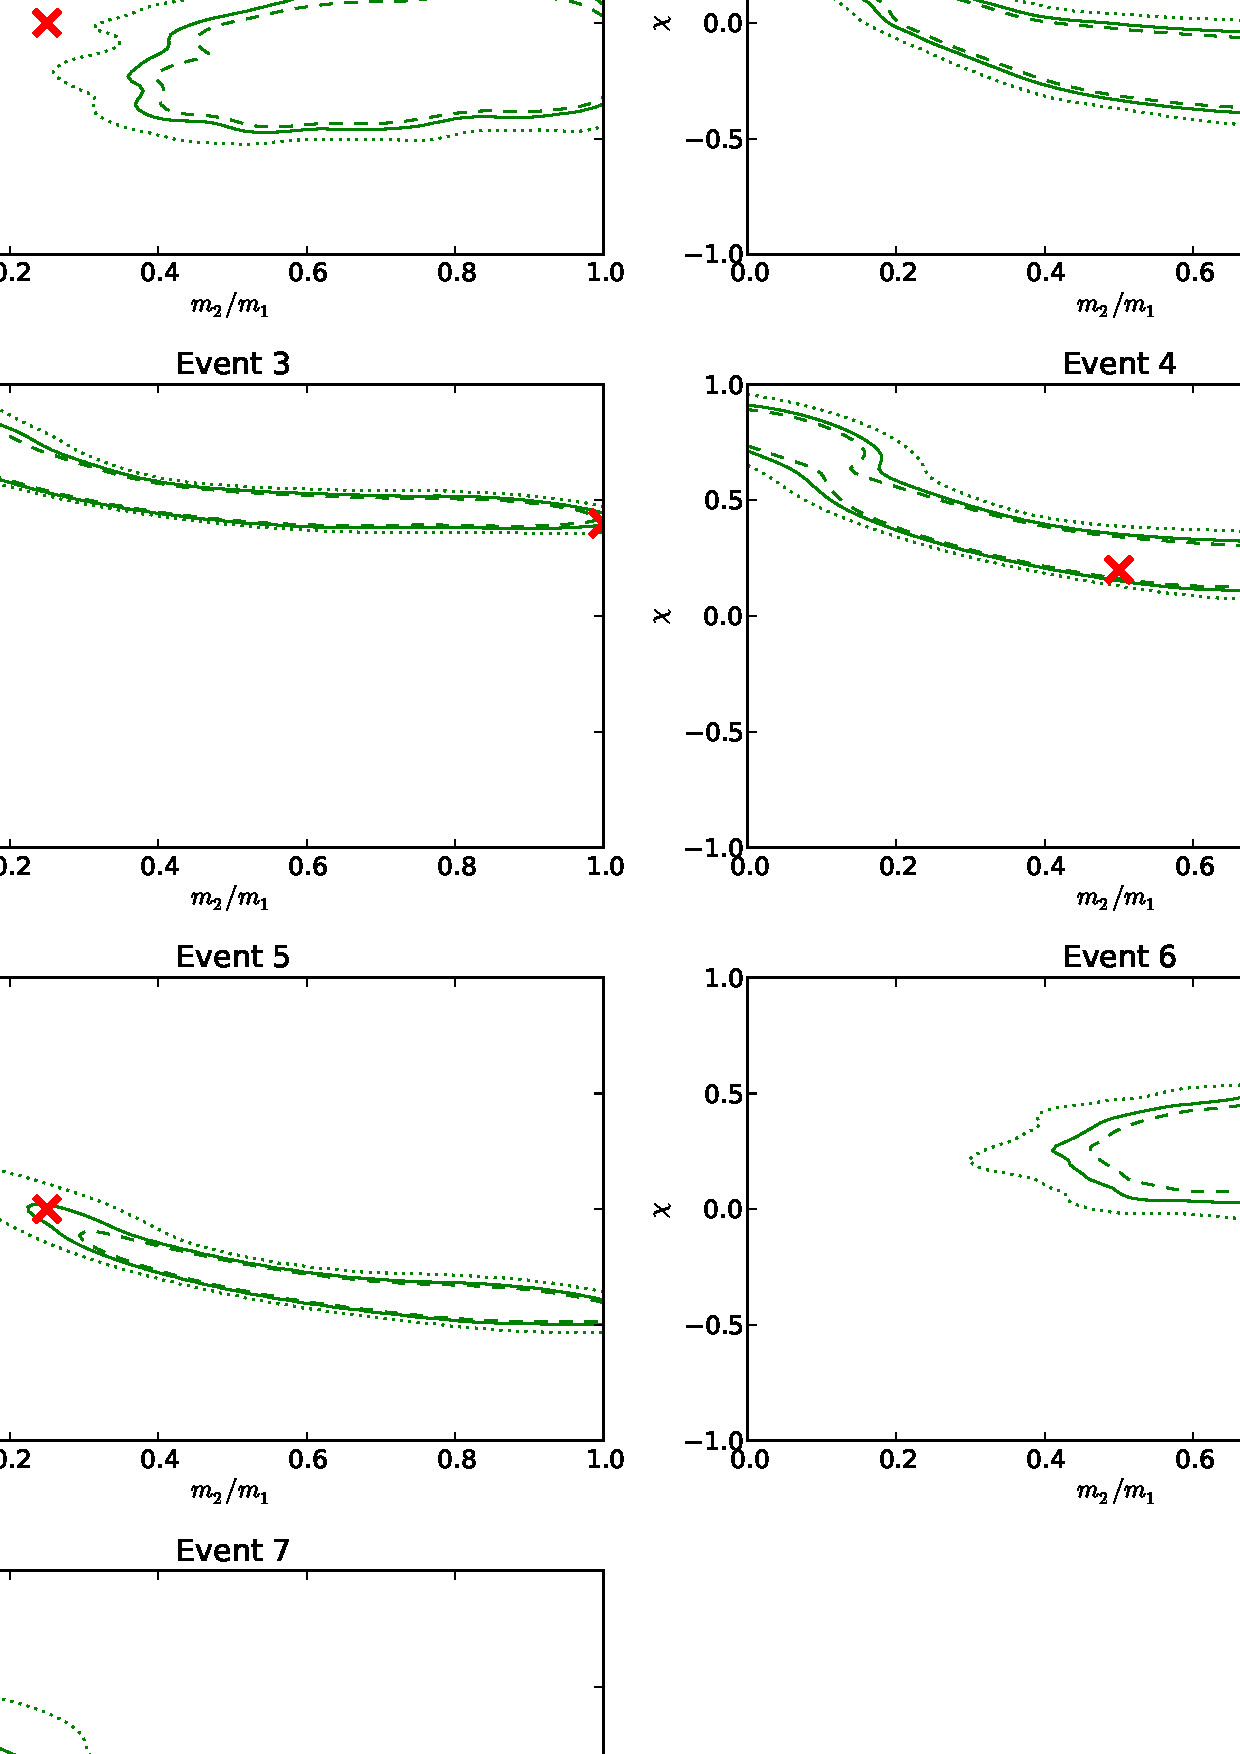
\includegraphics{papers/nsbh_faithfulness/figure7.png}
\end{center}
\caption{\label{fig:f2t2fs} The match between TaylorF2 and TaylorT2. Both include spin 
corrections up to 2.5\ac{PN} order.
Matches are calculated using the the aLIGO
zero-detuned, high-power sensitivity curve and a 15Hz lower frequency cutoff. 
We see that the F2 and T2 approximants largely agree. The discrepancy
between the two approixmants can be reduced by expanding the frequency sweep of
the TaylorF2 approximant's amplitude to higher \ac{PN} orders. However, there
is different Gibbs phenomena between the two approximants that will cause a
discrepancy.}

\end{figure}


\begin{figure*}
\begin{minipage}[l]{\columnwidth}
\includegraphics{papers/nsbh_faithfulness/figure8A.png}
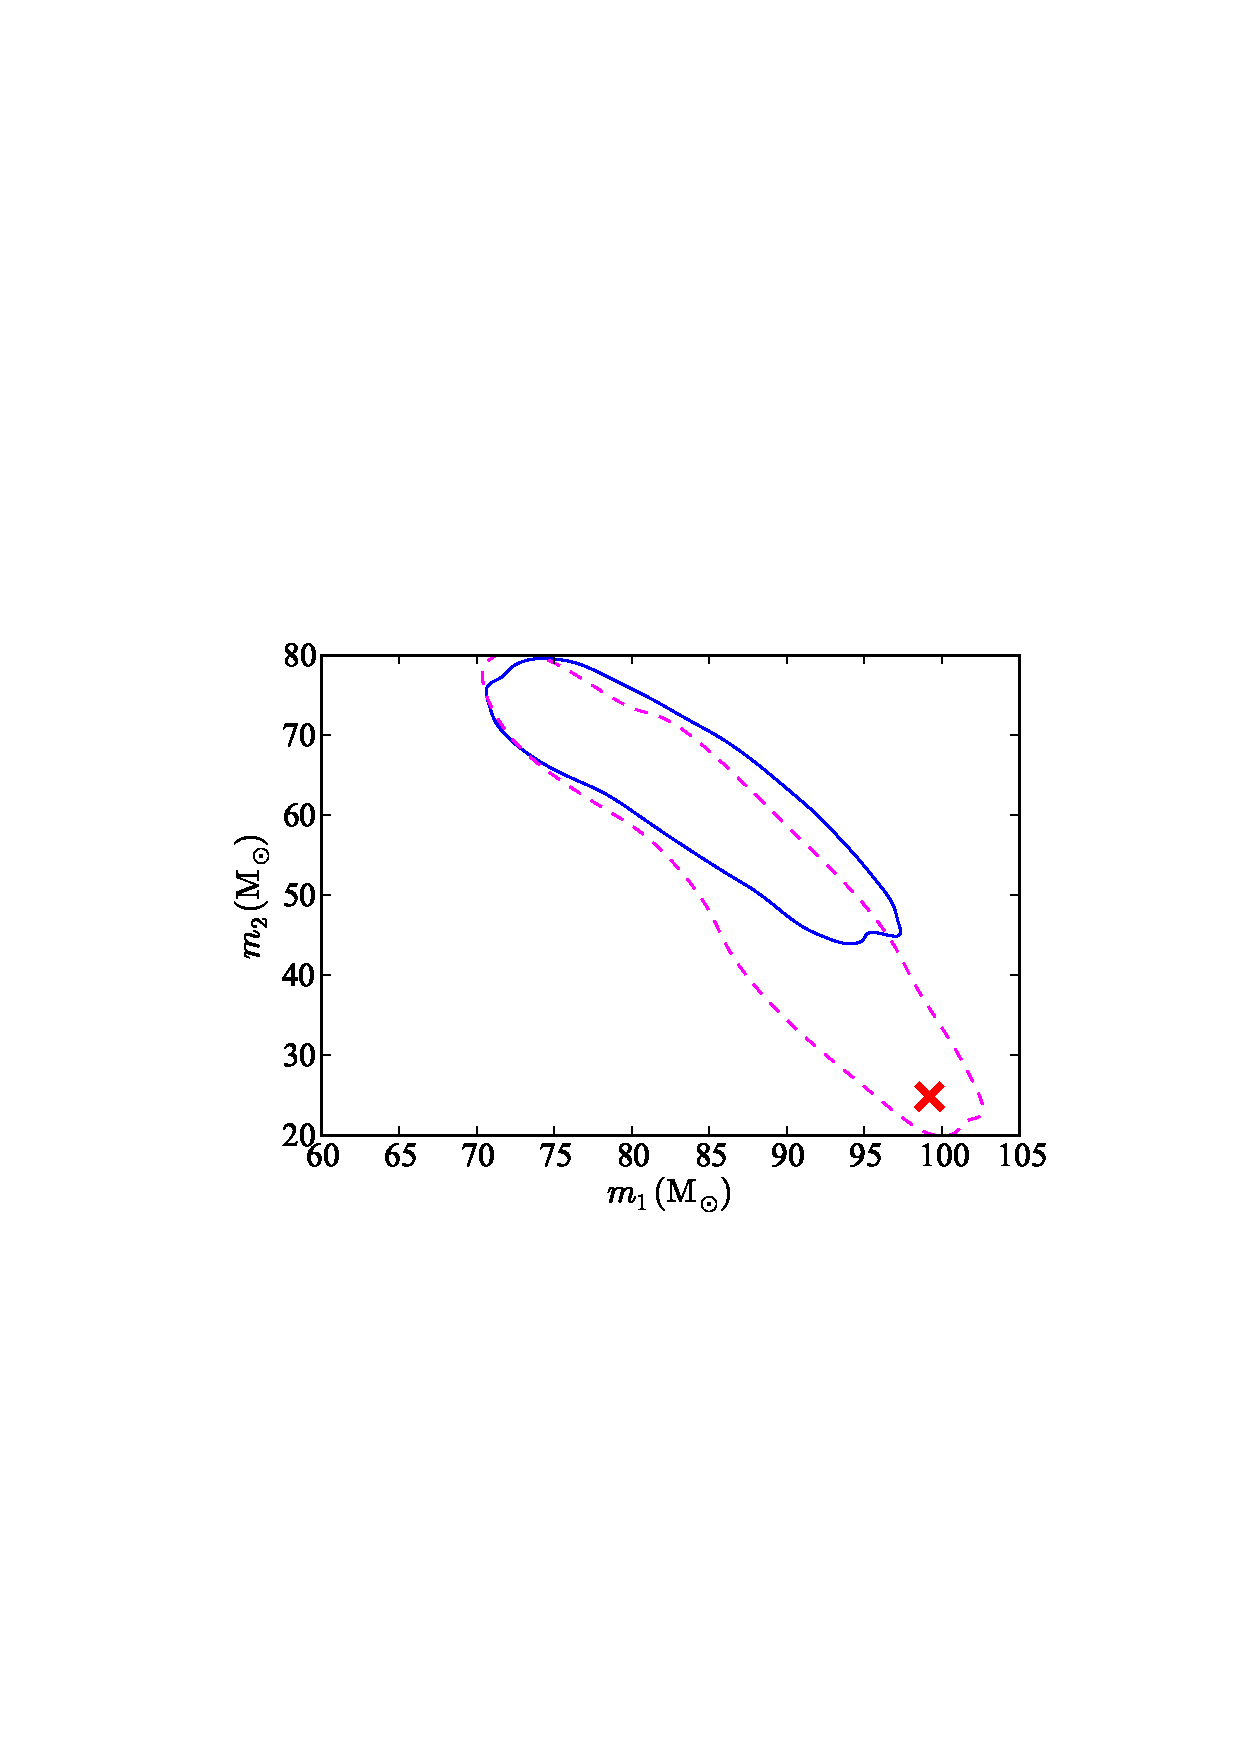
\includegraphics{papers/nsbh_faithfulness/figure8B.png}
\caption{\label{fig:f4t4fs}The match between TaylorT4 and TaylorR2F4. Both models include
spin corrections up to 2.5 \ac{PN}. TaylorR2F4 is  re-expanded up to order $v^9$ (left) 
and $v^{12}$ (right). Matches are calculated using the the aLIGO
zero-detuned, high-power sensitivity curve and a 15Hz lower frequency cutoff. R2F4 and T4 have
high agreement over a broad range of parameters, with some visible exceptions.
Expanding up to order $v^{12}$ has generally increased
agreement with TaylorT4. }
\end{minipage}
\end{figure*}
In this section, we investigate to what extent the discrepancy between the waveform families that
was demonstrated in Sec.~\ref{sec:faithfulness} is due to the difference
between expressing approximants in the frequency and time domain alone.
We compare the new TaylorR2F4 approximant from
Sec.~\ref{sec:R2F4}, and TaylorF2, to their time domain equivalents.


We find that TaylorF2 waveforms are a good representation of
TaylorT2 waveforms, even when we consider waveforms from \ac{NSBH} systems
where the component objects are spinning. This can be seen in
Figure~\ref{fig:f2t2fs}, which shows the match between the TaylorF2 and
TaylorT2 models. In that figure, the ending frequency of both models is made to
be the same, which is accomplished by terminating the TaylorF2 waveforms at the
frequency where the generation of the equivalent TaylorT2 waveforms terminated.
We find that the TaylorF2 and TaylorT2 waveforms agree to better than $\gtrsim
95.7\%$ for the entire region investigated. For systems where the black hole
spin was positively aligned with the orbital angular momentum, the match is
$\gtrsim 97.9\%$. The discrepancy between these two models is in part due to
expanding to only Newtonian order the frequency sweep associated with the
stationary phase approximation of the TaylorF2 approximant. In addition, part
of the discrepancy results from Gibbs phenomena differences between the
approximants.
It is important to note that neither of these waveforms have termination
conditions that are determined by the physical behavior of the inspiralling
binary. The termination frequency only indicates the point at which the
approximant is certainly no longer valid. The increased match for aligned spin
waveforms is due to the higher frequency cutoff, which pushes the termination
frequency out of the most sensitive part of the zero-detuned, high-power aLIGO
sensitivity curve.

Figure~\ref{fig:f4t4fs} shows a comparison between the TaylorR2F4 and TaylorT4
models. In that figure, the second expansion associated with the TaylorR2F4
model is extended to order $v^{9}$ (left) and $v^{12}$ (right), and the ending frequency of both
is that corresponding to the \ac{MECO}.  We show that the TaylorR2F4 model is
adequate for a large range of parameters as a computationally inexpensive
substitute for TaylorT4. 

Since the mismatch between the TaylorF2 and TaylorT4 models is not due to
differences between the time domain and frequency domain approximants, this
indicates that the effective higher order \ac{PN} terms used in the
construction of TaylorR2F4, which are also intrinsically present in TaylorT4,
are still significant. To obtain better agreement between the
different \ac{PN} approximants we consider, it is necessary to extend the
\ac{PN} expansions of the energy and flux equations to include 
unknown higher order terms, particularly ones that involve 
the spin of the objects. 

%%%%%%%%
\section{Accumulation of Phase Discrepancy}
\label{sec:faithfulness_phase}

\begin{figure*}
\begin{center}
\includegraphics[]{papers/nsbh_faithfulness/figure9.pdf}
\end{center}
\caption{\label{fig:T2T4pa} The accumulation of phase differences between
TaylorT2 and TaylorT4, for systems with component masses $(m_1, m_2)$ of
$(1.4\Msun, 6\Msun)$ (left), $(1.4\Msun, 10\Msun)$ (center), and $(1.4\Msun,
14\Msun)$ (right). The approximants include spin terms up to 2.5\ac{PN}.
The calculation starts from the velocity corresponding to a
 gravitational-wave  frequency of $15$Hz, continues to the velocity on the horizontal axis,
and reports the difference in accumulated gravitational-wave phase between the waveforms. The feature
in the bottom right corner of each plot arises because the TaylorT2 approximant is no longer monotonic.
Note that large phase differences accumulate at very low velocities $v \sim 0.2 $
for even small black hole spins.}

\end{figure*}

\begin{figure*}
\begin{center}
\includegraphics[]{papers/nsbh_faithfulness/figure10.pdf}
\end{center}
\caption{\label{fig:T2SEpa} The accumulation of phase difference between
TaylorT2 and SEOBNRv1, for systems with component masses $(m_1, m_2)$ of
$(6\Msun, 1.4\Msun)$ (left), $(10\Msun, 1.4\Msun)$ (center), and $(14\Msun,
1.4\Msun)$ (right). TaylorT2 includes spin terms up to 2.5\ac{PN}.
The calculation starts from the velocity corresponding to a gravitational-wave  frequency of $15$Hz, 
continues to the velocity on the horizontal axis,
and reports the difference in accumulated gravitational-wave phase between the waveforms. The feature
in the bottom right corner of each plot arises because the TaylorT2 approximant is no longer monotonic.
As in Fig.~\ref{fig:T2T4pa}, a large phase difference is
accumulated at low velocities and small black hole spins.}

\end{figure*}


In the previous sections, we demonstrated that the two \ac{PN} approximants,
TaylorF2 and TaylorT4, and the SEOBNRv1 model are not faithful to each other.
We also showed that this is not due to the differences between frequency and
time domain waveforms.  From the construction of the TaylorR2F4 approximant, we
also demonstrated that the two \ac{PN} families can be written in a way that is
consistent up to the chosen \ac{PN} order, but where TaylorR2F4 contains higher
order in $v$ corrections that account for the differences between the models.
Since these are higher order corrections, they should start to become important
to the orbital phasing only at high velocities, and thus high  gravitational-wave 
frequencies. In this section we investigate where, for systems with parameters
corresponding to \ac{NSBH} binaries, the approximants diverge. We do this by
examining the accumulation of phase as a function of orbital velocity and
reporting the difference in the number of  gravitational-wave  cycles between different
approximants.

In Fig.~\ref{fig:T2T4pa}, we examine the difference in the accumulated phase
between TaylorT2 and TaylorT4 for three example systems with component masses
$(m_1, m_2)$ of $(6\Msun, 1.4\Msun)$, $(10\Msun, 1.4\Msun)$, and $(14\Msun,
1.4\Msun)$. We see that the phase difference between the two models quickly
grows to tens of radians, even when the black hole spin magnitude is small.
This is also true when comparing TaylorT2 and SEOBNRv1, as can be seen in
Fig.~\ref{fig:T2SEpa}.  In the latter case, there is also a noticeable
deviation away from the line of zero spin where for unknown reasons the two
models diverge and subsequently converge.

%%%%%%%%
\section{Accumulation of mismatch}
\label{sec:faithfulness_match_accumulation}

\begin{figure*}
\begin{center}
\includegraphics[]{papers/nsbh_faithfulness/figure11.pdf}
\end{center}
\caption{\label{fig:F2T4ma} The match between TaylorF2 and TaylorT4
integrated from 15 Hz up to the designated frequency for systems with component
masses $(m_1, m_2)$ of $(1.4\Msun, 6\Msun)$ (left), $(1.4\Msun, 10\Msun)$
(center), and $(1.4\Msun, 14\Msun)$ (right).  Both approximants include spin corrections up to 2.5\ac{PN}.
Matches are calculated using the the aLIGO
zero-detuned, high-power sensitivity curve. A contour at a match of 0.97 is
indicated by the dotted line.  The match follows the general features seen in
the phase difference comparison of Fig.~\ref{fig:T2T4pa} and drops
significantly, even at relatively low velocities. For the $(1.4\Msun, 6\Msun)$ system with a black
hole spin $\chi = 0.5 $, the match has already dropped to $\sim 0.5$ at a velocity of only $\sim 0.25$.
}
\end{figure*}


\begin{figure*}
\begin{center}
\includegraphics[]{papers/nsbh_faithfulness/figure12.pdf}
\end{center}
\caption{\label{fig:F2SEma} The match between the TaylorF2 and SEOBNRv1 models
integrated from 15 Hz up to the designated frequency for systems with component
masses $(m_1, m_2)$ of $(6\Msun, 1.4\Msun)$ (left), $(10\Msun, 1.4\Msun)$
(center), and $(14\Msun, 1.4\Msun)$ (right). TaylorF2 includes spin corrections up to 2.5\ac{PN}.
Matches are calculated using the the aLIGO
zero-detuned, high-power sensitivity curve. A contour at a match of 0.97 is
indicated by the dotted line. We note that, although the match is marginally
improved compared to Fig.~\ref{fig:F2T4ma}, there are still large
disagreements at velocities as low as 0.25.}

\end{figure*}


As  gravitational-wave  detectors are not directly sensitive to phase differences alone, it
is useful to compute how the match, which incorporates the sensitivity of a
 gravitational-wave  detector, changes as a function of the upper frequency cutoff used for
the calculation. In this section we demonstrate at which frequencies and
corresponding velocities the match between waveform families drops. To do so,
we define an inner product between waveforms that is a function of the upper
frequency cutoff. This inner product is then used in the match calculation of
Eq.~\eqref{eq:match}.

In Fig.~\ref{fig:F2T4ma}, we examine the match between TaylorF2 and TaylorT4,
integrated from a lower frequency cutoff of 15 Hz up to the upper frequency
cutoff indicated on the horizontal axis. This is compared for the same three
example systems as in Sec.~\ref{sec:faithfulness_phase}. The match is shown
across the range of allowable values of the black hole spin and the neutron
star spin is set to zero. We see that the match drops precipitously even at low
velocities and relatively modest spin magnitudes. For example, for a system
with $m_1=6\Msun$, $m_2=1.4\Msun$, and a dimensionless spin of 0.5 for the
black hole, the match drops below 0.7 at a velocity of only 0.23. The loss in
match is more pronounced with increasing mass ratio. 

In Fig.~\ref{fig:F2SEma}, we examine the match between TaylorF2 and SEOBNRv1,
integrated from a lower frequency cutoff of 15Hz up to the upper frequency
cutoff indicated on the horizontal axis. Again, the match drops for large spin
magnitudes at relatively low velocities, although, just as the TaylorF2
approximant has shown better matches with the SEOBNRv1 approximant than with
the TaylorT4 approximant, this occurs at somewhat higher velocities. This shows
clearly that significant portions of the loss in match seen in
Sec.~\ref{sec:faithfulness} occurs at unexpectedly low velocities.


\section{Detection searches and Early aLIGO}
\label{sec:effectualness_and_flow}

In the previous sections, we have demonstrated a substantial loss in match between
different \ac{PN} and EOB models of \ac{NSBH} binaries. These discrepancies
will cause substantial biases in attempts to measure the parameters of
detected systems with aLIGO. However, when detecting systems the
\emph{fitting factor}, rather than the match, is the quantity that is used to
assess the effectualness of a search~\cite{Apostolatos:1996rf}. The fitting
factor maximizes the match between a signal and a bank of templates designed
to capture e.g. $97\%$ of the optimal signal-to-noise ratio. The template bank is constructed to be 
valid for the same range of masses and spins used
throughout this paper and detailed in Sec~\ref{sec:introduction}. Discrepancies in
match due to differing approximants may be compensated for by allowing a waveform
to match to a template with shifted parameters.
Figs.~\ref{fig:spin2q} and~\ref{fig:spin2q7} show the fitting
factor of a TaylorF2 aligned spin template bank when used to detect TaylorT4
waveforms. Fig.~\ref{fig:spin2q} shows the distribution of fittings factors for approximants that include up to the 2.5\ac{PN} 
spin corrections. Fig.~\ref{fig:spin2q7} demonstrates the effect of adding the higher order
3.0\ac{PN} spin-orbit tail and 3.5\ac{PN} spin-orbit corrections.
Construction of these aligned spin banks use the method introduced
in Ref.~\cite{Brown:2012qf} and is described in more detail in Ref.~\cite{Harry:2013tca}.
There is substantial improvement in the fitting factors of aligned spin systems when
adding the higher order spin corrections, but no improvement for anti-aligned spin systems. 
Although the loss in fitting factor is not as significant as the loss in match shown in
Figs.~\ref{fig:f2f4f} and~\ref{fig:f2t4fso}, aLIGO \ac{NSBH} searches will isncur a substantial loss in 
signal-to-noise ratio for anti-aligned spins, if the accuracy of \ac{NSBH} waveforms is not improved. 

\begin{figure}
\begin{center}
\includegraphics{papers/nsbh_faithfulness/figure13.png}
\end{center}
\caption{\label{fig:spin2q}The fitting factor between the TaylorF2 and
TaylorT4 approximants as a function of the spin of the black hole
and the mass ratio of the system, when maximizing the match over a bank of
TaylorF2 waveforms. All approximants include spin corrections up to 2.5\ac{PN}.
Matches are calculated using the the aLIGO
zero-detuned, high-power sensitivity curve and a 15Hz lower frequency cutoff. In 
comparison to the match of these approximants shown in Fig.~\ref{fig:f2f4f}, we see that
while allowing for the maximization over a bank of templates has improved the overall agreement, 
it is unable to entirely make up for the poor match. 
}
\end{figure}

\begin{figure}
\begin{center}
\includegraphics{papers/nsbh_faithfulness/figure14.png}
\end{center}
\caption{\label{fig:spin2q7}The fitting factor between the TaylorF2 and
TaylorT4 approximants as a function of the spin of the black hole
and the mass ratio of the system, when maximizing the match over a bank of
TaylorF2 waveforms. All approximants include the 3.5\ac{PN} spin-orbit and 3.0\ac{PN} 
spin-orbit tail corrections. 
Matches are calculated using the the aLIGO
zero-detuned, high-power sensitivity curve and a 15Hz lower frequency cutoff. In 
comparison to the fitting factors shown in Fig.~\ref{fig:spin2q}, we see that adding
the higher order spin corrections has resulted in substantially improved fitting factors for 
systems where the spin is aligned with the orbital angular momentum. There is no 
improvement for anti-aligned systems.
}
\end{figure}


\begin{figure}
\begin{center}
\includegraphics{papers/nsbh_faithfulness/figure15.png}
\end{center}
\caption{\label{fig:5f2t430}The match between TaylorF2 and
TaylorT4 as a function of the spin of the black hole
and the mass ratio of the system. The approximants include spin corrections up to 2.5\ac{PN}. 
Matches are calculated using a 30Hz lower frequency cutoff to
approximate the sensitivity of an early \ac{aLIGO} detector. In comparison to Fig.~\ref{fig:f2f4f}, which uses a 15Hz lower
frequency cutoff, there is only a negligible improvement in match. Matches remain low at moderate black hole spins
$\chi \sim 0.3$.}
\end{figure}

\begin{figure}
\begin{center}
\includegraphics[width=0.5\textwidth]{papers/nsbh_faithfulness/figure16.png}
\end{center}
\caption{\label{fig:7f2t430}The match TaylorF2 and
TaylorT4 approximants, with the 3.5\ac{PN} spin-orbit and 3.0\ac{PN} spin-orbit tail corrections
included, as a function of the spin of the black hole
and the mass ratio of the system.  The approximants include only the nown
spin terms up to 2.5\ac{PN}. Matches are calculated using a 30Hz lower frequency cutoff to
approximate the sensitivity of the early \ac{aLIGO} detector. In comparison to Fig.~\ref{fig:f2t4fso}, which uses a 15Hz lower
frequency cutoff, there is only a negligible improvement in match. }
\end{figure}

In the previous sections we have modeled the sensitivity of aLIGO
with the 
zero-detuned, high-power sensitivity curve~\cite{aLIGOSensCurves}. 
Early commissioning scenarios for \ac{aLIGO}
indicate that observations will begin with less sensitivity in the 10--40~Hz
region~\cite{Aasi:2013wya}. We investigate if the substantial disagreement found between TaylorF2 and TaylorT4 is still present for 
early detector sensitives by a instead using a lower frequency cutoff of 30 Hz. 

In Fig.~\ref{fig:5f2t430} and~\ref{fig:7f2t430}, we show the faithfulness between the TaylorF2 and TaylorT4 
approximants that include only the complete 2.5~\ac{PN} and partial 3.5\ac{PN} spin-related corrections, respectively. 
We see that there is no significant improvement in the faithfulness of the approximants,
and so additional spin corrections are desirable even for early detector scenarios. 

\vspace{0.5cm}
%%%%%%%%
\section{Conclusions}
\label{sec:conclusion}

We have found that there is significant disagreement between \ac{NSBH}
waveforms modelled with the TaylorT2, TaylorT4, and SEOBNRv1 approximants. 
This will pose problems for the construction of optimal NSBH detection searches, 
potentially reducing the event rate, 
and may cause significant biases in the parameter measurement of detected signals.

The discrepancies are not accounted for by the differences between
frequency and time domain waveforms and start at fairly low ($v \sim 0.2$) orbital velocities.
Since the discrepancies in the approximants result from how the \ac{PN} expansions of the energy and flux
are combined and truncated, we conclude
that the calculation of higher order \ac{PN} terms is required to increase the
faithfulness of these approximants, and more importantly, to improve the
ability to detect \ac{NSBH} coalescences. The
discrepancies between approximants are significantly smaller when the spin of
the black hole is close to zero, which further motivates the calculation of the
\ac{PN} terms associated with the spin of the objects beyond those known
completely up to 2.5\ac{PN} order and partially up to 3.5\ac{PN}.
Therefore, additional work is needed to verify
the validity of waveform models used for \ac{NSBH} searches.
We also note that we have
only compared different waveform families under the assumption that the spins
of the component objects are (anti-)aligned with the orbital angular momentum
of the system.  It is expected that generic \ac{NSBH} systems will not be limited to
aligned spins, but may instead be more isotropically oriented.
This could lead to an additional source of discrepancy between our models and
the true signal, which would result in an additional loss in the detection rate
of sources.



\Chapter{Effects of Spin on Neutron Star -- Black Hole Searches}
\label{ch:nsbh_prec}



\acrodef{aLIGO}[aLIGO]
{The Advanced Laser Interferometer Gravitational Wave Observatory}
\acrodef{AdV}[AdV]{Advanced Virgo}
\acrodef{CBC}[CBC]{compact binary coalescence}
\acrodef{S6}[S6]{LIGO's sixth science run}
\acrodef{VSR23}[VSR2 and VSR3]{Virgo's second and third science runs}
\acrodef{EM}[EM]{electromagnetic}
\acrodef{GW}[GW]{gravitational wave}
\acrodef{NS}[NS]{neutron star}
\acrodef{BH}[BH]{black hole}
\acrodef{BNS}[BNS]{binary neutron star}
\acrodef{NSBH}[NSBH]{neutron-star--black-hole}
\acrodef{GRB}[GRB]{gamma-ray burst}
\acrodef{S5}[S5]{LIGO's fifth science run}
\acrodef{S4}[S4]{LIGO's fourth science run}
\acrodef{VSR1}[VSR1]{Virgo's first science run}

\acrodef{PSD}[PSD]{power spectral density}
\acrodef{VSR3}[VSR3]{Virgo's third science run}
\acrodef{BBH}[BBH]{binary black holes}
\acrodef{SNR}[SNR]{signal-to-noise ratio}
\acrodef{SPA}[SPA]{stationary-phase approximation}
\acrodef{LHO}[LHO]{LIGO Hanford Observatory}
\acrodef{LLO}[LLO]{LIGO Livingston Observatory}
\acrodef{LSC}[LSC]{LIGO Scientific Collaboration}
\acrodef{PN}[PN]{Post-Newtonian}
\acrodef{DQ}[DQ]{data quality}
\acrodef{IFO}[IFO]{interferometer}
\acrodef{DTF}[DTF]{detection template families}
\acrodef{FAR}[FAR]{false alarm rate}
\acrodef{FAP}[FAP]{false alarm probability}
\acrodef{PTF}[PTF]{physical template family}
\acrodef{ADE}[ADE]{advanced detector era}
\acrodef{FFT}[FFT]{Fast Fourier Transformation}
\acrodef{GPU}[GPU]{graphical processing unit}
\acrodef{ISCO}[ISCO]{inner-most stable circular orbit}
\acrodef{MECO}[MECO]{minimum energy condition}

\section{Introduction}
\label{sec:intro}

\ac{aLIGO} will
begin observing the gravitational-wave sky in 2015~\cite{Aasi:2013wya}. When
\ac{aLIGO} reaches design sensitivity, it will be sensitive to a volume of the
universe a thousand times greater than the first-generation LIGO
detectors~\cite{Harry:2010zz}. The French-Italian \ac{AdV} detector
will begin observations shortly after \ac{aLIGO}, forming a world-wide network
of gravitational-wave
observatories~\cite{Aasi:2013wya,aVirgo,AdV2}.
One of the most interesting sources for \ac{aLIGO} and \ac{AdV} is the inspiral
and merger of \ac{NSBH} binaries. It has been argued that
Cyg X-3 is a possible \ac{NSBH} \emph{progenitor}~\cite{Belczynski:2012jc},
however \ac{NSBH} binaries have not been observed by radio or other
electromagnetic observations. The first direct detection of a \ac{NSBH} binary
will likely be made with \ac{aLIGO} and \ac{AdV}. Population-synthesis models 
of binary evolution predict
that \ac{aLIGO} should see 0.2--300 \ac{NSBH} binaries per
year~\cite{Abadie:2010cf}. Direct detection of the gravitational waves from NSBH
binaries would confirm their existence and allow us to explore the astrophysics
behind the formation and evolution of these systems.

The gravitational waves radiated by \ac{NSBH} binaries are expected to be
significantly affected by the black hole's angular momentum
(spin), which is expected to be comparable to the orbital angular momentum of
the binary~\cite{Cutler:1992tc,Apostolatos:1994mx,Kidder:1992fr,Kidder:1995zr}.
Spin-orbit coupling changes the gravitational waveform of the binary's inspiral
and merger and can cause the orbital plane of the binary to
precess~\cite{Apostolatos:1994mx}. Coupling between the black hole spin and the
neutron star spin~\cite{Kidder:1995zr}, the quadrupole-monopole interaction due
to the spheroidal deformation of spinning black holes and neutron
stars~\cite{Poisson:1997ha} and the ``self-spin''
interaction~\cite{Mikoczi:2005dn} will also effect the gravitational waveform
emitted during a \ac{NSBH} binary inspiral.
The resulting changes in the waveform observed by \ac{aLIGO}
carry a great deal of information about the dynamics of the binary. However,
optimal searches of \ac{aLIGO} data must incorporate this dynamics into their
waveform models to avoid a reduction in sensitivity and hence the rate of
detected events. Variation between the available waveform models, and with 
nature's waveforms, will also cause a reduction in sensitivity, we investigate 
this issue in a companion work~\cite{Nitz:2013mxa}.

Gravitational wave searches for the merger of two compact objects rely on
matched-filtering against compact binary merger gravitational waveform
models~\cite{Wainstein,Helstrom,Allen:2005fk}.
Compact binary mergers in quasi-circular orbit are described by 15
parameters; the masses, spin magnitude, spin orientations, source orientation,
sky location, distance and time and phase of
coalescence~\cite{Peters:1963ux,Th300}. Matched-filter
searches must be capable of detecting binary mergers regardless of the
parameters of the system. For non-precessing systems and restricting to the
dominant gravitational wave mode, the extrinsic parameters - source orientation,
sky location, distance and coalescence phase - only effect the overall phase and
amplitude of the observed gravitational wave system. Therefore, it is possible
to analytically maximize over these extrinsic parameters \cite{Allen:2005fk}.

Changing the masses and spin magnitudes of a non-precessing system will change
the intrinsic phase evolution of the system. To be able to detect \ac{NSBH}
systems within the desired parameter range a set of waveforms or ``template
bank'' must be
constructed~\cite{Sathyaprakash:1991mt,Poisson:1995ef,Owen:1995tm,Owen:1998dk,
Babak:2006ty,Balasubramanian:1995bm,Cokelaer:2007kx}. These waveforms should
span the desired range of mass and spins.
The standard practice is to construct a bank of waveforms such that any
waveform within the parameter space of interest would be recovered with at
least 97\% of the optimal \ac{SNR} by at least one waveform in the template
bank~\cite{Babak:2006ty,Babak:2012zx} . However, the geometrical
placement algorithms employed in the most recent searches for \acp{CBC} in 
LIGO and Virgo data are only appplicable for compact binary systems whose 
components have no angular momentum---non-spinning 
systems~\cite{Abbott:2009tt,Abbott:2009qj,Abadie:2010yba,Abadie:2011nz}. 
Stochastic
placement algorithms~\cite{Babak:2008rb,Harry:2009ea,Manca:2009xw,Ajith:2012mn}
are capable of placing banks of waveforms where the spin of the
black hole is aligned with the orbital angular momentum (aligned-spin
\ac{NSBH})~\cite{Ajith:2012mn}. However,
these algorithms are known to need more templates to cover a parameter space
when compared to geometric algorithms~\cite{Harry:2009ea}. In 
\cite{Brown:2012qf} we developed a new geometrical placement algorithm that 
could place template banks of aligned-spin \ac{BNS} signals. In this work we 
expand that method to be able to place template banks of aligned-spin \ac{NSBH} 
signals.

When precessing systems are considered as template waveforms, the matched-filter
search becomes more complex. In this case the extrinsic parameters no longer
enter as overall phase and amplitude shifts in the
waveform~\cite{Apostolatos:1994mx}. Previous work has been conducted to explore
the affect of precession on gravitational-wave searches and to develop methods
to detect precessing
systems~\cite{Apostolatos:1996rf,Buonanno:2002fy,Grandclement:2002dv,
Grandclement:2002vx,Grandclement:2003ck,Pan:2003qt,Buonanno:2004yd,
Buonanno:2005pt, Abbott:2007ai,VanDenBroeck:2009gd,Fazi:2009,Harry:2011qh,
Ajith:2012mn, Brown:2012gs,Lundgren:2013jla}. However, these searches, when
applied to Initial LIGO and Virgo data, have not shown an increase in efficiency
with respect to non-precessing searches~\cite{VanDenBroeck:2009gd}. This is
because the filtering codes allow for increased, and unphysical, freedom when
maximizing over extrinsic parameters and because no suitable method to
distinguish gravitational wave signals from non-Gaussian instrumental noise has
been developed for these searches. Therefore, searches for \ac{NSBH} binaries
in data from LIGO and Virgo's most recent science runs ignored spin affects and
used quasi-circular templates to search for \ac{NSBH}
binaries~\cite{Abbott:2009tt,Abbott:2009qj,Abadie:2010yba,Abadie:2011nz}.

The majority of previous work considered the Initial LIGO detectors. \ac{aLIGO}
will have a substantially different noise curve than Initial
LIGO~\cite{Aasi:2013wya}. Conclusions drawn using the Initial LIGO sensitivity
curve may not hold when considering \ac{aLIGO}. A previous study considering
\ac{aLIGO} sensitivity curves has suggested that it may be possible to detect
generic, precessing \ac{NSBH} binaries using aligned-spin 
waveforms~\cite{Ajith:2012mn}. However, other studies have suggested that
precession may significantly change the gravitational waveform seen by
\ac{aLIGO}, requiring templates that explicitly capture this
effect~\cite{Brown:2012gs}.

In this paper, we first investigate the effect of ignoring spin on optimal
(matched-filter) searches for \ac{NSBH} binaries with \ac{aLIGO}. We demonstrate
that the quasi-circular templates used in Initial LIGO will reduce the detection
rate by $33 - 37\%$ for \ac{NSBH} systems with masses uniformly distributed 
between
$(10\pm0.5,1.4\pm0.05)M_{\odot}$, an isotropic black hole spin distribution and 
spin magnitude uniformly distributed between 0 and 1. Over a wider range of 
uniformly distributed masses, $(3-15,1-3)M_{\odot}$, we find that the detection 
rate would be reduced
by $31 - 36\%$. In both cases this loss in detection rate is 
compared against a template bank where every signal is matched
exactly by the bank of filters. The loss in event rate is greatest for
\ac{NSBH} binaries with large black-hole spins and large mass ratios. The range
quoted in both measurements is due to uncertainty in the waveform models used to
simulate \ac{NSBH} gravitational-wave signals. These values also strongly 
depend on the signal distributions that we selected. If nature does not provide 
a uniform distribution of masses and an isotropic distribution of masses then 
these averaged values will change. To account for this, we explore the ability 
to recover \ac{NSBH} signals as a function of their spins and masses in section 
\ref{sec:resultsII_generic}.

We expand upon the method we
introduced in \cite{Brown:2012qf} and
construct a bank of templates for aligned-spin \ac{NSBH} binaries. We
demonstrate that this template bank is effectual for recovering the population
of aligned-spin \ac{NSBH} systems that it is designed to detect. We
assess the ability of an aligned-spin template bank to detect a population of
generic
\ac{NSBH} binaries where the black hole spin is not constrained to be parallel
to the orbital angular momentum. We find using the aligned-spin
bank will reduce the detection rate by $17-23\%$ compared to using a bank where
every signal matches exactly with one of the filter waveforms when searching 
for \ac{NSBH} waveforms with masses $(3-15,1-3)M_{\odot}$. When restricting the 
mass range to $(10\pm0.5,1.4\pm0.05)M_{\odot}$ we find that the detection rate 
is reduced by $26-33\%$. We find that
there are regions of the \ac{NSBH} signal parameter space where precession
effects cause a significant reduction in signal-to-noise ratio. These regions 
are those where the black hole's angular momentum is large in comparison to 
the orbital angular momentum. We suggest possible methods for constructing 
searches that recover these systems. By considering several \ac{NSBH} waveform 
models, we demonstrate that our results are robust against possible errors in 
the post-Newtonian phasing for \ac{NSBH} binaries.

There has been a great deal of recent work focused on numerically 
modelling the merger of a black hole and a neutron 
star~\cite{Duez:2009yz,Shibata:2011jka,Pannarale:2012ux,Lackey:2013axa,
Foucart:2013psa}. However, there is not currently any widely available waveform 
model 
that includes both the full evolution of a \ac{NSBH} coalescence \emph{and} 
includes precessional effects over the full parameter space that we consider.
Therefore, in this work we have restricted ourselves to considering 
post-Newtonian, inspiral-only signal waveforms and consider only the case of two 
point particles. If a full 
inspiral-merger-ringdown, precessing \ac{NSBH} waveform model 
becomes available, it would be informative to compare results with that model 
against those presented here. However, in this work the black hole mass is 
restricted to be less than $15M_{\odot}$. It has been demonstrated that 
inspiral-only template banks recover $> 95\%$ of the signal power of 
numerically modelled $(3+15)M_{\odot}$ binary black hole 
waveforms~\cite{Brown:2012nn,Smith:2013mfa}. It has also been demonstrated that 
non-spinning \ac{NSBH} mergers with total mass $\sim 10M_{\odot}$ are 
indistinguishable from \ac{BBH} mergers with the same 
masses~\cite{Foucart:2013psa}. With these observations we expect that 
our results are qualitatively valid in the parameter space we study.

The layout of this work is as follows. In section \ref{sec:nsbhpop} we describe
the set of \ac{NSBH} systems that we use to assess
the performance of our template banks. In section \ref{sec:waveform_model} we
discuss the waveform models that we use in our simulations. In section
\ref{sec:bank_testing} we discuss the methods we use to test the template
banks. In section \ref{sec:bank_method} we describe our new method to
create banks of aligned-spin filter waveforms and use these methods in section
\ref{sec:bank_construction} to create our template banks. In section
\ref{sec:bank_validation} we validate our template banks against the
aligned-spin signal models they are constructed to detect. In section
\ref{sec:resultsII_generic} we assess the performance of non-spinning template 
banks to search for generic \ac{NSBH} signals and assess the performance of 
aligned-spin template banks to detect the same signals. We conclude in section 
\ref{sec:conclusion}. Throughout this work we will use $G = c = 1$.

\section{A population of NSBH binaries}
\label{sec:nsbhpop}

In this section, we describe our large simulated set of \ac{NSBH} binaries. 
This is used to assess the loss in detection rate when using
non-spinning and
aligned-spin template banks to search for generic \ac{NSBH} binaries. To
construct this set we incorporate current astrophysical knowledge to choose the
distribution of masses and spins. However, this astrophysical knowledge is 
limited due to the fact that no \ac{NSBH} binaries have been directly 
observed. Nevertheless, both
\acp{NS} and \acp{BH} have been observed in other binary systems, and these
observations can be used to make inferences about the mass and spin
distributions that might be expected in \ac{NSBH} binaries.
We begin by giving the distributions that we use in this work, before 
describing the astrophysical knowledge that motivated these choices.

We simulate 100,000 \ac{NSBH}
binaries with parameters drawn from the following distribution.
The black hole mass is chosen uniformly between 3 and 15 solar masses;
the neutron star mass is chosen uniformly between 1 and 3 solar masses; the
black hole dimensionless spin magnitude is chosen uniformly between 0 and 1 and
the neutron star dimensionless spin magnitude is chosen uniformly between 0 and
0.05. The initial spin orientation for both bodies, the source orientation and
the sky location are all chosen from an isotropic distribution.

Black holes observed in X-ray binaries can be used to estimate the \ac{BH}
mass distribution, though it is difficult to disentangle the individual masses
and inclination angle with only electromagnetic observations~\cite{Ozel:2010su}.
Using a population of $\sim20$ low-mass X-ray binary systems with estimated 
masses, two separate works found that a \ac{BH} mass distribution of $7.8 \pm 
1.2 M_{\odot}$ fits the observed data well~\cite{Ozel:2010su,Farr:2010tu}. 
There is evidence that there is a ``mass gap'' between $3M_{\odot}$ and 
$5M_{\odot}$ where \acp{BH} will not form~\cite{Ozel:2010su,Farr:2010tu}, 
although this may be due to observational bias~\cite{Kreidberg:2012ud}. When 
high-mass X-ray binary systems are considered the mass distribution increases 
to $9.2012 \pm 3 M_{\odot}$, although a Gaussian model is a poor fit for these 
systems~\cite{Farr:2010tu}. Evidence exists for a stellar mass black hole with 
mass $> 20 M_{\odot}$ in the IC 10 X-1 x-ray 
binary~\cite{Prestwich:2007mj,Silverman:2008ss}. We choose to use a uniform 
range of 3 to 15 solar masses for the black holes in our \ac{NSBH} signal 
population. This is partly motivated by the considerations above, and partly by 
our concern of the validity of inspiral-only, point particle waveform models 
for high-mass \ac{NSBH} systems.
Observations of black hole spin have found spin values that span the minimum and
maximum possible values for Kerr black holes~\cite{Miller:2009cw}, therefore we 
use a uniform black-hole spin distribution between 0 and 1.

Observations of \acp{NS} in binary systems other than \ac{NSBH} binaries can be
used to estimate the \ac{NS} mass distribution. Using a
population of 6 \ac{BNS} systems with well constrained masses,
Ozel et al.~\cite{Ozel:2012ax}
found that the \ac{NS} mass distribution was well fitted by $1.33 \pm 0.05
M_{\odot}$, in agreement with Kiziltan et al.'s result
of $1.35 \pm 0.13 M_{\odot}$~\cite{Kiziltan:2010ct}. However, non-recycled
\acp{NS} in eclipsing high-mass binaries, as well as slow
pulsars, are found to have a much wider mass distribution of $1.28 \pm
0.24 M_{\odot}$~\cite{Ozel:2012ax}. Recycled \acp{NS} are found to have a
higher range of masses, $1.48 \pm 0.2 M_{\odot}$, due to
accretion~\cite{Ozel:2012ax}. However, it is expected that the black hole would
form first in the vast majority of cases, which would remove the
possibility of recycling.
There is also evidence for a \ac{NS}
with a mass as high as $\sim 3 M_{\odot}$ \cite{Freire:2007jd}, which is very
close to the theoretical upper limit on a \ac{NS}
mass of $\sim3.2 M_{\odot}$ \cite{Rhoades:1974fn}. While a conservative choice, 
we choose to use a uniform mass distribution between 1 and 3 solar masses for 
the \acp{NS} in our \ac{NSBH} signal population.

The magnitude of the dimensionless spin, $\bm{\chi} = {\bm{S}/ 
{m}^2}$, of
a neutron star cannot be larger than $\sim$ 0.7 \cite{Lo:2010bj} as the
neutron star would break apart under the rotational force.
However, it is rather
unlikely that \ac{NS} spins will have values as large as this in \ac{NSBH}
systems. At birth, neutron star spins are believed to be in the range 10 -
140 ms, corresponding to $\chi < 0.04$~\cite{Lorimer:2008se,Mandel:2009nx}.
Recycled neutron stars can have larger spin values~\cite{Bildsten:1997vw},
however they are unlikely to have periods less than
1~ms~\cite{Chakrabarty:2008gz}, corresponding to a
dimensionless spin of $\chi \sim 0.4$. The fastest spinning recycled neutron
star observed in a \ac{BNS} binary has a spin period of only 
23~ms~\cite{Burgay:2003jj}. As astrophysical observations seem to suggest that 
large neutron spins will be unlikely in \ac{NSBH} binaries we choose a uniform 
\ac{NS} spin distribution between 0 and 0.05.

\section{Waveform models}
\label{sec:waveform_model}

Matched-filter searches require an accurate model of compact binary mergers.
In a companion work we investigate the agreement of different waveform
families in the \ac{NSBH} region of parameter space and find a considerable
disagreement between waveforms produced by different waveform models, which
will reduce detection efficiency~\cite{Nitz:2013mxa}.

In this work we wish to investigate the effects of spin, especially spin-induced
precession, while understanding and mitigating any bias in our results due to 
the choice of waveform approximant. We therefore run all our simulations using 
two waveform approximants; TaylorT2~\cite{Damour:2000zb} and 
TaylorT4~\cite{Buonanno:2002fy}.

\ac{PN} waveforms, such as TaylorT2 and TaylorT4 are constructed by solving the
\ac{PN} equations of motion to obtain the binary orbits. It is assumed that the
binary evolves adiabatically through a series of quasi-circular orbits. This is
a reasonable assumption as it is expected that the emission of gravitational
radiation will circularize the orbits of isolated binaries~\cite{Peters:1964zz}. 
The
equations of motion then reduce to series expansions of the center-of-mass
energy $E(v)$ and the gravitational-wave flux $\mathcal{F}(v)$, which are
expanded as a power series in the orbital velocity $v$:
%
\begin{align}
\label{ref:PNeqs}
E(v) &= E_{\mathrm{N}} v^2 \left(1+\sum_{n=2}^{6}E_i v^i\right), \\
\mathcal{F}(v) &= F_{\mathrm{N}} v^{10} \left(1+\sum_{n=2}^{7}
\sum_{j = 0}^{1}F_{i,j} v^i \log^j v\right).
\end{align}
%
The various coefficients ($E_N$,$E_i$,$\mathcal{F}_N$,$\mathcal{F}_i$) are
reviewed in \cite{Arun:2008kb,Buonanno:2009zt}. For terms involving the orbital
contribution, the center-of-mass energy and gravitational wave flux are known 
to 3.5\ac{PN} order ($n=7$ in the parenthesis of \ref{ref:PNeqs})
\cite{Wiseman:1993aj,Blanchet:1995fg,Blanchet:1995ez,Blanchet:1996pi,
Blanchet:2001ax, Blanchet:2004ek}. For terms
involving the spin of the objects, the expansions of the energy and
flux are complete to 2.5 \ac{PN} order ($n=5$ in the parenthesis of 
\ref{ref:PNeqs})
\cite{Kidder:1992fr,Kidder:1995zr,Arun:2008kb}. In recent work,
terms relating to the coupling between the component spins and the orbit have
also been computed to 3.5 \ac{PN} order \cite{Blanchet:2012sm,Bohe:2013cla}. We
choose not to use these terms in this work because terms relating to the
spin(1)-spin(2), quadrupole-monopole and self-spin contributions are not yet
known at 3 \ac{PN} order, so we restrict the spin-related terms to 2.5 \ac{PN}
where these terms are fully known. We do not expect these terms to change the 
main conclusions of the work as these additional phase evolution terms will 
have little effect on the precessional evolution of a system.

The orbital phase, $\phi$ is then obtained via the energy balance equation
%
\begin{equation}
 \frac{dE}{dt} = - \mathcal{F}
\end{equation}
%
and by
%
\begin{equation}
  \frac{d\phi}{dt} = \pi f.
\end{equation}
%
Here the gravitational wave frequency $f$ is given by twice the orbital phasing
frequency, and is related to the orbital velocity by $v = (\pi M f)^{1/3}$ 
where $M$ denotes the total mass of the binary.

The various approximants are constucted via \emph{different} ways of
obtaining the gravitational wave phase from the equations above.

\subsection{TaylorT2 and TaylorF2}
\label{ssec:taylort2}

The TaylorT2 approximant is constructed by first calculating
%
\begin{equation}\label{eq:t2}
 B(v) = \left[ \frac{E'(v)}{-\mathcal{F}(v)} \right].
\end{equation}
%
Here $[X]$ is used to indicate that $X$ is calculated by first expanding it
as a Taylor series. Then orbital terms larger
than 3.5\ac{PN} and spin terms larger than 2.5\ac{PN} are discarded. This is 
because terms of this order would also depend on unknown terms in the 
expansion of the center-of-mass energy and the gravitational wave phase.
As $B(v) = dt / dv$ the gravitational wave phase is therefore obtained 
according to
%
\begin{equation}\label{eq:phaset2}
\phi(v) = \int \frac{v^3}{M} B(v) dv,
\end{equation}
%
which can be integrated analytically. In the same manner $t(v)$ can be 
calculated according to
%
\begin{equation}
 t(v) = \int B(v) dv.
\end{equation}
%
$\phi(v)$ and $t(v)$ can then be numerically inverted to obtain $\phi(t)$ and 
$v(t)$, which are used to construct the waveform.

When constructing a TaylorT2 waveform, one begins at a fiducial 
starting frequency, chosen to be smaller than the lowest frequency over which to 
perform the matched-filter. In this work, we use $14$Hz as the starting 
frequency. The waveform is terminated when the frequency reaches the 
\ac{MECO}, which is the point where
%
\begin{equation}
\frac{dE(v)}{dv} = 0.
\end{equation}

The TaylorF2 approximant is a frequency domain equivalent of the TaylorT2
approximant and is constructed using the stationary phase approximation
\cite{Sathyaprakash:1991mt,Cutler:1994ys,Droz:1999qx,Blanchet:2006zz}.
The TaylorF2 waveforms can be expressed as an analytic expression of the form
%
\begin{equation}
 \tilde h(f) = A(f;\mathcal{M},D_L\theta_x) e^{ - i \Psi(f;\lambda_i)},
\end{equation}
%
where $\tilde h(f)$ denotes the Fourier transform of $h(t)$, the time domain
gravitational-wave strain, $\mathcal{M}$ denotes the chirp mass, $D_L$ the 
luminosity distance to the source and $\theta_x$ describes the various 
orientation angles that only affect the
amplitude and overall phase of the observed gravitational
waveform~\cite{Allen:2005fk}. The phase $\Psi$ is given by
%
\begin{equation} \label{eq:phase_exp}
\Psi = 2 \pi f t_c - \phi_c(\theta_x) + 
\sum_{i = 0}^{7} \sum_{j = 0}^{1} \lambda_{i, j} f^{(i-5)/3} \log^j f,
\end{equation}
%
where $t_c$ is the coalescence time and $\phi_c$ is a constant phase offset. The
$\lambda$ terms give the various coefficients of the orbital phase,
which are summarized in \cite{Arun:2008kb,Buonanno:2009zt}. TaylorF2 waveforms
are usually terminated at the frequency corresponding to the \ac{ISCO} of a
non-spinning system with the given masses \cite{Allen:2005fk}.

\subsection{TaylorT4 and TaylorR2F4}
\label{ssec:taylort4}

In contrast to the TaylorT2 approximant, the TaylorT4 approximant,
introduced in~\cite{Buonanno:2002fy} is formed by calculating
%
\begin{equation}\label{eq:t4}
\frac{dv}{dt} = \left[ \frac{-\mathcal{F}(v)}{E'(v)} \right] = 
A(v).
\end{equation}
%
Similar to the TaylorT2 approximant, orbital terms larger than 3.5\ac{PN} and
spin terms larger than 2.5\ac{PN} are discarded from $A(v)$. This is
numerically solved to obtain $v(t)$ which can then be used to obtain the
gravitational-wave phase. The TaylorT4 approximant uses the same start and
termination conditions as the TaylorT2 approximant.

The TaylorR2F4 approximant, introduced in~\cite{Nitz:2013mxa}, is a
frequency-domain analytical approximation of the TaylorT4 waveform model. It is
constructed in the same manner as TaylorF2, however it uses
%
\begin{equation}
\frac{dt}{dv} = \left[ \frac{1}{A(v)} \right]
\end{equation}
%
instead of Eq.~(\ref{eq:t2}). In this case, while $A(v)$ is restricted as
described above, $1 / A(v)$ is truncated to a
higher order in $v$. The additional ``partial'' terms that are obtained in the
resulting \ac{PN} expansion describe the difference between the TaylorT2 and
TaylorT4 models. It has empirically been found that TaylorR2F4 matches best 
with TaylorT4
when $1 / A(v)$ is expanded to 4.5\ac{PN} order or 6\ac{PN} order
\cite{Nitz:2013mxa}. We only consider these two expansions of TaylorR2F4 in this
work.

\section{Method for assessing the performance of NSBH searches}
\label{sec:bank_testing}

In this section we describe the methods we use to assess the efficiency of
template banks and the terminology that we will use in the rest of this work.
The ``overlap'' between two waveforms $h_1$ and $h_2$ is defined as
%
\begin{equation}
 \mathcal{O}(h_1,h_2) = (\hat{h}_1|\hat{h}_2) =
\dfrac{(h_1|h_2)}{\sqrt{(h_1|h_1)(h_2|h_2)}},
\end{equation}
%
where $(h_1,h_2)$ denotes the noise-weighted inner product
%
\begin{equation}
(h_1|h_2) = 4 \, \mathrm{Re}
\int^{\infty}_{f_{\mathrm{min}}}\dfrac{\tilde{h}_1(f)\tilde{h}_2^*(f)}{S_n(f)} 
df.
\end{equation}
%
Here, $S_n(f)$ denotes the one sided \ac{PSD} of the noise in the
interferometer. In this work, we model $S_n(f)$ with the \ac{aLIGO}
zero-detuned, high-power design sensitivity curve~\cite{Harry:2010zz} and use a
lower frequency cutoff, $f_{\mathrm{min}}$, of 15Hz.

As gravitational wave searches for binary mergers analytically maximize over an
overall phase and time shift, we define the ``match'' between two waveforms
to be the overlap maximized over a phase and time shift
%
\begin{equation}
\mathcal{M}(h_1,h_2) =
\underset{\phi_c,t_c}{\max}(\hat{h}_1|\hat{h}_2(\phi_c,t_c)).
\end{equation}
%
One can understand this match as the fraction of the optimal \ac{SNR} that would
be recovered if a template $h_1$ was used to search for a signal $h_2$.

We define the ``fitting-factor'' between a waveform $h_s$ with unknown
parameters
and a bank of templates $h_b$ to be the maximum match between $h_s$ and all the
waveforms in the template bank~\cite{Apostolatos:1995pj},
%
\begin{equation}
\mathrm{FF}(h_s) = \max_{h \in \{h_b\}} \mathcal{M}(h_s,h).
\end{equation}
%
The ``mismatch''
%
\begin{equation}
\mathrm{MM} = 1 - \mathrm{FF}(h_s)
\end{equation}
%
describes the fraction of \ac{SNR} that is lost due to the fact that the
template in the bank that best matches $h_s$ will not match it exactly due to
the discreteness of the bank and due to any disagreement between the waveform 
families used to model the templates and the signals. In previous searches of 
LIGO and Virgo data using
non-spinning template banks, the banks of signals were constructed so that the
fitting factor would be greater than 0.97 for any non-spinning signal within
the parameter space \cite{Babak:2012zx}. This was chosen as a balance between
detection efficiency and computational cost. We also construct our 
aligned-spinning banks with this criterion.

When a set of fitting factors have been calculated one can quote an ``average 
fitting factor'' by taking the mean over all the values
%
\begin{equation}
 \textrm{FF}_{\textrm{av}} =  \left\langle \textrm{FF}
\right\rangle,
\end{equation}
%
where $\left\langle X \right\rangle$ denotes the mean average of $X$.
However, this measure can often be misleading.
The \ac{aLIGO} detectors have a direction-dependent and
orientation-dependent sensitivity. Systems that are poorly aligned with respect
to the detector may not have sufficient \ac{SNR} to be detected, regardless of
the fitting factor.
To account for this we make use of the ``effective fitting factor'',
first defined in \cite{Buonanno:2002fy} as
%
\begin{equation}
 \textrm{FF}_{\textrm{eff}} = \left( 
 \frac{ \left\langle \textrm{FF}^3 \sigma_i^3 \right\rangle }{\left\langle
\sigma_i^3 \right\rangle} \right)^{1/3}.
\end{equation}
%
Here $\sigma_i = \sqrt{(h_i|h_i)}$, which describes the optimal \ac{SNR}
of $h_i$. The cube of the effective fitting factor gives, above an
arbitrary \ac{SNR} threshold, the ratio between the fraction of \ac{NSBH}
signals that would be recovered with the discrete template bank that was used
and a theoretical continuous template bank that would recover 100\% of signal
power for \emph{any} \ac{NSBH} waveform. We therefore define the ``signal
recovery fraction'' as $\textrm{FF}_{\textrm{eff}}^3$.

\section{A new algorithm for constructing template banks of aligned-spin NSBH 
waveforms}
\label{sec:bank_method}

In \cite{Brown:2012qf} we proposed a method for generating a
geometrically-placed bank of aligned-spin
systems that can be used to search for \ac{BNS} systems in the advanced detector
era. In this section we adapt the methods presented in that work to the case of
\ac{NSBH} systems and describe how to generate template banks that can recover
aligned-spin \ac{NSBH} waveforms. These banks are applicable for waveforms
modelled using either the TaylorT2 approximant or the TaylorT4 approximant.

A bank of templates should be placed such that any putative signal
within the parameter space of interest would be recovered with a loss in SNR
that is always
less than some predefined value, usually taken to be 3\%
\cite{Poisson:1995ef,Owen:1995tm,Owen:1998dk,Babak:2006ty,
Cokelaer:2007kx,Babak:2012zx}.
To determine the maximum spacing between templates that meets this criterion,
the parameter space metric is used. This approximates the distance between any
two points that are close in the parameter space \cite{Owen:1995tm}
%
\begin{equation}
\label{eq:cbc_metric2}
\mathcal{O}(h(\bm{\theta}),h(\bm{\theta}+\delta\bm{\theta})) =
  1 - \sum_{ij} g_{ij}(\bm{\theta}) \,\delta\theta^i \,\delta\theta^j,
\end{equation}
%
with the metric given by
\begin{equation}
\label{eq:cbc_metric}
g_{ij}(\boldsymbol{\theta}) = - \frac{1}{2} \frac{\partial^2
\mathcal{O}}{\partial \delta\theta^i \partial
\delta\theta^j} = \left(\frac{\partial h(\boldsymbol{\theta})}{\partial
\theta^i} \bigg|
\frac{\partial h(\boldsymbol{\theta})}{\partial \theta^j}\right).
\end{equation}
Here $\bm{\theta}$ describes the parameters of the signal, in this case the
masses and the spins. This is also commonly referred to as the Fisher metric. 

Obtaining an analytic solution for Eq. \ref{eq:cbc_metric} is much simpler in 
the frequency domain and therefore frequency-domain waveform models are 
commonly used when placing a bank of 
templates~\cite{Owen:1995tm,Owen:1998dk,Babak:2012zx}. We follow that approach 
and consider only frequency-domain metrics here. It is important to carefully 
consider which
coordinates to use as parameters when using this metric as an approximation to
the parameter space distance. If one were to naively use the masses and spins
directly as coordinates it
would result in a parameter space metric with a large amount of extrinsic
curvature, and Eq.~(\ref{eq:cbc_metric2})
would only be valid for small ranges of $\delta\theta^i$. In previous searches
for non-spinning systems,
the ``chirp times'' were used \cite{Owen:1998dk}, defined as,
%
\begin{subequations}
\begin{align}
 \tau_0 &= \frac{5}{128} \left(\pi M \right)^{-5/3} \eta^{-1} \\
 \tau_3 &= \frac{\pi}{4} \left(\pi M \right)^{-2/3} \eta^{-1},
\end{align}
\end{subequations}
%
as these are the two combinations of the masses that minimize extrinsic
curvature.

When the template waveforms include spin it is difficult to identify a
parameterization of the waveform for which the metric is locally flat.
Instead, in~\cite{Brown:2012qf} we constructed a metric
that uses the various coefficients of the expansion of the orbital
phase, given by the various $\lambda_i$ terms in Eq.~(\ref{eq:phase_exp}),
directly as coordinates. Using these coordinates, the parameter space is
globally flat. However, for the TaylorF2 metric including terms up to
3.5\ac{PN} order, the parameter space is 8-dimensional. The physical 
sub-space forms a 4-dimensional manifold within this parameter 
space.

To deal with the increased dimensionality of the space we perform two
coordinate transformations~\cite{Brown:2012qf,Ohme:2013nsa}. These two 
coordinate
transformations map points from the $\lambda_i$ coordinates into a
Cartesian coordinate system where the principal directions are mapped using
coordinates denoted by $\xi_i$. Specifically, the first coordinate 
transformation uses the eigenvectors and
eigenvalues of the $\lambda_i$ metric to transform to a Cartesian
coordinate system. A Principal Component Analysis is then performed to rotate
into the frame given by the principal directions of the parameter space. In 
this Cartesian coordinate system of principal directions we can
assess the ``effective dimension'' of the parameter space; i.e., the number of
directions in which templates actually need to be placed in order to achieve the
desired coverage. For the case of the \ac{BNS} parameter space with the 
\ac{aLIGO} \ac{PSD} we found that many of the directions had an extremely small 
extent and
could be neglected entirely. We found that a 2-dimensional lattice could
efficiently cover the entire space of aligned-spin \ac{BNS}
waveforms~\cite{Brown:2012qf}.

Our geometrical placement method is not specific to the \ac{BNS} area of the
parameter space. However, some modifications to the method were necessary when
placing a template bank of \ac{NSBH} waveforms. Our \ac{BNS} aligned-spin
template bank, as described in~\cite{Brown:2012qf}, was given in terms of the
positions of the points in the 8-dimensional Euclidean parameter space, $\xi_i$.
These points do not correspond directly to physical masses and spins. For this
study we want to use time domain template families and therefore we
must translate the bank into physical parameters. However, if a set of $\xi_i$ 
values is given it will, in general, not be possible to find a set of masses 
and spins that give the exact $\xi_i$ values. As 
templates are normally placed in a 2-dimensional lattice, we need only to 
find a physical point that has the corresponding values of $\xi_1$ and $\xi_2$ 
and \emph{any} value of the other $\xi_i$ values that correspond to a waveform 
within the physically allowed manifold. For some cases where a 2-dimensional 
lattice is not sufficient to cover the space we will also specify values of 
$\xi_3$ and $\xi_4$. We attempt to find a 
physical solution that is sufficiently close to the desired point using a
numerical solution. We generate a large set of points in
the mass and spin space and map these points to the $\xi_i$ parameters. For 
each template we then find the closest point from our large 
set of physical points.
We then proceed to iteratively test physical points in the vicinity to find a
match of at least 0.9999 with the intended position.
If the template is within the physically allowed parameter space we can 
generally find a physical point that has the desired match with the intended 
$\xi_i$ point.
Templates on the boundaries of the space, might have an
overlap as low as $\sim 0.97$ with the edge of the physical parameter space.
Our method pushes such points back into
the desired physical space thereby providing a slight \emph{improvement} in the
bank coverage. This method also provides an easy method to determine the extent 
of the physical space: if \emph{no} physical point is found with 0.97 or higher 
match with the $\xi_i$ position then that point is not within the physical 
extent of the parameter space and no template needs to be placed there.

The downside to our brute-force numerical method is that it is currently not
computationally efficient; generating a bank with this numerical technique can 
take $O(10)$ hours when running on $\sim 500$
CPU cores. The cost of placing a bank using this method, however, is negligible
when compared to the cost of filtering data against a bank of templates if a 
single bank is used to filter O(days) of data. If the bank is regenerated every 
hour, as in previous searches of LIGO and Virgo data~\cite{Babak:2012zx}, this 
cost would not be negligible.
We note that it should be possible to optimize our implementation to obtain a 
significant speed increase over what we quote above.

The TaylorF2 metric can be used to place a bank of waveforms modelled with the
TaylorT2 approximant. However, we also require that our template placement
algorithm place a bank of waveforms that can detect aligned-spin signals
modelled using TaylorT4 with no more loss in \ac{SNR} than that specified by 
the minimal match of the bank. This will allow us to investigate the efficiency 
of aligned-spin banks to search for precessing \ac{NSBH} signals using two 
waveform models. Using two models will help to mitigate any bias in our 
results that arises due to the choice of waveform approximant.
We investigate the distribution of fitting factors when using a template bank
constructed using the TaylorF2 metric to search for aligned-spin TaylorT4
\ac{NSBH} signals in section \ref{sec:bank_validation} and find that this would
result in a reduction of sensitivity. We therefore make use of
a metric that models the TaylorT4 waveform well. To do this we use the
TaylorR2F4 waveform model. We have found that restricting the TaylorR2F4 model
to terms no larger than 4.5\ac{PN} and placing a bank of templates using the
ensuing metric is sufficient to cover the TaylorT4 parameter space. This is
a 12-dimensional metric. We then perform the same rotations as for the TaylorF2
metric to identify the $\xi_i$ directions for our TaylorR2F4 parameter
space and proceed in the same manner as described above.

In contrast to \ac{BNS} mergers, \ac{NSBH} systems can merge in
the sensitive band of the advanced detectors. Existing non-spinning
template placement algorithms
\cite{Poisson:1995ef,Owen:1995tm,Owen:1998dk,Babak:2006ty,
Cokelaer:2007kx}, as well as our aligned-spin algorithm must use the same 
termination frequency when modelling waveforms across the parameter space. 
The standard approach is to assume that the waveforms will follow the TaylorF2, 
or TaylorR2F4, evolution up to the Nyquist frequency, usually 2048Hz. For 
\ac{BNS} systems, the merger generally occurs above 1000Hz where the 
sensitivity of
gravitational wave interferometers falls off and therefore little power is
incurred between 1000Hz and Nyquist. Even a $(3 + 3)M_{\odot}$ \ac{BNS}
has an \ac{ISCO} with a frequency of 730Hz. In contrast, a $(15 + 3)M_{\odot}$
\ac{NSBH} system has an \ac{ISCO} frequency at 240Hz. We must therefore
consider what frequency cutoff is most appropriate to use when placing a bank
of \ac{NSBH} waveforms.

We found that using an upper frequency cutoff that is higher than the waveform's
termination frequency results in overcoverage in the parameter space. This 
result is expected as the sub-dominant \ac{PN} terms can have a
significant effect in the late part of the evolution, causing
systems with the same chirp masses but different spins and mass ratio to diverge
faster. Therefore we use an upper frequency cutoff of 1000Hz for all waveforms
within the \ac{NSBH} parameter space to generate a template bank that will cover
to the desired minimal match. However, as this template bank will overcover
at least the high mass end of the parameter space we also investigate the
efficiency of banks placed with smaller upper frequency cutoffs in section
\ref{ssec:stoch_fup_compare}. This choice will be an important consideration
in the advanced detector era given limits on computational power for conducting
\ac{NSBH} searches.

\section{Constructing template banks of aligned-spin NSBH waveforms with our 
new algorithm}
\label{sec:bank_construction}

\begin{table*}
    \centering
    \begin{minipage}[l]{2.0\columnwidth}
    \centering
\begin{tabular}{c | c | c | c}
 Template bank & Approximant & Waveform cutoff frequency & Number of templates
in bank \\ \hline \hline
 Geometric non-spinning bank & TaylorF2 & 1000Hz & 117,632 \\
 Geometric non-spinning bank & TaylorR2F4 (up to 4.5PN) & 1000Hz & 99,309 \\
 Geometric aligned-spin bank & TaylorF2 & 1000Hz & 817,460 \\
 Geometric aligned-spin bank & TaylorF2 & 400Hz & 432,537 \\
 Geometric aligned-spin bank & TaylorF2 & 240Hz & 282,090 \\
 Stochastic aligned-spin bank & TaylorF2 & Dynamic & 971,105 \\
 Geometric aligned-spin bank & TaylorR2F4 (up to 4.5PN) & 1000Hz & 1,100,277 \\
 Geometric aligned-spin bank & TaylorR2F4 (up to 4.5PN) & 400Hz & 504,132 \\
 Geometric aligned-spin bank & TaylorR2F4 (up to 4.5PN) & 240Hz & 260,325 \\
 Stochastic aligned-spin bank & TaylorR2F4 (up to 4.5PN) & Dynamic & 1,327,175\\
\end{tabular}
\caption{\label{tab:banksizes}
The sizes of the various template banks that are used in this work. All of these
banks are valid for
aligned-spin \acp{NSBH} with BH mass $\in [3,15) M_{\odot}$; NS mass $\in 
[1,3)M_{\odot}$; BH
dimensionless spin $\in [-1,1]$;
NS dimensionless spin $\in [-0.05,0.05]$. For all banks the \ac{aLIGO}
zero-detuned, high-power noise curve is used with a lower frequency cutoff of
15Hz.
}
\end{minipage}
\end{table*}

\begin{figure*}
    \centering
    \begin{minipage}[l]{2.0\columnwidth}
    \centering
\includegraphics[width=0.45\textwidth]
{papers/nsbh_effectualness/figure1A.png}
\includegraphics[width=0.45\textwidth]
{papers/nsbh_effectualness/figure1B.png}
\caption{\label{fig:bankF2depths}
The depth of the physically possible range of $\xi_3$ (left) and $\xi_4$ (right)
values as a function of
$\xi_1$ and $\xi_2$ shown for the TaylorF2 \ac{NSBH} parameter space.
The $\xi_i$ coordinates have been scaled
such that one unit corresponds to the coverage diameter of a template
at 0.97 mismatch. Shown using the zero-detuned, high-power advanced LIGO
sensitivity curve with a 15Hz lower frequency cut off
and a 1000Hz upper frequency cut off.}
\end{minipage}
\end{figure*}

We begin by creating a template bank using the TaylorF2 parameter space metric.
We first explore the space to assess the effective dimensionality and to
determine whether the 2-dimensional placement used to cover the \ac{BNS}
space in~\cite{Brown:2012qf} is applicable to the \ac{NSBH}
space. We do this by creating a set of $10^7$ points drawn uniformly from the
chosen range of \ac{NSBH} masses and spins. We then transform these points
into the $\xi_i$ coordinates. In Fig.~\ref{fig:bankF2depths} we show the
extent of the dominant two directions ($\xi_1$ and $\xi_2$). The color shows,
respectively, the depth of the third direction ($\xi_3$) and the fourth
direction ($\xi_4$). The fifth and subsequent directions are, as in the \ac{BNS}
space, small enough to be ignored completely.

From these plots we can see that the extent of the space in all but the $\xi_1$
and $\xi_2$ directions is small in most regions. In these areas a
2-dimensional lattice of template points would suffice to cover the parameter
space. However, there is a
small region in the center of the parameter space where the depth of the third
direction is not negligible. Therefore, to cover this space we
follow~\cite{Brown:2012qf} and initially place a 2-dimensional lattice in the
$\xi_1$, $\xi_2$ coordinates. Then, where necessary, templates are stacked in
the $\xi_3$ direction. The density of this stacking is chosen such that the loss
in match due to the depth of the third direction can never be larger than 0.01.
As the 2-dimensional lattice is placed to ensure that matches will not be less
than 0.97 in a 2-dimensional plane, and as each direction in our Euclidean 
parameter space is orthogonal, there are therefore regions of the parameter
space where the fitting factor can be as low as 0.96. However, these regions are
small and the mean fitting factor, as we will show, is still much larger than
0.97. This bank, constructed using the TaylorF2 parameter space metric, contains
801,183 templates, of which 134,807 were added by the stacking process. For
ease of comparison Table \ref{tab:banksizes} gives the sizes and properties of
all the banks that are used in this work.

\begin{figure*}
    \centering
    \begin{minipage}[l]{2.0\columnwidth}
    \centering
\includegraphics[width=0.45\textwidth]
{papers/nsbh_effectualness/figure2A.png}
\includegraphics[width=0.45\textwidth]
{papers/nsbh_effectualness/figure2B.png}
\caption{\label{fig:bankF4depths}
The depth of the
physically possible range of $\xi_3$ (left) and $\xi_4$ (right) values as a
function of
$\xi_1$ and $\xi_2$ shown for the TaylorR2F4 \ac{NSBH} parameter
space. The $\xi_i$ coordinates have been scaled
such that one unit corresponds to the coverage diameter of a template
at 0.97 mismatch. Shown, using the zero-detuned, high-power advanced LIGO
sensitivity curve with a 15Hz
lower frequency cut off and a 1000Hz upper frequency cut off.}
\end{minipage}
\end{figure*}

We next construct a bank of template waveforms using the TaylorR2F4 parameter
space metric.
We begin by exploring the parameter space to assess the effective
dimensionality.
In Fig.~\ref{fig:bankF4depths} we show the depths of the $\xi_3$ and $\xi_4$
directions as a function of $\xi_1$ and $\xi_2$ for the TaylorR2F4 parameter
space. We immediately notice that the degeneracies present in the TaylorF2
space, which allow us to use a 2-dimensional placement,
are much weaker in the TaylorR2F4 parameter space. For this space
there is substantial depth in the third direction. In one small region it is
wider than 10 template diameters. The median depth in this direction, however,
is only one template diameter.

If the depth in the third direction was larger in all regions, the most
efficient placement scheme would be to place a template bank in a 3-dimensional
$A_n^{\star}$ lattice \cite{Conway:1993}. However, in regions where the depth of
the 3rd direction is small, the 3-dimensional lattice, when flattened into the 
2-dimensional space, would cause an overcoverage. We therefore tried both a
3-dimensional lattice placement and a 2-dimensional placement, followed
by stacking in the 3rd direction as we used for the TaylorF2 bank. Additionally,
unlike in the TaylorF2 space, the depth of the fourth dimension is not
negligible. However, as in most places the width in that direction is small, the
stacking technique can also be used to cover the depth of the 4th dimension when
needed.

When we choose to employ a 3-dimensional lattice we find that 1,805,036
templates are needed to cover the space, 90,463 of which were added due to
stacking in the 4th direction. In contrast, when we use a hexagonal lattice
followed by stacking in both the 3rd and 4th directions we find that 1,100,277
templates are needed, of which 741,626
were added by the stacking process. It may seem surprising that the 2-d
hexagonal lattice requires less templates
than the 3-d $A_n^{\star}$ lattice. In fact, it would still require less
templates even if the depth of the third
direction was large in all regions of the space. The reason for this is that the
$A_n^{\star}$ placement \emph{guarantees}
that all points within the 3-dimensional space will have a fitting factor of at
least 0.97. With the
hexagonal placement followed by stacking, there are points in the space where
the fitting factor can be as low as 0.96
(when the depth of the 4th dimension is significant this can be as low as 0.95).
If we were to require that all points
within the space \emph{must} have a fitting factor of at least 0.97, our
hexagonal lattice would need to be placed
to a minimal match of 0.98.
For comparison, we generated a 3-dimensional lattice with a minimal-match of 
0.96, this bank contained 1,175,523 templates. The 3-dimensional lattice is 
still less efficient than the 2-dimensional lattice. This can be attributed, as 
described above, to the fact that the depth of the 3rd direction is not large 
in all areas of the parameter space. In some areas a 2-dimensional lattice, 
without any stacking, is
sufficient to cover the parameter space. An alternative approach might be to use 
a 3-dimensional lattice of points only in regions where it is needed and a 
2-dimensional lattice elsewhere, we did not investigate that here. For the 
simulations in the following sections, we use the hexagonal lattice with
stacking as the method for placing banks of templates for the TaylorT4
approximant.

\section{Results I: Validating the new template bank placement for 
aligned-spin systems}
\label{sec:bank_validation}

In this section we demonstrate that our aligned-spin template banks acheive the
level of coverage they are constructed for when used to search for aligned-spin
signals. We also compare our banks to banks generated using a stochastic
placement algorithm~\cite{Harry:2009ea,Babak:2008rb,Manca:2009xw,Ajith:2012mn}
and show that our method acheives the same level of coverage with fewer
templates. 

\begin{figure}
\includegraphics[width=0.45\textwidth]
{papers/nsbh_effectualness/figure3.pdf}
\caption{\label{fig:bankF2verification}
Fitting factor between a set of aligned-spin \ac{NSBH} signals and our
geometrically placed aligned-spin template bank placed using the TaylorF2
metric. Shown when both templates and signals are generated using
the TaylorF2 approximant (gray solid line) and when both are modelled with
TaylorT2 (gray
dashed line). Also shown when the signals are modelled with TaylorT2 and the
templates modelled
with TaylorF2 waveforms terminated at ISCO (black dotted line) and TaylorF2
waveforms terminated at MECO (black dot-dashed line). Results obtained
using the zero-detuned, high-power advanced LIGO sensitivity curve with a 15Hz
lower frequency cut off.
}
\end{figure}

\begin{figure}
\includegraphics[width=0.45\textwidth]
{papers/nsbh_effectualness/figure4.pdf}
\caption{\label{fig:bankF4verification}
Fitting factor between a set of aligned-spin \ac{NSBH} signals and our
geometrically placed aligned-spin template bank placed using the TaylorR2F4
metric. Shown are comparisons between
TaylorT4 waveforms, TaylorR2F4 waveforms
including terms to 4.5PN order and TaylorR2F4 waveforms including terms to 6PN
order. Results obtained
using the zero-detuned, high-power advanced LIGO sensitivity curve with a 15Hz
lower frequency cut off.
}
\end{figure}

To verify the performace of our aligned-spin template banks we compute the
fitting factors between the banks and a set of 100,000 aligned-spin \ac{NSBH}
waveforms. These waveforms are drawn from the
distribution that we describe in section \ref{sec:nsbhpop}, except that the
spins are all aligned (or anti-aligned) with the orbital angular momentum.

In Fig.~\ref{fig:bankF2verification} we show the results of this test using
the template bank constructed with the TaylorF2 metric. We show results when
both template waveforms and signals are modelled using the TaylorF2
approximant, when both are modelled using the TaylorT2 approximant and when we
model the template waveforms with TaylorF2 and the signals with TaylorT2.
In both cases where the same waveform model was used almost all of the fitting
factors were greater than 0.97. The bank generation was successful.

The lowest matches in the TaylorF2 vs TaylorF2 results were in cases
where a system with low mass ratio was recovered with a template with a high
mass ratio, or vice-versa. These are systems where the degeneracy between the
spins and the mass ratio \cite{Baird:2012cu} causes
the phase evolution of the two systems to be very similar and therefore the
match predicted by the metric is higher than 0.97.
However, the system with the larger black hole mass will terminate at a 
significantly lower frequency than the system with the smaller black hole mass
and some power is lost due to the difference in termination frequencies, which
is not predicted by the metric.

The difference in termination conditions is also the reason why we see
comparitively poorer performance when using TaylorF2 waveforms, terminated
at the \ac{ISCO} frequency, to search for TaylorT2 signals. The TaylorT2
signals terminate when the evolution becomes unphysical,
either at the \ac{MECO} or where the frequency spuriously begins to drop. In
some cases, especially when the spins
are large, these can correspond to rather different termination frequencies. To
demonstrate this we also show the performance
of searching for TaylorT2 signals with TaylorF2 waveforms,
but where we terminate the TaylorF2 waveforms using the same cut-off frequency
that TaylorT2 waveforms would have at the given masses and spins.
This gives a much more comparable performance to the TaylorF2 vs TaylorF2
and TaylorT2 vs TaylorT2 cases.

In Fig.~\ref{fig:bankF4verification} we repeat this test using
the template bank constructed with the TaylorR2F4 metric, with terms restricted
to 4.5\ac{PN} order. We show results when the template waveforms and signals
are modelled with varying approximants. We use TaylorR2F4 with terms up to
4.5\ac{PN} order, TaylorR2F4 with terms up to 6\ac{PN} order and TaylorT4.
We can see from this figure that using TaylorR2F4 template waveforms
with terms only to 4.5\ac{PN} order would not be satisfactory when conducting
searches for signals modelled with the TaylorT4 approximant. However, we note
that when this bank is used with either TaylorT4 templates or TaylorR2F4
templates including terms up to 6\ac{PN} order the coverage is much better.
When TaylorT4 is used to model both the signals and the template waveforms we
find that $>99\%$ of the fitting factors are greater than
0.97. In this plot the TaylorR2F4 waveforms are terminated at
the same frequency (the \ac{MECO} frequency) as the TaylorT4 waveforms.

The TaylorR2F4 metric, with terms up to
4.5\ac{PN}, is sufficient to place
a bank of templates to cover waveforms modelled by the TaylorT4 approximant.
However, when performing the
matched-filtering the templates must be modelled with either TaylorT4 or
TaylorR2F4 with terms up to 6\ac{PN} order.

\begin{figure}
\includegraphics[width=0.45\textwidth]
{papers/nsbh_effectualness/figure5.pdf}
\caption{\label{fig:bankF2T4testing}
Fitting factor between a set of aligned-spin \ac{NSBH} signals modelled with the
TaylorT4 approximant and our template bank of aligned-spin signals placed using
the TaylorF2 parameter space metric. Shown are the fitting factors when the
templates used are modelled using the TaylorF2 approximant (grey solid line),
TaylorT2 (grey dashed line) and TaylorT4 (black dotted line). Results obtained
using the zero-detuned, high-power advanced LIGO sensitivity curve with a 15Hz
lower frequency cut off.
}
\end{figure}

In Fig.~\ref{fig:bankF2T4testing} we also show the performance of a bank
placed using the TaylorF2 metric to search for TaylorT4 aligned-spin signals.
We assess the performance when the templates are modelled using TaylorF2,
TaylorT2 and TaylorT4 approximants. Even when TaylorT4 is used to model both
template waveforms and signals, $10\%$ of signals are recovered with fitting
factors smaller than 0.95. The TaylorF2 metric does not acheive the desired
coverage for TaylorT4 waveforms. In a companion work we investigate how the 
disagreement of different waveform families in the \ac{NSBH} region of 
parameter space will reduce detection efficiency~\cite{Nitz:2013mxa}.

\subsection{Varying the upper frequency cutoff and comparison with stochastic
placement algorithms}
\label{ssec:stoch_fup_compare}

\begin{figure*}
    \centering
    \begin{minipage}[l]{2.0\columnwidth}
    \centering
\includegraphics[width=0.45\textwidth]
{papers/nsbh_effectualness/figure6A.pdf}
\includegraphics[width=0.45\textwidth]
{papers/nsbh_effectualness/figure6B.pdf}
\caption{\label{fig:bankfcutoff}
Fitting factor between a set of aligned-spin \ac{NSBH} signals
and a template bank of aligned-spin waveforms for varying values of the upper
frequency cutoff used in the construction metric. Shown for template banks
placed using the TaylorF2 metric and with both templates and signals 
modelled using the TaylorF2 approximant (left). Also shown for template banks
placed using the TaylorR2F4 metric and with both templates and signals 
modelled using the TaylorR2F4 approximant (right). The
performance of using a stochastically placed template bank with varying upper
frequency cutoff is also plotted. Results obtained
using the zero-detuned, high-power advanced LIGO sensitivity curve with a 15Hz
lower frequency cut off.
}
\end{minipage}
\end{figure*}

Filtering ${\sim}10^6$ templates against data from advanced
gravitational-wave detectors will require a large amount of computing power. It
would therefore be desireable if we could reduce the overcoverage that
is incurred in the high mass region of the parameter space when using an upper
frequency cutoff of 1000 Hz. An alternative ``stochastic'' placement scheme,
based on randomly picking points in the space and only retaining points which
are not close to points already in the bank
\cite{Harry:2009ea,Babak:2008rb,Manca:2009xw}, is capable of using an upper
frequency cutoff that varies with mass \cite{Ajith:2012mn}. However, this
method is known to pack templates more densely than a geometrical
lattice~\cite{Harry:2009ea}.
We found that using a stochastic method to cover this \ac{NSBH} space with the
same covering criterion required 971,105 (1,327,175) templates when using
the TaylorF2 (TaylorR2F4) metric to place the bank. In both cases this is $\sim
20\%$ larger than our geometric algorithm using a constant upper frequency
cutoff of 1000 Hz. It is also possible to generate the geometric bank with a
lower upper frequency cutoff. This will require less
templates, but will not reach the desired coverage in the lower mass regions of
the parameter space. In Fig.~\ref{fig:bankfcutoff} we compare the efficiency
of geometric banks placed using a 240Hz, 1000Hz and 400Hz upper frequency
cutoff. These correspond to roughly the lowest possible \ac{ISCO}
frequency, the highest and an ``average'' system. The sizes of these banks are
shown in Table \ref{tab:banksizes}. As expected we notice a number of systems
recovered with fitting factors less than 0.97 when the upper frequency cutoff is
reduced. We also compare with the performance of a
stochastic placement algorithm, which uses a varying upper frequency cutoff.
The performance of the
stochastic bank is very comparable to the 1000Hz bank when using the TaylorF2
metric. When using the TaylorR2F4 metric  the stochastic bank, which was placed
using $10^9$ seed points, seems to be struggling to achieve the necessary
coverage in certain regions of the space. As the stochastic placement algorithm
only uses a finite number of sample points, it is known that it can leave holes
in the parameter space, resulting in undercoverage~\cite{Harry:2009ea}.

We plan to adapt the geometric placement algorithm to allow the upper frequency
cutoff to vary over the space, however we leave this investigation for future
work. We note that the minimal match and \emph{lower} frequency cutoff of the
bank can also be modified to reduce the number of templates and balance the
computational cost~\cite{Keppel:2013yia}.

\section{Results II: Template bank performance when searching for generic NSBH 
signals}
\label{sec:resultsII_generic}

In this section we evaluate the efficiency of searching for generic
\ac{NSBH} systems using template banks of non-spinning waveforms. Template 
banks of non-spinning waveforms were used to search for \ac{NSBH} 
signals in data from LIGO and Virgo's most recent science runs 
\cite{Abbott:2009tt,Abbott:2009qj,Abadie:2010yba,Abadie:2011nz}.
We demonstrate that ignoring the effects of spin when conducting searches
for \ac{NSBH} systems in the advanced detector era will significantly decrease
the rate of \ac{NSBH} observations and impose a selection bias against systems
with large spins and large $m_{BH} / m_{NS}$. We then evaluate the efficiency 
of 
searching for generic \ac{NSBH} systems using our new template bank of 
aligned-spin waveforms. We calculate the improvement gained by using our new 
bank when compared to a non-spinning bank.

\subsection{Performance of non-spinning template banks when searching for 
generic
NSBH signals}
\label{sec:non_spinning}

We compute fitting factors between a set of 100,000 generic, precessing
\ac{NSBH} signals and a bank of non-spinning template waveforms. The
precessing signals are drawn from the distribution
that we describe in section \ref{sec:nsbhpop}.
To mitigate any bias that arises due to the choice of waveform approximant
we run the simulation twice. First we use the TaylorT2 approximant for both
signal and template waveforms and a template bank designed to obtain
a fitting factor of at least 0.97 for any TaylorT2 non-spinning signal.
The simulation was then repeated using the TaylorT4 approximant for both signal
and template waveforms and a bank designed with the same fitting factor
criterion for TaylorT4 signals. These banks were constructed using the methods
described to create aligned-spin banks in section \ref{sec:bank_construction}
but with the spins set to 0.

\begin{figure*}
    \centering
    \begin{minipage}[l]{2.0\columnwidth}
    \centering
\includegraphics[width=0.45\textwidth]
{papers/nsbh_effectualness/figure7A.pdf}
\includegraphics[width=0.45\textwidth]
{papers/nsbh_effectualness/figure7B.pdf}
\caption{\label{fig:aspineffectualness}
Fitting factor between a set of generic, precessing, NSBH signals and a
template bank of aligned-spin waveforms. Shown when both templates and signals
are generated using
the TaylorT2 approximant (black solid line) and the TaylorT4 approximant (black
dashed line).
Also shown when the templates are modelled using TaylorT2 and the signals are
modelled using TaylorT4 (black dotted line). For comparison the same results 
using a template bank of non-spinning waveforms are also plotted in grey. 
Plotted
over the full range of fitting factors (left) and zoomed in to show only
fitting factors greater than 0.9 (right). The
distribution that the NSBH signals are drawn from is described in section
\ref{sec:nsbhpop}. The template bank construction is described in section
\ref{sec:bank_construction}. Results obtained
using the zero-detuned, high-power advanced LIGO sensitivity curve with a 15Hz
lower frequency cut off.
}
\end{minipage}
\end{figure*}

The results of this simulation can be seen in 
Fig.~\ref{fig:aspineffectualness}. From this we can calculate the mean and 
median values of the fitting factor over the signal distribution that we used.
The mean fitting factor of the
signals is 0.82 (0.84) for the TaylorT2 (TaylorT4) approximant, while the median
fitting factor was 0.86 (0.88). In both cases the distributions have 
long tails, with some systems recovered with less than 30\% of their optimal
\ac{SNR}.
We also show results where we have modelled the templates using the TaylorT2
approximant and the signals using the TaylorT4 approximant. In this case
the mean fitting factor is 0.84 and the median is 0.87.
We notice that fewer signals are recovered with
high fitting factors ($> 0.95$) than in the other two cases, but we notice that
at lower values of fitting
factor the performance is very similar to the TaylorT4 vs TaylorT4 case.
The slight \emph{improvement}
of the TaylorT2 vs TaylorT4 case at lower fitting factors can be attributed to
the fact that the TaylorT2 bank is $\sim20\%$
larger than the TaylorT4 bank and therefore has more freedom to match
TaylorT4-modelled spinning signals. 

\begin{figure*}
    \centering
    \begin{minipage}[l]{2.0\columnwidth}
    \centering
\includegraphics[width=0.45\textwidth]
{papers/nsbh_effectualness/figure8A.pdf}
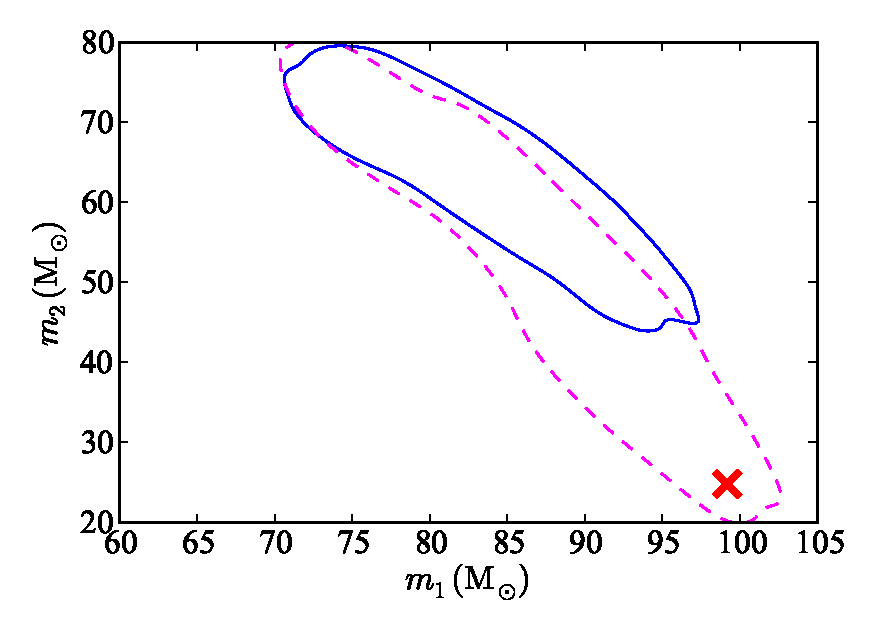
\includegraphics[width=0.45\textwidth]
{papers/nsbh_effectualness/figure8B.pdf}
\caption{\label{fig:nonspinavFF}
Average fitting factor between a set of generic, precessing, NSBH signals and a
template bank of non-spinning waveforms as a function of the component masses
(left) and as a function of the mass ratio and the black hole dimensionless spin
magnitude (right). Both the signals and the template waveforms are modelled
using the TaylorT4 approximant. The distribution that the NSBH
signals are drawn from is described in section \ref{sec:nsbhpop}.
Results obtained
using the zero-detuned, high-power advanced LIGO sensitivity curve with a 15Hz
lower frequency cut off.
}
\end{minipage}
\end{figure*}

\begin{figure*}
    \centering
    \begin{minipage}[l]{2.0\columnwidth}
    \centering
\includegraphics[width=0.45\textwidth]
{papers/nsbh_effectualness/figure9A.pdf}
\includegraphics[width=0.45\textwidth]
{papers/nsbh_effectualness/figure9B.pdf}
\caption{\label{fig:nonspinavFFT2}
Average fitting factor between a set of generic, precessing, NSBH signals and a
template bank of non-spinning waveforms as a function of the mass ratio and the
black hole dimensionless spin
magnitude (right). Shown when both the
template waveforms and signals are modelled with TaylorT2 (left) and when the
template waveforms are modelled with TaylorT2 and the signals are modelled with
TaylorT4 (right). The results in these plots are almost identical to each other 
and to the right panel of Fig.~\ref{fig:nonspinavFF}.
The distribution that the NSBH
signals are drawn from is described in section \ref{sec:nsbhpop}.
Results obtained
using the zero-detuned, high-power advanced LIGO sensitivity curve with a 15Hz
lower frequency cut off.
}
\end{minipage}
\end{figure*}

In Fig.~\ref{fig:nonspinavFF}, we show the mean fitting factor as a function
of the intrinsic parameters of the system when both templates and signals
were modelled with the TaylorT4 approximant. For comparison, in
Fig.~\ref{fig:nonspinavFFT2} we show the mean fitting factor as a function of
the spin magnitude and mass ratio for the TaylorT2 vs TaylorT2 results and the
TaylorT2 vs TaylorT4 results. In both cases the results are similar to the
TaylorT4 vs TaylorT4 case, which indicates that the results are not suffering
from a significant bias due to the choice of waveform approximant. However, we
note that when using TaylorT2 as the signal model, the performance of the
non-spinning banks is worse for high spin, unequal mass systems than when
using TaylorT4 as the signal model.

\begin{figure*}
    \centering
    \begin{minipage}[l]{2.0\columnwidth}
    \centering
\includegraphics[width=0.45\textwidth]
{papers/nsbh_effectualness/figure10A.pdf}
\includegraphics[width=0.45\textwidth]
{papers/nsbh_effectualness/figure10B.pdf}
\caption{\label{fig:nonspineffFF}
The signal recovery fraction obtained for a set of generic, precessing, NSBH
signals and a template bank of non-spinning waveforms as a function of the mass
ratio and the black hole dimensionless spin. Shown when both the
template waveforms and the signals are modelled with TaylorT2 (left) and when
both the template waveforms and the signals are modelled with TaylorT4 (right).
The distribution of the signal recovery fraction over the mass space is very 
similar to the distribution of average fitting factors shown in 
Figs.~\ref{fig:nonspinavFF} and \ref{fig:nonspinavFFT2}.
The distribution that the NSBH
signals are drawn from is described in section \ref{sec:nsbhpop}.
Results obtained
using the zero-detuned, high-power advanced LIGO sensitivity curve with a 15Hz
lower frequency cut off.
}
\end{minipage}
\end{figure*}

In Fig.~\ref{fig:nonspineffFF} we show
the signal recovery fraction as a function of the \ac{BH} spin magnitude and
the mass ratio. The signal recovery fraction is defined in section 
\ref{sec:bank_testing}.
It is clear that using a non-spinning bank to search for \ac{NSBH} systems will
result in a considerable reduction
in the \ac{NSBH} detection rate. In addition, the ability to
detect systems with high spin, especially systems that also have unequal 
masses, is especially poor.  We note that these efficiencies would be
improved by using non-spinning templates outside of the chosen mass ranges, for
example \ac{BNS} or binary black-hole template waveforms, or even templates
with unphysical mass parameters \cite{Brown:2012qf,Baird:2012cu}.

\subsection{Performance of aligned-spin template banks when searching for 
generic NSBH signals}
\label{sec:aligned_spin}

With the template banks of aligned-spin systems described in section
\ref{sec:bank_construction}, we are able to recover aligned-spin systems
modelled with either the TaylorT2 or TaylorT4 approximant with fitting factors
greater than 0.97 in $>99\%$ of cases, as shown in section
\ref{sec:bank_validation}.
If we use these banks to search for precessing systems modelled with the same
approximants, any loss in signal power, beyond that lost due to the spacing of
the aligned-spin bank, is entirely due to precession.
We now assess the performance of these aligned-spin banks when searching for
generic, precessing \ac{NSBH} signals and identify regions of the
parameter space where precessional effects cause a significant loss in
detection rate.

\begin{figure*}
    \centering
    \begin{minipage}[l]{2.0\columnwidth}
    \centering
\includegraphics[width=0.45\textwidth]
{papers/nsbh_effectualness/figure11A.pdf}
\includegraphics[width=0.45\textwidth]
{papers/nsbh_effectualness/figure11B.pdf}
\includegraphics[width=0.45\textwidth]
{papers/nsbh_effectualness/figure11C.pdf}
\includegraphics[width=0.45\textwidth]
{papers/nsbh_effectualness/figure11D.pdf}
\caption{\label{fig:aspinavFF}
Average fitting factor between a set of generic, precessing, NSBH
signals and a template bank of aligned-spin waveforms as a function of the
component masses (top left) and as a function of the
mass ratio and the black hole dimensionless spin
magnitude (top right). Also plotted is the minimum fitting factor (bottom left) 
and the signal recovery fraction (bottom right) as a function of the
mass ratio and the black hole dimensionless spin magnitude. Both signals and
template waveforms are modelled using the TaylorT4 approximant.
The distribution that the NSBH signals are drawn from
is described in section \ref{sec:nsbhpop}. The template bank construction
is described in section \ref{sec:bank_construction}. Results obtained
using the zero-detuned, high-power advanced LIGO sensitivity curve with a 15Hz
lower frequency cut off.
}
\end{minipage}
\end{figure*}

\begin{figure}
\includegraphics[width=0.45\textwidth]
{papers/nsbh_effectualness/figure12.pdf}
\caption{\label{fig:arseofsauron}
The distribution of precessing NSBH signals that are recovered with fitting
factors $< 0.7$ when searching with an aligned-spin template bank. We use
$\hat{J}$ to denote the initial total angular momentum of the system, $\hat{n}$
denotes the line of sight towards the observer
and $\hat{L}$ denotes the orbital angular momentum when the gravitational wave frequency is 60 Hz 
(at which point approximately half of the signal power has accumulated). 
Both signals and template waveforms are modelled using the TaylorT4 approximant.
The distribution that the NSBH signals are drawn from
is described in section \ref{sec:nsbhpop}. The template bank construction
is described in section \ref{sec:bank_construction}. Results obtained
using the zero-detuned, high-power advanced LIGO sensitivity curve with a 15Hz
lower frequency cut off.
}
\end{figure}

\begin{figure}
\includegraphics[width=0.45\textwidth]
{papers/nsbh_effectualness/figure13.pdf}
\caption{\label{fig:nsspin}
Average fitting factor between a set of generic, precessing, NSBH
signals and a template bank of aligned-spin waveforms as a function of the
mass ratio and the neutron star dimensionless spin
magnitude (top right). Both signals and
template waveforms are modelled using the TaylorT4 approximant.
The distribution that the NSBH signals are drawn from
is described in section \ref{sec:nsbhpop}. The template bank construction
is described in section \ref{sec:bank_construction}. Results obtained
using the zero-detuned, high-power advanced LIGO sensitivity curve with a 15Hz
lower frequency cut off.
}
\end{figure}


\begin{figure*}
    \centering 
    \begin{minipage}[l]{2.0\columnwidth}
    \centering
\includegraphics[width=0.45\textwidth]
{papers/nsbh_effectualness/figure14A.pdf}
\includegraphics[width=0.45\textwidth]
{papers/nsbh_effectualness/figure14B.pdf}
\caption{\label{fig:aspinavFFT2}
Average fitting factor between a set of generic, precessing, NSBH
signals and a template bank of aligned-spin waveforms as a function of the
mass ratio and the black hole dimensionless spin magnitude. Shown when both the
template waveforms and signals are modelled with TaylorT2 (left) and when the
template waveforms are modelled with TaylorT2 and the signals are modelled with
TaylorT4 (right). The results in these plots are almost identical to each other 
and to the top right panel of Fig.~\ref{fig:aspinavFF}.
The distribution that the NSBH
signals are drawn from is described in section \ref{sec:nsbhpop}. The
template bank construction is described in section \ref{sec:bank_construction}.
Results obtained
using the zero-detuned, high-power advanced LIGO sensitivity curve with a 15Hz
lower frequency cut off.
}
\end{minipage}
\end{figure*}

\begin{figure}
\includegraphics[width=0.45\textwidth]
{papers/nsbh_effectualness/figure15.pdf}
\caption{\label{fig:aspinimpr}
The fractional increase in the number of recovered signals when
searching for generic, precessing, NSBH signals using
a template bank of aligned-spin waveforms and a template bank of non-spinning
waveforms. Both signals and template waveforms are modelled using the TaylorT4
approximant. The distribution that the NSBH
signals are drawn from is described in section \ref{sec:nsbhpop}. The
template bank construction is described in section \ref{sec:bank_construction}.
Results obtained
using the zero-detuned, high-power advanced LIGO sensitivity curve with a 15Hz
lower frequency cut off.
}
\end{figure}

Our signal population is a set of 100,000 precessing \ac{NSBH} signals. This 
distribution was
described in section \ref{sec:nsbhpop}. For comparison this is the
\emph{same} set of signals as we used in section \ref{sec:non_spinning}.
As before, we will assess fitting factors using both the TaylorT2 and TaylorT4
models to mitigate any bias arising from choice of waveform model.
When TaylorT2 is used as the signal model, we will use the bank of aligned-spin
systems that was placed using the TaylorF2 metric and a 1000Hz
upper frequency cutoff and model the templates using the TaylorT2 approximant.
When TaylorT4 is used as the signal model, we will use the bank of aligned-spin
systems placed using the TaylorR2F4 metric and model the templates with
TaylorT4. The placement of these banks was described in section
\ref{sec:bank_construction}.

The results of these simulations can be seen in 
Fig.~\ref{fig:aspineffectualness}, where we also compare with the
results obtained in section \ref{sec:non_spinning} when using non-spinning
template banks. We can clearly see from Fig.~\ref{fig:aspineffectualness} that
the distribution of fitting factors for the
case when both signals and templates were modelled with TaylorT2 agrees well
with the case when both were modelled with TaylorT4. This indicates that
we have disentangled precessional effects from waveform-dependent effects and
our results are free of any bias due to the choice of waveform model.
The mismatches seen here, beyond that caused by the discreteness of the bank,
are due only to the effects of precession.
In both cases we observe a median fitting factor of
$\sim 0.95$ and a mean fitting factor of $\sim 0.91$. This is a clear
improvement
over the non-spinning results where the mean fitting factor was 0.82 (0.84) for
TaylorT2 (TaylorT4) and the median
fitting factor was 0.86 (0.88). 

In Fig.~\ref{fig:aspineffectualness} we also show results where the template
waveforms are modelled with TaylorT2 and the signals are modelled with TaylorT4.
In this case the performance is worse, with a median fitting factor of $\sim
0.92$ and a mean fitting factor of $\sim 0.88$.

In Fig.~\ref{fig:aspinavFF} we show the mean fitting factor as a function of
the intrinsic parameters
for our results with the TaylorT4 waveform. We also show the minimum fitting
factor and the signal recovery
fraction as a function of the \ac{BH} spin magnitude
and mass ratio for the same results.
The Figure serves to highlight that there are certain
systems in certain regions of the parameter space where precessional effects
cause the \ac{NSBH} signals to have large mismatches with a bank of
aligned-spin templates. This is most prominent when $m_{BH} / m_{NS}$ and the
\ac{BH} spin magnitude are both large, ie. where the black 
hole's angular momentum is particularly large relative to the orbital angular 
momentum. 
We explore this further in Fig.~\ref{fig:arseofsauron} where, following the
work of \cite{Brown:2012gs}, we show the distribution
of precessing systems recovered with fitting-factors smaller than $0.7$. This
is plotted as a function of the angles between the total angular 
momentum, the orbital angular momentum and the line of sight to an observer. 
As predicted in \cite{Brown:2012gs}, there is clearly a correlation
between these angles and the systems recovered with the lowest fitting factors.
To demonstrate that these results are not specific to the TaylorT4 waveform, in
Fig.~\ref{fig:aspinavFFT2} we show the mean fitting factor as a function of
the \ac{BH} spin magnitude and mass ratio for our TaylorT2 vs TaylorT2 and
TaylorT2 vs TaylorT4 results. The TaylorT2 results are very similar to the
TaylorT4 results in Fig.~\ref{fig:aspinavFF}. This again demonstrates that the
choice of waveform is not affecting our statements regarding the effect
precession will have on searches for \ac{NSBH} signals using aligned-spin
template banks. When searching for TaylorT4 signals with TaylorT2 templates
we see lower fitting factors. The disagreement between these two waveform models
is a significant factor that will affect searches for \ac{NSBH} systems with
second generation observatories. Computing higher order terms in the \acf{PN}
expansion of the center-of-mass energy and gravitational wave flux will help to
reduce this disagreement and produce waveforms that better match real
gravitational-wave signals. In Figure \ref{fig:nsspin} we plot the average 
fitting factor as a function of the mass ratio and the \emph{neutron star} 
dimensionless spin. There is not any noticeable correlation between the average 
fitting factor and the neutron star's spin.

We can also compare these results to the results we obtained using a
non-spinning template bank in section \ref{sec:non_spinning}. In 
Fig.~\ref{fig:aspinimpr} we show the fractional increase in the number
of recovered signals between using non-spinning and aligned-spin template banks
for the TaylorT4 approximant. The fractional increase in the number
of recovered signals is calculated by taking the ratio of the signal recovery 
fraction when using a non-spinning bank and the signal recovery fraction when 
using an aligned-spin bank. This figure helps to
emphasize that a much greater fraction of systems with large spin would be
recovered when using an aligned-spin template bank. In Table 
\ref{tab:results_summary} we summarize the average signal
recovery fractions for the aligned-spin banks and
compare these numbers to the results obtained with non-spinning template banks. 
We remind the reader that we are comparing signal recovery at a 
fixed signal-to-noise ratio. Signal recovery at a fixed false-alarm 
probability will depend on other factors, including the size of the parameter 
space covered by the template bank and the non-Gaussianity of the data. We 
discuss this further in the conclusion.

\begin{table*}
    \centering
    \begin{minipage}[l]{2.0\columnwidth}
    \centering
\begin{tabular}{p{1.6cm}|p{1.6cm}|p{1.85cm}|p{1.85cm}|p{1.85cm}|p{1.85cm}|p{
1.85cm}|p{1.85cm}}
\,\,\,\,\,\,Template  & \,\,\,\,\,\, Signal  & 
\multicolumn{2}{|p{3.7cm}|}{Signal recovery fraction
for non-spinning bank} & \multicolumn{2}{|p{3.7cm}|}
{Signal recovery fraction for aligned-spin bank} & 
\multicolumn{2}{|p{3.7cm}} {Fractional improvement
in signal recovery} \\ \cline{3-8}
 approximant & approximant & Average & $(10,1.4)M_{\odot}$ & Average
& $(10,1.4)M_{\odot}$ & Average & $(10,1.4)M_{\odot}$\\
\hline \hline
 TaylorT2 & TaylorT2 & 64\% & 63\% & 83\% & 74\% & 30\% & 17\% \\
 TaylorT4 & TaylorT4 & 69\% & 67\% & 82\% & 73\% & 19\% & 9\% \\
 TaylorT2 & TaylorT4 & 67\% & 64\% & 77\% & 67\% & 16\% & 5\% \\
\end{tabular}
\caption{\label{tab:results_summary}
The performance of our aligned-spin template banks when used to search for a
set of generic, precessing, NSBH signals using varying approximants for the
template and signal waveforms. We show both the mean signal recovery fraction 
over the full \ac{NSBH} signal population we consider and the signal recovery 
fraction for a \ac{NSBH} system with masses $(10\pm0.5,1.4\pm0.05)M_{\odot}$.
The distribution that
the NSBH signals are drawn from is described in section \ref{sec:nsbhpop}. The
template bank construction is described in section \ref{sec:bank_construction}.
Results obtained
using the zero-detuned, high-power advanced LIGO sensitivity curve with a 15Hz
lower frequency cut off and a 1000Hz upper frequency cut off.
}
\end{minipage}
\end{table*}

Finally, we compare our results with previous works. In \cite{Ajith:2012mn}
the authors presented an efficiency study when using a template bank of 
stochastically generated aligned-spin signals. We verified that when using the 
stochastic algorithm we used in this work, and using the same set of parameters 
as the study described in \cite{Ajith:2012mn}, we generated a bank with the 
same number of templates. We have therefore demonstrated that our template bank 
algorithm requires less templates to acheive the same level of coverage as the 
algorithm used in \cite{Ajith:2012mn}. In that work the effective fitting 
factor for a \ac{NSBH} system with masses given by $10 M_{\odot}$ ,
$1.4 M_{\odot}$ was estimated to be 0.95, which corresponds to a
signal recovery fraction of 86\%.
In contrast, our results show a lower signal recovery fraction 
for the same masses of $73 - 74\%$ when the same waveform model is used to 
model both the template and signal. It isn't clear why this discrepancy 
occurs, however it may be partially explained by the fact that 
the authors of \cite{Ajith:2012mn} used a lower frequency cutoff in their 
matched-filters of 20Hz, whereas we used 15Hz, which is more appropriate for the 
predicted \ac{aLIGO} zero-detuned--high-power noise curve. 

In \cite{Brown:2012gs} the authors used a simplified model of precessing systems
to predict the distribution of fitting
factors for \ac{NSBH} systems. These results, shown in Figure 11 of that work,
agree qualitatively with the results obtained here.
We also obtain quantitative agreement by comparing our simulations of 
generic precessing systems with TaylorT4 as the signal and template model with 
the values predicted by Eq. 46b of \cite{Brown:2012gs}. We find that 90\% of 
the fitting factors are within $0.03$ of the predicted values.
They also predicted the 
distribution of the signals that would be recovered with the lowest fitting 
factors as a function of the orientation of the black hole spin and the 
orientation of the orbital plane with respect to the line of sight. We produce 
a similar distribution in Fig.~\ref{fig:arseofsauron}. 
A further exploration of the agreement of the fitting factors with 
this prediction will be carried out in a future work making use of these 
simulations.

\section{Conclusions}
\label{sec:conclusion}

In this work we have explored the effect that the angular momentum of the black
hole will have on searches for neutron-star black-hole binaries with
\ac{aLIGO}. The black hole's angular momentum will affect the phase evolution
of the emitted gravitational-wave signal, and, if the angular momentum is
misaligned with the orbital plane, will cause the system to precess. We have
found that if these effects are neglected in the filter waveforms used to
search for \ac{NSBH} binaries it will result in a loss in detection rate of
$31-36\%$ when searching for \ac{NSBH} systems with masses uniformly 
distributed in the range 
$(3-15,1-3)M_{\odot}$. When restricting the masses to 
$(9.5-10.5,1.35-1.45)M_{\odot}$ we find that the loss in detection rate is
$33 - 37\%$. The error in these measurements is due to uncertainty in 
the \ac{PN} waveform models used to simulate \ac{NSBH} gravitational-wave 
signals.  In a companion work we investigate how the uncertainty in waveform 
models used to simulate \ac{NSBH} waveforms will reduce detection 
efficiency~\cite{Nitz:2013mxa}. 

We have presented a new method to create a template bank of \ac{NSBH} filter
waveforms, where the black hole's angular momentum is
included, but is restricted to be (anti-)aligned with the orbit. These
waveforms will include the effect that the black hole's angular momentum has on
the phase evolution of the gravitational-wave signal, but will not include any
precessional effects. We have shown that this bank offers a
$16\%-30\%$ improvement in the detection rate of neutron-star black-hole
mergers when compared to a non-spinning template bank when searching for 
\ac{NSBH} systems with masses in the range $(3-15,1-3)M_{\odot}$. However, when
searching for \ac{NSBH} systems with masses restricted to the range 
$(9.5-10.5,1.35-1.45)M_{\odot}$ we find the improvement is reduced to $5-17\%$.
Some systems are not recovered well with this new bank of filters. These systems
are ones where the black-hole spin is misaligned with the orbit and the waveform
is significantly modified due to precession of the orbital plane. This happens
most often when $m_{BH} / m_{NS}$ and the spin magnitude are both large. In
\cite{Brown:2012gs} the authors predict where in the parameter space to expect
\ac{NSBH} systems that will not be recovered well by non-precessing template
banks. These predictions were
given in terms of the angles between the orbital plane, the black hole's angular
momentum and the line-of-sight to an observer. These predictions agree with the
results that we obtain in this work. In \cite{Ajith:2012mn} the authors claim
that an aligned-spin template bank will be effectual for detecting precessing
\ac{NSBH} systems. In this work, we find that with an aligned-spin template
bank $17-23\%$ of \ac{NSBH} systems will be missed compared to an ideal search
with
exactly matching filter waveforms. In reality this ideal search could never
be performed as it would require an infinite number of filter waveforms.
Template banks are usually constructed to allow for no more than a 3\% loss in
\ac{SNR}, therefore we expect to lose up to $10\%$ of systems even if the
template bank fully covers the signal parameter space. We therefore conclude
that searches using precessing waveforms as templates could potentially
increase the detection rate of \ac{NSBH} signals, but not by more than $\sim
20\%$. Performing such a search would, however, remove an observational bias
against systems where precessional effects are most prevalent in the
gravitational-wave signal.

These figures are also affected by the 
parameter distribution chosen for the \ac{NSBH} systems. Here we chose a 
distribution that is uniform in mass, uniform in spin magnitudes, isotropic in 
spin orientations and isotropic in orientation parameters and sky location. We 
have however, explored how the ability to detect precessig \ac{NSBH} signals 
varies as a function of the masses and spins as seen in Figures 
\ref{fig:aspinavFF} and \ref{fig:arseofsauron}. 

When searching for \ac{NSBH} systems in \ac{aLIGO} one has to
consider the non-Gaussianity of the background noise, which we have not done in
this work. A non-Gaussian noise
artifact can produce \acp{SNR} that are considerably larger than those expected
from Gaussian noise fluctutations. To deal with this, numerous
consistency tests are used in the analyses to separate gravitational wave
signals from instrumental noise artifacts \cite{Babak:2012zx}. It is possible
that the detection rate could be further reduced from the values we quote in
this work if some signals \emph{fail} these consistency tests and are
mis-classified as non-Gaussian noise transients.
However, these signal consistency tests should only act to remove, or reduce the
significance of, events that already have low fitting factors and therefore do
not match well with the search templates. 
Another important consideration is that of the
number of templates used in the bank. To achieve higher fitting factors will
require more template waveforms, covering a larger signal space, which will 
allow more freedom in matching the
background noise and will mean that the \ac{SNR} of the loudest background
triggers will increase. Therefore signals will need slightly higher \acp{SNR} to
achieve the same false alarm probability. However, a factor of 10 increase in
the number of \emph{independent} templates will only increase the expected
\ac{SNR} of the loudest background event by less than $5\%$, if 
Gaussian noise is assumed. Therefore, while we
are careful to note these considerations, we do not believe they will have a
large impact on the numbers we quote above and leave a detailed investigation of
such effects to future work.

In this work we have restricted ourselves to 
considering post-Newtonian, inspiral-only signal waveforms and consider only the 
case of two point particles. This was done as there is not currently any widely 
available waveform model that includes both the full evolution of a \ac{NSBH} 
coalescence \emph{and} includes precessional effects over the full parameter 
space that we consider. When such a model is available it may be that 
tidal forces and the merger component of the waveform may affect our 
conclusions. We believe that such effects will be limited as the
black hole mass is $< 15 M_{\odot}$ in our simulations, however it would be 
informative to repeat our simulations when a full \ac{NSBH} waveform model is 
available.



\Chapter{Improvements to the CBC Search Pipeline}
\label{ch:single_stage}
\documentclass[12pt]{iopart} \usepackage{graphicx,amssymb}
\expandafter\let\csname equation*\endcsname\relax
\expandafter\let\csname endequation*\endcsname\relax
\usepackage{amsmath}
%\usepackage[font={small,it}]{caption}
\usepackage[usenames,dvipsnames]{xcolor}
% This is for strikeout font
\usepackage[normalem]{ulem}
\usepackage{multirow}
\normalem
\usepackage{lscape}
\usepackage{cite}
\usepackage[symbol*]{footmisc}
\usepackage{url}
\usepackage{hyperref}

\newcommand{\newcomment}[1]{\textcolor{red}{[#1]}}
\newcommand{\iancomment}[1]{\textcolor{magenta}{[#1]}}
\newcommand{\duncancomment}[1]{\textcolor{red}{[#1]}}
\newcommand{\samcomment}[1]{\textcolor{violet}{[#1]}}
\newcommand{\marcelcomment}[1]{\textcolor{green}{[#1]}}
\newcommand{\stevecomment}[1]{\textcolor{blue}{[#1]}}
\newcommand{\harald}[1]{\textcolor{olive}{[#1]}}

\newcommand{\splitcell}[2][c]{%
  \begin{tabular}[#1]{@{}c@{}}#2\end{tabular}}

\pdfminorversion=4
\hyphenation{Schwarz-schild wave-form wave-forms}
\sloppypar


%=============================================================================

\begin{document}

\title[An improved pipeline for CBC GW searches]{An improved pipeline to search for gravitational waves from compact
binary coalescence}

\author{Samantha A. Usman$^1$,
        Marcel S. Kehl$^{2,3}$,
        Alexander H. Nitz$^1$, \\
        Ian W. Harry$^{1,4}$,
        Duncan A. Brown$^1$,
        Collin D. Capano$^{5,6}$,
        Thomas Dent$^6$,
        Stephen Fairhurst$^7$, 
        Harald P. Pfeiffer$^{2,8}$, \\
        Christopher M. Biwer$^1$, 
        Tito Dal Canton$^6$,
        Drew Keppel$^6$, \\
        Peter R. Saulson$^1$,
        Matthew West$^1$, 
        Joshua L. Willis$^{6,9}$.}

\address{$^{1}$ Department of Physics,
         Syracuse University, Syracuse, NY 13244, USA}

\address{$^{2}$ Canadian Institute for Theoretical Astrophysics,
         University~of~Toronto, Toronto, Ontario M5S 3H8, Canada}

\address{$^3$ Max-Planck-Institut f{\"u}r Radioastronomie, Auf dem H{\"u}gel 69,  53121 Bonn, Germany}

\address{$^4$ Max-Planck-Institut f{\"u}r Gravitationsphysik,
         Albert-Einstein-Institut, Am M\"uhlenberg 1,
         D-14476 Golm, Germany}

\address{$^5$ Maryland Center for Fundamental
         Physics \& Joint Space-Science Institute,
         Department of Physics,
         University of Maryland, College Park, MD 20742, USA}

\address{$^6$ Max-Planck-Institut f{\"u}r Gravitationsphysik,
         Albert-Einstein-Institut, D-30167 Hannover, Germany}

\address{$^7$ Cardiff University, Cardiff CF24 3AA, United Kingdom}

\address{$^8$ Canadian Institute for Advanced
  Research, 180 Dundas St.~West, Toronto, ON M5G 1Z8, Canada}

\address{$^9$ Abilene Christian University, Abilene, TX 79601, USA}

\ead{samantha.usman@ligo.org}

\vspace*{-0.1cm}
\begin{abstract}
The second generation of ground-based gravitational-wave 
detectors will begin taking data in September 2015. Sensitive and
computationally-efficient data analysis methods will be required to maximize
what we learn from their observations. In this paper, we describe improvements
made to the offline analysis pipeline searching for gravitational waves from
stellar-mass compact binary coalescences, and assess how these improvements
affect search sensitivity. Starting with the two-stage \texttt{ihope} pipeline
used in S5, S6 and VSR1-3 and using two weeks of S6/VSR3 data as test periods,
we first demonstrate a pipeline with a simpler workflow. This
\emph{single-stage pipeline} performs matched filtering and coincidence
testing only once. This simplification allows us to reach much lower
false-alarm rates for loud candidate events. We then describe an optimized
$\chi^2$ test which minimizes computational cost. Next, we compare methods of
generating template banks, demonstrating that a fixed bank may be used for
extended stretches of time. Fixing the bank reduces the cost and complexity,
compared to the previous method of regenerating a template bank every 2048 s
of analyzed data. Creating a fixed bank shared by all detectors also allows us
to apply a more stringent coincidence test, whose performance we quantify.
With these improvements, we find a 10\% increase in sensitive volume
with a negligible change in computational cost. 
\end{abstract}

\vspace*{-0.4cm}
\pacs{04.30.-w,04.25.-g}
% 04.25.dg      Black holes -> black-hole binaries
% 04.30.-w      Gravitational waves -> general relativity
% 04.25.D-      Relativity -> general relativity
%                          -> numerical relativity
% 04.25.-g      Relativity -> general relativity
%                          -> approximation methods, equations of motion


%=============================================================================

\section{Introduction}
\label{s:intro}

Coalescing binaries containing compact objects~\cite{Cutler:1992tc} are likely
candidates for detection by the ground-based gravitational-wave observatories
LIGO \cite{Abbott:2007kv}, VIRGO \cite{Accadia:2012zzb}, and KAGRA
\cite{Akutsu:2015hua}. Searches for gravitational waves from compact object
binaries containing neutron stars and stellar-mass black holes have been
performed using the first-generation LIGO and Virgo detectors in LIGO's six
science runs (S1--S6) and three Virgo science runs
(VSR1--VSR3)~\cite{Abbott:2003pj,Abbott:2005pe,Abbott:2005kq,Abbott:2007xi,Abbott:2007ai,Abbott:2009tt,Abbott:2009qj,Abadie:2010yba,Abadie:2011nz}.
Construction of the Advanced LIGO (aLIGO) detectors~\cite{TheLIGOScientific:2014jea} is now complete and the
first aLIGO observing runs are scheduled for autumn 2015~\cite{Aasi:2013wya}.
The Advanced Virgo (AdV) detector~\cite{Acernese:2015gua} is scheduled to join this network in 2016.
When these second-generation detectors reach design sensitivity, it is
predicted that they will observe on the order of $10$ coalescence events per
year~\cite{Abadie:2010cf}. Binaries containing neutron stars and stellar-mass
black holes are likely to be the first sources observed by aLIGO and AdV. 

Gravitational waves from compact binary coalescence have three distinct
phases: an \emph{inspiral} consisting of a wave of slowly increasing amplitude
and frequency, a \emph{merger} which can be calculated using numerical
simulations, and a \emph{post-merger} signal as the binary stabilizes into a final
state. If the total mass of the binary is lower than $M \lesssim 12\,
M_\odot$~\cite{Buonanno:2009zt,Brown:2012nn}
and the angular momenta of the compact objects (their \emph{spin}) is
small~\cite{Nitz:2013mxa,Kumar:2015tha}
(as is the case for binary neutron stars), then the inspiral phase can be 
well modeled using the post-Newtonian approximations (see e.g.
Ref.~\cite{Blanchet:2013haa} for a review).  For higher mass and higher-spin
binaries, analytic models tuned to numerical relativity can provide accurate
predictions for the gravitational waves from compact 
binaries~\cite{Buonanno:1998gg,Pan:2009wj,Damour:2012ky,Taracchini:2013rva,Damour:2014sva}. 

Ground-based gravitational-wave detectors produce a calibrated strain signal
$s(t)$, which is sensitive to gravitational waves incident on the detector's
arms~\cite{Abadie:2010px}. In addition to possible signals, the strain data contain two classes of
noise: (i) a primarily stationary, Gaussian noise component from fundamental
processes such as thermal noise, quantum noise, and seismic noise coupling
into the detector; and (ii) non-Gaussian noise transients of instrumental and
environmental origin. Since the gravitational-wave signal from compact
binaries is well-modeled and the expected amplitude of astrophysical signals is
comparable to the amplitude of the noise,
matched filtering is used to search for signals in the detector data~\cite{Allen:2005fk}.  Since
we do not \emph{a priori} know the parameters of the compact
binaries we may detect, a \emph{bank} of template waveforms is constructed that spans the astrophysical
signal space~\cite{Sathyaprakash:1991mt,Dhurandhar:1992mw,Owen:1995tm,Owen:1998dk,Babak:2006ty,Cokelaer:2007kx,Brown:2012qf,Keppel:2013yia,Keppel:2013uma}. These banks are designed so that the loss in event rate caused by
their discrete nature is typically no more than 10\%. The exact placement of the
templates depends on the noise power spectral density of the detector data. To
mitigate the effect of the non-Gaussian noise transients in the search, we
require that any signal be seen with consistent parameters (compact objects'
spins and masses and the signal's time of arrival) in the detector network. Additional
statistical tests are applied to mitigate the effect of non-Gaussian
noise transients~\cite{Allen:2004gu}; these are often called \emph{signal-based vetoes}. The 
matched-filter signal-to-noise ratio and the additional statistical tests are used to
create a numerical detection statistic for candidate signals. To assign a
statistical significance to these detection candidates, the network's false-alarm rate is computed as a function of the detection statistic for the
noise background.  To determine the performance of the search, simulated
signals are added to the detector data and we record the search's ability to
identify and measure the significance of these simulated gravitational waves.

Executing the steps described above is the task of the \emph{search pipeline.}
While the basic steps remain the same, different choices can be made to
create various configurations and topologies for a search pipeline. The search
pipelines used in the last joint LIGO-Virgo science run (S6/VSR2,3) used the
\texttt{ihope} search pipeline to search for compact
binaries~\cite{Babak:2012zx}. The \texttt{ihope} pipeline, as well as the
pipelines used in previous LIGO-Virgo
searches~\cite{Brown:2004pv,Brown:2005zs}, are \emph{offline} search
pipelines. These pipelines analyze the data in a batch mode, processing
of the order of one week of data from the network. Offline batch
processing allows the pipeline to incorporate additional information about the
quality of the detector data or search tuning that is not available in real
time~\cite{Aasi:2012wd,Aasi:2014mqd}, and to produces a systematic false-alarm rate
estimation of candidates by using large samples of the noise background before
and after the time of a signal. Batch processing also allows the pipeline to
take advantage of the computationally efficient Fast Fourier Transform (FFT)
when implementing matched filtering~\cite{Allen:2005fk}, and allows
computational tasks to be parallelized over time and binary parameters for
efficient implementation on large computing clusters~\cite{Brown:workflow}.

In this paper, we focus on the offline search pipeline that will be used to 
search for compact binary coalescence signals in aLIGO and AdV.  We describe 
several proposed modifications
to the \texttt{ihope} search pipeline to create a simpler, more sensitive
search pipeline and to reduce the computational cost of the search. These
improvements include: (i) changing the pipeline workflow from the
\emph{two-stage} analysis described in Ref.~\cite{Babak:2012zx}, where two
coincidence tests are applied to reduce the computational cost of signal-based
vetoes, to a \emph{single-stage} pipeline with one coincidence test; (ii) a 
more efficient algorithm for computing the signal-based veto
used in previous LIGO-Virgo searches; (iii) improved methods for using
time-shifted detector data to estimate the significance of candidates; (iv) use
of third-and-half order post-Newtonian waveforms to place the bank of templates
used for matched filtering~\cite{Keppel:2013kia}; (v) simplifying template 
placement by using a power
spectral density estimate over longer periods of time, and by using a shared
template bank in all detectors~\cite{Keppel:2013uma}; (vi) improvements to the methods use to
determine if candidate events are coincident in the detector network. 

In this analysis, we have configured the pipeline to search for non-spinning
compact object binaries with a total mass between 2 and 25\ M$_{\odot}$ using
3.5 post-Newtonian order TaylorF2 waveforms in the matched filter. The
TaylorF2 waveform is constructed using the stationary phase approximation and
includes only the inspiral portion of the waveform~\cite{Droz:1999qx}.  We use
data from LIGO's sixth science run to test the search pipelines. These data
are dominated by seismic noise frequencies below 40~Hz. We therefore set the
starting frequency for these template waveforms at 40~Hz, with the templates
terminating at the frequency of the innermost stable circular orbit for a test
particle in the spacetime (ISCO). These parameters are chosen to be the same
as for the S6/VSR2,3 search described in Ref.~\cite{Abadie:2011nz}. However,
since that analysis it has been shown that searches for signals with total
mass above $\sim 12\ M_\odot$ should use templates that capture the full
inspiral-merger-ringdown signal to obtain the maximum signal-to-noise
ratio~\cite{Brown:2012nn}. Furthermore, since the simulated signals that are used to test search
sensitivity are generated in the time domain, they are generated using a different
post-Newtonian approximant than the frequency-domain filter templates. The
maximal mass of the injected systems is therefore restricted by the
uncertainties of the post-Newtonian waveforms. For total masses below $\sim
14\ M_\odot$, it has been shown that the discrepancy between post-Newtonian
models is negligible~\cite{Buonanno:2009zt}. Consequently, we set the upper
limit of the injections to $\sim 14\ M_\odot$. We discard templates
corresponding to chirp masses higher than $6.1 \ M_\odot$ in post-processing.
This is equivalent to ignoring the results of the highest mass bin in the
S6/VSR2,3 search, allowing us to make a direct comparison to the S6/VSR2,3
results in a region where post-Newtonian waveforms are known to be valid for
aLIGO and AdV.  We determine the effect of the proposed changes to the search
pipeline by comparing the sensitivity of the search in two weeks of LIGO data
from the sixth LIGO science run to its performance on two weeks of stationary,
Gaussian noise. We also perform large-scale injections of simulated signals to
measure the sensitivity of the search pipeline as a function of false-alarm
rate. Searches for higher mass systems and searches using template waveforms
that incorporate spin have been also been
performed~\cite{Abbott:2007ai,Abadie:2011kd,Aasi:2012rja,Privitera:2013xza,Canton:2014ena},
but they are outside the scope of this work. 

We show that the new pipeline is substantially simpler than that of
Ref.~\cite{Babak:2012zx} and that it can calculate false-alarm rates to $\sim
1/10,000$ years on one week of LIGO data. The performance of the search
pipeline in LIGO S6 data is very close to that of stationary, Gaussian noise.
The computational cost of the improved pipeline is also comparable to the
pipeline used in previous science runs. We show that together, our proposed
improvements yield approximately a 10\% improvement in search sensitive volume
at a false-alarm rate of $1/1000$ years. Given these advantages, we propose
that this pipeline be used as the basis for offline searches for compact
binary coalescence in future LIGO and Virgo observing runs.  We note some additional improvements
that can be made to the pipeline before aLIGO and AdV's first observing runs.

The rest of this paper is organized as follows: in Sec.~\ref{s:search}, we
describe the methods used to search for coincident
detector searches for compact binary coalescence. In Sec.~\ref{s:methods} we
review the \texttt{ihope} pipeline used in S6/VSR2,3, describe the
improvements that we propose, and our methods for testing these improvements.
For aLIGO and AdV the pipeline workflow generator, template placement, and
filtering engine have been substantially re-written as part of the PyCBC
package~\cite{Canton:2014ena}. Our changes beyond the \texttt{ihope}
pipeline are implemented in PyCBC for use in upcoming LIGO and Virgo observing
runs.  Sec.~\ref{s:results} describes how each of our proposed changes affects
the sensitivity of the search pipeline.  Finally, Sec.~\ref{s:conc} shows the
overall improvement from each of these changes and we suggest directions for
further possible improvements to the search pipeline.

\section{Coincident Matched-Filter Search for Compact Binaries}
\label{s:search}

To search for coalescing compact binaries with LIGO and Virgo, the offline search
pipeline implements a coincident matched-filter search.  If the detector noise
was stationary and Gaussian, matched filtering alone would be sufficient to
determine the statistical significance of a signal. For such stationary noise, 
demanding that the signal is present in two or more detectors in the network 
(coincidence) would provide a sufficiently low false-alarm rate to claim a 
detection at a matched-filter network signal-to-noise ratio of 8; the signal 
strength used to estimate aLIGO's event rate in Ref.~\cite{Abadie:2010cf}.
However, the presence of non-stationary and non-Gaussian noise
transients (\emph{glitches})
in the detector noise increases the false-alarm rate at a given
signal-to-noise ratio and additional statistical tests must be used to separate
signals from noise. The output of the matched filter is combined with these
additional tests to create a new detection statistic for coincident detection
candidates. To determine the significance of these candidates, the noise
background must be estimated to create a map between the numeric value of the
detection statistic and the false-alarm rate (or, equivalently, false-alarm
probability). Background noise is estimated by performing coincidence tests on
detector data which has been time-shifted such that coincident candidates no
longer represents a coincident detection. The search pipeline consists of
several stages which are applied to the data to construct coincident detection
candidates and measure their significance.   Below, we describe the different
stages used in offline compact object binary search pipelines. We then review
the \texttt{ihope} search pipeline used in the S6/VSR2,3 LIGO-Virgo search for
low-mass compact binaries and describe our proposed improvements.  For each
proposed improvement, we use the methods described in Sec.~\ref{s:methods} to
assess the impact on the search sensitivity. The results of these tests are
presented in Sec.~\ref{s:results}.

To search for gravitational waves from compact binaries, the search pipeline
first locates the data from the detectors, which is stored on disk. Analysis
of the week of data can be parallelized over time and over detector allowing
the search to execute multiple search programs simultaneously that process
small blocks of data for each detector. In this analysis, the
analysis block size is set to $2048$ seconds, as in the S6/VSR2,3 search.
The data is first used to construct the
template bank that will be used to matched filter the
data~\cite{Sathyaprakash:1991mt,Dhurandhar:1992mw,Owen:1995tm,Owen:1998dk,Babak:2006ty}.
The bank is constructed by specifying the boundaries of the target
astrophysical space and the desired \emph{minimal match}, the fractional loss in
matched-filter signal-to-noise ratio caused by the discrete nature of the bank.
The minimal match is chosen so that the bank is dense enough that any
gravitational wave in the target space can be recovered with a loss of
signal-to-noise ratio no greater than a chosen maximum, usually set to 3\%~\cite{Abbott:2011ys}. 
A metric is constructed on the signal space that
locally measures the fractional loss in signal-to-noise ratio for varying mass
parameters of the templates~\cite{Owen:1998dk}.  This metric (and hence
the template placement) depends on the power spectral density of the
detector noise. Since inspiral signals have more cycles at lower frequencies,
a detector with better low-frequency sensitivity relative to high frequencies
will have more discriminating power and thus require a denser bank to maintain
the desired minimal match. Considering the noise properties of S6 data, we chose the
lower-frequency cutoff for bank generation and filtering to be $40$~Hz, and
the boundaries of the template bank are specified by $1\, M_\odot \le m_1,
m_2$ and $m_1 + m_2 \le 25 M_\odot$.

The pipeline then matched filters the template waveforms against the data.
 The matched filter consists of a weighted inner product in the frequency
domain used to construct the (squared) signal-to-noise ratio, given by
%
\begin{equation}
\rho^2(t) = \frac{(s|h_c)^2 + (s|h_s)^2}{(h_c|h_c)} \, ,
\label{eq:snr}
\end{equation}
%
where $h_c$ and $h_s$ are the two orthogonal phases of the 
%
\begin{equation}
(s|h)(t) = 4\int_{f_{low}}^{f_{high}} \frac{\tilde{s}(f)\tilde{h}^*(f)}{S_n (f)}e^{2\pi i f t}\, \mathrm{d}f.
\label{eq:ip}
\end{equation}
%
Here $\tilde{s}$ denotes the Fourier-transformed detector data and $\tilde{h}$
denotes the Fourier-transformed template waveform. As in the S6/VSR2,3 search,
each 2048 second block of data is sub-divided into fifteen $256$ second
segments, each overlapped by $128$ seconds. The noise power spectral
density $S_n(f)$ is computed by taking the bin-by-bin median of each of the power
spectral density of each of the fifteen segments. The fifteen segments are then each
matched filtered, with the first and last $64$ seconds of each segment
ignored, due to corruption of the filter by FFT
wrap-around~\cite{Allen:2005fk}

Times when the signal-to-noise ratio exceeds a pre-defined threshold are
considered gravitational-wave candidates, called
\emph{triggers}\cite{Allen:2005fk}. This threshold is set to a
signal-to-noise ratio of 5.5.  Since the signal-to-noise ratio can exceed
this threshold for many sample points around the time of a signal, clustering
is performed on these triggers in time, so that one trigger can be associated
with a signal. Here we use the template-length based clustering of 
Ref.~\cite{Allen:2005fk}, as in the S6/VSR2,3 search. 
For a sufficiently loud event, several nearby templates in the
bank may also produce triggers associated with the same signal and so
clustering over the template bank can also be used to limit the number of
triggers produced by the search. The S6/VSR2,3 search used a 30~ms time window
to cluster over the bank; we investigate this, as well as methods that use no
template bank clustering, as described in Sec.~\ref{s:coinc}.

Since non-Gaussian noise transients in the data can also produce excursions in
the signal-to-noise ratio, an additional signal-based veto is then constructed
to ensure that the matched filter signal-to-noise ratio is
consistent with an inspiral signal. To construct this test, the
template is split into $p$ bins of equal power, and a matched filter $\rho_l$
constructed for each of these bins. Triggers are then subject to the
$\chi^2$ test, given by
%
\begin{equation}
\chi^2 = p\displaystyle\sum_{l=1}^{p}\left[\left(\frac{\rho_c}{p}-\rho_c^l\right)^2 + \left(\frac{\rho_s}{p}-\rho_s^l\right)^2 \right] \, ,
\label{eq:chisqr}
\end{equation}
%
where $\rho_c$ and $\rho_s$ are the two orthogonal filter phases.
Real gravitational-wave signals would return a low number for the $\chi^2$
test, while candidates caused by noise transients will
return a high number for the $\chi^2$ test~\cite{Allen:2004gu}. As in the 
S6/VSR2,3 analysis, we set $p = 16$. The value of the $\chi^2$ test is used to 
calculate a new detection statistic, called the \emph{reweighted
signal-to-noise ratio}, given by 
%
\begin{equation}
\hat{\rho} =
  \begin{cases}
    \rho &\textrm{for } \chi^2 \leq n_\mathrm{dof}\\
    \rho[\frac{1}{2}(1+(\frac{\chi^2}{n_{dof}})^3)]^{-\frac{1}{6}} &\textrm{for } \chi^2 > n_\mathrm{dof} ,
  \end{cases}
\label{eq:newSNR}
\end{equation}
where $n_\mathrm{dof} = 2p-2$ is the number of degrees of freedom in the
$\chi^2$ test~\cite{Babak:2012zx}.
%
Since candidates caused by noise transients generally return a high $\chi^2$
statistic, the new detection statistic down weights the signal-to-noise ratio
of candidates by dividing with the $\chi^2$ statistic~\cite{Abadie:2011nz}.

The quality of the data generated by the LIGO and Virgo detectors is
scrutinized to mitigate noise and to improve the reach of the 
detectors~\cite{Aasi:2012wd,Aasi:2014mqd}. Data
quality investigations characterize times of poor detector performance
according to three broad classifications: (i) the data quality is sufficiently
poor that the data should be discarded; (ii) an instrumental artifact with a
known physical coupling to the recorded strain is observed by monitoring
environmental or auxillary control channels; (iii) a statistical correlation
is observed between a high trigger rate from the search and excess noise power
in environmental or auxillary control channels. The first class of data is
removed before searching for signals. For the second two classes, a \emph{data
quality veto} is created. Vetoes are time intervals during
which the pipeline removes all candidate events from the search.
Improved methods for tuning and applying vetoes in compact object binary
searches have been investigated~\cite{Canton:2013joa}, however these methods
were not used in S6/VSR2,3. Investigation of these new approaches is outside
the scope of this work and we apply the same data-quality vetoes as
they were tuned for the S6 search.

A true gravitational-wave signal would be incident on all detectors in the network at
approximately the same time. The maximum time-of-arrival difference between
detectors is given by the light-travel time between observatories. Noise,
however, will be independent between detectors since the interferometers
are far apart. For this reason, we require the candidates to be coincident
between detectors: they must arrive within the light-travel time between detectors,
approximately 11 milliseconds for the two LIGO detectors, with
a few milliseconds of padding to account for timing errors. The pipeline also
requires that the mass parameters of the signal are consistent between all
detectors, as would be expected for a true gravitational wave. 
It is possible to construct several different types of tests for
signal coincidence: early LIGO analyses used a simple, independent check on
the consistency of the time of arrival and mass. Ref.~\cite{Robinson:2008un}
introduced a new method, applied to later analyses, including searches using S5, 
S6, and Virgo data, that uses
the template bank metric to construct an ellipse of a given size around a
trigger. Overlap of these ellipses is then used to determine if triggers are coincident. In this
paper, we compare the ellipsoidal coincidence method, as used in the S6/VSR2,3 search,
with a new coincidence method that used the
ellipsoidal method for the time of the trigger, but demands that the two mass
parameters of the trigger match exactly.

To claim a detection of gravitational waves, it is necessary to calculate the
false-alarm rate of the candidate and demonstrate that it is very unlikely to
occur due to noise in the detectors. To measure the noise background in the
search, the pipeline shifts the triggers generated by filtering each
detector's strain data by an amount greater than the light-travel time between
detectors, and applies the coincidence test again.  Coincident triggers that
occur in the shifted data cannot be due to gravitational waves and thus represent
background noise. By repeating this test with many different time lags, we can
obtain a good estimate of the rate of background triggers as a function of the
combined reweighted signal-to-noise ratio detection statistic. For the 
two-detector network considered here, the combined statistic is given by
%
\begin{equation}
\hat{\rho}^c = \sqrt{\hat{\rho}_\mathrm{L1}^2 + \hat{\rho}_\mathrm{H1}^2},
\end{equation}
%
where H1 is the LIGO Hanford detector and L1 is the LIGO Livingston detector. 
The map between $\hat{\rho}^c$ and false-alarm rate allows us to estimate the
significance of gravitational-wave candidates in the search. Since the rate of
background triggers can depend strongly on the mass of the template,
the search computes different maps between $\hat{\rho}^c$ and
false-alarm rate for different regions of the mass parameter space
independently. Here, we compute the false-alarm rate independently for
triggers with chirp masses less than $3.48\, M_\odot$ and for triggers with
chirp masses between $3.48\, M_\odot$ and $6.1\, M_\odot$. Triggers with
larger chirp masses are ignored in our analysis.

While these basic steps remain the same, different choices can be made to
create various configurations and topologies for the search pipeline. In this
paper, we propose and test several changes to the search pipeline used in the
S6/VSR2,3 search for low-mass compact binaries.  Fig.~\ref{fig:pipelines}
summarizes these modifications, and contrasts the workflow of the
\texttt{ihope} pipeline used in S6/VSR2,3 with our proposed new pipeline. Each
color in the figure represents a modification to the pipeline, as described
below.
\begin{figure}[tbp]
\begin{center}
%\includegraphics[width=0.47\textwidth,trim=68 22 68 35,clip=true]{figures/two_stage_flowchart.pdf}
\includegraphics[width=0.47\textwidth,trim=68 22 68 15,clip=false]{figures/two_stage_flowchart.pdf}
\hfill
\includegraphics[width=0.47\textwidth,trim=68 -20 68 76,clip=true]{figures/single_stage_flowchart.pdf}
\end{center}
\caption{These flowcharts describe the topologies for the pipeline used in the
S6 search (left) and the final configuration described here (right).  Each
color represents a distinct modification made to the pipeline described in the
different sections in the paper. The yellow is described in
section~\ref{s:stages}, the blue in section~\ref{s:fixed} and the red in
section~\ref{s:coinc}.
\label{fig:pipelines}}
\end{figure}


We first change the workflow of the pipeline from a two-stage pipeline to a
single-stage pipeline, shown by the yellow section of Fig.~\ref{fig:pipelines} 
and described in Sec.~\ref{s:stages}. In the \texttt{ihope} pipeline, a coincidence stage
was applied after computing the matched filter signal-to-noise ratio, but
before computing the $\chi^2$ statistic. The two-stage pipeline was created in
order to avoid performing the computationally expensive $\chi^2$ test on
gravitational-wave candidates that were caused by noise and would be removed
by the computationally cheaper time coincidence test.  However, this lead to
difficulty when estimating the significance of loud gravitational-wave
candidates: only candidates surviving the second round of coincidence testing
had the $\chi^2$ test performed and thus the reweighted signal-to-noise ratio
detection statistic calculated. The single-stage pipeline computes $\chi^2$ 
before coincidence, so that the reweighted signal-to-noise ratio is 
available for all single-detector triggers, allowing the pipeline to estimate 
the false-alarm rate of loud candidates.

We then propose two changes to the placement of the
template bank, shown by the blue section of Fig.~\ref{fig:pipelines}. We
change the bank construction from using a metric accurate to 1.5
post-Newtonian order~\cite{Owen:1998dk} and the placement technique of
Ref.~\cite{Babak:2006ty} to using a metric accurate to 3.5 post-Newtonian
order~\cite{Keppel:2013kia} (the same order as the template waveforms) and the
placement methods described in Ref.~\cite{Brown:2012qf}. We also investigate
several different methods of generating the average power spectral density
of the detectors used to construct the placement metric, including fixing the
power spectral density for bank construction for a week of data, and
averaging the noise spectrum between the two LIGO detectors, so that a shared
bank is used in all detectors.  Finally, in Sec.~\ref{s:coinc}, we investigate a
new type of coincidence test, shown by the red boxes in
Fig~\ref{fig:pipelines}. This test uses the method of
Ref.~\cite{Robinson:2008un} to determine if the triggers are consistent in
time, but requires that the mass parameters of the signal are exactly the same
in the detectors. This test naturally requires using a shared template bank
between detectors, which we construct using the best proposed power spectral
density averaging method.

We test these improvements using two metrics for the performance of the search
pipeline: (i) the ability of the different search pipelines to detect a
distribution of simulated signals injected into the data, called
\emph{software injections}, and (ii) comparing the distribution of coincident
triggers from real LIGO data to that of Gaussian noise. The next
section describes how these tests are performed.

\section{Testing Improvements to the Search}
\label{s:methods}

To test the proposed pipeline improvements, we use data from the S6 LIGO science
run~\cite{Abadie:2011nz}.  Since it is planned that the first aLIGO offline
search will analyze one-week intervals of data, we test the
search pipeline on one-week time intervals. To obtain two representative
times, we examined the sensitivity of the detector, as measured by the
detector's range to a binary neutron star system which would produce a
signal-to-noise ratio of 8 in a single detector.  The BNS inspiral horizon 
distance, shown in Fig.~\ref{img:inspiral-horizon}, is calculated from the
detector's power spectral density~\cite{Abadie:2011nz}.  Therefore, a 
variation in the power spectral density leads to a change in the inspiral 
horizon distance.  For our analysis, we chose the time interval, July 08 to 
July 15, 2010 (blue rectangle in Fig.~\ref{img:inspiral-horizon}), as a week 
when the sensitivity of the detectors changed considerably.  We also 
investigate a second time interval of L1 and H1 data, the week from August 
14-21, 2010 (black rectangle in Fig.~\ref{img:inspiral-horizon}) with a more
stable range to verify our results.
We also re-analyzed these two weeks replacing the LIGO data with simulated
stationary Gaussian noise, colored with the design spectrum of the initial LIGO detectors.
To compare the performance of the pipeline in real data to its performance in
Gaussian noise, we show histograms of the combined reweighted signal-to-noise ratio for coincidence
background candidates  obtained from analyzing Gaussian noise and from
analyzing LIGO data. These histograms allow us to determine the search
pipelines' ability to eliminate non-Gaussian noise transients in the LIGO
data.

\begin{figure}[tbp]
\begin{center}
\includegraphics[height=8cm]{figures/s6d-inspiral_range-intervall.png}  % preprint size
\caption{Sensitivity of the gravitational-wave detectors 
for the last part of the sixth science run for LIGO (S6D) and the third VIRGO science run (VSR3). 
The plot shows the volume-weighted average distance at which a 1.4, 1.4 BNS would be
observed with an signal-to-noise ratio of 8 for each detector. %Cite? 
The two rectangles indicate time intervals used for this study. 
%The BNS inspiral horizon distance of a detector is given by the distance at which an optimally oriented 
%binary system of two compact objects with $1.4 \ \text{M}_{\odot}$ would create a SNR of 8~\cite{LIGO:2012aa}.
%The SenseMon range shown on the left axis is obtained by dividing the inspiral 
%horizon distance by 2.26. This corresponds to the average over all sky locations 
%and positions of the system \cite{LIGO:2012aa}. 
%The inspiral horizon distance for the whole sixth science run for LIGO can be found in 
%\cite{capano2012searching}.
}
\label{img:inspiral-horizon}
\end{center}
\end{figure}

As the primary metric of search sensitivity, we measure the sensitivity of a 
pipeline by finding the \emph{sensitive
volume}, which is proportional to the number of detections a pipeline will
make per unit time at a given false-alarm rate. This is given by:
\begin{equation}
V(F) = \int \epsilon(F; r, \Omega, \mathbf{\Lambda}) p(r, \Omega, \mathbf{\Lambda}) r^2 \mathrm{d}r \mathrm{d}\Omega \mathrm{d}\mathbf{\Lambda}.
\end{equation}
Here, $\mathbf{\Lambda}$ are the physical parameters of a signal (in this
study, $\{m_1, m_2\}$), $p(r, \Omega, \mathbf{\Lambda})$ is the distribution of
signals in the universe, and $\epsilon$ is the efficiency of the pipeline at
detecting signals at a distance $r$, sky location $\Omega$, and false-alarm
rate $F$.

We estimate the sensitive volume by adding to the data a large number of
simulated signals (\emph{injections}) that are randomly drawn from a
distribution $q(r, \Omega, \mathbf{\Lambda})$. 
We assume an isotropic random distribution of sky positions and orientations.
Masses are distributed uniformly in component mass, with the bounds dependent
on the type of compact object: $m \in [1,3]\,\mathrm{M}_\odot$ for neutron
stars (NS); $m \in [1,13]\,\mathrm{M}_\odot$ for black holes (BH). We also
restrict the total masses of binaries to be $\leq 14\,\mathrm{M}_\odot$. We
allow template banks to extend to a total mass of $25\,\mathrm{M}_\odot$,
as shown in Fig~\ref{Inj-massrange}. We assume approximately equal rates of
BNS, NSBH, and BBH systems. Injections are generated at 3.5 PN order in the
time domain using the TaylorT4 approximant.

We re-analyze the data with these simulated signals added and,
for each injection, determine if a coincident trigger is present within 1
second of the time of the injection. If a trigger is present, we use the
combined reweighted signal-to-noise ratio to compute its false-alarm rate. 
If no trigger is present, the injection is
\emph{missed}, i.e., the signal cannot be distinguished from noise at any
false-alarm rate
threshold. At some distance $r_{\max}$ we expect that any signal with $r >
r_{\max}$ will be missed.  Likewise, within some distance $r_{\min}$ we expect
that nearly every signal will be
found, even at an extremely small ($\lesssim 10^{-4} / \mathrm{yr}$)
false-alarm rate
threshold. These bounds depend on the physical parameters of a signal.
Gravitational waves from more massive systems have larger amplitudes, and thus
can be detected at greater distances than less massive systems. To first order,
if a binary with a reference \emph{chirp mass} $\mathcal{M}_0 = (m_1
m_2)^{3/5}/(m_1 + m_2)^{1/5}$ is detected at a distance $r_0$, then a binary
with arbitrary chirp mass $\mathcal{M}$ will be detected with approximately the
same reweighted signal-to-noise ratio at a distance:
\begin{equation}
r = r_{0}(\mathcal{M}/\mathcal{M}_{0})^{5/6}.
\label{eqn:chirp_distance}
\end{equation}
We find that $r_{\min} = 0.5\,$Mpc and $r_{\max} = 30\,$Mpc are reasonable
bounds for a binary in which both component masses are $1.4\,\mathrm{M}_\odot$.
For each injection, we scale these bounds using Eq. \eqref{eqn:chirp_distance},
then draw the distance uniformly between them. The sensitive volume
is then simply an average over the total number of injections $N$:
\begin{equation}
V(F) \approx \frac{1}{N} \sum_{i=1}^N g_i(F) \equiv \left<g(F)\right>,
\end{equation}
where:
\begin{equation}
g_i(F) = \frac{4\pi}{3} \left[ r_{\min,i}^3 + 3r_i^2(r_{\max,i}-r_{\min,i})\hat{\epsilon}(F; F_i, r_i, \Omega_i, \mathbf{\Lambda}_i)\right].
\end{equation}
Here, $\hat{\epsilon} = 1$ if $F_i \leq F$, and
$0$ otherwise. The error in the estimate is:% \cite{ref:num_methods}:
\begin{equation}
\delta V = \sqrt{\frac{\left<g^2\right> - \left<g\right>^2}{N}}.
\end{equation}

\begin{figure}[tbh]
\begin{center}
	\includegraphics[width=0.7\textwidth]{figures/lowmass-inj.pdf} 
\caption{Mass-ranges for software injection, shown in the $m_1-m_2$
mass-plane.  As customary, we restrict to $m_1\ge m_2$. The template bank
used to search for these injections is indicated by hatched regions and the
injection set by the red shaded region. The black dashed line shows a chirp
mass of $3.48\ M_\odot$, the boundary between the two mass bins used. Triggers
from templates with chirp masses larger than $6.1\ M_\odot$ are discarded in
post-processing.
}
\label{Inj-massrange}
\end{center}
\end{figure}

\section{Search Sensitive Volume Comparison}
\label{s:results}

We have performed a total of eight different analyses to test our proposed
changes. These are summarized in Table~\ref{table:search}.  The first analysis
used the two-stage \texttt{ihope} search pipeline in the same configuration
originally used in the S6/VSR2,3 search for low-mass compact binaries. Each
successive analysis represents a single modification from the previous search.
Thus, the effect each change has on the search pipeline's sensitivity can be
individually noted. For each analysis, we compute the sensitive volume as a
function of false-alarm rate, and for analyses 1, 2, and 7 we also compare the
distribution of background triggers in LIGO data to that of Gaussian noise.

\begin{table}[tbh]
\begin{center}
{\small
\begin{tabular}{|c|c|c|c|c|c|c|}
\hline 									
Analysis & Pipeline & Bank & Bank PSD   & Detector & Bank PSD	& Coincidence	\\
         &          & Metric & estimation & banks  & Averaging & \\
\hline 							
\hline 																
1 & \splitcell{Two-stage \\ \texttt{ihope}} & \multirow{3}{12mm}{1.5 pN} & \multirow{5}{20mm}{\splitcell{Regenerated\\ every \\ 2048 s}} & \multirow{5}{14mm}{Separate} & \multirow{4}{14mm}{N/A} & \multirow{7}{14mm}{Ellipsoid}  \\ \cline{1-2}
2 & \splitcell{Single-stage \\ \texttt{ihope}} & & & &	         	&	\\ \cline{1-1} \cline{2-2}
3 & \multirow{6}{20mm}{\splitcell{Single-stage \\ \texttt{PyCBC}}} & & & &	         	&	\\ \cline{1-1} \cline{3-3}
4 & & \multirow{5}{12mm}{3.5 pN} & & & & \\ \cline{1-1 }\cline{6-6}
5 & & & & & 	\multirow{2}{14mm}{Harmonic}	&       \\ \cline{1-1} \cline{4-5}	
6 & & & \multirow{3}{14mm}{\splitcell{Fixed\\ for \\ week}} & \multirow{3}{14mm}{Shared} & &       \\ \cline{1-1} \cline{6-6}
7 & & & & & Smallest-Value	&       \\ \cline{1-1} \cline{6-7}				
8 & & & & & Harmonic	&	Exact-match	\\ \hline
\end{tabular}		
}
\end{center}
\caption{Overview of the eight different analysis performed to test
improvements to the search pipeline in this paper. Each successive analysis
incorporates a change from the previous search pipeline. The pipeline column
indicates the pipeline workflow and the software used to run the search. The
bank metric column indicates whether templates are placed using a metric
accurate to 1.5 pN or 3.5 pN order. The bank power spectral density (PSD) 
estimation column indicates whether the template bank was placed using a power 
spectral density re-computed every 2048
seconds, or if the search used one fixed template bank for the entire week.
The detector banks column indicates whether a seperate template bank was 
generated for each detector, or if the template bank was shared by both
detectors. For fixed template banks, the bank power spectral density averaging column gives the
type of power spectral density averaging used over the week to generate place the bank. The
coincidence column indicates whether the analysis used the ellipsoidal
coincidence method or the exact-match coincidence method.
\label{table:search}
}
\end{table}


\subsection{Single-Stage Pipeline Workflow}
\label{s:stages}

Our analysis begins with pipeline used in LIGO's sixth science run. This
pipeline, shown on the left in Fig.~\ref{fig:pipelines}, was a two-stage
pipeline, so called because there are two times that the coincidence test is
applied.  The two-stage process was created in order to avoid performing the
computationally expensive $\chi^2$ test on gravitational wave candidates that
were caused by noise and would be removed by the computationally cheaper time
coincidence test. For this reason, the coincidence test was performed before
the $\chi^2$ test. 

The two-stage \texttt{ihope} pipeline was very effective at downweighting the 
significance of triggers due to noise.  Fig.~\ref{fig:2s_bg} shows two histograms
of gravitational-wave candidates as a function of reweighted signal-to-noise ratio that survived
time-lagged coincidence tests. The red lines in the figure are from an
analysis of Gaussian noise, while the black lines denote an analysis of real
LIGO data. The plots demonstrate that the two-stage pipeline downweights
significant noise-generated triggers to the point that the LIGO data is very
close to the analysis of Gaussian noise.

However, the two-stage workflow led to difficulty when estimating the
significance of surviving gravitational-wave candidates: only candidates
surviving the second round of coincidence testing had the $\chi^2$ test
performed and thus the new detection statistic calculated.  In the
S6/VSR2,3 search the pipeline used 100 time shifts, each with a 5 second 
offset, limiting the significance that can be measured.  For 
loud gravitational-wave candidates, further background estimation must be
performed to calculate false-alarm rates at less than one in a thousand years.
To calculate this extended background, the data is offset by multiples of $0.2$ seconds to
perform a coincdence test. This is done as many times as possible, and the
resulting coincident triggers are used to estimate a false-alarm rate. 
computing as many time shifts as possible, while coincident data remains.

In the S6/VSR2,3 analysis, applying this extended background estimation 
required re-analysis of the data with the $\chi^2$ test turned on at the 
first stage, eliminating any computational savings 
of the two-stage pipeline. Furthermore, although the output of the two-stage
pipeline should be identical to a single-stage pipeline, in practice the
two-stage pipeline does not produce the same triggers. This is primarily due
to the fact that the single-detector triggers are clustered in a 30~ms window
over the template bank after the first matched-filtering jobs, and then fed
back into the search as a new bank after coincidence~\cite{Babak:2012zx}. This
non-linearity adds additional complication when testing and tuning the
pipeline.


For both of these reasons, although primarily for the false alarm-rate
considerations, it is desirable to abandon the two-stage pipeline and switch
to a simpler single-stage workflow, as shown on the right in
Fig.~\ref{fig:pipelines}.  The single-stage pipeline essentially rearranges
the previous pipeline computing the $\chi^2$ test before the coincidence test
and removing the triggered template bank generation and the second
match-filter process.  Fig.~\ref{fig:ss_bg} shows the background triggers
as a function of reweighted signal-to-noise ratio of the single-stage analysis 
of S6 data compared to a
those of a single-stage analysis of Gaussian data. Like the two-stage
pipeline's performance shown in Fig.~\ref{fig:2s_bg}, we see the
single-stage pipeline is also successful in removing candidates with high
significance.  The single-stage pipeline is expected to perform identically to
the two-stage pipeline. Fig.~\ref{fig:roc1} compares the sensitive volumes
of these search pipelines. The sensitive volume measurement for the two-stage
pipeline terminates at a false-alarm rate of order one per year, limited by
the 100 time-slides performed by the two-stage pipeline. However, with
the single-stage pipeline, many more time-slides can be performed and the
false-alarm rate of injections can be computed down to of order $1/10,000$
years using one week of data. We can see that in the region where both can
compute the false-alarm rate of triggers, the sensitivities of the two
pipelines agree as expected.

\begin{figure}[tbp]
\begin{center}
\includegraphics[width=0.45\textwidth]{figures/histograms/two_stage_hist_w1.pdf} 
\includegraphics[width=0.45\textwidth]{figures/histograms/two_stage_hist_w2.pdf} 
\caption{This histogram shows the number of background triggers that survived
coincidence testing from the two-stage analyses. They are categorized in bins
of combined reweighted signal-to-noise ratio. The left plot represents an 
analysis of a week of data from
July 2010 while the right plot represents an analysis of a week of data from August 2010. The
red line denotes the background triggers from the Gaussian analysis. The black
line denotes the background triggers from the first S6 data analysis.}
\label{fig:2s_bg}
\end{center}
\end{figure}

\begin{figure}[tbp]
\begin{center}
\includegraphics[width=0.45\textwidth]{figures/histograms/single_stage_hist_w1.pdf}
\includegraphics[width=0.45\textwidth]{figures/histograms/single_stage_hist_w2.pdf}
\caption{This histogram shows the number of background triggers that survived
coincidence testing from the single stage analyses in different bins of
combined reweighted signal-to-noise ratio. The left plot represents a week 
analysis of data from July
2010 while the right plot represents an analysis of a week of data from August 2010. The red
line denotes the background triggers from the Gaussian analysis. The black
line denotes the background triggers from the first S6 data analysis.}
\label{fig:ss_bg}
\end{center}
\end{figure}

\begin{figure}[tbp]
\begin{center}
\includegraphics[width=0.45\textwidth]{figures/volume_plots/two_and_single_stage_w1_volume.pdf}
\includegraphics[width=0.45\textwidth]{figures/volume_plots/two_and_single_stage_w2_volume.pdf}
\caption{This plot gives the relative sensitive volume of the two-stage
analysis to the single-stage analysis as a function of the false-alarm rate
In the region above a false-alarm rate of
$\sim 2$ per year, where both pipelines can measure the false-alarm rate of
candidates, the sensitivity of the two pipelines is the same. By performing
many more time shifts to estimate the background, the single-stage pipeline
can estimate the significance of triggers to a false-alarm rate of $\sim
10^{-4}$ per year using one week of data. We also include an analysis with the
same pipeline workflow as the single-stage pipeline, but that uses the new
\texttt{PyCBC} search code, instead of the previously-used \texttt{ihope}
code. The error bars on the \texttt{PyCBC} search are smaller, as the increased
computational efficiency of this pipeline allows us to perform an order of
magnitude more injections. However, the results otherwise agree. The left plot
represents an analysis of a week of data from July 2010 while the right plot represents a week
analysis of data from August 2010.}
\label{fig:roc1}
\end{center}
\end{figure}

As described above, the primary motivation for the two-stage pipeline was to
mitigate the computational cost of the signal-based vetoes.  If triggers are
found above threshold, the $\chi^2$ time-frequency signal consistency test is
applied.  The test consists of breaking the waveform into $p$ frequency bins
of equal power. Each bin is filtered against the data to obtain the partial
signal-to-noise ratio contribution $\rho_l$ and then compared to the expected 
signal-to-noise ratio contribution $\rho/p$. 
In the \texttt{ihope} pipeline, the value of the $\chi^2$ statistic was
computed as a function of time for a template if there were any
signal-to-noise threshold crossings in the 2048 second block of analysis time.
The calculation of the $p$ filters for each bin requires a single inverse
complex Fast Fourier Transform, and neglecting lower-order terms, we find a
cost of $p \time 5 N \log(N)$.  However, as we know the location of peaks, we
can also directly calculate this test only for those points. We illustrate the
method by considering a single-phase of the signal-based veto given in
Eq.~\ref{eq:chisqr}. We can express
the quantity that needs to calculated in terms of existing information as
%
\begin{equation}
\frac{\chi^2 + \rho^2}{p}[j] = \sum_{l=1}^{p}\rho_l^2,
\end{equation}
%
which can be written as
%
\begin{equation}
\frac{\chi^2 + \rho^2}{p}[j] = \sum_{l=1}^{p}\left(\sum_{k=k^{min}_l}^{k^\mathrm{max}_l}\tilde{q}_k e^{-2\pi i jk/N}\right)^2\, ,
\end{equation}
%
where $[j]$ is the set of indices of the $N_p$ peak values. Na{\"i}vely, this
expression involves the explicit calculation of $k_\mathrm{max}$ root-of-unity 
complex multiplicative constants. However, the computational cost can be 
reduced to a single complex multiply by pre-calculating a single root-of-unity 
complex multiplicative constant and iteratively finding the next. To do this, 
we write the expression in the following form:
\begin{equation}
\frac{\chi^2 + \rho^2}{p}[j] = \sum_{l=1}^{p}\left(\sum_{k=k^{min}_l}^{k^\mathrm{max}_l}\tilde{q}_k (e^{-2\pi ij/N}) (e^{-2\pi ijk/N})^{k-1}\right)^2 \, .
\end{equation}
This reduces the computational cost to two complex multiplies, one for the 
root-of-unity complex multiplicative constant and one for the multiplication 
by $\tilde{q}$; which combined with the summing of two complex numbers gives a 
total cost of $14 k_\mathrm{max} * N_p$. For
small values of $N_p$ we note that this can be vastly more efficient than the
full FFT based calculation of the veto. The crossover point can be estimated
as
\begin{equation}
 N_p = \frac{p * 5N \log(N)}{14 k_\mathrm{max}}.
\end{equation}
This equation is only a rough guide because the computational cost of an FFT is
highly influenced by its memory access pattern, but for our typical
configuration where $N = 2^{20}$, it would predict the new algorithm to be more
efficient whenever the number of points at which the $\chi^2$ statistic must be evaluated is
less than approximately 100.  The cost savings can therefore be quite large for data stretches
that are clean enough that the number of candidate triggers is \emph{much} less than this crossover.
This method has been implemented in the new \texttt{PyCBC} search pipeline and is used
in the second single-stage analysis presented here. We have configured
\texttt{PyCBC} to produce a search pipeline that is 
identical to the single-stage \texttt{ihope} pipeline, with the exception of
adding the more computationally efficient implementation of the $\chi^2$ test
described above. The performance of this search is shown as the 
third curve in the sensitive volume plot in Fig~\ref{fig:roc1}. As expected,
the performance of this search is essentially identical to the single-stage
\texttt{ihope} pipeline. Table~\ref{table:cost} compares the computational
cost of the two-stage \texttt{ihope} pipeline to the single-stage \texttt{PyCBC}
pipeline. We see that the reduction in cost of the $\chi^2$ veto results
in a pipeline that can compute the reweighted signal-to-noise ratio for all 
single detector triggers, at the same computational cost of the two-stage pipeline.
\begin{table}[tbh]
\begin{center}
\begin{tabular}{|c|c|c|c|c|}
\hline 									
Job Type & Two-Stage \texttt{ihope} &	Single-Stage \texttt{PyCBC} \\\hline
Computing Injection Parameters  &       0.0     &       0.0	\\ \hline
Template Bank Generation        &       13.3    &       4.7	\\ \hline
Match-filtering and $\chi^2$    &	515.4	&       515.5	\\ \hline
Second Template Bank            &	0.1	&       -	\\ \hline
Coincidence Test                &	0.3	&       9.9	\\ \hline
Total                           &	529.1	&       530.0	\\ \hline
\end{tabular}		
\end{center}
\caption{This table details the computational costs of different parts of the
listed search pipelines. The costs are given in CPU days.}
\label{table:cost}
\end{table}


Finally, Fig.~\ref{fig:ss_bg} shows the background triggers as a function
of reweighted signal-to-noise ratio for the single-stage \texttt{PyCBC} 
analysis of S6 data compared to analysis
of Gaussian data. Like the two-stage pipeline's performance shown in
figure~\ref{fig:2s_bg}, we see the single-stage pipeline is also successful in
removing candidates with high significance and results in a trigger
distribution that is close to Gaussian. Given the success of this analysis,
all subsequent analyses here use the single-stage \texttt{PyCBC} pipeline.

\subsection{Post-Newtonian Order of the Bank Metric}
\label{s:banks-metric}

The next analysis used a bank of waveforms placed at 3.5 PN order, while the
previous analysis placed templates at 1.5 PN order. While a new placement
algorithm was used, the same minimum match between template waveforms was
required. As with the single-stage and two-stage volume plot, the higher line
indicates a larger sensitive volume and a more efficient pipeline.  The 1.5
and 3.5 PN template placement produces similar sensitivities for signals at
low false-alarm rate, while the 3.5 PN placement is slightly better for signals
at high false-alarm rate. We can see this from the volume plot in
Fig.~\ref{img:ahope_15} This suggests that the PN order of template placement
does not have a significant effect on the sensitivity of the
pipeline. For symmetry with the templates used (which are 3.5 PN order), we
configure the pipeline to use 3.5 PN template placement in our
subsequent analyses.
% 
\begin{figure}[tbp]
\begin{center}
\includegraphics[width=0.45\textwidth]{figures/volume_plots/bank_pn_order_w1_volume.pdf}
\includegraphics[width=0.45\textwidth]{figures/volume_plots/bank_pn_order_w2_volume.pdf}
\caption{This volume plot compares the analysis with a 3.5 PN bank to our
previous analyses with a 1.5 PN bank week of S6 data. The red line shows that
of the single-stage analysis with a 1.5 PN bank and the blue line shows the
single-stage analysis with a 3.5 PN bank. The left plot represents a week
analysis of data from July 2010 while the right plot represents an analysis of a week of data
from August 2010.} 
\label{img:ahope_15}
\end{center}
\end{figure}


\subsection{Power Spectra Used for Bank Placement}
\label{s:fixed}

Since the shape of the detector's power spectral density changes over time,
the S6/VSR2,3 analysis recomputed the noise power spectral density used in the
matched filter every 2048 seconds. Furthermore, the template banks used in the
search were also regenerated on the same cadence. Since the power spectral
densities of the detectors in the network are not the same, the template bank
was computed independently for both detectors. Since the placement of
templates is not identical between detectors, the pipeline must use a
coincidence test that allows for mismatch between the mass parameters of a
signal. We investigate an alternative method for generating and placing
the template bank. Rather than re-generating the bank every 2048 seconds, we
explore the creation of a single, fixed bank for the entire duration of the
(one week) analysis by averaging the detector's noise power spectral density over the full
analysis time and using this globally averaged power spectral density to place the template bank.

We initially try independently averaging the power spectral density from each detector, creating
separate banks for each detector. We then test the use of a single, fixed bank 
for both detectors by further averaging the power spectral density between the two detectors. 
Using a bank shared between detectors allows us to use a new coincidence testing code,
described in Sec.~\ref{s:coinc} which requries the mass parameters to be
identical in a coincident trigger. To compare the different power spectral
density estimations, we tested several different averaging methods and
compared their relative sensitive volumes. We
begin by considering several methods to average the power spectral density over a week of
gravitational-wave data. The methods used are:
\begin{enumerate}
\item Separate Harmonic Mean.
We first create a single bank for each detector for the duration of the search. 
We measure the power spectral density of the noise every 2048 seconds to 
construct $N$ power spectra $S_n$, as in the existing template placement. We then
construct the harmonic mean power spectral density defined by averaging each
of the separate $f_k$ frequency bins according to
\begin{equation}
S_n^\mathrm{harmonic}(f_k) = N \left/ \sum_{i=1}^N \frac{1}{S_n^i(f_k)} \right.\, .
\end{equation}
The use of the harmonic mean was motivated by Ref.~\cite{Keppel:2013uma} which
shows that the harmonic sum of the individual detector power spectral
densities in a network yields the same combined signal-to-noise ratio as a
coherent analysis of the detector data. The harmonic mean
$S_n^\mathrm{harmonic}(f_k)$ is then used to place a single template bank that
is used for the entire search using one week of data.
Our first test generated an independent harmonic mean power spectral density
for each detector, and so separate template banks were generated for each detectors.
These banks are used for match-filtering in their respective
detectors and the resulting gravitational-wave candidates undergo a
coincidence test between detectors using the ellipsoidal coincidence test.

\item Shared Harmonic Mean.
We next average the power spectral density between the two detectors
to create a single template bank that is shared by both detectors 
(i.e. each detector shares exactly the same templates from a single bank). 
This fixed bank was averaged over the week-long data set
and was used for the entire analysis. After being match-filtered against the
data and the gravitational-wave candidates identified, the ellipsoidal coincidence
test is applied.

\item Shared Smallest-value Estimation.
Our last configuration created a single bank between the two detectors while
choosing the smallest value for the power spectral density. 
The smallest value in each frequency bin represents the best performance of the detector.
The template banks generated by the smallest value power spectral density give
typically a higher number of templates than the other averaging methods.
 Thus by using the smallest value for
each bin of the power spectral density, we can create the most densely packed
bank of templates possible.
\end{enumerate}
Fig.~\ref{different-psds} shows the power spectral density computed for a week of data using
these different averaging methods and the difference of these methods to the
arithmetic mean of the power spectral density.

To test how each of these banks affect the search sensitivity, we performed
several analyses with these different averaging methods.
The results of these investigations are shown in
Fig.~\ref{fig:ave} which compares the sensitive volume as a function of
false-alarm rate. For the first week of data from July 2010, which has large
fluctualtions in the inspiral range, the fixed
template banks have approximately the same sensitivity as the regenerated
template banks for high estimated false alarms rates. For false-alarm rates
of $\sim 10^{-3}$ per year, the bank generated using the fixed harmonic-mean
power spectral density gives the best sensitive volume.
For the second week of data from August 2010, which has a more stable
inspiral range, all of the bank placement methods have the same sensitivity,
within measurement error. In the case when fixed banks provide increased
sensitivity, the harmonic mean gives the best sensitiviy, so we recommend this
averaging method for the search.

We also note that using a fixed template bank reduces the overall
computational cost of the search. Table~\ref{table:cost} shows that the cost
of generating the template banks used here is a small fraction of the overall
run time of the search. Fixing the template bank essentially eliminates this
cost, but since the cost of the bank generation is less than 1\% of the
overall computational cost, this is not a significant saving.  However, for
searches that incorporate compact-object spin in the waveform templates,
template bank generation can be significantly more
expensive~\cite{Harry:2009ea,Brown:2012qf,Canton:2014ena}. For example, for
searches for binary neutron stars between $1$--$3\ M_\odot$  and dimensionless
spins up to $\chi \le 0.4$, or for neutron star--black hole binaries with black
holes masses between $3$ and $15\ M_\odot$ and spins up to $\chi = 1$, the
cost of generating the template bank is three to four orders of magnitude more
expensive than the cost of the bank used here (depending on the low-frequency
sensitivity of the detector). However, the number of templates in the bank, and
hence the cost of matched filtering, only increases by a factor of $2$--$5$.
If the template bank is re-generated every 2048 seconds for 
searches for binaries with spin, bank placement can become a significant fraction of the
overall search cost. The power spectral density averaging methods proposed
here to generate a fixed template bank can be applied to those searches,
significantly reducing the computational cost~\cite{Canton:2014ena}.

\begin{figure}[t!bp]	
\begin{center}
\includegraphics[width=0.65\linewidth]{figures/psd_comparison.pdf}
\caption{The top panel shows the power spectral densities for different
averaging methods of the measured power spectral densities for the one-week
time interval July 08-15, 2010 for the LIGO Livingston (L1) and LIGO Hanford
(H1) detectors.  The lower panel demonstrates the ratio of the
different power spectral densities to the arithmetic mean power spectral
density of the LIGO Hanford Detector.}
\label{different-psds}
\end{center}
\end{figure}

\begin{figure}[t!bp]	
\begin{center}
\includegraphics[width=0.45\textwidth]{figures/volume_plots/compare_psd_average_w1_volume.pdf}
\includegraphics[width=0.45\textwidth]{figures/volume_plots/compare_psd_average_w2_volume.pdf}
\caption{This volume plot describes the sensitive volumes of the searches in
different configurations. The red line is an analysis using template banks
regenerated every 2048 s. The blue, yellow and cyan lines show different
analyses with fixed banks. The blue and yellow used a harmonic mean to
estimate the power spectral density, while the cyan simply chose the lowest power spectral density measured at each
frequency. The regenerated-bank and the independent-harmonic analyses used
separate banks for the different detectors, while the smallest-value and
harmonic analyses used a common bank for both detectors. The left plot
represents an analysis of a week of data from July 2010 while the right plot represents a week
analysis of data from August 2010.}
\label{fig:ave}
\end{center}
\end{figure}

\subsection{Trigger Coincidence Test}
\label{s:coinc}

Since the S6/VSR2,3 search used separate regenerated template banks for each
detector, a coincidence test that allows triggers to have slightly different
mass parameters must be used in the search. The template placement metric was
used to construct the ellipsoidal coincidence test which determines if two
waveforms are coincident in time and mass between
detectors~\cite{Robinson:2008un}. Tuning the size of the ellipsoidal
coincidence test is performed empirically by calculating the distribution of
the ellipsoidal coincidence window for simulated signals and for noise events
from the background time shifts, and choosing a value of the parameter
controlling the size of the ellipse that provides the best separation of
signals and background. 

Using a shared, fixed bank for both detectors allows us to investigate a
new, simpler type of coincidence test. In this \emph{exact-match} coincidence
test, we use the ellipsoidal window to determine if triggers are coincident in
time, since there is still a time-of-flight difference between triggers in the
detectors, however we require that the mass parameters $m_1$ and $m_2$ of the
template are exactly the same in both detectors. 
This requirement
decreases the chance that triggers generated by noise
transients will be found in coincidence between detectors, as it is a stricter
test than the ellipsoidal test.
The exact-match method of testing for coincidence
is useful in situations where there is no simple metric to compare
gravitational waveforms, as is the case with template waveforms for binaries
with spinning neutron stars or black holes\cite{Canton:2014ena}.

In Fig.~\ref{fig:coinc}, we compare the performance of the search on two weeks
of S6 data using the same, fixed harmonic bank in both detectors, but using
either the ellipsoidal coincidence test or the exact-match coincidence test.
The ellipsoidal coincidence test tends to recover injections with higher
combined reweighted signal-to-noise ratio than exact-match test: the less
stringent ellipsoidal coincidence test allows more templates in each detector
to contribute to coincidence, thus there is more chance of an upwards
fluctuation in the detection statistic.  The gain in sensitivity from the
exact-match test is a tradeoff between the (on average) smaller
signal-to-noise ratio of signals and the lower background level, giving an
increase in detection significance at a given signal-to-noise ratio.  For the
week from July 2010, the performance of the exact-match coincidence test is
slightly better than that of the ellipsoidal test, although the difference is
within the error bars at a false-alarm rate of $10^{-3}$ per year.  However,
for the week from August 2010, the sensitivity of the search using the 
exact-match test is clearly higher at a false-alarm rate of $10^{-3}$ per year. 

We can understand this increase using Figs.~\ref{fig:ethinca_hist} and 
\ref{fig:exact_hist},
which compare histograms of the combined reweighted signal-to-noise ratio of
background triggers obtained in S6 data to Gaussian noise. For the first week of
data, the distribution of background triggers using the ellipsoidal
coincidence test, shown in Fig.~\ref{fig:ethinca_hist}, is very close to that
of Gaussian noise. However, for the second week, the S6 data contain more
triggers at higher combined reweighted signal-to-noise ratio. This difference
can still be seen in Fig.~\ref{fig:exact_hist}, which shows the distribution
of background triggers from the exact-match coincidence test.  Note, also, 
that in the exact-match analysis, the overall rate of triggers is significantly
lower for both weeks, resulting in lower false-alarm rate at a given value of 
combined reweighted signal-to-noise ratio.  Our results show that the lowering
of the noise background with exact-match coincidence is the dominant effect: 
signals are recovered with greater significance, raising the search sensitivity.
 
\begin{figure}[t!bp]	
\begin{center}
\includegraphics[width=0.45\linewidth]{figures/volume_plots/ethinca_exact_match_w1.pdf}
\includegraphics[width=0.45\linewidth]{figures/volume_plots/ethinca_exact_match_w2.pdf}
\caption{This volume plot describes the relative sensitive volumes of the
different search pipelines as a function of false-alarm rate. The red curve
describes the sensitivity of a search pipeline using the ellipsoidal coincidence test.  
The blue curve
demonstrates the sensitivity of the search pipeline using a fixed bank and the
new exact-match coincidence test. The left plot represents a week
analysis of data from July 2010 while the right plot represents an analysis of a week of data
from August 2010.}
\label{fig:coinc}
\end{center}
\end{figure}

\begin{figure}[tbp]
\begin{center}
\includegraphics[width=0.45\textwidth]{figures/histograms/same_harm_ethinca_gaussian_vs_s6_w1.pdf}
\includegraphics[width=0.45\textwidth]{figures/histograms/same_harm_ethinca_gaussian_vs_s6_w2.pdf}
\caption{This histogram shows the number of background triggers that survived
coincidence testing from the analysis using a shared, fixed harmonic bank using
ellipsoidal coincidence testing in different bins of combined reweighted signal-to-noise ratio.
The red line denotes the background triggers from the Gaussian analysis.  The
black line denotes the background triggers from the S6 data analysis. The left
plot represents an analysis of a week of data from July 2010 while the right plot represents a
week analysis of data from August 2010.}
\label{fig:ethinca_hist}
\end{center}
\end{figure}

\begin{figure}[tbp]
\begin{center}
\includegraphics[width=0.45\textwidth]{figures/histograms/same_harm_exact-match_gaussian_vs_s6_w1.pdf}
\includegraphics[width=0.45\textwidth]{figures/histograms/same_harm_exact-match_gaussian_vs_s6_w2.pdf}
\caption{This histogram shows the number of background triggers that survived
coincidence testing from the analysis using a shared, fixed harmonic bank
using \texttt{exact-match} coincidence testing in different bins of combined
reweighted signal-to-noise ratio. The red line denotes the background triggers from the Gaussian
analysis.  The black line denotes the background triggers from the S6 data
analysis. The left plot represents an analysis of a week of data from July 2010
while the right plot represents an analysis of a week of data from August 2010.}
\label{fig:exact_hist}
\end{center}
\end{figure}
 
\begin{figure}[t!bp]	
\begin{center}
\includegraphics[width=0.45\linewidth]{figures/volume_plots/final_configuration_w1.pdf}
\includegraphics[width=0.45\linewidth]{figures/volume_plots/final_configuration_w2.pdf}
\caption{This volume plot describes the relative sensitive volumes of the
different search pipelines as a function of false-alarm rate. The red curve
describes the sensitivity of the search pipeline used in LIGO's sixth science
run, reformatted to have a single coincidence test.  The blue curve
demonstrates the sensitivity of the search pipeline using a fixed bank and the
new exact-match coincidence test. The left plot represents an
analysis of a week of data from July 2010 while the right plot represents an
analysis of a week of data from August 2010.}
\label{fig:conc}
\end{center}
\end{figure}

\section{Conclusion}
\label{s:conc}

We have demonstrated the use of a new pipeline to search for gravitational
waves from compact object binaries in LIGO data.  The results of our study are
summarized in Fig.~\ref{fig:conc} which compares the sensitivity of the search
pipeline used in S6/VSR2,3 (analysis 1 of Table~\ref{table:search}) with the
most sensitive pipeline proposed here (analysis 8 of Table~\ref{table:search})
which uses a shared fixed 3.5pN template bank in both detectors generated using 
a harmonic mean power spectral density, and the exact-match coincidence test.  
We see that these improvements result in a gain of $\sim 10\%$ in the sensitive
volume of the search at a false-alarm rate of $10^{-3}$ per year. %We can see
%from the above analysis that this gain comes from different modifications to
%the pipeline, depending on the quality of the LIGO data. For the first week of
%data from July 2010, the improvement mainly comes from using the fixed
%template bank for the week of analysis. For the second week, the improvement
%mainly comes from the use of the exact-match coincidence test.
The new pipeline uses a simpler, single-stage workflow that allows us to
estimate false-alarm rates to $\sim 10^{-4}$ per year using one week of data. With our improved
implementation of the $\chi^2$ signal-based veto, we demonstrate that the new
pipeline has the same computational cost as the two-stage workflow used in the S6/VSR2,3
analysis. We propose that this workflow be used as a basis for offline
searches for gravitational waves from compact-object binary sources in aLIGO
and AdV.

We note that a new class of search pipeline was prototyped in
S6/VSR2,3~\cite{Abbott:2011ys} that produces triggers in low-latency for rapid
follow-up by electromagnetic observatories. These pipelines are under
active development for aLIGO and AdV~\cite{Adams:MBTA,Cannon:2011vi}.
Low-latency searches differ from the pipeline presented here as they are constrained to
only use information available in the past and trade computational cost for
speed of producing detection candidates. However, since they are 
based on coincident matched filtering, our results can also be
used to inform the development of low-latency searches. For example, we would expect
that the harmonic mean (using recent past detector data) would provide the best
power spectral density estimation for the construction of template banks used
in the singular value decomposition proposed in Ref.~\cite{Cannon:2011vi}.
Similarly, we expect that exact-match coincidence would provide the best
coincidence method for the low-latency pipelines.

Finally, we note that Figs.~\ref{fig:ethinca_hist} and \ref{fig:exact_hist}
show that, although the distribution of triggers in the S6 search using the
ellipsoidal test is very close to that of Gaussian noise this is not the case
for exact-match. This suggests that additional tuning is possible to increase
the sensitivity of the search. Investigation of improved tuning could explore
the optimal length of time for a single bank, further tuning of the
coincidence test, improvements to power spectral density estimation used in
the matched filter, improved signal-based vetoes and optimization of the
combined detection statistic. Further tuning beyond what is presented here
will be the subject of future studies. 

\ack
CMB, DAB, AHN, and SAU acknowledge support from NSF awards PHY-0847611 and
PHY-1404395 and a Research Corporation for Science Advancement Cottrell
Scholar Award. IWH, PRS and MW acknowledge support from NSF awards PHY-0854812 and
PHY-1205835. MSK, IWH, CDC, TD, TDC, JLW, and DK acknowledge
and thank the support of the Max-Planck-Gesellschaft. 
MSK is also greatful for
hospitatility of the Max-Planck-Institut f{\"u}r Gravitationsphysik in Golm where part
of this work was carried out.
Computations used in this analysis were performed on the
Syracuse University SUGAR cluster, supported by NSF awards PHY-1040231 and
PHY-1104371, and by Syracuse University ITS, as well as the ATLAS cluster
supported by the Max-Planck-Gesellschaft.

%=============================================================================
\section*{References}
%\bibliographystyle{unsrt-notitle}
\bibliographystyle{iopart-num.bst}
\bibliography{cbc_ahope_paper}

\end{document}


\Chapter{Optimizing the Matched-filtering Implementation}
\label{ch:opt}

\section{Introduction}
\vspace*{-5pt}

Compact binary coalescence is the most promising source of gravitational-waves
for Advanced LIGO~\cite{Abadie:2010cf}.  The inspiral and merger of a binary
containing stellar-mass compact objects (neutron stars and black holes)
generates gravitational waves that sweep upward in frequency and amplitude
through the sensitive band of Advanced LIGO. Compact binary coalescence
searches in Initial
LIGO~\cite{LIGOS1iul,Abbott:2005pe,Abbott:2005kq,Abbott:2005qm,Abbott:2007ai,Abbott:2009tt,Abbott:2009qj,Abadie:2010yb,Collaboration:S5HighMass,Colaboration:2011np,Aasi:2013jjl}
were performed by a high-latency (or deep, offline) search pipeline. For Advanced LIGO, both high-latency offline deep searches and low-latency rapid-result searches will be performed. The
offline search pipeline performs: (i) initial analysis of LIGO data with and
without simulated signals to measure detector performance and tune the
parameters for a deep search; (ii) full analysis of the data set with the
final search parameters to detect signals and measure the false alarm rate of
detection candidates; and (iii) reanalyzing the data with the addition of a
large number of simulated signals to determine LIGO's sensitivity and
selection bias to the astrophysical population.
The high-latency CBC search incorporates information not available in the
low-latency search (for example, improved detector calibration information and
data quality information from offline detector characterization). It also
calculates detection probabilities using large,
time-symmetric samples of the detector noise background and performs a deep,
comprehensive search over the full parameter space of compact binaries.
%whereas the low-latency search pipeline only targets a the sources where an
%electromagnetic counterpart is expected.  
%The high-latency pipeline also
%ensures that any data lost to the low-latency pipeline through data dropouts
%or processing errors is included in the final search.  
The offline search 
measures the selection bias of the CBC search, including the loss in detection
efficiency caused by uncertainties in the model waveforms, or the omission of
certain physics (e.g. binary precession) in the detection templates.  In the
absence of a detection in a given region of the parameter space, the deep offline
search pipeline computes upper limits on the rate of CBC sources which can be
used to constrain astrophysical models of binary and compact object formation.
Consequently, both the deep, offline and the low-latency pipelines are
required to achieve Advanced LIGO's science goals. 

This document describes the computational cost of the high-latency CBC search,
which has been substantially re-written for Advanced LIGO. The prioritized request for computing 
for binary neutron star, neutron star--black hole,
and binary black hole sources is summarized in
Table~\ref{t:offline-xsede-request} (in Intel\textsuperscript{\textregistered} E5-2670 core
hours per year). For reference, we include the request from Table~3 of
LIGO-T1400269 presented in May 2014\footnote{The May 2014 offline CBC request
in LIGO-T1400269
was presented in Stampede SU, which assumes that a core is an Intel\textsuperscript{\textregistered} E5-2680.  For
direct comparison in Table~\ref{t:offline-xsede-request}, we convert this
request to E5-2670 cores by multiplying Stampede SU by the ratio of the clock
speeds, i.e. $2.7/2.6$.}.



\begin{table}[!t]
\centering
{\small
\begin{tabular}{|l|l|l|l|}
\hline 
{\bf Astrophysical search target}  & \multicolumn{3}{l|}{\bf E5-2670 MSU per year}\\

{ } &  {\bf 2015--16} & {\bf 2016--17} & {\bf 2017--18}  \\\hline\hline
{ Highest priority:\, Binary neutron stars (non-spinning templates)} & 0.084 & 0.514 & 1.48 \\\hline
{ High priority: Binary neutron stars (aligned-spin templates)} & 1.25 & 8.82 & 30.2 \\\hline
{ \it May 2014 Request: Binary neutron stars (aligned-spin templates)} & \it 44.4 & \it 130 & \it 270 \\\hline\hline
{ Highest priority: Neutron star--black hole (aligned spin templates) } & 2.26 & 17.5 & 65.7 \\\hline
{ \it May 2014 Request: Neutron star--black hole (aligned spin templates) } & \it 47.1 & \it 167 & \it 494 \\\hline\hline
{ Highest priority: Binary black hole search  (aligned spin templates) } & 1.45 & 11.9 & 36.1 \\\hline
{ \it May 2014 Request: Binary black hole search  (aligned spin templates) } & \it 23.5 & \it 72.3 & \it 151 \\\hline\hline
{ \bf Total for all high-latency CBC searches } & \bf 5.04 & \bf 38.7 & \bf 133 \\\hline
{ \it May 2014 Total for all high-latency CBC searches } & \it 115  & \it 369 & \it 915 \\\hline
\end{tabular}
}
\caption{\label{t:offline-xsede-request}
The computational resources needed to achieve the LVC's
production high-latency CBC search in millions of service units (MSU) per
year. One service unit is defined as one core hour on an Intel\textsuperscript{\textregistered} 
E5-2670. 
%Note the non-spinning binary neutron star search is a sub-set of the
%aligned spin binary neutron star search, so only one of these searches will be
%performed. 
Shown below each science goal (in italics) is the size of the
corresponding May 2014 request from Table 3 of LIGO-T1400269; the difference from May 2014 to April 2015 reflect optimization of code and the flow down of science priorities. Since no search
pipeline for precessing searches exists, this search is currently not listed
in the LSC's prioritized science goals.  Large-scale simulations included in
the above cost will allow us to measure the sensitivity of aligned-spin
searches to precessing systems.
}
\end{table}

We note that the computational resources requested here for the
high-latency CBC request are significantly less than those presented in the
May 2014 request, with the 2015/16 request being a factor of 23 smaller and
the 2017/18 request being a factor of 6.8 smaller. The majority of this
reduction is due to the significant improvements we have made in the new PyCBC
search executable, compared to the old LALApps search code. \textbf{The new
PyCBC code is a factor of $\mathbf{6.75}$ faster in terms of search throughput on our
reference CPU platform than search code used in Initial LIGO.} We describe the
optimizations that we have made to achieve this in detail in
Section~\ref{sec:CompAlgorithms}.

Further reductions are due to changes in the size of the template bank used in
the search, which changes computational cost linearly.  As a result of the scientific prioritization process and input
from the astrophysics community, we increased the minimum neutron star mass in
the binary neutron star and neutron star--black hole searches from $0.9\,
M_\odot$ to $1.0\, M_\odot$. This results in a template bank that is a factor of
$\sim 1.3$ smaller than that used in May 2014. Further reductions in the size
of the template bank are due to the use of a more refined noise curve than
that used in May 2014 to model the detector sensitivity.  
%Updated template
%banks computed using the more accurate noise curve models result in a factor
%of between $2.0$ and $1.1$ decrease in computational cost.  
Template banks computed using the more accurate noise model are a
factor of 1.1--2 times smaller.
We have also used a more realistic estimate of the detector observation time,
which reduces the requested computational resources by a factor of 2.4 in
2015--16, 1.8 in 2016--17, and 1.4 in 2017--18. We have also determined that a
larger number of simulated signals will be required to measure the efficiency
of the offline search than accounted for in the May 2014 request. This
increases our request by a factor of 1.6 in 2015--16, 2 in 2016--17, and 2.5
in 2017--18. However, the overall cost is still
substantially smaller than that presented last year.

There are several uncertainties in the computational cost
estimates presented here. The most significant uncertainty is the detector
sensitivity and bandwidth, as described in Section~\ref{sec:justification}. If
detector commissioning progresses at a more rapid pace and we achieve the best
expected Advanced LIGO sensitivity in O3, our computational cost would
increase by $\sim 50\%$. The throughput of the search code also depends on the
(as yet unknown) stationarity of the detector data, with more stationary data
having a faster throughput. If the data are very clean, then the
computational cost could be $\sim 20\%$ less than requested here. If the data
are very non-stationary, containing many non-Gaussian noise transients, then
the computational cost could increase by $\sim 40\%$. %(However, a reduction of
%this size is unlikely given on the quality of data seen to date from the
%Advanced LIGO detectors). 
We will continue to
refine our computational needs based on instrument progress and our best known
predictions for the detector's sensitivity evolution.

In addition to our optimization work on CPUs, we have also explored the use of
GPUs, which show significant promise for use in the high-latency CBC search.
The fastest throughput we have observed on a GPU with our initial CUDA kernels
is a factor of $\sim 3$ higher than the fastest throughput on a CPU socket. We
have also explored the use of consumer grade GPUs and have demonstrated that
these can yield an order of magnitude greater throughput per dollar than CPUs. Our
initial GPU kernels have not yet been fully optimized. We 
are collaborating with NVIDIA to increase their performance, as
described in Section.~\ref{sec:gpu-trade}.

Finally, we note that the scientific methods used for computational cost estimates
here are the same as those used for searches for gravitational waves
in Initial LIGO.  Reduction in computational costs described below therefore
result from optimization of the existing methods, prioritizing our science,
and better estimates of detector performance, rather than replacement of
Initial LIGO scientific methods with new ones. We have demonstrated that the
optimized code reproduces the results obtaining in Initial LIGO, but at
substantially reduced computational cost. This gives us confidence that the
optimized code described here will be successful in Advanced LIGO as we
explore new methods that may further reduce the cost and allow exploration of
larger parameter spaces (in particular, the space of precessing binaries).

The rest of this document is organized as follows:
Section~\ref{sec:methodology} reviews the high-latency CBC search pipeline and 
Section~\ref{sec:MethodSpace} describes the  scientific methods that
we have investigated to implement the high-latency CBC search.
Section~\ref{sec:CompMethod} describes the
data-analysis methods that dominate the computational cost of the search
pipeline (the matched filter and the time-frequency signal-based veto).
Section~\ref{sec:CompAlgorithms} discusses the selection of optimal
algorithms, libraries, and tests of our implementation on CPU hardware. In particular,
Section~\ref{sec:opt-chisq} describes an improved implementation of the
time-frequency signal consistency test, and Section~\ref{sec:opt-thresh}
describes an improved algorithm for event finding and clustering in the
matched filter output. Both of these improvements are independent of hardware
implementation. We then focus on optimization on the LIGO reference CPU, the
Intel\textsuperscript{\textregistered} E5-2670 (which is similar to the E5-2680 used in Stampede).
Section~\ref{sec:opt-fft} describes the selection of optimal FFT engines for
this hardware, and Sections~\ref{sec:parall-expens-kern} and
\ref{sec:vect-expens-kern} describe the improvements to parallelize and
vectorize the non-FFT portions of the filtering code. With these improvements,
we find that the fastest FFT method (eight core multi-threaded FFTW) provides
the greatest search throughput. Section~\ref{sec:perf-relat-theor} compares the
best measured performance with our theoretical expectations.
Based on the fastest CPU implementation on the E5-2670, and taking into account instrument and astrophysics tuning, Section~\ref{sec:justification} calculates the
resources required for the production high-latency CBC searches, as summarized
in Table~\ref{t:offline-xsede-request}.   Finally,
Section~\ref{sec:offline-trade-study} describes our hardware trade study
investigating performance on available CPU systems and, in
Section~\ref{sec:gpu-trade}, our implementation of the high-latency search on
Graphics Processing Units.

%~~~~~~~~~~~~~~~~~~~~~~~~~~~~~~
\vspace*{-10pt}
 \section{Compact Binary Coalescence Searches} 
\vspace*{-5pt}
 \label{sec:methodology}
%~~~~~~~~~~~~~~~~~~~~~~~~~~~~~~


If the angular momenta of the compact objects---their \emph{spins}---are
aligned with the orbital angular momentum of the binary (or the compact
objects are non-spinning), then the gravitational-wave strain $h$ observed by
LIGO or Virgo  (neglecting higher-order amplitude corrections) can be written as
\begin{equation}
h(t-t_c) = A(t - t_c) \cos( \phi(t - t_c) ) \cos \Phi - A(t - t_c) \sin( \phi(t - t_c) ) \sin \Phi,
\end{equation}
where $t_{c}$ is the coalescence time of the binary, $A \propto f_\mathrm{GW}^{2/3}$ is
the amplitude of the wave, $\Phi$ is a constant that depends on the
orientation of the binary, and $\phi$ is the time-evolving gravitational-wave
phase---the quantity to which LIGO and Virgo are most sensitive. The
gravitational-wave phase evolution is given by the particular waveform model
used in the search and depend only on the masses and spins of the compact
objects.  For detection of binaries with total mass $M \lesssim 12 M_\odot$ and spins $\chi
\lesssim 0.4$ (which includes binary neutron stars),  post-Newtonian theory
provides a sufficiently accurate analytic model of the gravitational
waveforms~\cite{Blanchet:2013haa,kidder:821,PhysRevD.47.R4183,Buonanno:2009zt,Brown:2012nn,Brown:2012qf}.
As the mass ratio and spins of the compact objects
increase~\cite{Brown:2012qf}, or the total mass of the binary
increases~\cite{Buonanno:2009zt,Brown:2012nn}, post-Newtonian waveforms 
become less accurate. In this case, we can model the signal
waveforms using analytic models methods, such as the effective one body (EOB)
approach~\cite{BuonannoDamour:1999} tuned to numerical relativity simulations of binary black holes~\cite{Taracchini:2013rva}, or by phenomenological models that capture the
dynamics of binary black holes~\cite{Hannam:2013oca,Purrer:2014fza}.

The amplitude of gravitational waves measured by the Advanced LIGO and Virgo detectors
is expected to be comparable to (or smaller than) the mean amplitude of the
detector noise.  Consequently, digital signal processing is required to
extract signals from the noisy detector data. For \ac{CBC} sources, it is
possible to construct models of the gravitational waveform. Matched
filtering~\cite{Wainstein:1962} would be the optimal method to identify
signals in the detector data, if the detector noise were stationary and
Gaussian. The noise in the LIGO and Virgo detectors from fundamental sources (thermal noise, radiation pressure noise, and photon shot noise) does behave in this way; however
populations of non-Gaussian, non-stationary transients of both environmental
and instrumental origin are also present. These ``glitches'' cause excursions in
the matched filter \ac{SNR} that may be mistaken for signals. Requiring that a
signal be seen in both LIGO detectors (and once running the Virgo detector) eliminates a substantial fraction of
false signals; however additional waveform consistency tests~\cite{Allen:2004gu}
are needed to determine if \ac{SNR} excursions are due to a glitch or a
gravitational wave~\cite{Babak:2012zx}. 
 

The gravitational waveform depends
sensitively on the mass and spin parameters of the source.  The parameters of
a signal are not known in advance, so 
a discrete ``bank'' of gravitational-waveform
templates~\cite{Owen:1998dk,Owen:1995tm,Balasubramanian:1995bm,Dhurandhar:1992mw,Sathyaprakash:1991mt} is constructed that is sensitive to the target astrophysical  population.
The computational cost of the search scales effectively linearly with the number
of templates in the bank, as the matched filter is applied once per template
in the bank. Template banks exist for binaries where the
angular momentum of the compact objects is negligible (non-spinning
binaries)~\cite{Cokelaer:2007kx,Babak:2006ty} and for the case in which the
component object's spin is aligned with the orbital angular momentum of the
binary~\cite{Brown:2012qf,Harry:2013tca}.
If the spin of the compact object is not aligned with the orbital angular
momentum (for example due to misalignment due to a supernova kick), spin-orbit
coupling will cause the plane of the binary to precess.  Spin-orbit and
spin-spin coupling also change the rate of energy and angular momentum loss
for the binary, which further changes the gravitational-wave signal.  
For binary neutron stars, a search for aligned-spin systems is sufficient to
capture precessing systems, as the effects of precession are not significant
for these systems~\cite{Brown:2012qf}.  However, for
binary black holes or neutron star--black hole binaries spin and precession
effects can be significant.  At present no template placement algorithm or
search pipeline has been implemented for spinning, precessing \ac{BBH} or \ac{NSBH}
binaries.  Search methods which incorporated spin effects were considered
in Initial LIGO, but were found to increase the false alarm rate 
resulting in a less sensitive
search~\cite{Pan:2003qt,Buonanno:2005pt,VanDenBroeck:2009gd}. Development of
precessing binary searches is an active topic of research, but these pipelines
are not yet in production for the LIGO-Virgo searches. In 
the absence of a search for precessing binaries, simulated signals from
a population of precessing binaries will allow us to quantify
the sensitivity of the LIGO-Virgo current search to the astrophysical population.

The full search for coalescing compact binaries requires: (i) generation of the
gravitational-wave template bank~\cite{Babak:2006ty,Brown:2012qf}; (ii) filtering
the data against this bank and identifying ``triggers'', or times where the
matched filter \ac{SNR} exceeds a certain threshold for a
particular template~\cite{Allen:2005fk}; (iii) checking triggers for consistency
using waveform consistency tests~\cite{Allen:2004gu}; (iv) folding in
information from instrumental health and status information to further
eliminate triggers due to instrumental
artifacts~\cite{Slutsky:2010ff,Aasi:2012wd-2}; (v) applying coincidence algorithms
to ensure that a gravitational-wave signal is present in two or more detectors
with consistent signal parameters; and (vi) measuring the significance of a
candidate signals by comparing their amplitude to that of the noise-induced
background.   Executing all of the above steps is the job of the \emph{analysis
pipeline}~\cite{Babak:2012zx,Brown:workflow}, a program that generates a
workflow that turns the raw detector data into a detection statement or
measures the signal parameters. The search pipeline is a heterogeneous mixture
of computational components that perform the required steps on all of the data
in the correct order. LIGO-specific scripts write workflows that are planned
by the Pegasus Workflow Management System into directed acyclic graphs (DAGs) that are executed by
HTCondor's DAGman. 
The computational cost of the full pipeline is dominated by the executable that
computes the matched filter and the waveform consistency tests. Based on a test
filtering 11.5 days of simulated Advanced LIGO data, we find that 99.8\% of the total 3727.63 core-days of runtime is spent in the \texttt{pycbc\_inspiral} filtering engine (that computes the templates, the correlation, the FFT, and event finding and clustering), with the remainder spent in the
coincidence, background estimation, and post-processing steps. Consequently,
we have focused our optimization efforts to date on the filtering executable
(although improvements have also been made to other parts of the pipeline).

A complication encountered when
benchmarking the offline CBC search is that the run time of the search  depends on the quality
of the (random) detector noise. To save computational cost, the filtering
executable only computes waveform consistency checks when the \ac{SNR} exceeds
a threshold value. However, we do not know in advance the character or the
rate of non-stationary noise transients in the data. Indeed, this rate can
change over time during an observing run.  To compute the computational cost
of the analysis, we take the average of the measured throughput over three
representative types of data. 

% Investigation of early
%Advanced LIGO data from the Livingston detector indicates that this is a
%reasonable assumption for the (as yet unknown) quality of data in the first
%Advanced LIGO observing run. 

% FIXME
%\todo{is it possible, and interesting, to put a number to the consequences for very good (Gaussian) noise performance or very poor (really glitchy) performance? is this by any chance a potential need for shared resources?}\todo{dhs more generally, need paragraphs here and there, and also in the Exec Summ, that acknowledge the uncertainty in the computing costs due to the instrument performance: both tuning choices, AND data quality. We want the NSF to be primed to hear that as a reason for potentially large changes in the total request.}

%To account for this, we benchmark the code
%on three types of data (labeled A, B, and C) from Initial LIGO, which are
%representative of different types of data quality: (i) a clean stretch of data
%(Type A); (ii) a stretch containing a single loud transient glitch (Type B);
%and (iii) a stretch with elevated levels of non-Gaussian noise at low
%frequencies (Type C).  Type C is the worst type of data quality in terms of
%computational cost. The speed of the analysis is significantly slower for this
%type of data, as more time is spent computing signal based vetoes. 



%~~~~~~~~~~~~~~~~~~~~~~~~~~~~~~
\section{Exploring the space of appropriate scientific methods}
\vspace*{-5pt}
\label{sec:MethodSpace}
%~~~~~~~~~~~~~~~~~~~~~~~~~~~~~~

The scientific methods used in the pipeline may be implemented by more than one computational
algorithm. For example, the matched filter signal-to noise ratio for a bank of
templates may be constructed by a frequency-domain correlation or linear
combinations of time domain correlations with an orthonormal filter set found
via the singular value decomposition (SVD).  Benchmarking of the LLOID
algorithm~\cite{Cannon:2011vi} (which uses SVD and muti-rate filtering to implement a low-latency
search as described in LIGO-T1400542) versus the frequency-domain FFT~\cite{Allen:2005fk}
has shown that the FFT method has a higher
template-per-core throughput for a given input data sample rate.   We have
therefore selected the frequency-domain FFT correlation as the optimal
scientific method to search for signals with the deep, offline pipeline where
latency is not a concern. Since the LLOID method is used to search for signals with a
possible rapid electromagnetic counterpart, it is appropriate to trade
computational cost for latency in the low-latency search.

Non-Gaussian noise transients in the detector data can cause the matched filter
to generate false triggers, and so a variety of \emph{signal-based vetoes}
have been developed that use additional information to distinguish signals
from noise. These are often called $\chi^2$-vetoes, as the three primary tests
considered (known as the time-frequency signal-based veto, the autocorrelation
signal-based veto, and the template bank veto) all generate a statistic that is
$\chi^2$ distributed in Gaussian noise. The low-latency CBC search implements
the autocorrelation signal-based veto, as it is straightforward to compute in
the low-latency search given its locality in time and dependence only on the
SNR time-series.
The offline search used in Initial LIGO
CBC searches (and used for cost estimates in the May 2014 review) computed the
time-frequency $\chi^2$ veto and the bank veto. The time-frequency $\chi^2$ veto
has been demonstrated to be a powerful test and is essential to eliminate
non-Gaussian transients from the search.  However, it has not been
demonstrated that the bank veto provides additional noise rejection power
beyond the time-frequency $\chi^2$ veto.  It has therefore been decided to
eliminate the computation of the bank veto from the filtering to save
computational cost.
We are also exploring the use of the autocorrelation $\chi^2$ veto (used in
the low-latency search) in the deep, offline search. Preliminary
investigations with prototype code suggest that this may provide additional information to the
time-frequency $\chi^2$ test for certain types of noise events, however it is
not yet clear if this veto provides more noise-rejection power than the standard
time-frequency $\chi^2$.

Two further refinements of the  scientific methods and tuning used in Initial
LIGO are being explored: (i)  In Initial LIGO, the search algorithm processed
fifteen data segments of length 256 seconds though each template, with noise
power spectral density (PSD) estimation performed over 2048 seconds. The new
\texttt{pycbc\_inspiral} executable allows us more control over the PSD
estimation, as well as the number and length of the filter data segments.
Preliminary investigations with increasing the length of the data segment to
512 seconds have shown a performance increase of $\sim 25\%$, as longer data
segments allow us to make more efficient use of the matched filter output by
decreasing the amount of time per data segment corrupted by the wrap-around
of the FFT; (ii) Re-using the template for more data segments also further
reduces the overall cost of the code. If Advanced LIGO provides sufficient
long, stable lock stretches, we can increase the number of data segments per
template, further reducing the overall search cost.

Moving beyond the existing methods, we are developing a new
matched-filtering algorithm that performs a search that is hierarchical in
sample rate.  An approximate signal-to-noise time series is first created by
reducing the sample rate, allowing the use of shorter, faster FFTs. Peaks of
interest are found using a threshold that has been lowered to account for both
the loss of the high frequency contribution to the SNR and the time offset
from the full sample rate peak.  Full sample rate matched filtering is
performed at these peaks and the nearby points, to minimize the probability
that the full sample rate peak is missed.  This step is accelerated using a
pruned FFT algorithm, where we decompose an N points FFT into a batched set of
FFTs  each $N^{(1/2)}$ in length, followed by an explicit DFT calculated for
every point. A further optimization removes the first memory transposition of
the FFT by storing the input data in a memory layout that is already
transposed for the first batched FFT. This algorithm is efficient due to the
small ratio between the number of interesting points to calculate and the number of points in
the full time series, $O(10^{-4})$, which allows us to make more efficient use
of the Level 3 cache.

This method performs an accurate approximation to the full matched filter;
however, it does not exactly reproduce the same output. Consequently, this
method require careful testing before it can be commissioned as a production
search. % to quantify any possible loss in event rate due to the hierarchical
%algorithm. 
A prototype implementation has been tested in the binary black
hole search, with the initial version of the code showing a 2--3 times speedup over the full
sample-rate computation of the matched filter. Ongoing work to develop this
method includes
increasing the efficiency of the full sample rate reconstruction which will
allow this algorithm to be efficient in the widest parameter space range. If
this new method can be demonstrated to yield the same detection efficiency as
the current methods, we will adopt it for Advanced LIGO, further reducing
computational cost.


%~~~~~~~~~~~~~~~~~~~~~~~~~~~~~~
\vspace*{-10pt}
\section{Computational Methods}
\vspace*{-5pt}
\label{sec:CompMethod}
%~~~~~~~~~~~~~~~~~~~~~~~~~~~~~~

The computational cost of the CBC search is dominated by the
\textsc{findchirp} matched filtering algorithm~\cite{Allen:2005fk} that
computes the matched-filter SNR and the waveform consistency test for a single
detector; combining these triggers from multiple detectors is relatively
inexpensive.
The matched-filter \ac{SNR} $\rho^2$ for the data $s$ and template $h$, analytically
maximized over $A$ and $\Phi$, is given by
%
\begin{equation}
\label{eq:cbc_snr}
\rho^2 = \frac{ (s|h_0)^2 + (s | h_{\pi/2})^2 }{(h_0|h_0)}; \quad
\textrm{with} \quad
(a|b) = 4 \, \mathrm{Re} \int_{f_{\mathrm{low}}}^{f_{\mathrm{high}}}
\frac{\tilde{a}(f) \, \tilde{b}^{*}(f)}{S_n(f)} df,
\end{equation}
%
where $S_n(f)$ the one-sided detector-noise \ac{PSD} and $h_0$ and $h_{\pi/2}$
correspond to the two gravitational-wave polarizations. 
If a gravitational wave signal is present in the data, then its location in time is
defined by the parameter $t_c$. To search over all possible
times $t_c$, we use a Fast Fourier Transform to compute the value of the inner product $(s|h_0)$ by
\begin{equation}
(s|h_0(t_c)) = 2 \int_{-\infty}^\infty\,df e^{2\pi ift_c}
\frac{\tilde{s}(f)\tilde{h}_0^\ast(f)}{S_n(|f|)}
\label{eq:ipift}
\end{equation}
and the square of the \ac{SNR} for a chirp that ends at time $t$ is
\begin{equation}
\rho^2(t) =  \frac{1}{(h_0|h_0)} \left[(s|h_0(t))^2 + (s|h_{\pi/2}(t))^2\right] \equiv \frac{1}{\sigma^2}\left[ \rho_0^2(t) + \rho^2_{\pi/2}(t)^2  \right]
\end{equation}
where the two \ac{SNR} time series $\rho^2_0(t)$ and $\rho^2_{\pi/2}(t)$ can be obtained by
inverse Fourier transforms of the form in Eq.~(\ref{eq:ipift}).
 The \textsc{findchirp} algorithm incorporates
several optimizations to compute the matched-filter SNR.
\textsc{findchirp}  assumes that the two chirp
waveforms $\tilde{h_0}$ and $\tilde{h}_{\pi/2}$ are orthogonal. This is
identically true for the aligned-spin waveforms used in \ac{BNS} and \ac{NSBH} searches,
and approximately true for the slowly-evolving inspiral part of \ac{BBH} waveforms.
The filtering cost is reduced by 
packing the two filter phases into
the real and imaginary components of a single complex inverse FFT rather than
computing it independently from two real inverse
FFTs. For BNS
and NSBH waveforms, we use the stationary phase approximation to write the
waveform directly in the frequency domain~\cite{Droz:1999qx}, eliminating the
cost of Fourier transforming the waveform.  \textsc{findchirp} further
increases efficiency when using frequency-domain templates by splitting the
filter into a part that depends on the data and a part that depends only on
the template parameters, and reuses a template for several (typically 15) data
segments before generating the next template.  These optimizations further
reduce the cost of computing the integrand of the matched filter~\cite{Allen:2005fk}. 
The computational cost of the matched filter is therefore dominated by the
complex vector multiplication needed to compute the integrand of Eq.~(\ref{eq:ipift}) and the complex inverse FFT used to compute the SNR as a function of signal arrival time. A further step to find and cluster peaks in the SNR time series is computationally cheap, but may may be a performance bottleneck if not implemented carefully, particularly if multi-core FFTs are used to compute the matched filter.

Non-Gaussian noise transients in the detector may cause
high SNR excursions which the matched filter alone cannot distinguish from
signals. To distinguish a high \ac{SNR} due to a
signal from one due to a glitch, we use a time-frequency signal-based veto known as the time-frequency signal-based
$\chi^2$ veto~\cite{Allen:2004gu}. This test divides 
the two template phases $h_0$ and $h_{\pi/2}$ 
into $p$ frequency sub-intervals $\{h_0^l\}$ and $\{h_{\pi/2}^l\}$, $l=1\ldots p$ with
\begin{equation}
  (h_0^l|h_0^m) = \frac{1}{p}\delta_{lm}, \ 
  (h_{\pi/2}^l|h_{\pi/2}^m) = \frac{1}{p}\delta_{lm}, \ 
  (h_0^l|h_{\pi/2}^m) = 0
\end{equation}
and $h_0=\sum_{l=1}^p h_0^l$ and $h_{\pi/2}=\sum_{l=1}^p h_{\pi/2}^l$. We can
then construct the $2p$ quantities $\{\rho_0^l\}  =(s|h_0^l)$ and $\{\rho_{\pi/2}^l\} = (s|h_{\pi/2}^l)$, where 
where $s$ is the detector output. The $\chi^2$ test is constructed by
computing
\begin{equation}
\chi^2 = p \sum_{l=1}^p \left[ (\Delta x_l)^2 + (\Delta y_l)^2 \right]
\quad\textrm{where}\quad
\Delta x_l = \rho^l_0 - \frac{\rho_0}{p} \textrm{ and }
\Delta y_l = \rho_{\pi/2}^l - \frac{\rho_{\pi/2}}{p}.
\end{equation}
In the presence of Gaussian noise $s=n$ this statistic is $\chi^2$ distributed
with $\nu=2p-2$ degrees of freedom.  Furthermore, if a signal is present along with
Gaussian noise $s=h+n$, then $\chi^2=pr^2$ is still $\chi^2$ distributed
with $\nu=2p-2$ degrees of freedom. Small values of the $\chi^2$ veto mean
that the \ac{SNR} has been accumulated in a manner consistent
with an inspiral signal. Since the value of the $\chi^2$-veto is only computed
when peaks in the \ac{SNR} are detected, the total computational cost depends
on the noise content of the input data, which is non-deterministic. 


%~~~~~~~~~~~~~~~~~~~~~~~~~~~~~~
\vspace*{-10pt}
\section{Identifying computational algorithms that efficiently implement
    the scientific methods}
\vspace*{-5pt}
\label{sec:CompAlgorithms}
%~~~~~~~~~~~~~~~~~~~~~~~~~~~~~~

In this section, we consider the optimizations that we have made to 
to the scientific methods selected.  In
Initial LIGO, searches were performed with the \textit{ihope} search pipeline.
The ihope pipeline was developed over the six initial LIGO science runs based
on our experience searching kilometer-scale interferometric detector data for
the first time. To provide a computational cost estimate for the May 2014 NSF
review, we analyzed two weeks of Initial LIGO/Virgo data with the ihope search
pipeline, in the configuration that was most recently used in the the
S6/VSR2,3 science run~\cite{Babak:2012zx,Colaboration:2011np}. The dominant
computational cost of the ihope pipeline is the \texttt{lalapps\_inspiral}
filtering engine. Over the last two years, the ihope pipeline has been
re-written for Advanced LIGO. The new framework, known as PyCBC is more modular,
flexible, and scalable than the LALApps framework used previously. PyCBC has
been developed to accommodate longer templates and larger template banks
necessitated by the improved detector noise profile, as well as the lessons
learned from the May 2014 NSF review and our optimization experience over the
last year.

The PyCBC architecture implements the high-level program control in Python,
however computations are performed using C code compiled just-in-time by the
\texttt{scipy.weave} framework~\cite{scipy}.  This ensures that all computationally intensive parts
of the pipeline are executed by low-level, optimized code and not by the
Python interpreter. Furthermore, direct AVX/SSE calls or OpenMP parallelization
may be performed by use of the X86 intrinsic functions in the weave-compiled
C-code.  The Python frame work allow us to modularize the low-level kernels at
low overhead. It is therefore straightforward to replace these kernels with
code for new compute architectures including Graphics Processing Units (GPUs)
and Intel\textsuperscript{\textregistered} MICs (in addition to architecture-specific CPU code) in the same
search engine. This modularization reduces the human cost of development,
validation, and verification, which is a concern given the small size of the
development team (approximately 4 FTEs).

As a result of this development, the the \texttt{lalapps\_inspiral} filtering
engine has been retired and replaced with the new \texttt{pycbc\_inspiral}
executable. Our computational costs for Advanced LIGO are computed with the
best current version of \texttt{pycbc\_inspiral} on CPUs and GPUs; however, we
provide some benchmarking for \texttt{lalapps\_inspiral} in
Appendix~\ref{a:lalapps} to illustrate
changes between the current code and the numbers presented in May 2014. 
In the
sections below, we review the optimizations that have been made to the
CPU-based code to obtain our current performance numbers. 


%~~~~~~~~~~~~~~~
\vspace*{-10pt}
\subsection{Algorithmic Optimizations}
\vspace*{-5pt}
%~~~~~~~~~~~~~~~

In this section, we discuss improved algorithms that implement the selected
scientific methods. By refactoring the code used to implement the
time-frequency $\chi^2$ signal-consistency test and the event finding and
clustering, we have made performance improvements that can be realized
independent of the architecture used (CPU or GPU). The improved algorithms
generate \emph{exactly the same output} as used in previous LIGO searches, as
compared to a different choice of scientific method which may implement a
somewhat different search (e.g. the hierarchical methods discussed above).

\vspace*{-10pt}
\subsubsection{Optimization of the $\chi^2$ signal-consistency test}
\vspace*{-05pt}
\label{sec:opt-chisq}

If points are found above threshold in the matched filter signal-to-noise time
series, then the a time-frequency signal consistency test is applied.  The test
consists of breaking the waveform into $p$ frequency bins of equal power. Each
bin is filtered against the data to obtain the partial SNR contribution
$\rho_l$ and then compared to the expected SNR contribution $\rho / p$. This
is expressed as
\begin{equation}
 \chi^2 = p \sum_{l=0}^{p} [\rho_l - \rho / p]^2,
\end{equation}
The calculation of each bin $p$ requires a single FFT, and
neglecting lower order terms, we find a cost of
\begin{equation}
\textrm{FLOP} = p \times 5N \log(N).
\end{equation}
The \texttt{lalapps\_inspiral} implementation of this test computed the $\chi^2$
time series for the \emph{entire} data segment, if any points in the matched
filter time series exceeded the threshold. This is computationally efficient, if
there are many threshold crossings. However, if only a few points cross the
threshold, then computation is wasted computing the $\chi^2$ veto at
unnecessary times. As we know the location of peaks in the SNR time series, we
can directly calculate the $\chi^2$ test only for those points. We can express
the quantity that needs to calculated in terms of existing information as,
\begin{equation}
\frac{\chi^2 + \rho^2}{p}[j] = \sum_{l=0}^{p}\rho_l^2
\end{equation}
We can write this in terms of the quantities computed by the
\textsc{Findchirp} matched filter as
\begin{equation}
\frac{\chi^2 + \rho^2}{p}[j] = \sum_{l=0}^{p}\left(\sum_{k=k^\mathrm{min}_l}^{k^\mathrm{max}_l}\tilde{q}_k e^{-2\pi i jk/N}\right)^2
\label{eq:pointchisq}
\end{equation}
where $\tilde{q}_k$ is the kernel of the matched filter (the frequency domain
correlation of the noise-weighted template with the data), and the index $k$
runs over frequency bins (typically $k_\mathrm{max} - k_\mathrm{min} \sim
10^5$). The quantity $[j]$ is the set of indices of the $N_p$ peak values of the matched filter SNR. We note that the fact that $\tilde{q}_k$  is required in Eq.~\ref{eq:pointchisq} is the reason that we use out-of-place FFTs for the matched filter.
Computing Eq.~\ref{eq:pointchisq}  involves
the calculation explicitly of $k_\mathrm{max} \sim 10^5$ twiddle factors\footnote{The trigonometric constant coefficients that multiply the data.}. This can be reduced to a complex
multiply by calculating a single twiddle factor and iteratively finding the next factor, i.e.
\begin{equation}
\frac{\chi^2 + \rho^2}{p}[j] = \sum_{l=0}^{p}\left(\sum_{k=k^{min}_l}^{k^{max}_l}\tilde{q}_k (e^{-2\pi ij/N}) (e^{-2\pi ijk/N})^{k-1}\right)^2                                        
\end{equation}
This reduces the computation cost to two complex multiples, one for the twiddle factor calculation,
and one for the multiplication by $\tilde{q}$, along with a add of two complex numbers giving,
\begin{equation}
 \textrm{FLOP} = 14 \times k_\mathrm{max} \times N_p
\end{equation}
For small values of $N_p$ we note that this can be vastly more efficient than the full FFT based
calculation of the veto. The crossover point can be estimated as,
\begin{equation}
N_p = \frac{p \times 5N\log(N)}{14 N_p k_\mathrm{max}}.
\end{equation}
This algorithm has been implemented in the \texttt{pycbc\_inspiral} filtering
engine. The
number of SNR threshold crossings is computed and the full $\chi^2$ time
series is calculated only if this number exceeds the above crossover point.
Otherwise the $\chi^2$ veto is computed in a point-wise manner at reduced
cost. The exact cost reduction depends on the quality of the data, but on
average, application of the approach on Initial LIGO data gives a reduction in computational cost of approximately a factor
of four.

\vspace*{-10pt}
\subsubsection{Optimization of thresholding and time clustering}
\vspace*{-05pt}
\label{sec:opt-thresh}

After the matched filter SNR is computed for a given template, 
the resulting time
series must be searched for points above a runtime-specified threshold to
obtain gravitational-wave candidate triggers.  Since both signals and glitches can produce
many nearby SNR samples above threshold (which do not represent independent
triggers), the SNR samples above threshold tend to be clustered in time. This leads to a high probability
that there is a minimum spacing of a user-specified length (the
clustering window) between any two consecutive clustered triggers. This window
is chosen based on the impulse response of the filter and the character of the
data, so that triggers produced come from independent events (noise or signal).

In \texttt{lalapps\_inspiral} these two steps (thresholding and clustering) were
implemented as separate kernels; this optimization fuses them into one.  The
primary motivation for this fusion is the thresholding step.  Searching through
an array for points above threshold is trivial to implement in serial,
un-vectorized code.  Vectorization or
parallelization of this code must be done with care; the problem is 
equivalent to \emph{stream compaction}, which is difficult to vectorize or
parallelize without requiring at least two passes over the array to be compacted
\cite{Billeter:2009:ESC:1572769.1572795}. However, the number of floating point
computations to be performed for each memory operation is very low, and so this
kernel will be bandwidth limited; multiple passes over the array incur heavy
performance penalties. The primary difficulty is that stream compaction takes
its input array and writes out another array consisting of all elements of the
input satisfying some criterion, consecutively.  This cannot be vectorized or
parallelized in one step, because the location to which the output should be
written potentially depends on the calculation of all input array elements
before any given element.

Fusing the array compaction and the clustering allows us to bypass this
difficulty. The key idea is to find the maximum of the output over sub-arrays no
longer than the clustering window, and write one output for each such window.
We can do this in a single pass over the data, since the output destination is
predetermined.  We then cluster in a followup pass that looks at the maximum
for each window.  While that followup pass is not parallelized, in our typical
configurations it looks at of order one hundred array elements, rather than a
million, and so has trivial cost in comparison. This change greatly
improves the performance of both CPU and GPU implementations, and the CPU
particularly when multi-threaded FFTs are used to compute the matched filter. 

%~~~~~~~~~~~
\vspace*{-10pt}
\subsection{CPU implementation and optimization}\label{sec:cpu-opt}
\vspace*{-05pt}
%~~~~~~~~~~~

We now turn to the specific optimizations and implementation choices necessary
for CPU architectures.  For concreteness, we focus on the
Intel\textsuperscript{\textregistered}~E5-2670 (Sandy Bridge) product, which is
nearly identical (except for slightly lower clock speed) to the cores on
Stampede. 
Our testing included standardized performance tests, employed for all the
LSC optimization characterization, with \texttt{perf-stat} results given in
Section~\ref{sec:measured}, both below.
Similar to Stampede, our reference system
has two sockets of eight cores each, running at 2.6~GHz clock speed. 
All performance results presented here, whether single or multi-threaded, were
tested with the CPU affinity of the process set to bind it to a number of cores
equal to the number of threads assigned to that process, and resident on the
same CPU socket.  CPU throttling and hyper-threading were also disabled for
these tests.
 Each
socket has a unified shared L3 cache of 20~MB, and each core has an L1 data
cache of 32~KB, and an L2 cache of 256~KB. The architecture supports the AVX
(but not AVX2) instruction set, and each core therefore has access to sixteen
SIMD registers that can hold either eight single-precision or four
double-precision floating point numbers. Potentially one add and one multiply
instruction can be retired each clock cycle, so the maximum theoretical peak
single precision performance of each socket is $2.6\times 8\times 8\times 2 =
332.8~\mathrm{GFLOPS}$. We have tested our code on other CPU architectures as
reported in the trade study in Section~\ref{sec:offline-trade-study}; in the following subsections we focus only on the
E5-2670. Similar considerations, though with potentially different details,
would apply to other CPU architectures that are or might be available to the
LSC.

Standard profiling tools can reveal where \texttt{pycbc\_inspiral} spends most of
its time, and timing tests can reveal whether we are in fact able to utilize the
most efficient, multi-threaded FFT.  Initially, that configuration did
\emph{not} give us the highest throughput per socket: the other kernels in the
core matched filter were not well parallelized or vectorized and though their
cost was small when the program was run in a single-threaded configuration, they
became unacceptably slow when the FFT was switched to the faster, multi-threaded
configuration. Indeed these kernels before and after the FFT were sufficiently
slow in their original implementation that not only did we not achieve close to
the matched filter performance expected based on the FFT alone, we did not
achieve the highest throughput by running in a multi-threaded
configuration. We therefore began our CPU optimization by both vectorizing and
parallelizing these kernels, and in the next subsections we report in some
detail on those changes, and the resulting performance improvements.

One expensive kernel remains that has not yet received a thorough optimization
in its CPU implementation: the time-frequency $\chi^2$ veto.  This kernel is more complex and
is also only a significant bottleneck when the data quality is poor enough that
there are many candidate triggers per segment above threshold. % that must be
%followed up. In S5 and S6 these periods of very poor data quality were
%comparatively rare; \todo{can we quantify? reference?} nevertheless, 
Our next
optimization target is a careful vectorization and parallelization of this
algorithm. %, both in case O1 data should turn out not as clean as we might hope,
%and for the further improvement in performance it will bring even in relatively
%clean data periods.
If the
autocorrelation $\chi^2$ veto is also
shown to be necessary, we
will also implement an optimized kernel for the algorithm. 


\vspace*{-10pt}
\subsubsection{Selecting the optimal FFT library}
\vspace*{-05pt}
\label{sec:opt-fft}

By design, the count of floating point operations in the basic matched filtering
step that compares detector data to a template is dominated by the operation
count of the Fast Fourier transform, since that scales as $N\log{N}$ while other
steps scale linearly (or less) in the data segment size. A properly implemented
\textsc{findchirp} executable should therefore likewise have its running time
dominated by the FFT, and that FFT should be performed using the most efficient
available library.

We have tested two modern, efficient FFT libraries: the Intel Math Kernel
Library (MKL) and the Fastest Fourier Transform in the West (FFTW)
\cite{FFTW05}. To make optimal use of these libraries we ensure that all memory 
provided to FFT calls is 32-byte aligned, and for FFTW
that SSE, AVX, and parallelization are enabled within the
library. For \textsc{findchirp}, we must use an out-of-place transform, because
the input vector to the FFT (the result of correlating the template with the
data) must be preserved in case any points above the runtime-specified threshold
are found, as the $\chi^2$ test will require that same input vector.

Finally, because our data analysis pipeline is embarrassingly parallel, there
are multiple \textit{a priori} plausible methods of utilizing the multiple cores
of the hardware. The legacy \texttt{lalapps\_inspiral} program was only capable
of doing so by running multiple, single-threaded instances, but
\texttt{pycbc\_inspiral} can run multi-threaded. In the standard configuration,
either executable performs an inverse, complex-to-complex single-precision
out-of-place FFT of length $2^{20}$. The input and output to this inverse FFT
together require 16~MB of storage, which fits within the L3 cache of a single
socket. However, if multiple single-threaded FFTs are performed, they each
require this amount of memory but must share the same 20~MB L3 cache; thus, the
competing single-threaded processes will be frequently evicting one another from
cache and the overall throughput should be expected to decline.

\begin{table}
  \centering
  \begin{tabular}{|c|c|r|r|}\hline
   \textbf{FFT library} & \textbf{Thread configuration}& \textbf{$2^{19}$ length}& \textbf{$2^{20}$ length} \\ \hline
    MKL & 8 single-threaded & 10400 $\pm$ 130 & 23500 $\pm$ 260  \\ \hline
    MKL & 1 eight-threaded & 515 $\pm$ 9  & 2120 $\pm$ 60   \\ \hline
    FFTW & 8 single-threaded & 7640 $\pm$ 510 & 20700 $\pm$ 560 \\ \hline
    FFTW & 1 eight-threaded &  432 $\pm$ 4 & 1100 $\pm$ 37   \\ \hline
  \end{tabular}
  \caption{Time (in $\mu$s) to perform an FFT on E5-2670, per invocation. Smaller
numbers represent better performance. The 8 thread OpenMP parallel FFTW configuration is
the best performing FFT configuration for both transform sizes.}
  \label{tab:fft}
\end{table}

This is indeed what we find; in table~\ref{tab:fft} we see that eight
single-threaded FFTs (for either MKL or FFTW) each require much more than eight
times as long as an eight-threaded FFT; the ratio of single-threaded to eight
threaded execution time varies from 11 to 20, depending on the transform size and
library. But by far the highest throughput for the $2^{20}$ size FFT is an
eight-threaded FFTW implementation, so we wish to design the rest of our
executable so that this implementation also retains the highest throughput for
\texttt{pycbc\_inspiral}. 

\vspace*{-10pt}
\subsubsection{Parallelization of expensive kernels}
\vspace*{-05pt}
\label{sec:parall-expens-kern}

Both the correlation of the frequency-domain data segment with the frequency
domain template (to produce the input to the inverse FFT) and the combined
thresholding and clustering algorithm (described in
subsection~\ref{sec:opt-thresh} above, and acting on the output of the inverse
FFT) are implemented in the pipeline as C-code kernels.  These are parallelized
with OpenMP and will dynamically adjust to run on all cores made available to
the kernel. The optimal performance was achieved not by a straightforward
\texttt{for} loop parallelization, but rather by parallelizing a loop that
called another function to act on ``chunks'' of data, where the chunk size is
chosen to maximize the amount of data that can fit in the L2 cache of each
core.

The quality of parallelization is relatively easy to quantify: a given kernel is
benchmarked running on a single core with all other cores idle, and that
benchmark compared to the kernel executing on all cores of the socket. Again, we
reiterate that we always set the CPU affinity of a kernel so that the operating
system cannot dynamically migrate it. If the parallelization is optimal, then
the ratio of the single-threaded execution to multi threaded should be the number
of cores on the socket, in our case eight.

For correlation of the first half of two arrays of length $2^{20}$ with output
written to a third such array, the parallelized kernel executed on all eight
cores in a time of $87.2\,\mu\mathrm{s}$; the single-threaded kernel in
$581\,\mu\mathrm{s}$, for a ratio of 6.7.  For the combined
threshold-and-cluster kernel, the eight-threaded kernel executed in
$69.3\,\mu\mathrm{s}$, and the single-threaded in $379\,\mu\mathrm{s}$, for a
ratio of $5.5$.  While these ratios are not quite at 8, as we would desire, they
are still sufficiently close that they do not affect by themselves the
performance of the FFT greatly: he difference between the observed
multi-threaded performance and the theoretical performance that perfect scaling
would imply is of order $35\,\mu\mathrm{s}$ combined, or roughly 4\% of the
execution time of the optimal FFT. As described below, other cache effects
dominate over this, but when this becomes a bottleneck we will again investigate
improving it further.

\vspace*{-10pt}
\subsubsection{Vectorization of expensive kernels}
\vspace*{-05pt}
\label{sec:vect-expens-kern}

The C implementation of the correlation and thresholding has also been vectorized to
support SSE4.1 and AVX. 
%These instructions are used when they are available, and the code fall backs to a standard
%C implementation when not they are not. 
The vectorization is hand-coded using compiler
provided instrinsic functions that map directly onto SIMD instructions, and the
loops are unrolled to permit the vectorized kernel to operate on an entire cache
line. Wherever possible memory loads and stores are performed with the
``aligned'' memory intrinsics, and the arrays on which these kernels act are
allocated with 32-byte aligned memory, as they are for the FFT call. Much as for
parallelization, for the fused threshold-and-cluster kernel, an efficient
vectorization is only possible because of the algorithmic change summarized in
section~\ref{sec:opt-thresh}. 

As a first estimate of the quality of vectorization, we can benchmark this
kernel in isolation and see how many of their instructions are indeed packed
AVX instructions; for threshold, this was 99.6\%, and for correlate, 100\%. Thus
the compiler is indeed generating exclusively AVX instructions as we have
directed it to via the intrinsic functions.
We can quantify the quality of the vectorization similarly to our
quantification of the parallelization: benchmarking the kernel with it on and
off. In our case it is relatively straightforward to disable most of the
vectorization; though it has been hand-coded with vector intrinsics, these are
always wrapped in preprocessor directives to allow a graceful fall-back to
straight C-code.  Hence the intrinsics can be commented out and compiler flags
given to prevent the compiler from generating most such instructions on its
own\footnote{It is not possible to prevent \emph{all} SIMD instructions; because
  the operating system is 64-bit, the C-library is compiled with a minimal set
  of SSE instructions, so that turning off all SIMD instructions generates linking
  errors.}.
This comparison has been made for both the correlation and thresholding and
clustering kernels, where the ratios are 1.83 and 2.34, respectively. 

At first sight these ratios appear quite poor, since for the Sandy Bridge AVX
instruction set, the peak theoretical speedup from 
vectorization is a factor of sixteen for single precision code.  That factor
comes from a factor of eight for the SIMD single-precision vector width and
another factor of two because the core can generate a multiply and an add at
each clock cycle.  Of course, achieving this peak theoretical speedup is often
difficult in practice: the latencies of the multiply and add instructions are
five and three clock cycles, respectively, and there are only sixteen SIMD
registers that can serve as operands for these instructions. Thus only very
specific problems will have the necessary data independence and structure to
allow retiring 16 single-precision SIMD arithmetic operations per clock cycle.

Our kernels do not have such structure.  The correlate kernel is simpler to
analyze, since it is almost identical to element-by-element complex
multiplication, for which AVX optimized code is widely available (including from
Intel). The only difference between our code and these is that we must add a
single instruction, to complex conjugate one of the input vectors. A standard
single-precision complex multiplication requires six floating point operations
(four multiplications and two additions); an AVX register can hold four single
precision complex numbers. Thus the relevant speedup would be how many clock
cycles are required to execute the AVX multiplication of the 24 floating point
operations equivalent to the multiplication of four complex numbers
simultaneously. Because of the need to conjugate an operand as well as the
shuffle operations inherent to complex multiplication, there are seven
instructions needed for this calculation (there are six in the widely available
libraries for AVX complex multiplication; our modification to calculate the
complex conjugate adds only a single instruction with a latency of one clock
cycle),  giving a theoretical speedup of a factor of $2\times (24/7) = 6.86$, if
we were in fact able to retire two AVX instructions per clock cycle. The
analysis of the thresholding and clustering algorithm is similar if more
complex; each execution of the inner loop requires eight AVX instructions to
find the location and values of the maximum of four consecutive complex numbers,
which corresponds to 16 scalar floating point operations if we include the
comparison. Thus the maximum speedup is only a factor of four, at most. 

The further gap between the theoretical peak speedup of vectorization and our measurement can be attributed to memory bandwidth. The correlation kernel
reads in two single precision complex numbers---equivalent to four single
precision floating point numbers---and writes out a third; between these memory
operations, it performs six floating point computations (four multiplies and two
adds). There is therefore a one-to-one ratio of memory operations to floating
point operations.  For the threshold and cluster kernel, two floats are read,
and three floating point operations performed, for a floating point to memory
ratio of 1.5. The low floating point to memory ratios mean that any kernel
implementing them will be memory bandwidth bound.

We can compare the execution times of these kernels to what memory
bandwidth-limited kernels could perform.  A correlation for a $2^{20}$ FFT
length must read two vectors of half that length (because the second half is
always zero, as part of the \textsc{findchirp} algorithm to maximize over
unknown inspiral phase) and write out a third vector of half that length; a
total of 12~MB of memory transactions must occur. If all of that memory lived in
the computer's RAM, then we can measure its bandwidth using the STREAM
benchmark~\cite{McCalpin1995}; for a single socket this bandwidth is
approximately\footnote{It is possible to improve this by roughly a third
  by forcing the use of \emph{streaming stores}; however, while this
  significantly improves the bandwidth as measured by STREAM, it does so by
  bypassing the cache on writes.  Since the only kernel with significant writes
  is correlation, this is not beneficial: the output of the correlation
  \emph{needs} to remain in cache if possible since it will immediately become
  the input to the FFT.} 26~GB/s. For correlation, this would imply an execution
time of 460~$\mu$s, much higher than what is measured, and 307~$\mu$s for
thresholding, again much higher than observed.  

That is unsurprising, since we want the data for those calculations to remain in
cache and the benchmark performance numbers for those kernels reflect a repeated
execution from within cache.  Our kernels are parallelized with the goal that
each ``chunk'' remains in L2 cache, which has a published latency of 12
cycles~\cite{inteloptimize.2014.09}.  However since our memory for each kernel
is accessed sequentially we expect that hardware prefetching ensures that the
next data to be read is almost always in the L1D cache, which has a \emph{load}
latency of typically five cycles, though it can be as high as seven cycles for
AVX loads. For an eight-core E5-2670, which can load or store up to 32 bytes per
core, these latencies and the 2.6~GHz clock speed imply an effective load
bandwidth of 95 to 133~GB/s.  The 87~$\mu$s execution of the correlate kernel (which
must move 12~MB of memory) would correspond to a bandwidth of 138~GB/s, and the
69~$\mu$s execution of the threshold and cluster kernel (which reads 8~MB of
memory) would give a bandwidth of 116~GB/s. The correlate kernel slightly
outperforms this because its memory accesses are not purely loads. Thus, we
conclude that these kernels are bandwidth limited, but achieve essentially the
peak bandwidth feasible.

\enlargethispage*{1000pt}
For the two kernels that we have vectorized and parallelized, we
find that the parallelization is reasonably good but the performance of
vectorization much lower than one might expect. However, this is directly
attributable to bandwidth limitation of the kernels, which do achieve close to
the peak bandwidth for the architecture.
\vspace*{15pt}

\newpage

\vspace*{-40pt}
\subsubsection{Performance relative to theoretical peak}
\vspace*{-05pt}
\label{sec:perf-relat-theor}

We have designed our overall algorithm to be dominated by
the FFT, and the optimal FFT implementation to be the multi-threaded FFTW
library. Our benchmark above gave approximately 960~$\mu$s as the execution time
of a $2^{20}$ single-precision, out-of-place complex inverse FFT; if we use
$5N\log{N}$ as the number of floating point 
operations performed by the FFT, then this corresponds to a performance of
95~GFlops. For comparison, we also measure the floating point operations using
the Linux \texttt{perf-stat} tool.  That measurement indicated first that
99.999\% of the instructions retired were single-precision AVX instructions, so
the FFTW library code is extremely well vectorized.  The corresponding
performance was 91~GFlops, or 83\% of the $5N\log{N}$ estimate. Since there are
FFT algorithms with a floating point count as low $4N\log{N}$, this is
consistent with the library having chosen an FFT algorithm with lower floating
point cost.  With eight AVX capable cores that can retire as many as two AVX
instructions per clock cycle, the E5-2670 has a peak theoretical floating-point
rate of 333 GFlops; we therefore achieve 27\% of the peak flop rate.  For an
algorithm with the complex memory access pattern of the FFT, this is a not
unreasonable performance. Regardless, since we expect to be FFT limited we
should not expect higher performance from the \texttt{pycbc\_inspiral}
executable as a whole than this. 

The performance of \texttt{pycbc\_inspiral} depends on the quality of the
data. Throughout our benchmarking studies we have consistently followed three
different types of data: (i) data which is nearly Gaussian and stationary,
representing very good data quality (Type A); (ii) data containing a single,
loud transient glitch (Type B), and (iii) data which contains elevated levels of
non-Gaussian noise at low frequencies (Type C).  The last category is the
worst in terms of computational cost, as the $\chi^2$ test must be invoked
frequently and the cost is dominated by the computation of that signal-based
veto. In late initial LIGO science runs this level of data quality was
extremely rare, and should the first observing runs of Advanced LIGO behave
similarly, it is not expected to greatly impact the computational cost.  The
costs we have presented, however, are conservative, and simply average the
throughput of the three categories of data.

Measurement of the floating point performance of \texttt{pycbc\_inspiral} showed
31~GFlops for Type C data, 41~GFlops for loud data, and 44~GFlops for Type A
(clean)
data.  These correspond to fractions of peak theoretical performance of 9.3\%,
12.2\%, and 13.3\%. We therefore still have room for improvement, and discuss in
the next subsection profiling results and their implications that identify the
next priorities for further optimization.

%\todo{Josh working on this section based on 5316 templates/core throughput for
%fftw 2 x 1 x 8 thread on E5-2670}

\vspace*{-10pt}
\subsubsection{Comparison of measured numbers with theoretical FFT throughput}
\vspace*{-05pt}
\label{sec:measured}

Finally we assess the overall performance of \texttt{pycbc\_inspiral} through
profiling. Continuing with the same three categories of data, we present a
profile run of \texttt{pycbc\_inspiral} in Table~\ref{tab:callgraph} for Type A and Type C data, to illustrate the two
extremes, for each kernel costing more than 1\% of the overall runtime. From
this table, the largest difference we observe is that the 
$\chi^2$ veto is only 4.2\% of the execution time in the Type A data, but 44.7\%
of the time in the Type C data. This is the reason Type C data is so problematic:
in this example $\chi^2$ is calculated four times as often as it was for Type
A data.
Hence more thorough vectorization and parallelization of this kernel is our next
optimization priority.

\begin{table}
  \centering
  \begin{tabular}{|l|r|r|r|r|}\hline
   \multirow{2}{*}{\textbf{Kernel}} & \multicolumn{2}{c|}{\textbf{Type A Data}}
    & \multicolumn{2}{|c|}{\textbf{Type C Data}} \\ \cline{2-5}
    & Absolute time (s) & Percentage & Absolute time (s) & Percentage \\ \hline
    FFT & 1304 & 60.4 & 1159 & 32.3 \\ \hline
    correlate & 332 & 13.9 & 300 & 8.4 \\ \hline
    template creation & 203 & 9.4 & 202 & 5.6 \\ \hline
    threshold \& cluster & 97 & 4.5 & 87 & 2.4 \\ \hline
    $\chi^2$ & 90 & 4.2 & 1601 & 44.7 \\ \hline
    data resampling & 35 & 1.6 & -- & $<$1 \\ \hline
    recording triggers & -- & $<$1 & 49 & 1.4 \\ \hline \hline
    \emph{Total runtime} & 2158 & 100 & 3583 & 100 \\ \hline
  \end{tabular}
  \caption{Profiling results for Type A and Type C data at a 4096~Hz sample
    rate on an E5-2670. This table summarized the data shown in detail in
Figures~\ref{fig:clean-callgraph} and \ref{fig:grumbly-callgraph} of Appendix\ref{a:lalapps}.}
  \label{tab:callgraph}
\end{table}

Since our goal is for the \texttt{pycbc\_inspiral} engine to be FFT limited, we also use the profile information above to
measure the average execution time per FFT
\textit{in situ} and compare that to the benchmarked performance for our
optimal FFT configurations as shown in Table\footnote{Note that the $2^{19}$
length FFT in Table~\ref{tab:fft} corresponds to a 2048~Hz sample rate, and a
$2^{20}$ length FFT to a 4096~Hz sample rate.}~\ref{tab:fft}. We present this in
Table~\ref{tab:insp_fft}. From these results we see that for the 2048~Hz sample
rate, the effective execution time of 516~$\mu$s is 84~$\mu$s longer than
benchmarked average FFT time of 432~$\mu$s, whereas for the 4096~Hz sample rate
the observed FFT time of 1470~$\mu$s is 370~$\mu$s greater than that obtained by
benchmarking the FFT in isolation. We can understand this if we recall that the
last-level (level 3) cache of the E5-2670 is 20~MB.  While the memory of an
out-of-place $2^{20}$ FFT fits inside this at 16~MB, the total memory required
for our matched-filter inner loop of correlation, FFT, and threshold and
clustering requires a total of 24~MB and does not fit in cache. Because the
different areas of memory comprising this 24~MB are accessed at widely separated
(in time) parts of this loop, hardware prefetching is unlikely to be able to
hide much of this latency.  We can validate this explanation by referring to the
2048~Hz sample rate results, where the total memory required by all of the
kernels in the matched filter is 12~MB which does fit in cache. And indeed we
see that the \textit{in situ} execution time of that FFT is much closer to the
isolated benchmark. As a further check, we have counted the number of last-level
cache misses of each sample rate, when analyzing the same data with the same
bank and number of segments. The 4096~Hz sample rate analysis incurs between 11
and 15 times (depending on data quality) as many cache misses as the 2048~Hz
analysis, even though both performed exactly the same number of matched
filters. 

\begin{table}
  \centering
  \begin{tabular}{|c|r|r|r|r|}\hline
   \textbf{Sample Rate} & \textbf{Type A Data}& \textbf{Type B Data} & 
   \textbf{Type C data} & \textbf{Average} \\ \hline
    2048~Hz & 517 & 518 & 512 & 516 \\ \hline
    4096~Hz & 1520 & 1530 & 1350 & 1470 \\ \hline
  \end{tabular}
  \caption{Effective execution time ($\mu$s) of FFT within
    \texttt{pycbc\_inspiral} on E5-2670 socket (FFTW, eight-threaded). }
  \label{tab:insp_fft}
\end{table}

We are investigating ways to alleviate this penalty, and discuss some of these
in the next subsection on future optimizations. Alternatively, it is not yet
decided on what hardware the various PyCBC searches will run, and should they do
so on hardware with sufficiently large cache the issue could be moot.

\vspace*{-10pt}
\subsubsection{Future CPU optimizations}
\vspace*{-05pt}

We are investigating a number of performance optimizations to more efficiently
implement the existing computational methods: vectorization and parallelization
of the template generation and $\chi^2$ veto, and bypassing the CPU cache for
loads of some memory, to mitigate the cache eviction causing the degraded
\textit{in situ} performance of the $2^{20}$ size FFT. The latter are in
principle possible using the streaming load operations that became available in
SSE~4.1, but also require the memory from which they read to be marked as
uncacheable, speculative write-combining (USWC) which is only possible through a
kernel module. Aside from these implementation optimizations, as briefly
mentioned in section~\ref{sec:MethodSpace}, we are also exploring alternative
scientific methods (such as hierarchical searches and pruned FFTs) that if
verified through simulations do not degrade sensitivity can provide potentially
large computational savings.

\vspace*{-10pt}
\section{Selecting optimal hardware solutions}
\vspace*{-05pt}
\label{sec:offline-trade-study}

One of the primary factors guiding the design of the new PyCBC framework was
to provide the ability to implement compute kernels on a variety of
architectures, including CPUs, GPUs, and the Intel Many Integrated Core
Architecture (MIC) co-processors. Over the past year, we have focused on
implementing the \textsc{Findchirp} algorithm on GPUs, as the NVIDIA CUDA FFT
library~\cite{cufft} implements an extremely efficient ``black box'' FFT that
scales very well to the large $2^{20}$ (and longer) complex FFTs used in the
offline CBC search. Furthermore, since matched filtering LIGO data
can be performed at single precision, we have investigated
inexpensive consumer-grade GPU cards as a possible computing platform for the
high-latency CBC search\footnote{NVIDIA artificially reduces the speed of
double precision arithmetic on the consumer-grade GPU units, but
single-precision arithmetic runs at full speed.}.  Section~\ref{sec:gpu-trade} describes the CUDA implementation of the
\textsc{findchirp} algorithm and the initial results of our GPU hardware trade
study. Finally Section~\ref{sec:cpu-trade} describes the results of our trade
study investigating the performance of the best CPU \texttt{pycbc\_inspiral}
implementation on different CPUs, including Intel Westmere, Sandybridge,
Ivybridge, and Haswell.

\vspace*{-10pt}
\subsection{PyCBC on Graphics Processing Units}
\vspace*{-05pt}
\label{sec:gpu-trade}

\begin{table}[!b]
\centering
{\small
\begin{tabular}{|l|c|c|c|c|c|c|}
\hline 
{\bf GPU Card Type}  & \multicolumn{2}{c|}{Memory Bandwidth (GB/s)} & \multicolumn{2}{c|}{SP Performance (GFLOPS)} & FFT GFLOPS & Cost \\
                     & Theoretical & Measured & Theoretical & Measured & Measured &  \\\hline
GTX 580 & 192 & 170 & 1581 & 1553 & 444 & N/A \\
GTX 980 & 224 & 179 & 4612 & 4980 & 456 & \$555\\
GTX 970 & 224 & 155 & 3494 & 4025 & 357 & \$329 \\
GTX 750 Ti & 86 & 80 & 1306 & 1490 & 150 & \$139 \\
Tesla 2090 & 177 & 106 & 1331 & 1309 & 361 & N/A \\
Tesla K10 & 160 & 101 & 2290 & 2015 & 288 & \$2800 \\
Tesla K80 & 240 & 170 & 4350 & 3712 & 288 & \$5000 \\\hline
\end{tabular}
}
\caption{\label{tab:gpu-test-stand}
Theoretical and measured performance of the GPUs investigated in our trade
study. The theoretical performance for the consumer grade cards is
taken from the NVIDIA reference implementation of the GPU. Faster than
theoretical measured performance can be obtained if the consumer card
manufacturers (e.g.  PNY or EVGA) overclock their cards compared to the
reference implementation. Columns two and three compare the published
theoretical and measured bandwidth from the GPU global memory to the processor
(in GB/s).  Columns four and five compare the published theoretical
single-precision computational speed (in GFLOPS) for the reference
implementation of the GPU with the speed measured on our cards.  Column six
shows the computational speed of the cuFFT for large transforms, which is
memory bandwidth limited and column seven shows the (March 2015) cost of the
card. We use ORNL SHOC to measure the \emph{in situ} performance. Note that
the Tesla K10 and K80 GPU boards contain two independent GK104 and GK210 GPU
chips. The performance numbers quoted here are for a single GPU chip, and not
the board. The GTX 580 and Tesla M2090 are no longer in production. These
cards cost \$500 and \$2500, respectively, when purchased.
}
\end{table}

Our goal when implementing the GPU-enabled version of \textsc{pycbc\_inspiral}
is to execute as much computation on the GPU, with as little data passing
over the (slow) PCIe host interconnect as possible. Simply off-loading the
FFT to the GPU does not significantly speed up the code, due to the
rate-limiting step of moving the input and output vectors over the PCIe bus.
Fortunately, the \textsc{findchirp} algorithm lends itself well to 
performing all computations on the GPU, as the pre-conditioned input data segments can be stored in global GPU
memory and then processed through many templates that are generated on
the GPU. Our GPU implementation therefore implements as CUDA-native kernels
\emph{both} the compute-intensive steps of the algorithm (correlate, FFT, and
time-frequency signal-based veto) \emph{and} the relatively light-weight steps
(template generation and threshold/cluster), ensuring that only very minimal
PCIe bandwidth is required to initially stage the data to GPU memory and pass
triggers back to host memory. 


For large regions of parameter space, template generation can be expressed as
an analytic polynomial, which we have implemented as a straightforward
element-wise GPU kernel. Work is ongoing on extending template generation to
other waveform approximants that are more appropriate for modeling higher mass
BBH systems. As the correlate kernel is a point-wise complex multiply and
conjugate, the GPU implementation is also straightforward.  We make use of
NVIDIA's proprietary cuFFT library to perform inverse FFTs.  This library
factors the FFT into multiple kernel calls based on the size of the FFT and
the GPU hardware capability. On a Tesla K10, using CUDA 6.5, FFT sizes between
$2^{20}$ and $2^{23}$ all factor into three kernels calls. As the FFT is
memory bandwidth bound, it is clear that for these range of sizes the FFT
throughput will scale linearly with vector length.  Thresholding and
clustering is divided into two kernels. The first performs both thresholding
and local peak finding on small fixed window sizes. The kernel window sizes
are smaller than the scientifically chosen clustering window. This exposes an
additional parallelism. A second, very short-running kernel that executes a
single block, is used to perform final cleanup and boundary condition
checking. Following this kernel, we dump triggers back to the host, which due
to the on-GPU clustering is guaranteed to be O($10^{-3}$) the size of the data
vectors in the worst case, and on average much less.  Finally, we have also
implemented our time-frequency signal consistency test as a set of GPU kernels
where each is designed to handle a different number of triggers. This is
implemented using a standard parallel reduction sum operation. 

\vspace*{-10pt}
\subsubsection{GPU Benchmarking Results}
\vspace*{-05pt}

Similar to the CPU implementation, the 3 kernels that dominate the inner loop
of the matched-filter (correlate, FFT, and thresholding) are all memory
bandwidth bound. Therefore both memory bandwidth and floating point performance
 are considerations when selecting the optimal GPU hardware.
Table~\ref{tab:gpu-test-stand} shows the GPU hardware that we have procured to
test the CUDA implementation of the \textsc{findchirp}
algorithm\footnote{Unfortunately, our Tesla K80 proved to be unstable in the
Super Micro test chassis that we are using, and so we have not been able to
measure sustained performance on this card.}. We have benchmarked
\texttt{pycbc\_inspiral} on these GPUs, with the results shown in 
Table~\ref{tab:gpu-results} in templates per GPU chip (note that in practice,
the overall throughput of the K10 is a factor of two faster than the numbers
quoted here, as it contains two GPU chips per PCIe board).

Using templates per dollar as the performance benchmark, the best performing
GPU is the GTX 750 Ti, with an average throughput of 790 templates per dollar.
This is the cheapest of the consumer-grade GPUs that we have tested. This card
also has the advantage that it is powered by the PCIe bus (no additional 6- or
8-pin PCIe power connectors are needed) and it can easily be converted to a 1U
profile.  For comparison, the Intel E5-2670 (which currently retails for
\$1365) has an average throughput of 42,500 templates per socket or 31
templates per dollar.  The best performing CPU we have tested using the cost
metric is the Intel E3-1220-v3 which has a throughput of 28,340 templates per
socket at a cost of \$205, or 138 templates per dollar. It is important to
note that this metric oversimplifies the comparison between CPUs and GPUs, as
GPUs require a CPU-based host system. The true cost metric should take this
into account. However, the consumer-grade cards are a very promising avenue
for exploration for co-processors in CPU-based systems or in custom GPU
clusters. We can also use the CUDA kernels in \texttt{pycbc\_inspiral} to take
advantage of XSEDE resources that provision HPC-grade GPUs.

Consumer-grade GPU units do not have the memory error checking and correction
(ECC) provided in the NVIDIA's HPC  GPU line\footnote{We note that Tesla ECC
is implements in software, which further slows down the throughput of the
cards from theoretical peak.} and so a concern when constructing
consumer-grade GPU clusters is reliability of the compute units. 
%Our first
%large-scale system containing consumer-grade GPUs is the Syracuse University
%Gravtation and Relativity (SUGAR) cluster. A CPU based system was constructed
%using NSF MRI funding\footnote{NSF award PHY-1040231.} using Westmere CPUs,
%with space for a GPU card in each of 172 hosts. Syracuse University ITS
%provided funding to providing a GTX580 GPU card in each of the host systems.
%This cluster was used to develop the CUDA kernels and perform large-scale
%testing of the CBC searches on consumer-grade GPUs. 
To investigate the reliability of the consumer grade cards, we run the ORNL
SHOC \texttt{stability} code~\cite{shoc}. This program generates a series of
random numbers that and then repeatedly computes the forward and reverse FFT
of the input vector.  On each iteration, the code checks that the calculated
output vector agrees with the original input vector and reports errors. A
sustained two-day test with 13 GTX750 Ti cards showed no errors. This
is more encouraging than our original tests with GTX580 cards, which showed a
relatively high rate of errors\footnote{However, since the GTX580 was a factor of five
less expensive than the equivalent Tesla M2090, it was still more
cost-effective, even at the cost of running all computations twice to check for errors.}.  We
attribute this difference to the fact that the GTX 750 Ti runs at lower clock
speeds and lower power than the GTX580. Testing of the GeForce 900 series
of cards to see if they also show this level of reliability is ongoing. Given
these considerations, consumer grade GPU cards can yield a very cost-effective 
platform for the offline CBC search. 
%In the next two sections, we describe the
%current CUDA implementation of the \textsc{findchirp} algorithm and review
%possible future optimizations.


\begin{table}[!t]
\centering
{\small
\begin{tabular}{|l|c|c|c|c|}
\hline 
{\bf GPU Card Type}  & \multicolumn{3}{c|}{Search throughput (templates / GPU board)} & Average \\
                     & Type A Data & Type B Data & Type C Data & throughput \\\hline
GTX 580 & 216,100 & 210,000 & 151,700 & 192,600 \\
GTX 980 & 221,000 & 213,800 & 154,900 & 196,600 \\
GTX 970 & 199,300 & 194,000 & 144,800 & 179,400 \\
GTX 750 Ti & 120,700 & 116,600 & 92,000 & 109,800 \\
Tesla 2090 & 154,800 & 149,000 & 117,200 & 140,300 \\
Tesla K10 & 133,400 & 126,600 & 95,200 & 118,400 \\\hline
\end{tabular}
}
\caption{\label{tab:gpu-results}
Computational throughput of \texttt{pycbc\_inspiral} running the CUDA GPU
compute kernels on consumer and HPC-grade GPUs for the three types of data
used for benchmarking. The input data sample rate is 4096~Hz and the code
processed 15 data segments of length 256~s through each template (for
comparison with the CPU numbers). Two independent \texttt{pycbc\_inspiral}
processes schedule CUDA kernels on a single GPU chip to maximize the
throughput.  For comparison, the throughput of an eight core E5-2670 socket is
51,120 templates/socket for Type A data and 29,400 templates/socket for Type C
data.
}
\end{table}

\vspace*{-10pt}
\subsubsection{Optimization of the GPU Implementation}
\vspace*{-05pt}

While our initial CUDA implementation of the the \textsc{findchirp} algorithm
is efficient in the sense that as much computation is performed on the GPU as
possible, we have identified several areas for future optimization. 
Since all of our input data is staged to the GPU, the rate limiting factor for
our current implementation is the memory bandwidth between the GPU's global
memory and the on-chip Level 2 cache and registers where threads access data
for computation.  Our primary goal in optimizing the GPU implementation has
been to reduce the number of memory transfers and maximize the use of the
GPU's floating point engine.  CUDA kernels operate on data in GPU global
memory and for each kernel call, data is transferred across the memory
bus\footnote{Typically DDR3 or GDDR5 depending on the model of GPU card.} from
GPU global memory to the registers of the processor cores and back to global
memory at the end of the kernel.  A basic performance analysis can be obtained by
counting the memory operations executed by the correlate, FFT, and threshold
kernels used in the \textsc{findchirp} loop:
\begin{equation}
\textrm{Correlate} (2 \textrm{in}+1 \textrm{out}) + \textrm{FFT} (3 \textrm{in}+3 \textrm{out}) + \textrm{threshold} (1 \textrm{in})  = 10 \ \textrm{memory transfers}
\end{equation}
With the release of CUDA 6.5, a new feature was added to the cuFFT
library that allows user defined callback functions for both the load of the
initial input vector and the store of the final output vector of the FFT.
This has the potential of allowing us to fuse computations from the correlate
and threshold steps into the FFT kernel, reducing the number of memory
transfers and increasing performance. Our first step towards optimizing our
CUDA implementation has been to investigate the use of callbacks.
%Callbacks have the potential to significantly improve the GPU performance by
%reducing the number of memory transfers, potentially to 6.

The current implementation of NVIDIA's cuFFT callback API allows
element-by-element functions to be easily applied, with no guarantee about the
relationship between nearby elements or order of operations within the kernel
itself. Because the callbacks cannot be compiled into the FFT kernels
themselves, and can handle only single elements, there is significant overhead
to their use that cannot be easily predicted without benchmarking.
Fig.~\ref{fig:callback} compares the relative execution time of the three
kernels that make up the inner loop of the matched-filter code under three
cases. The first case (left) uses the initial kernel implementations without
making use of the callback API. The second case (middle) fuses the correlate
kernel, without modification, into a load callback. We see that there is a
noticeable drop in the total execution time. The savings comes from the
removal of both a full vector length store and read operation. Note however,
that this is significantly less improvement than would expected from a naive
counting of the memory savings. The final case takes full advantage of the
known contiguous regions where the input vectors are zero, and where the
output vector does not produce valid results due to wrap-around corruption.
Callbacks appear to be a very promising avenue of optimization, and our
collaborators on the NVIDIA cuFFT team are interested in our application as a
use-case for developing the API further.

For certain kinds of commonly used waveform templates, in particular the
TaylorF2 approximant, the amplitude of the waveform is a simple power series.
This allows it to be precomputed, and instead of including it with the
template itself can be pre-multiplied into the segment of data to analyze.
Where this is possible, the remaining portion of the template can be expressed
in the form $e^{i\psi(f)}$. It is possible to trade floating point operations
for a savings in global memory reads by storing only the Fourier phase of the
template, $\psi(f)$, and recalculating the full $e^{i\psi(f)}$ within a load
callback of the FFT.  If the callback API can be extended to allow a
vectorized version of the store callback that operates on contiguous
elements, it may be possible to merge a portion of the peak finding algorithm
into the store callback, vastly decreasing the memory writes at the end of the
fused kernel.

%\begin{SCfigure}[][!t]
%\centering
%\includegraphics[width=0.6\textwidth]{callback.png}
%\caption{\label{fig:callback} 
%The relative performance of the kernels that make up the critical inner %loop of the 
%matched-filtering code. Shorter bars represent better performance. Left: The initial GPU kernel implementations without the
%use of cuFFT callbacks. Middle: Naive fusion of the correlate into a load callback.
%Right: Fusion of the correlate kernel into the load callback, where memory reads
%are avoided where the input is known to be zeros, and output writes are avoided
%where it is known to be corrupted by wrap-around effects. It is not currently
%possible to fuse the threshold kernel into the FFT, however we are working
%with NVIDIA to make the necessary changes to the cuFFT callback API to further
%optimize the code.
%}
%\end{SCfigure}

More optimal use of the available memory bandwidth can also be achieved by
reducing the amount of data sent over the memory bus. We are investigating the
possibility of storing the output SNR time and input template phase as
half-precision (FP16) numbers to reduce memory bandwidth. We have also
discussed with NVIDIA the possibility of adding callbacks to the intermediate
steps of the cuFFT implementation (since our $2^{20}$ point FFTs are
implemented by three kernel calls in cuFFT) that would allow us to use FP16
precision between each FFT radix. Performing the FFT operations
in FP32 and storing the intermediate products in FP16 may be possible. We are beginning
a study to determine if this model could meet our accuracy requirements.

Finally, we are investigating the optimal GPU/CPU ratio for systems and
parellization between the host CPU and GPU kernel execution. As GPU kernel
launches are asynchronous compared to host execution, it is possible to hide
trivial serial operations that occur within the host code. The exception is
where triggers are offloaded from the GPU onto the CPU, which is a blocking
operation. Host execution does not proceed until the GPU queue is drained.
When the data is synchronized there is a noticeable delay before new GPU
kernels are executing. This can be minimized by executing multiple host
processes that submit work to the same GPU, and by batching additional work
together to amortize the device offload latency. We have shown that two
processes running on the same CPU launching kernels to a single GPU makes more
efficient use of the GPU resources; tests to find the optimal ratio are
ongoing.





\Chapter{Focused Search for Binary Neutron Stars}
\label{ch:bns_dev}

% We have demonstrated that tuning a pipline specifically for a BNS search has yieled  
% a significant improvment in sensitivity as compared to naive tunings based on a larger
% parameter space. While these are sensitive to the specific noise characteristics 
% of the detector, which will be different (broader and lower) in Advanced LIGO
% we can extrapolate that these same tuning choices will be important to revisit in the 
% first weeks of analysis. 

% I suggest also testing with sensitivites with the recolored data as well on the final
% tuning choice

\section{Introduction}
\label{sec:introduction}

The coalescence of compact binary systems are a promising source of gravitaional-wave detections from the next generation observatories, Advanced LIGO (aLIGO) and Advanced Virgo (AdV). Binary neutron star systems are likely to be one of the first sources observed by these observatories. Advanced LIGO will begin its first observing run (O1) in the fall of 2015, and will reach design sensitivity by 2018-19. Detection rate estimates for aLIGO and AdV sugest that BNS sources will be one of the most numerous source detected, with plausible
rates of $\sim 10/\mathrm{yr}$~\cite{Abadie:2010cf}. The detection of multiple BNS systems will allow us to explore the processes of stellar evolution and measure the properties of a nuetron star, including information about the nuclear equation of state\cite{lacky}.

Current electromagnetic observations suggest that the neutron star mass distribution peaks at $1.35 \Msun$--$1.5 \Msun$ with a narrow width~\cite{Kiziltan:2010ct}, although neutron stars in globular clusters seem to have a considerably wider mass distribution~\cite{Kiziltan:2010ct}. There is also evidence that a neutron star in one system has a mass as high as $\sim 3 \Msun$~\cite{Freire:2007jd}. The dimensionless spin magnitude $\chi = cJ/Gm^2$ for neutron stars is constrained by possible neutron star equations of state to a maximum of 0.7~\cite{Lo:2010bj}.  The fastest observed pulsar has a spin period of 1.4 ms~\cite{Hessels:2006ze}, corresponding to a $\chi \sim 0.4$, and the most rapidly spinning observed neutron star in a binary, J0737--3039A, has a spin of only $\chi \sim 0.05$.  

The gravitional wave from an inspiralling binary system can be separated into an inspiral portion, where the wave is slowly increasing in amplitude and frequency, a merger, and the post-merger signal. For systems with a total mass is less than $\sim 12 M_\odot$, and where the angular momenta of the compact objects is low, as is the case with BNS systems, it has been shown that post-Newtonian approximants, which model only the inspiral portion of the waveform, and are currently available at up to 3.5PN order, can provide an accurate model of the gravitational waveform for the purposes of detection.

Since we have a well-modelled gravitational wave signal, searches for gravitational waves from CBC sources use template-based matched filtering~\cite{Allen}. The data from a detector is correlated against of bank of known template waveforms. The set of templates is chosen so that any signal will lose no more than $3\%$ of the optimal signal-to-noise ratio that would be obtained by an exactly matching template in the absence of noise. Geometric metric-based methods for placing both non-spinning and aligned spin templates have been shown to be effective for binary neutron stars~\cite{brown}.

In addition to possible signals, and Gaussian noise, detector data contains non-Gaussian noise transients, which can generate large, spurious SNR triggers. To mitigate the effect of these noise transients, signal-consistency tests are used to create a weighted detection statistic. In addition, a signal must been seen in multiple detectors with consistent parameters. It has been shown that using a bank of templates shared between all detectors, and requiring a signal to be observed in the same template accross the detector network, improves the overall search sensitivity~\cite{samantha}. 

In this paper we present an offline search pipeline tuned for the detection of BNS sources, and show that this targeted search yields significant improvements in sensitivity to BNS sources. Whereas in prior searches for BNS systems, such as the last one conducted in S6/VSR2,3, a nonspinning template bank was constructed that contained masses up to $25M_\odot$ \cite{s6paper} and was tuned to be sensitive in all regions, we focus on soly on BNS systems with a mass range from $1-3 M_\odot$. To approximate the conditions of the first observing run with Advanced LIGO, we focus on a two-detector network composed of the Hanford (LHO) and Livingston (LLO) observatories.

This paper is organized as follows. In sec.~\ref{sec:pipeline} we describe the methodology of the search pipeline, and we present a method for estimating the significance of candidate events. In sec.~\ref{sec:tuning}, starting with the configuration suggested by \ref{samantha}, which improved upon the S6/VSR2,3 by requiring exact-match coincidence, we present a procedure for further improving the search sensitivity of the pipeline by optimizing key parameters of the search, namely the configuration of the power spectral estimation, the signal-consistency tests, the single detector SNR thresholds, and the lower frequency cutoff. 

\section{Coincident Analysis}
\label{sec:pipeline}

To search for gravitational-waves from coalescing binaries, the search pipeline implements the coincident matched-filtering algorithm proposed in \cite{samanta} A bank of post-Newtonian TaylorF2 3.5 PN order templates, generated using the metric based placement algorithm proposed in \cite{brown}, is created to span the extended binary neutron star mass range from $1-3 M\odot$. Each template, $h$, is filtered against the gravitationl-wave strain data of a detector, $s$, resulting in the matched filtering signal-to-noise ratio,

\begin{equation}
\rho (t) = \frac{(s|h)}{\sqrt{(h|h)}}.
\end{equation}

We make use of the noise-weighted inner product

\begin{equation}
(a|b) = 4 \int^{f_{nyquist}}_{f_{low}} \frac{\tilde{a}(f) \tilde{b}^*(f)} {S_n(f)} e^{2\pi i ft} df,
\end{equation}

where $\tilde{s}$ is the Fourier transform of the data, $\tilde{h}$ is the Fourier tranform of the template waveform, and $S_n(f)$ is the power spectral density (PSD).

Excursions in the SNR timeseries are recorded as single-detector triggers if they exceed a fixed SNR threshold, and are the loudest within a fixed time window of 1 second. To cope with large number of high SNR triggers caused non-Gaussian transient events, we construct a signal-based consistency test. It is a time-frequency test, constructed by splitting the template waveform in the frequency domain amoung $p$ bins that each contribute an equal amount of power. Each bin is filtered against the data to construct the matched filter output $\rho_l$. The full time-frequency $\chi^2$ is finally constructed as

\begin{equation}
\chi^2 = p \sum^p_{l=1} \left( \frac{\rho}{p} - \rho_l \right)^2.
\end{equation}

True Gravitational-wave signals, along with Gaussian-noise, return a low number for this statistic, while a noise transient, which strongly weights a limited number of bins, would return a large $\chi^2$ value. The value of this signal-consistency test along with the matched-filter SNR is used to construct the single detector detection statistic, $new SNR$, which is defined as

\begin{equation}
\rho_{new} =
  \begin{cases}
    \rho &\textrm{for } \chi^2_r \leq 1\\
    \rho[\frac{1}{2}(1+(\chi^2_r)]^{-\frac{1}{6}} &\textrm{for } \chi^2_r > 1,
  \end{cases}
\label{eq:newSNR}
\end{equation}

where $\chi^2_r$ is the reduced $\chi^2$ statistic, $\chi^2_r=\chi^2 / (2p - 2)$.

This statistic has the convenient property that for relatively quiet injections within Gaussian noise, the value is close to the simple matched-filter SNR, while also downweighting triggers caused by non-Gaussian noise.

We require that a candidate signal be present in more than one detector. In accordance with the recommendation of \cite{samantha}, we define a coincident event as a  pair of single detector triggers have the same mass and spin parameters, and are within a fixed time window of each other. This window is determined by the light-travel time between detectors, which for two-detector network of LIGO detectors we are considering is $\approx 11 ms$. The single detector new $\rho_{new}$ from the Hanford and Livingston detector, $\rho^H_{new}$ and $\rho^L_{new}$, respectively are combined into a single coincident statistic given by

\begin{equation}
\rho^c_{new} = \sqrt{(\rho^L_{new})^2 + (\rho^H_{new})^2}
\end{equation}

\subsection{Significance of Candidate Events}

In order to claim a candidate signal as a detection of a gravitational-wave, we need to determine the probability that it could have been a chance happening. We estimate the false alarm rate by forming coincidences between single detector triggers that are outside of the standard coincident time window. 

For both computational efficiency and simplicity, we choose to form background coincidences by applying a time shift to one detector. The triggers from one detector are offset by all possible non-zero integer multiples of the a fixed interval, $T_s$, for which there is coincident livetime. For this analysis we choose $T_s$ to .2 s. From all of these time slides, we collect a set of coincident triggers. As this set was formed from all of the original single detector triggers, we will refer to it as the \textit{inclusive background}, $B_{inc}$. Note, that if there is a loud gravitational-wave signal its component single detector triggers will also form coincidences that will be included within the background. The inclusive set of background triggers can be expanded as

\begin{equation}
B_{inc} = \{N_H * N_L\} \cup \{ N_H * S_L \} \cup \{S_H * N_L\},
\end{equation}

where $N_{H/L}$ are single detector noise triggers, $S_{H/L}$ are single detector triggers from gravitational-wave signals, and $\{A * B\}$ represents the set of coincidences between the single detector triggers A and B. We can define a set of background triggers that excludes coincidences, $B_{exc}$ , by excising single detector time surrounding each of the foreground coincident triggers, with components $F_H$ and $F_L$. This can be expressed as,

\begin{equation}
B_{exc} = B_{inc} - \{S_H * T_L\} - \{R_H * S_L\} - \{S_H * R_L\},
\end{equation}

where $R_{L/H} \in N_{L/H}$, and the time difference between any element in $R_{L/H}$ and any element of $F_{H/L}$ is greater than the blinding window $T_{blind}$, which in this analysis we have chosen to be 100 ms. Although the exclusive background is likely to exclude true signals, along with a set of random coincidences due to noise, a priori it cannot be determined if any given trigger belongs to the set of signal triggers or noise triggers. As such, both backgrounds are valid for different types of questions. The inclusive background admits the possibility that all triggers could be noise generated, while the exclusive background presumes that they are signal.

Given an event wih a $\rho^c_{new}=x$, we can express the false alarm rate (FAR) as

\begin{equation}
FAR_{inc/exc} (x) = N_{inc/exc} (x) / {T_B},
\end{equation}

where $N_{bkg}(x)$ is the number of coincident events in the estimated background with a $\rho^c_{new} > x$. $T_F$ is the coincident livetime, the cumulative amount of time in which both detectors of the two-detector network is active. $T_B$ refers to the effective background time, which can be accurately estimated from the single-detector livetimes $T_H$ and $T_L$ for the Hanford and Livingston detectors, respectively, as

\begin{eqnarray}
T_B =  T_H * T_H / T_s
\end{eqnarray}

Note, that this is not an exact calculation of the background livetime, which can be obtained by explicitly calculating the amount of overlapping time between the two ifos for each time slide and taking the sum. Notice, that the estimate is equivelant to the exact calculation, when the start and end of chunck of analyzed data lies on multiple of the timslide interval. As such, we can calculate the upper bound on the difference between the true and estimated value of the background livetime as

\begin{eqnarray}
ERROR < 2 * N_{chunks} * T_s,
\end{eqnarray}

where $N_{chunks}$ is the number of non-contigious analysis chunks.

As our analysis discards chunks of data that are less than 2048 seconds in length, and  $T_s=200$ ms, the relative error is strictly less than $.02\%$, and so can safely be considered negligible.



\section{Optimizing Search Sensitivity}
\label{sec:tuning}

In this section, we retune several parameters of a CBC search, with the aim of creating a sensitive search for Binary Neutron star sources. The potential parameter space of tuning choices is quite large, so we have started with the settings that mimic the lowmass CBC search performed in S6/VSR23. 

In this section, we describe the procedure for evaluating the search perfornance of a particular set of tuning parameters. The metric we will use for evaluation is sensitvity volume of the search integrated over the coincident livetime, $VT$, which can be expressed as,

\begin{eqnarray}
VT (F) = \int \epsilon(F;r,\Omega,\Lambda, t)p(r,\Omega,\Lambda)r^2 dr d\Omega dt
\end{eqnarray}

The quanitity VT is directly proportional to the expected number of detected gravitaional-wave signals.

In the subsequent sections, we will use this metric to evaluate potential options for tuning the PSD estimation, and chisq binning.

To assess the performance of a given set of tunings, we evalute VT for 3 one-week time spans of S6 data. 

% Heavily reference account of method as in cbc_ahope_paper (in preparation)

\subsection{Power Spectrum Estimation}
\label{sec:psd}

Because the overall sensitivity of a detector along with the shape of its power spectral density (PSD) changes over time, the spectral density used to calculated the SNR of candidate events is periodically recalculated. The S6/VSR2,3 analysis recomputed the PSD using every 1920 seconds. However, due to the additional padding required for filtering, 2048s of data was used for each PSD estimate. Each 2048s chunk of data is subdivided into 15 segments, each with 256s duration and overlapped by 50$\%$. The PSD each chunk is calculated by first taking the median average of the Fourier transform of each segment. Finally, we truncate the inverse of the PSD in the time domain to restrict the filter corruption to a fixed length of time. In addition, this has the effect of smoothing out lines within the spectrum. An inverse truncation value of 16 seconds was used throughout S6/VSR2,3. 

We investigate a straightforward improvement to this algorithm. Instead of calculating the PSD using 256 second segments and applying a 16 second inverse spectrum truncation, we propose calculating the PSD using 16 second segments directly, interpolating for the intended use case, and finally applying the same 16s inverse spectrum truncation. The results of this investigation are shown in figure Fig.~\ref{fig:psd}, where the sensitive volume-time is compared for the initial reference configuration and for the proposed configuration as a function of the inverse false alarm rate. The proposed PSD estimation shows clear improvement over the initial method, resulting in an average $\approx 18\%$ increase in sensitivity between inverse false alarm rates of $10^3$ and $10^4$ years.

%In this section, we investigate a straightforward improvement to the estimation of PSDs %within the search pipeline.

%This value is chosen to be as small as possible to limit the amount of data removed due to filter startup time, but large enough so that the PSD estimate itself can capture the complex behavior of the numerous frequency lines. For S6 data this was chosen to be 16 seconds. Due to technical limitations, not scientific ones, the length of the PSD estimate was chosen to be 256 seconds. 

%Using a newer pipeline that has removed these limitations, we investigate the benefit of directly measure the PSD in 16 second intervals, given that this satisfies the same constraint on correlation length. The allows an increased number of PSD estimates from 15 to ~250, which has a impact on the variance of the PSD estimate. (how much??). 

\begin{figure}
\includegraphics[width=0.5\textwidth]{papers/bns_o1_dev/figures/psd_combined.png}
\caption{\label{fig:psd} 
The combined VT as a function of inverse false alarm rate, for the combined three weeks of analysis, and for an injection population that uniformly covers the parameter space of the non-spinning BNS region, with component masses between $1- 3M_\odot$. Darker colored lines indicate the inclusive IFAR value, while lighter lines show the exclusive IFAR. The reference (red) PSD estimation uses 15, 256s segments. The proposed (purple) tuning which uses 252, 16s segments. Both truncate the inverse spectrum in the time domain to 16 seconds. The proposed configuration improves the search sensitivity by $\approx 18\% $ at a false alarm rate of 1 per 1000 years.
}
\end{figure}

\subsection{Signal-to-noise Threshold}
\label{sec:snr}

For each detector, triggers are recorded when the signal-to-noise ratio exceeds a pre-determined threshold, $\rho_t$. For the S6/VSR2,3 CBC search, only triggers with an SNR above 5.5 were recorded. Beginning with the PSD tunings proposed in sec.~\ref{sec:psd}, we investigate the effect of lowering the SNR threshold to 5.0. A comparison of the search sensitivity at $\rho_t=5.5$ and $\rho_t=5.0$ is shown in Fig.~\ref{fig:snrthreshold}. We see that lowering $\rho_t$ from 5.5 to 5.0 has not resulted in a significant improvement in sensitivity. We observe that at high inverse false alarm rate, the inclusive IFAR is identical between the two thresholds, but that there is a very minor increase in sensitivity when using the exclusive IFAR.

In fig.~\ref{fig:ifarifar} we explore where the differences between the inclusive and exclusive IFAR estimates are the greatest. At a fixed exclusive IFAR, which is directly proportional to the combined NewSNR of an injection trigger, we find that there is an inverse relation between the inclusive IFAR and the minimum single detector SNR. This indicates that lowering the SNR threshold below $\approx 5.3$ will not yield an improvement in sensitivity at inclusieve false alarm rate of 1 in 1000 years, for a two-detector search composed of the Hanford and Livingston LIGO observatories. Note that this result cannot be generalized to a multi-detector network, where there can be a non-trivial increase in detection confidence due to the presence of quiet trigger in the additional detectors. Further work is required to characterize the appropriate SNR thresholds for multi-detector networks.

%maybe add ranking stat to the right axis of this plot?


\begin{figure}
\includegraphics[width=0.5\textwidth]{papers/bns_o1_dev/figures/snr_combined.png}
\caption{\label{fig:snrthreshold} 
The combined VT as a function of inverse false alarm rate, for the combined three weeks of analysis, and for an injection population that uniformly covers the parameter space of the non-spinning BNS region, with component masses between $1- 3M_\odot$. Darker colored lines indicate the inclusive IFAR value, while lighter lines show the exclusive IFAR. 
}
\end{figure}

\begin{figure}
\includegraphics[width=0.5\textwidth]{papers/bns_o1_dev/figures/ifarifar.png}
\caption{\label{fig:ifarifar} 
The distribution of Exclusive IFAR as a function of the minumum single detector SNR, for an injection population that uniformly covers the parameter space of the non-spinning BNS region, with component masses between $1- 3M_\odot$. Injections are colored by the value of their inclusive IFAR. We observe that there is an inverse relationship between the inclusive IFAR and the minimum SNR value. This indicates that for a given value of inclusive IFAR, there is a corresponding SNR threshold, below which, the search sensitivity as function of inclusive IFAR will not improve
}
\end{figure}


\subsection{Signal-consistency Test and Ranking Statistic}

As detailed in sec.~\ref{sec:pipeline}, the single-detector ranking statistic, $\rho_{new}$, is the SNR weighted by the time-frequency consistency test. The time-frequency signal consistancy test breaks a template into $p$ bins of each power. Although the boundaries of the bins are defined in the frequency domain, as the template is a monotonic function of time and frequency, we can outline the rough time-frequency boundaries of each bin as demonstrated in fig~\ref{fig:chisqbins}, for the 16 bins used in the S6/VSR2,3 analysis. Since the response of the time-frequency chisq is dependent on the morphology of the non-guassian noise present in the data, we investigate if increasing the number of time-frequency bins for a BNS focused search, where the average template duration is significantly longer than for searches that include higher mass templates, has an effect on the search sensitivity.

Starting with the analysis tunings suggested in \ref{sec:snr}, we compare the search sensitivity at a fixed exclusive FAR of 1/1000 years. The results in Fig.~\ref{fig:vbin}, show that increasing the number of time-frequency bins from 16 to 64-256 there is an $\approx 12\%$ improvement in search sensitivity. From the results of Fig~.\ref{fig:fchisq} we see  that this improvement occurs at all values of the FAR.

%The primary ranking statistic we use is "NewSNR". It is a chisq-weighted SNR defined as, INSERT DEFINITION. It has the interesting behavior that at lowSNR values, it is very close numerically to the standard SNR. The chisq chops of the template waveform into bins of equal contribution to the SNR for real signals. For each bin and partial matchedfilter in calculated, and the difference between this value and fraction of the expected fraction of the total SNR gives the chisq statistic. This can be expressed as , INSERT DEFINITION, where is the number of bins. 



%The key tunable parameter in this statistic is the number of chisq bins that one choses to use. In S6 , 16 chisq bins wer used in the "lowmass" search which covered a much larger range than we are focued in this study on tuning for. Due to the expected nature of at least a known subset of glitches, it is expected that this parameter can be optimized differently for different mass regions. In particular if the characteristic time frequency space of a given glitch is not wholely contained within a given bin, than the statistic can be improved by using larger bins. In general, the best separation from noise occurs in the case where the bin sizes are approximately the same as most glitches. Due to the varied nature of glitches however, and the possibility for extremely rare (one-off) glitch types, a straightforward method for testing for an optimal value is to simply perform the empirical analysis.


\begin{figure}
\includegraphics[width=0.5\textwidth]{papers/bns_o1_dev/figures/bin.png}
\caption{\label{fig:chisqbins} 
Approximate boundaries of the 16 bins that make up the time-frequency signal consistency test, as used in S6/VSR2,3, overlaid on the track of a $1.4-1.4M_odot$ BNS waveform. 
}
\end{figure}

\begin{figure}
\includegraphics[width=0.5\textwidth]{papers/bns_o1_dev/figures/cb.png}
\caption{\label{fig:vbin} 
The combined VT at inclusive inverse false alarm rate of 1/1000 years as a function of the number of time-frequency bins in the signal-consistency test, for the combined three weeks of analysis, and for an injection population that uniformly covers the parameter space of the non-spinning BNS region, with component masses between $1- 3M_\odot$. There is an $\approx 13\% $ improvement in the analysis sensitivity when using 64-256 bins, as compared to the reference 16 bins.
}
\end{figure}

\begin{figure}
\includegraphics[width=0.5\textwidth]{papers/bns_o1_dev/figures/chisq_combined.png}
\caption{\label{fig:fchisq} 
The combined VT as a function of inverse false alarm rate, for the combined three weeks of analysis, and for an injection population that uniformly covers the parameter space of the non-spinning BNS region, with component masses between $1- 3M_\odot$. Darker colored lines indicate the inclusive IFAR value, while lighter lines show the exclusive IFAR. 
}
\end{figure}

\subsection{Lower-frequency cutoff of the matched filter}

As we have been using S6 LIGO data in the previous sectons, and expect that seismic noise will dominate at low frequencies, we have used the same 40Hz lower-frequency cutoff used in the S6/VSR2,3 analysis. We can verify that using a 40Hz lower-frequency cutoff does not impact search peformance by constructing

\begin{equation}
V(f_{low}) = \left[ \frac{\int_{f_{low}} \frac{h^{*}(f)h(f)}{S_n(f)} df}{\int_{0} \frac{h^*(f)h(f)}{S_n(f)} df} \right]^3
\end{equation}

where $h(f)$ is a template waveform, $S_n(f)$ is the power spectral densitity, and the quantity $V(f_{low})$ represents the fraction of the optimal volume for a single template
filtered from the lower-frequency cutoff, $f_{low}$. Fig~\ref{fig:flow} shows that filtering from 40Hz only results in only a $1\%$ loss in search volume, for a single 1.4-1.4$M_\odot$ TaylorF2 template. 

%The initial ligo noise curves do not caontain significant power below 40Hz for CBC signals, as we progress towards ZDHP, however this will change, and we will need to begin searching with template that begin at a lower frequency. This also implies that they will be longer, and whereas from 40Hz the longest template in our bank which is a 1-1 system was 48s long, it is 95s from 30Hz and 600s from 15 Hz. For O1, we expect that there may be additional power that is worth filtering below 40Hz, however, the increase in correlation length means that there is an increased chance of a filter overlapping a non-gaussian noise event (glitch) that will impact the filter performance. 

%As such, in the case of non-gaussian noise, there is a trade-off between the increased SNR recovery and the increased chance of glitch overlap. If we model this problablity as linearly proportional to the length of the template it can be expressed as, INSERT DEFINITION.


\begin{figure}
\includegraphics[width=0.5\textwidth]{papers/bns_o1_dev/figures/flow.png}
\caption{\label{fig:flow} 
The fraction of the optimal search volume for a $1.4-1.4 M_\odot$ TaylorF2 BNS waveform, as a function of the lower-frequency cutoff of the matched filter. 
}
\end{figure}

%\subsection{False Alarm Rate vs. Parameter space coverage}
% include for Gaussian noise, S6, and recolored S6 data, % no injection analysis here

\section{Sensitivity to Astrophysical Sources}
\subsection{Nonpinning injections}

In this section we test the sensitivity to a broad mass distribution ($1-3 \M_\odot$) of sources where the component neutron stars are non-spinning. The parameter space corresponds to the intended coverage of the non-spinning template bank we have tuned against in \ref{sec:tuning}.  If \ref{fig:nonspin} we show the reference and tuned pipeline configuration using both the aligned spin, and non-spinning template banks. We see that for either template bank there is a ~25$\%$ increase in search volume using the improved pipeline tunings. Both template banks use the same gemetric placement algorithm and required minimal match, and since the injection set is strictly within the boundaries of both template banks, the loss of $\approx 6\%$ loss in search volume when using the aligned spin template bank is due to the increase in background.

\begin{figure}
\includegraphics[width=0.5\textwidth]{papers/bns_o1_dev/figures/ns_combined.png}
\caption{\label{fig:nonspin} 
The combined VT as a function of inverse false alarm rate, for the
three sample analysis weeks, for an injection population that uniformly covers parameter space of the non-spinning BNS region, $1- 3M_\odot$. For both the non-spinning template bank and the aligned spin template bank there is $\approx 25 \%$ improvement in search sensitivity.
}
\end{figure}

\subsection{Astrophysical Source Distribution}

We test the focused BNS search's sensitivity to an estimate of astrophysical sources using an injection population drawn from a conservative range of mass and spin distributions. We clearly see in \ref{fig:rest} that a search using only a non-spinning template bank yields a $\approx{7\%}$ improvment in search sensitvity over one that covers an expansive spin range. If the true distribution of signals matches the expectations from current observations, then a non-spinning template bank is the preferred options. Note, that future work should investigate alternate possibilities for incorporating expected population distributions into the search directly, wich may allow a more fine-grained inclusion of spinning regions of the parameter space while sacrificing less in overall sensitivity to the most likely signals.

\begin{figure}
\includegraphics[width=0.5\textwidth]{papers/bns_o1_dev/figures/rest_combined.png}
\caption{\label{fig:rest} 
The VT as a function of inverse false alarm rate, for the
three sample analysis weeks, for a conservative mass and spin distribution. There is an $\approx 7\%$ drop in sensitivity when using the full aligned spin template bank when compared to the the non-spinning
template bank.}
\end{figure}

\subsection{Aligned Spin Sources}

In this section we choose a distribution of sources drawn unformly from the parameter space that the aligned spin template bank is intended to cover. As one would expected, this distribution should be more favourable to the aligned spin template bank than the non-spinning one. We find in \ref{fig:aligned} that although the aligned spin template only provides a marginal $\approx 2\%$ improvement in search volume, which we note is close to the measured statistical error. 

\begin{figure}
\includegraphics[width=0.5\textwidth]{papers/bns_o1_dev/figures/aligned_combined.png}
\caption{\label{fig:aligned} 
The combined VT as a function of inverse false alarm rate, for the
three sample analysis weeks, for an injection population that uniformly covers parameter space of the aligned spinning BNS region, $1- 3M_\odot$, and $|\chi| <= 0.4$. At a false alarm rate of 1 per 1000 years, the aligned spin template bank improves the overall search sensitivity by only $\approx 2\%$
}
\end{figure}

\subsection{Precessing Sources}

As in practice we do not expect that coalescing systems will preferentially contain binary neutron stars whose spin is aligned with the orbital angular memoment, we also test a population of isotropically distribution angles over the full mass and spin magnitudes. This will allow the systms to precess, however, as the mass ratio of a BNS systems and the magnitude of the spin is small the effect of precession is not significant. Although the injection population covers the full range of spin magnitudes, which the algined spin template bank is designed to recover, the nonspinning template bank is marginally more sensitive,  fig.\ref{fig:prec} shows there is an $\approx 1.5\%$ increase in search volume. A source population that is highly weighted towards higly spinning systems would be required for the aligned spin template to substantially improve the search sensitivity over the nonspinning template bank. 

\begin{figure}
\includegraphics[width=0.5\textwidth]{papers/bns_o1_dev/figures/prec_combined.png}
\caption{\label{fig:prec} 
The combined volume - time product as a function of inverse false alarm rate, for the
three sample analysis weeks, for an injection population that uniformly covers parameter space of the non-spinning BNS region, $1- 3M_\odot$. 
}
\end{figure}



% comment on the high alinged spin case, where we can place templates

\section{Conclusions}
\label{sec:conclusions}

\section{Acknowledgments}
\label{sec:acknowledgments}


\Chapter{Conclusions}
\label{ch:conclusion}
%%%%%%%%%%%%%%%%%%%%%%%%%%%%%%%%%%%%%%%%%%%%%%%%%%%%%%%%%%%%%%%%%%%%%%%%%%%%%%%
%%% Describe the wondrous conclusions of the thesis.
%%%%%%%%%%%%%%%%%%%%%%%%%%%%%%%%%%%%%%%%%%%%%%%%%%%%%%%%%%%%%%%%%%%%%%%%%%%%%%%


The first observation runs of Advanced LIGO and Advanced Virgo detectors 
are scheduled for $2015$. By $2018$, these detectors will reach 
their design sensitivity. These second-generation terrestrial detectors
will be able to see up to $10$ times further out in the universe 
than their earlier counterparts. For a compact binary population
uniformly distributed in co-moving volume, this translates to 
a thousandfold increase in the expected detection rate.
% 
Gravitational wave searches make use of theoretical knowledge of
binary dynamics and employ modeled waveforms as filter templates.
With the increase in sensitivity, the resolution of the detectors 
for small errors in modeled waveforms also increases. In this dissertation,
we primarily focus on selecting and developing optimal waveform filters
for Advanced LIGO searches. We also validate gravitational-wave 
search algorithms using accurate numerically simulated signals injected 
into emulated detector noise.

Past binary black hole searches have used post-Newtonian (pN) and 
Effective-One-Body (EOB) waveforms as filters. While the pN waveforms are 
computationally inexpensive, they are restricted to the inspiral
regime of binary coalescence. EOB waveforms include the complete
coalescence process through inspiral, merger and ringdown, and also
the sub-dominant waveform harmonics. However, they are also 
computationally more expensive. For low mass binary black holes 
($m_1,m_2\leq 25M_\odot$),
we explore the region of the parameter space over which pN waveform
templates are sufficiently accurate, in the sense of being able to 
recover more than $97\%$ of the optimal signal-to-noise ratio, 
and where in the parameter space would searches need EOB
waveform templates.
% 
% For binaries with masses $m_1,m_2\leq 25M_\odot$, we compare the 
% inspiral-only post-Newtonian waveforms with the recently proposed
% Effective-One-Body (EOB) model~\cite{BuonannoEOBv2Main}. 
% As this EOB model is calibrated
% against high-accuracy numerical simulations of non-spinning binary 
% black holes, it is demonstrably accurate for {\it comparable}
% mass-ratio binaries. However, it is computationally more expensive
% than the post-Newtonian approximants. 
% We investigate the region of the parameter
% space of non-spinnning binaries where the accuracy of post-Newtonian
% approximants is sufficient and we can win with computational cost, as
% well as the region where EOB waveforms would be required. 
Here we approximate the waveforms with their dominant multipoles. Next,
we study the impact of ignoring sub-dominant waveform multipoles in 
searches. We find that including sub-dominant harmonics could increase
the reach of aLIGO and Virgo for binaries which have their orbital
angular momentum highly inclined to the line of sight connecting them
to the detector.

Numerical Relativity (NR) has seen recent breakthroughs and rapid progress
in simulating the merger of orbiting black holes. These are the most 
accurate solutions to Einstein's field equations available. Still, 
due to their computational cost, numerical relativity simulations 
span only the last stages of the binary inspiral, alongwith the merger
and ringdown. It is possible to join these short but accurate strong-field
simulations with post-Newtonian waveforms that cover the slow-motion
regime, to construct pN-NR {\it hybrids}. We demonstrate that, within 
the limits of current NR technology, it is possible and viable to use 
hybrid waveforms in gravitational wave searches. In addition, we show
that hybrid waveforms can cover the entire region of the binary black
hole parameter space where pN waveforms are insufficient for Advanced 
LIGO searches.


Apart from having applications as search templates, and in enhancing the
accuracy of waveform models, NR simulations
can be used to validate gravitational-wave search algorithms.
We do precisely this within the purview of the NINJA-2 project. 
Several numerical relativity groups contributed
post-Newtonian-hybridized simulations to the project. These were subsequently
injected in emulated advanced detector noise. We demonstrate the ability of
existing search algorithms to successfully {\it detect} these simulations
embedded within realistic noise. This is different from the NINJA-1 project
on a few counts, one of them being the nature of the emulated noise. In the 
NINJA-2 project, initial LIGO data with its non-Gaussian transient noise was
recolored to the expected sensitivity of the Advanced LIGO-Virgo detectors, as
opposed to colored Gaussian noise that was used in NINJA-1. 
Therefore this project provided a more robust test of our search methods, and 
provided a benchmark against which future search developments could be compared.


While the above concerns primarily comparable mass-ratio binaries, we 
also develop a waveform model for intermediate mass-ratio ones with 
$m_1/m_2 \in [10, 100]$. 
Intermediate mass-ratio systems, containing intermediate mass  
and stellar mass black holes will also be relatively more massive than stellar
mass binaries.
This would shift the frequency of the emitted gravitational radiation to 
lower values, and their late-inspiral and merger would occur in the most
sensitive frequency band of the Advanced detectors. This makes the modeling 
of the later portion of their waveforms crucial to their detection. 
%
First-order conservative self-force corrections have been derived for a
test-particle moving in the background of a supermassive Schwarzschild 
black hole. Using the form of these calculations, we formulate a 
prescription to model the early and late inspiral
of such binaries. Then, using the implicit rotation source picture
(due to Baker et al~\cite{Baker:2008}), we develop a model for the plunge and merger,
where the black holes are close and the orbits are no longer quasi-circular.
We then complete the description by stitching the quasi-normal modes emitted
by the black hole formed at merger. 
Therefore, we complete a model that captures the entire coalescence process
for intermediate mass-ratio binaries of non-spinning black holes.

To summarize, for {\it comparable} mass ratio binaries, we show that a combination
of post-Newtonian and post-Newtonian--Numerical-Relativity hybrid waveforms
would be sufficient for gravitational wave searches. This is true for the 
entire stellar-mass non-spinning binary black hole parameter space.
We also successfully validate gravitational wave search algorithms 
that have been used in the most recent LIGO-Virgo searches, using accurate 
numerical simulations injected in emulated detector noise. 
For {\it intermediate} mass ratios, we develop an accurate waveform 
model that captures the binary dynamics from the weak-field slow-motion
regime to the strong-field regime up to the merger of both compact objects. 
Therefore the work presented in this dissertation is an effort towards
arriving at optimal search filters for non-spinning binary black holes 
which are prospective sources detectable by the second-generation terrestrial
gravitational wave detectors; as well as towards validating existing search 
algorithms using an improved testing methodology.














\begin{landscape}
\appendix
\Chapter{Post-Newtonian Waveforms}
\label{ch:pn}
\section{Post-Newtonian Energy and Gravitational-wave Flux}
\label{app:EF}

In this appendix, we give the \ac{PN} coefficients for the center of mass energy $E_i$ and
the  gravitational-wave  flux $F_i$, whose contributions were derived and presented
in~\cite{Damour:1999cr, Blanchet:2000nv, Blanchet:2001aw, Kidder:1995zr,
Faye:2006gx, Blanchet:2006gy, Poisson:1997ha, Mikoczi:2005dn, Arun:2008kb, 
Marsat:2012fn, Bohe:2012mr, Bohe:2013cla}.  We
include corrections that involve the component objects' spins up to 3.5\ac{PN}.
These coefficients depend on the dimensionless spins of the component objects
$\chi_i={\bf S}_i / m_i^2$, their projections onto the direction of so-called
Newtonian orbital angular momentum ${\bf L}_N= M \eta {\bf r} \times
\dot{\bf{r}}$, and the symmetric mass ratio $\eta$.  Additionally,
quadrupole-monopole contributions depend on a parameter $q_i$, which quantifies
the strength of the quadrupole moment induced by the oblateness of each
spinning compact object. For BHs, $q_i=1$, while for NSs $q_i$ will depend on
the equation of state, with~\cite{Laarakkers:1997hb} finding $q_i \sim 2 - 12$.

The coefficients associated with the energy are
given as
%
\begin{equation}
%
E_{\textrm{Newt}} = -\frac{M}{2}\eta,
%
\end{equation} \begin{equation}
%
E_2 = -\frac{3}{4} - \frac{1}{12}\eta,
%
\end{equation} \begin{equation}
%
E_3 = \sum_{i=1}^2 \left[ \frac{8}{3} \left(\frac{m_i}{M}\right)^2 + 2 \eta \right] \left( \chi_i \cdot \hat{L}_N \right) ,
%
\end{equation} \begin{equation}
%
E_4 = -\frac{27}{8} + \frac{19}{8}\eta - \frac{1}{24}\eta^2 
+ \eta \left[ \chi_1 \cdot \chi_2 - 3 \left( \chi_1 \cdot \hat{L}_N \right) \left(  \chi_2 \cdot \hat{L}_N \right) \right] 
+ \frac{1}{2} \sum_{i=1}^2 q_i \left( \frac{m_i}{M}\right)^2 \left[ \chi_i^2 - 3 \left( \chi_i \cdot \hat{L}_N \right)^2 \right] ,
%
\end{equation} \begin{equation}
%
E_5 = \sum_{i=1}^2 \left[ \left(8 - \frac{31}{9}\eta\right) \left(\frac{m_i}{M}\right)^2 
+ \eta \left( 3 - \frac{10}{3} \eta \right)\right] \left( \chi_i \cdot \hat{L}_N \right) ,
%
\end{equation} \begin{equation}
%
E_6 = -\frac{675}{64} + \left(\frac{34\,445}{576} -\frac{205}{96}
\pi^2\right)\eta - \frac{155}{96}\eta^2 -\frac{35}{5184}\eta^3 ,
%
\end{equation} \begin{equation}
%
E_7 = \sum_{i=1}^2 \left[ \left( 27 - \frac{211}{4}\eta + \frac{7}{6} \eta^2 \right) \left(\frac{m_i}{M}\right)^2
 + \eta \left( \frac{27}{4} - 39 \eta + \frac{5}{4}\eta^2\right) \right] \left( \chi_i \cdot \hat{L}_N \right) .
 %
 \end{equation}

The coefficients associated with the flux are given as
%
\begin{equation}
%
F_{\textrm{Newt}} = \frac{32}{5}\eta^2,
%
\end{equation} \begin{equation}
%
F_2 = -\frac{1247}{336} - \frac{35}{12}\eta,
%
\end{equation} \begin{equation}
%
F_3 = 4 \pi - \sum_{i=1}^2 \left[ \frac{11}{4} \left(\frac{m_i}{M}\right)^2 
+ \frac{5}{4} \eta \right] \left( \chi_i \cdot \hat{L}_N \right) ,
%
\end{equation} \begin{eqnarray}
%
F_4 &=& -\frac{44\,711}{9072} + \frac{9271}{504}\eta + \frac{65}{18}\eta^2 
+ \eta \left[ \frac{289}{48} \left( \chi_1 \cdot \hat{L}_N\right) \left( \chi_2 \cdot \hat{L}_N\right) 
- \frac{103}{48} \chi_1 \cdot \chi_2 \right] \nonumber\\
 &+& \sum_{i=1}^2 q_i \left( \frac{m_i}{M}\right)^2 \left[ 3 \left( \chi_i \cdot \hat{L}_N \right)^2 - \chi_i^2 \right] 
 + \frac{1}{96}  \left( \frac{m_i}{M}\right)^2  \left[ 7 \chi_i^2 - \left( \chi_i \cdot \hat{L}_N \right)^2 \right] ,
%
\end{eqnarray} \begin{equation}
%
F_5 = \left( -\frac{8191}{672} - \frac{583}{24}\eta \right) \pi +  \sum_{i=1}^2 \left[ \left( -\frac{59}{16} 
+ \frac{701}{36}\eta\right) \left(\frac{m_i}{M}\right)^2 + \eta \left( -\frac{13}{16} 
+ \frac{43}{4}\eta\right) \right] \left( \chi_i \cdot \hat{L}_N \right) ,
%
\end{equation} \begin{eqnarray}
%
F_6 &=& \frac{6\,653\,739\,519}{69\,854\,400} + \frac{16}{3}\pi^2 - \frac{1712}{105}
\gamma_E -\frac{856}{105} \log(16v^2) + \left(-\frac{134\,543}{7776} +
\frac{41}{48}\pi^2\right)\eta \nonumber\\
 &-& \frac{94\,403}{3024}\eta^2 - \frac{775}{324}\eta^3
 - \pi \sum_{i=1}^2 \left[ \frac{65}{6} \left(\frac{m_i}{M}\right)^2 - \frac{31}{6}\eta \right] \left( \chi_i \cdot \hat{L}_N \right),
%
\end{eqnarray} \begin{eqnarray}
%
F_7 &=& \left( -\frac{16\,285}{504} + \frac{214\,745}{1728}\eta +\frac{193\,385}{3024}\eta^2\right)\pi \nonumber\\
 &+& \sum_{i=1}^2 \left[ \left( \frac{162\,035}{3888} + \frac{971}{54}\eta - \frac{6737}{108}\eta^2 \right) \left(\frac{m_i}{M}\right)^2 + \eta \left( \frac{9535}{336} + \frac{1849}{126}\eta - \frac{1501}{36}\eta^2 \right) \right] \left( \chi_i \cdot \hat{L}_N \right) .
%
\end{eqnarray}


%%%%%%%%
\section{Post-Newtonian Approximants}

The PN approximants TaylorT4, TaylorT2, TaylorF2, and TaylorR2F4 are given
using the flux up to 3.5 PN and the center-of-mass energy up to 3.0 PN.
Corrections due to spin are included up to 3.5 PN order. This includes the
leading order spin orbit correction $\beta$ at 1.5PN, leading order spin-spin correction $\sigma$ at 2PN 
(which includes quadrupole-monopole and so-called self-spin effects proportional to $s_i^2$), 
next-to-leading order spin-orbit corrections $\gamma$ at 2.5PN, tail-induced spin orbit correction $\xi$ at 3PN, 
and third order spin-orbit correction $\zeta$ appearing at 3.5PN. These corrections can be expressed as,
%
\begin{eqnarray}
%
\beta =  \sum_{i=1}^2 \left[ \frac{113}{12} \left(\frac{m_i}{M}\right)^2 + \frac{25}{4}\eta \right] \left(\chi_i \cdot
\hat{L}_N\right) ,
%
\end{eqnarray}

\begin{eqnarray}
\sigma = \eta \left[ \frac{721}{48} \left( \chi_1 \cdot \hat{L}_N\right) \left( \chi_2 \cdot \hat{L}_N\right) 
- \frac{247}{48} \chi_1 \cdot \chi_2 \right]\nonumber\\
+\frac{5}{2} \sum_{i=1}^2 q_i \left( \frac{m_i}{M}\right)^2 
\left[ 3 \left( \chi_i \cdot \hat{L}_N \right)^2 - \chi_i^2 \right] \nonumber\\
+ \frac{1}{96} \sum_{i=1}^2 \left( \frac{m_i}{M}\right)^2 \left[ 7 \chi_i^2 - \left( \chi_i \cdot \hat{L}_N \right)^2 \right] ,
\end{eqnarray}

\begin{eqnarray}
 \gamma = \sum_{i=1}^2 \left[  \left( \frac{732\,985}{2268} + \frac{140}{9}\eta\right) \left(\frac{m_i}{M}\right)^2 
 + \eta \left(\frac{13\,915}{84} - \frac{10}{3}\eta \right) \right] \left( \chi_i \cdot \hat{L}_N\right) ,
 \end{eqnarray}

\begin{eqnarray}
\xi = \pi \sum_{i=1}^2 \left[ \frac{75}{2} \left(\frac{m_i}{M}\right)^2 + \frac{151}{6} \eta \right] 
\left( \chi_i \cdot \hat{L}_N \right) ,
\end{eqnarray}

\begin{eqnarray}
\zeta = \sum_{i=1}^2 \left[ \left( \frac{130\,325}{756} - \frac{796\,069}{2016}\eta + \frac{100\,019}{864}\eta^2\right) 
\left(\frac{m_i}{M}\right)^2 + \eta \left(\frac{1\,195\,759}{18\,144} - \frac{257\,023}{1008}\eta + \frac{2903}{32}\eta^2\right) 
\right] \left( \chi_i \cdot \hat{L}_N \right) .
\end{eqnarray}

\subsection{TaylorT4}
\label{app:T4}
\begin{eqnarray} \label{eq:dvdtT4}
\frac{dv}{dt} = \frac{32 \eta}{5 M} v^9 \Bigg\{
1 &+& 
\left( -\frac{743}{336} - \frac{11}{4} \eta \right) v^2
+ (4 \pi - \beta) v^3
+ \left( \frac{34\,103}{18\,144} + \frac{13\,661}{2016} \eta + \frac{59}{18} \eta^2 + \sigma \right) v^4
\nonumber \\
&+& \left( -\frac{4159 \pi}{672} -\frac{189 \pi}{8} \eta - \frac{9}{40} \gamma + \Big(\frac{743}{168} + \frac{11}{2} \eta \Big) \beta \right) v^5
\nonumber \\
&+& \left[ \frac{16\,447\,322\,263}{139\,708\,800} - \frac{1712 \gamma_E}{105} + \frac{16 \pi^2}{3} - \frac{1712}{105} \log (4 v) \right.
\nonumber \\
& & \qquad + \left. \Big(-\frac{56\,198\,689}{217\,728} + \frac{451 \pi ^2}{48} \Big) \eta + \frac{541}{896} \eta^2 - \frac{5605}{2592} \eta^3 - \xi \right] v^6 \nonumber \\
&+& \pi \left( -\frac{4415}{4032} + \frac{358\,675}{6048} \eta + \frac{91\,495}{1512} \eta^2 - \zeta \right) v^7
\Bigg\}
\end{eqnarray}


\subsection{TaylorT2}
\label{app:T2}
\begin{eqnarray}
\frac{dt}{dv} = \frac{5 M}{32 \eta} v^{-9} \Bigg\{
1 &+& 
\left(\frac{743}{336} + \frac{11}{4} \eta \right) v^2
+ \left( -4 \pi + \beta \right) v^3
+ \left( \frac{3\,058\,673}{1\,016\,064} + \frac{5429}{1008} \eta + \frac{617}{144} \eta^2 - \sigma \right) v^4
\nonumber \\
&+& \left( -\frac{7729 \pi}{672} + \frac{13 \pi}{8} \eta + \frac{9}{40} \gamma \right) v^5
\nonumber \\
&+& \Bigg[ -\frac{10\,817\,850\,546\,611}{93\,884\,313\,600} + \frac{32 \pi^2}{3} + \frac{1712 \gamma_E}{105} + \frac{1712}{105} \log (4 v)
\nonumber \\
& & \qquad + \Big(\frac{3\,147\,553\,127}{12\,192\,768} - \frac{451 \pi^2}{48} \Big) \eta - \frac{15\,211}{6912} \eta^2 
+ \frac{25\,565}{5184} \eta^3 - 8 \pi \beta + \xi \Bigg] v^6 \nonumber \\
&+& \pi \Bigg( -\frac{15\,419\,335}{1\,016\,064} -\frac{75\,703}{6048} \eta + \frac{14\,809}{3024} \eta^2 
- \beta \left( \frac{8\,787\,977}{1\,016\,064} + \frac{51\,841}{2016}\eta + \frac{2033}{144}\eta^2 \right) \nonumber \\
 + \gamma \left( \frac{2229}{2240} + \frac{99}{80}\eta \right) + \zeta \Bigg) v^7
\Bigg\}
\end{eqnarray}

\subsection{TaylorF2}
\label{app:F2}

\begin{equation}
A_{(F2)}(f) \propto \frac{\left(\pi M f\right)^{2/3}}{\sqrt{\dot{F}(f)}}  
\end{equation} \begin{eqnarray}
\psi_{(F2)}(f) &=& 2\pi f t_c - \phi_c + \frac{3}{128\eta} v^{-5} \Bigg\{
1
+ \left( \frac{3715}{756} + \frac{55}{9} \eta \right) v^2 
+ ( 4 \beta - 16\pi ) v^3 \nonumber\\
&+& \left( \frac{15\,293\,365}{508\,032} + \frac{27\,145}{504} \eta + \frac{3085}{72} \eta^2 - 10\sigma \right) v^4
+ \left( \frac{38\,645}{756} \pi - \frac{65}{9}\pi\eta - \gamma \right) (1+3\log(v)) ~ v^5\nonumber\\
&+& \Bigg[ \frac{11\,583\,231\,236\,531}{4\,694\,215\,680} - \frac{640}{3}\pi^2 -\frac{6848\gamma_E}{21} -\frac{6848}{21} \log(4v)
+ \left( - \frac{15\,737\,765\,635}{3\,048\,192} + \frac{2255\pi^2}{12} \right) \eta \nonumber\\
&+& \frac{76\,055}{1728} \eta^2 - \frac{127\,825}{1296} \eta^3 + 160 \pi \beta - 20 \xi \Bigg] v^6 + \pi \left( \frac{77\,096\,675}{254\,016} + \frac{378\,515}{1512}\eta - \frac{74\,045}{756}\eta^2 
\right. \nonumber\\
 &+& \left. \beta \left( \frac{43\,939\,885}{254\,016} + \frac{259\,205}{504}\eta + \frac{10\,165}{36}\eta^2 \right) 
 - \gamma \left( \frac{2229}{112} - \frac{99}{4}\eta \right) - 20 \zeta \right) v^7  \Bigg\}
\end{eqnarray}



\subsection{TaylorR2F4}
\label{app:R2F4}

In the equation below, the $a_i$ are the PN coefficients of the TaylorT4 expansion 
\begin{equation}
\left(\frac{dv}{dt}\right)_{T4} = A_7(v) = a_0 \left( 1 + \sum_{i=2}^7 a_i v^i + a_{6\log} v^6 \log(4 v)\right) . \nonumber
\end{equation}
which can be read off of Eq.~(\ref{eq:dvdtT4}).

\begin{eqnarray}
\psi_{(R2F4)}(f) &=& \psi_{(F2)}(f) + \frac{3}{128\eta}v^{-5} \Bigg\{ \bigg[ - 20 \beta^2
 + \sigma \left(\frac{3715}{42} + 100 \eta \right)\bigg] v^6 
 + \bigg[ \left( 40 \beta - 160 \pi \right) \sigma \bigg]  v^7 \nonumber\\
&+& \frac{40}{9} \bigg[ \left( 3 a_2^2 a_4 - a_2^4 - a_4^2 - 2 a_3 a_5+ 3 a_2 a_3^2 - 2 a_2 a_6 
+ \frac{2}{3} a_2 a_{6\log} \right) \left(1 - 3 \log(v)\right)\nonumber\\ 
&+& 3 a_2 a_{6\log} \log(4v)^2\bigg] v^8 
+ 5 \bigg[ 8 a_2^2 a_3 - 2 a_3^3 - 12 a_2 a_3 a_4 - 6 a_2^2 a_5 + 4 a_4 a_5 + 4 a_3 a_6 - 5 a_3 a_{6\log}\nonumber\\ 
&+& 4 a_2 a_7 + 4 a_3 a_{6\log} \log(4v)\bigg] v^9
+ 4 \bigg[ -a_2^5 + 6 a_2^2 a_3^2 + 4 a_2^3 a_4 - 3 a_3^2 a_4 - 3 a_2 a_4^2 - 6 a_2 a_3 a_5\nonumber\\ 
&+& a_5^2 - 3 a_2^2 a_6 + 2 a_4 a_6 + 2 a_3 a_7 + \left(\frac{21}{10} a_2^2 - \frac{7}{5} a_4\right) a_{6\log} 
+ \left( 2 a_4 a_{6\log} - 3 a_2^2 a_{6\log} \right) \log(4v) \bigg] v^{10}\nonumber\\
&+& \frac{20}{9} \bigg[ -5 a_2^4 a_3 + 4 a_2 a_3^3 + 4 a_2^3 a_5 
+ 12 a_2^2 a_3 a_4 - 3 a_3 a_4^2 - 3 a_3^2 a_5 - 6 a_2 a_4 a_5 - 6 a_2 a_3 a_6 \nonumber\\
&+& 2 a_5 a_6 + 3 a_2 a_3 a_{6\log} - a_5 a_{6\log} + 2 a_4 a_7 - 3 a_2^2 a_7 
+ \left(2 a_5 - 6 a_2 a_3 \right) a_{6\log} \log(4v)\bigg] v^{11} \nonumber\\
&+& \frac{10}{7} \bigg[ a_2^6 - 10 a_2^3 a_3 ^2 
+ a_3^4 - 5 a_2^4 a_4 + 12 a_2 a_3^2 a_4 + 6 a_2^2 a_4^2
 - a_4^3 + 12 a_2^2 a_3 a_5 - 6 a_3 a_4 a_5 - 3 a_2 a_5^2 \nonumber\\
 &+&\bigg. 4 a_2^3 a_6 - 3 a_3^2 a_6 - 6 a_2 a_4 a_6 + a_6^2 + \left( -\frac{11}{7} a_2^3 + \frac{33}{28} a_3^2 + \frac{33}{14} a_2 a_4 
 - \frac{11}{14} a_6 + \frac{93}{392} a_{6\log} \right) a_{6\log} - 6 a_2 a_3 a_7\nonumber\\ 
 &+& 2 a_5 a_7 + \left( 4 a_2^3 - 3 a_3^2 - 6 a_2 a_4 + 2 a_6 
 - \frac{11}{14} a_{6\log} \right) a_{6\log} \log(4v) + a_{6\log}^2 \log(4v)^2 \bigg] v^{12} \Bigg\}
\end{eqnarray}

\end{landscape}

\clearpage
\addcontentsline{toc}{chapter}{\numberline {Bibliography}}
\bibliographystyle{unsrt}
\bibliography{references}

\newpage
\pagestyle{empty}
\thispagestyle{empty}
\begin{center}
{\large {\bf VITA}}
\end{center}
\vspace{1cm}
{\bf AUTHOR}: Alexander Harvey Nitz \\
{\bf NATIONALITY}: American \\
%\vspace{0.5cm}
{\bf DATE OF BIRTH}: December 10, 1987 \\
%\vspace{0.5cm}
{\bf DEGREES AWARDED}:
\begin{itemize}
\item
\end{itemize}
%\vspace{0.5cm}
{\bf PROFESSIONAL EMPLOYMENT}:
\begin{itemize}
\item[] Graduate Teaching/Research Assistant, Department of Physics, Syracuse University (2010-2015).
\end{itemize}
{\bf PUBLICATIONS}:
\begin{itemize}
\item
\end{itemize}
{\bf AWARDS}:
\begin{itemize}
\item
\end{itemize}
{\bf TEACHING}:
\begin{itemize}
\item
\end{itemize}
{\bf PRESENTATIONS}:
\begin{itemize}
\item
\end{itemize}





\end{document}
